

\documentclass[twoside]{USTCthesis}
\usepackage{txfonts}
\usepackage{amssymb}% twoside 双面打印

% 设置图形文件的搜索路径
\graphicspath{{figures/}}

% 取消链接的颜色(黑白打印时)
\hypersetup{colorlinks=true}


\begin{document}


%%%%%%%%%%%%%%%%%%%%%%%%%%%%%%
%% 封面部分
%%%%%%%%%%%%%%%%%%%%%%%%%%%%%%

  % 中文封面内容
  \title{利用核磁共振量子计算实验实现量子模拟}
  \author{鲁\ 大\ 为}
  \depart{微尺度国家实验室}
  \major{量子信息物理学}
  \advisor{杜江峰\ 教授}
  \submitdate{二$\bigcirc$一二年四月二十五日}



  % 英文封面内容
  \englishtitle{Implementing Quantum Simulation Tasks Using Nuclear Magnetic Resonance}
  \englishauthor{Dawei Lu}
  \englishmajor{Quantum Information Physics}
  \englishadvisor{Prof. Dr. Jiangfeng Du}
  \englishdate{April 25th, 2012}



  % 封面
  \maketitle
  \makeenglishtitle
  \makebookspine

  % 授权页
  \makeauthorization


%%%%%%%%%%%%%%%%%%%%%%%%%%%%%%
%% 前言部分
%%%%%%%%%%%%%%%%%%%%%%%%%%%%%%
\frontmatter

  % 摘要
  
\begin{abstract}
量子信息及量子计算是以量子力学为基础,与数学,计算机学,材料学等众多学科相结合而产生的一门新兴交叉学科。量子计算研究的
根本目标是建造一台基于量子力学原理,能够充分展示新奇的,独一无二的,同时大大超越经典计算能力的量子特性的新型计算机。
例如,分解一个512位的整数,用每秒处理百万次运算的经典计算机我们需要8400年,但用量子计算机我们只需要3.5个小时!虽然
这个目标看上去很诱人,但由于在实际的物理实现中,我们要对脆弱的量子体系进行精确的相干控制,以目前的技术手段要真正做到这点是
极其困难的。以现在的眼光来看,最切实际的任务是实验验证一个能真正超越经典计算机极限的量子计算实例。量子模拟已经被证明,大概30到100个量子比特
我们就可以完成这个目标,而要体现出量子算法的优越性则大概需要成百上千个量子比特。因此,量子模拟是目前国际上最热门的研究方向之一,也是本
论文主要关注的领域。

另一方面,在所有潜在的量子计算机的物理实现中,核磁共振毫无疑问是进展最迅速的一个。迄今为止拥有最复杂的逻辑门操作的量子计算实验-12量子比特
相干调控就是在该平台完成的。同时,大量的量子算法和量子模拟任务也已在核磁共振量子信息处理器上得到了演示,而在核磁共振上发展出的许多精确控制技术也被移植到了
诸如离子阱、超导等其他平台上。虽然核磁共振有着可扩展性等其他方面的问题存在,但它依然是最接近实现超越经典计算机的量子计算实验
的平台。本论文中的实验工作正是在该平台完成的,虽然它们还没有达到超越经典的目标,但已经朝这个目标迈出了关键一步。

本论文围绕利用核磁共振实现量子模拟任务这个目标,循序渐进的介绍了本人在攻读博士学位期间取得的一系列实验成果。具体内容如下:
\begin{enumerate}
 % \item
%     前三章主要是背景介绍。首先,我们回顾了量子计算的前世今生,并简要描述了量子计算机的工作模式,以求在大脑中先建立起量子世界的图像;
%     在第二章,我们着墨于量子计算的两大分支领域之一-量子模拟(另一个为量子算法),从它的历史讲起,涉及其原理,分类,以及应用,同时还
%     叙述了目前量子模拟的理论和实验进展。第三章则围绕着核磁共振技术,用量子计算的语言来重新阐释这一发展成熟了数十年的学科。在本章的最后,我们
%     还描述了强耦合体系进行量子计算实验的方法,相对于传统的弱耦合核磁共振体系这部分内容是相对新颖的。
%  \item
%    第四章主要介绍实验上如何利用量子随机行走算法实现数据库搜索问题的指数加速。虽然它的加速和著名的Grover算法一样都是二次加速,但它的实用范围    更加广泛,而该工作也是2003年自从量子随机行走搜索算法提出以来的首次实验验证。我们选择了三比特强耦合液晶体系,成功解决了从哈密顿量确定,初态制备,
%    幺正演化到测量读出等众多的实验难题,高精度的证明了量子随机行走搜索算法的优越性、
%  \item
%   第五章集中于我们如何在实验上分解当今世界上分解的最大的数-143。我们首先回顾了分解15和21的实验,接着引出利用改进的绝热量子分解算法,我们
%   在四比特强耦合液晶体系上分解了这个肉眼很难直接看出质因子的三位数-143。虽然距离攻破各大政府、军队、银行的安保系统还差很远,但我们一直在朝这
%   方面努力。
%  \item
%   第六章是关于利用核磁共振量子计算模拟量子化学问题的工作。从静态的问题开始,我们首先模拟了自然界最简单的分子-氢分子的基态能级;进而我们把模拟对象
%   延展到了动态,成功模拟了一维势场的化学反应;最后我们把相位估计算法进行了拓展,实验证明了如何得到一个海森堡哈密顿量模型的本征值和本征态。在本章的
%   最后,我们介绍了一些近期关于量子化学模拟的理论方案,并给出了实验上的预期。
%%   \item
%%   最后

    \item
     前两章是背景介绍。首先,我们回顾了量子计算的前世今生,并简要描述了量子计算机的工作模式,以求在大脑中先建立起量子世界的图像;
     第二章我们着墨于量子计算的两大分支领域之一-量子模拟(另一个为量子算法),从它的历史讲起,涉及其原理,分类,以及应用,同时还
     叙述了目前量子模拟的理论和实验进展。
    \item
     第三章则围绕着核磁共振技术,用量子计算的语言来重新阐释这一发展成熟了数十年的学科。在本章的最后,我们
     还描述了强耦合体系进行量子计算实验的方法,相对于传统的弱耦合核磁共振体系这部分内容是相对新颖的。同时,我们利用四比特强耦合液晶体系上分解了当今世界上量子算法分解的最大的数143。
     虽然距离攻破各大政府、军队、银行的安保系统还差很远,但我们一直在朝这方面努力。
     \item
    第四章主要介绍实验上如何利用量子随机行走算法实现数据库搜索问题的指数加速。虽然它的加速和著名的Grover算法一样都是二次加速,但它的实用范围    更加广泛,而该工作也是自2003年量子随机行走搜索算法提出以来的首次实验验证。我们选择了三比特强耦合液晶体系,成功解决了从哈密顿量确定,初态制备,
    幺正演化到测量读出等众多的实验难题,证明了量子随机行走搜索算法的优越性。
      \item
   第五章是关于利用核磁共振量子计算模拟量子化学问题的工作。从静态的问题开始,我们首先模拟了自然界最简单的分子-氢分子的基态能级;进而我们把模拟对象
   延展到动态,成功模拟了一维势场的化学反应。另一方面,我们把相位估计算法进行了拓展,实验证明了如何得到一个海森堡哈密顿量模型的本征值和本征态。在本章的
   最后,我们介绍了一些近期关于量子化学模拟的理论方案,并给出了实验上的预期。
      \item
   最后一章我们给出了总结和展望。
\end{enumerate}
总之,我们完成了很多验证量子计算优越性的实验,朝量子计算机的真正物理实现迈出了坚实的一步。或许这些实验依然只是演示性的,并不能
确切给出量子计算机确实超越经典的证据,但我们期望这些实验中用到的技术、技巧及方法可以扩展到其他的实验,甚至其他的物理体系中,为人们
在量子计算研究的道路上坚定地走下去提供思路及信心。



\keywords{ 量子信息处理,量子计算, 量子模拟,量子算法,核磁共振}
\end{abstract}


\begin{englishabstract}
Quantum information and quantum computation is a new developing subject, which is based on quantum mechanical theories, and combined with mathematics, computing science and material science etc. The ultimate goal of quantum computation is to establish a new version of computer, which relies on quantum theories, and can exhibit novel, unique and fast quantum properties. For instance, to factor a 512-bit integer, we need 8400 years if we use a MIPS (Million Instructions Per Second) classical computer. However, by utilizing quantum computer it only requires 3.5 hours! It seems very attractive, but the physical realization, which requires us to control the fragile quantum systems very precisely, is very difficult at current technique. The most feasible task at present is to find and demonstrate an example in experiment, which can really surpass the capacity of classical  computers. It has been proved to be possible to perform useful quantum simulation with quantum computers that incorporates as few as 30 - 100 qubits, while algorithms require quantum computers with at least a few thousand qubits. Therefore, quantum simulation is one of  the hot fields in quantum computation, and also the main object in this thesis.

In all potential physical systems which might be used to build quantum computers, NMR (nuclear magnetic resonance) is supposed to be the most rapid one in progress. Till now, the most complicated experiment which consists of hundred of logical gates on a 12-qubit system has been implemented in NMR. In the meanwhile, numerous proposals of quantum algorithms and quantum simulation have been demonstrated in NMR platform, and many control techniques developed in NMR have been extended to other systems, such as ion traps and superconducting circuits. Although there are some limitations like the scalable problem, NMR is still one of the most promising systems to perform the first experiment to outperform classical computers. All the experiments in this thesis are implemented in NMR, and expected to be a key step towards the goal of surpassing the capacity of classical computers.

The goal of this thesis is to implement quantum simulation tasks using NMR systems, and to introduce the experimental achievements obtained during my PhD period. The concepts are as follows:
\begin{enumerate}
 % \item Introduction of background from Chapter 1 to Chapter 3. First, we reviewed the history of quantum computation, and described the basic principles of quantum computers. We tried to establish the picture of quantum world in the beginning. In Chapter 2, we introduced one major application of quantum computation-quantum simulation (the other one is quantum alogorithms), including the theories, categories, applications and recent progress. In Chapter 3, we reproduced the NMR techniques using the language of quantum computation. In the end of this chapter, we described the methods of implementing experiments with the strong coupling system, which is relatively novel compared to the traditional weak coupling systems.
%  \item Chapter 4 is mainly focused on the experiment of solving the database searching problem by quantum random walk searching algorithm. Although the speedup is similar to the famous Grover searching algorithm, the quantum random walk searching algorithm is more widely used. This is the first experiment since this algorithm was proposed in 2003. We chose a 3-qubit strong coupling liquid crystal NMR sample, and solved the problems including the Hamiltonian fitting, initial state preparation, unitary evolution and measurement.
%  \item Chapter 5 is about how to factor the largest number in the world in experiment. After reviewing the experiments about factoring 15 and 21,
% \item Chapter 6 is simulating quantum chemistry using NMR quantum simulators. Starting from the static case, we simulated the ground state energy of the hydrogen molecule, which is the simplest molecule in nature. Then we succeeded in simulating the dynamical problem, which is a one-dimensional chemical reaction. Finally we extended the phase estimation algorithm, and obtained the eigenvalues and eigenvectors of a Heisenberg model in experiment. In the last section of this chapter, we introduced some further proposals of simulating quantum chemistry, and gave the experimental expectations.
% \item    Chapter 7

  \item Introduction of the theoretical background from Chapter 1 to Chapter 2. First, we reviewed the history of quantum computation, and described the basic principles of quantum computers. We tried to establish the picture of quantum world in the beginning. In Chapter 2, we introduced one major application of quantum computation, namely, quantum simulation (the other one is quantum alogorithms), including the theories, categories, applications and recent progress.
   \item
      In Chapter 3, we introduced the NMR techniques using the language of quantum computation. In the end of this chapter, we described the methods of implementing experiments with the strong coupling system, which is relatively novel compared to the traditional weak coupling systems. We proposed a new adiabatic factoring algorithm and factored 143 in 4-qubit strong coupling liquid crystal system. Despite of the long distance from hacking the security system of governments, militaries and banks, we are always working hard towards this target.
   \item Chapter 4 is mainly focused on the experiment of solving the database searching problem by quantum random walk searching algorithm. Although the speedup is similar to the famous Grover searching algorithm, the quantum random walk searching algorithm is more widely used. This is the first experiment since this algorithm was proposed in 2003. We chose a 3-qubit strong coupling liquid crystal NMR sample, and solved the problems including the Hamiltonian fitting, initial state preparation, unitary evolution and measurement.
    \item Chapter 5 is simulating quantum chemistry using NMR quantum simulators. Starting from the static case, we simulated the ground state energy of the hydrogen molecule, which is the simplest molecule in nature. Then we succeeded in simulating the dynamical problem, which is a one-dimensional chemical reaction. Then we extended the phase estimation algorithm, and obtained the eigenvalues and eigenvectors of a Heisenberg Hamiltonian model in experiment. In the last section of this chapter, we introduced some further proposals of simulating quantum chemistry, and gave the experimental expectations.

         \item    Chapter 6 is our conclusion and perspective.
\end{enumerate}

In summary, we have completed many experiments of demonstrating the superiority of quantum computation. Although these experiments are proof-of-principle, we expect that some techniques and methods used in these experiments can be expanded to other systems, and provide some confidences in the way towards real quantum computers.

\englishkeywords{Quantum Information Processing, Quantum Computation, Quantum Simulation, Quantum Algorithm, Nuclear Magnetic Resonance }
\end{englishabstract}


  % 目录
  \tableofcontents
  % 表格目录
  %\listoftables
 % \addcontentsline{toc}{chapter}{表\hspace{1em}格}%加入目录

  % 插图目录
  \listoffigures
  \addcontentsline{toc}{chapter}{图表目录}%加入目录

  %\include{chapter/denotation}

%%%%%%%%%%%%%%%%%%%%%%%%%%%%%%
%% 正文部分
%%%%%%%%%%%%%%%%%%%%%%%%%%%%%%
\mainmatter

  
\chapter{量子计算简介}
很久很久以前,在一个不知名的国度,一个男人被判了死刑。他要求觐见国王,国王也同意听这个男人最后说几句话。“如果你让我再活一年,”男人说道,“我保证我会让您的马飞起来。”
国王非常好奇,也非常期待能拥有一匹这个国家唯一的能飞的马,于是他就给了这个男人一年的生命。

当男人回到家把这个事情告诉他的妻子的时候,她大喊道:“你疯了!你不可能让马飞起来的!”男人很从容地解释道:“你说的是对的,马是不会飞的。但你要知道一年的时间什么都有可能发生。国王可能会死,国家可能会卷入战争,国王的马也可能会死,但我至少可以再多活一年。”

在本章中,我们会先介绍经典计算机遭遇的瓶颈,然后会回顾量子计算发展的历史,并简要阐述量子计算机的工作模式。最后,我们会介绍量子计算机的各种可能的物理实现的进展,这正是开始故事的寓意所在。
\label{chap:introduction}
    \section{经典计算机将到达极限}
    “\emph{当价格不变时,在一块集成电路上可容纳的晶体管数目,大概每隔18个月会翻一倍,而其性能也会翻倍。}”

 \hspace{23em} \emph{--戈登·摩尔}


让我们把时钟拨回到四年前。

2008年2月19日,苹果公司产品发布会。当时依然精神矍铄的苹果总裁史蒂夫·乔布斯兴正在致勃勃的和全世界谈他今天要讲的
第四件事情。他神秘的拿出了一个牛皮信封,告诉大家产品就在这个信封里。所有现场的观众都感到好奇,可能全世界的观众也在好奇,
魔术师一般的乔帮主这次到底要拿出什么震惊世界的产品。大家凝神屏息之时,乔布斯从牛皮信封里缓缓抽出了一张炫目的银色画图板。
恐怕谁都不会想到,这居然是一台性能优秀的笔记本电脑,而它又是如此之轻薄,最薄之处仅有4mm,最厚也不过19.4mm,拿在手里就像一片银色的树叶一样。

关于苹果家族的新成员Macbook Air的这段传奇搬的历史在此已无需赘述,苹果早已以其无限的创意和惊人的实力震撼了全世界。如今,乔老爷子已经仙逝,众多知名的电脑公司
也已经可以惟妙惟肖地模仿Air的造型。但人们还是不禁要问,我们的电脑在不损失性能的前提下,到底还能瘦身到什么程度?1965年,时任Intel名誉总裁的摩尔早就
有了一个非凡的论断:在单个集成电路芯片上能够放置的晶体管数目,大约在一年半内翻一番。迄今为止,这个定律还没有饱和,但是如果利用摩尔定律往下推论,
大概到2020年,我们必须要用原子尺寸来储存单个比特的信息。学过量子力学的人都知道,量子效应在那时候将占支配性的地位。

经典计算机遇到的第二个不可回避的问题是,它在本质上是耗散的。换句话说,经典计算机所有的计算过程都是不可逆的,每擦除一个比特的信息,都要在损耗能量
上付出一定的代价。很多人都有过把笔记本电脑当做小型电暖气来使用的经历,也曽碰到因为散热问题过于严重导致电脑罢工的情况。当芯片的尺寸做的更小时,这个损耗会更加明显。
Landauer在1961年就已提出\cite{Landauer},如果要擦除一个比特的信息,耗散的周围环境的热能至少是$k_BTln2$。其中,$k_B$ 是Boltzman常数,$T$是经典计算机周围环境的温度。事实上,当前的计算机每执行一个经典逻辑门的能量要比这个值高一个数量级以上。
        \begin{figure}[htbp]
            \begin{center}
              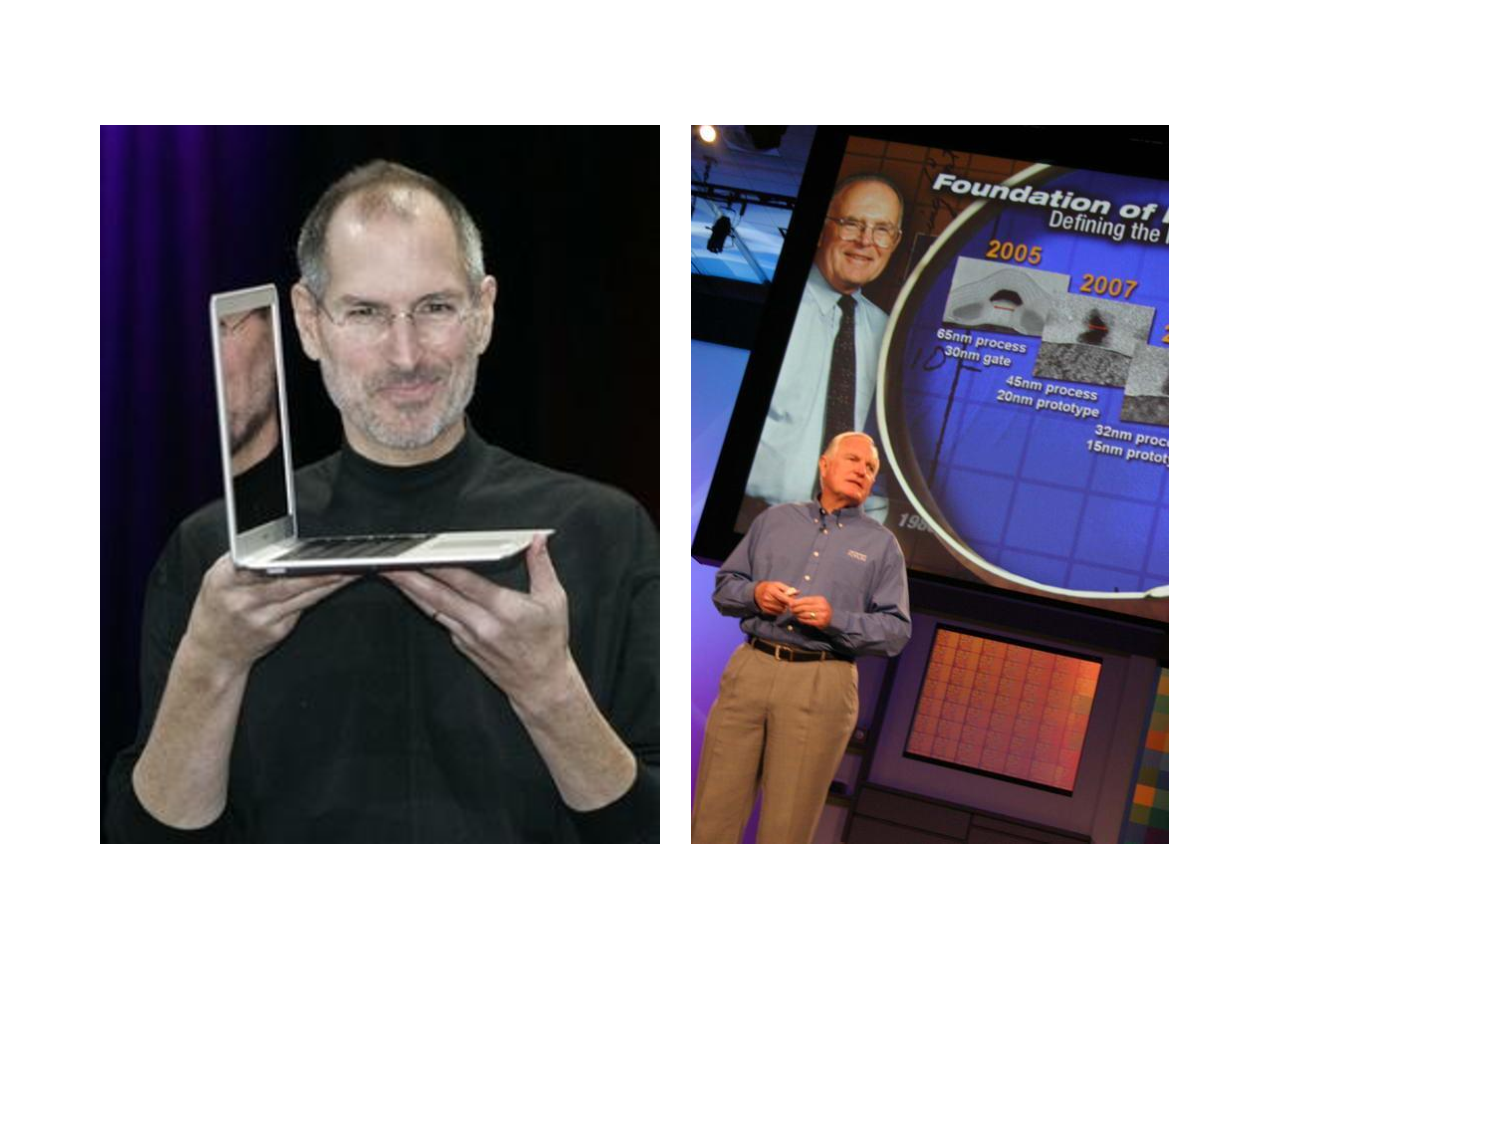
\includegraphics[width= 0.8\columnwidth]{figures/jobs.pdf}
              \caption{(左)乔布斯以及薄如蝉翼的Macbook Air;(右)摩尔定律的提出者戈登·摩尔在演讲
              }
              \label{jobs}
            \end{center}
        \end{figure}

    量子效应和热耗散是经典计算机继续发展下去不可回避的问题。其实,还有一个问题是:经典计算机的
    计算能力极限是多少?一个简单的例子就能说明问题。3乘5等于15,这是一个六七岁的孩子都能回答上的问题。但反过来,15等于
    几乘几呢?虽然这依然是个简单的问题,但它却蕴含了一个可怕的事实:原则上来说经典计算机对这个问题是无能为力的!用科学点的话
    来讲,如果要用经典计算机处理质因数分解的问题,它所需求的时间是指数增长的,在数学上这种问题属于不可求解问题。我们不妨利用一下
    所谓的质因数分解问题来考验一下经典计算机。

    20世纪50年代,真空管计算机大概能够进行每秒1000次的浮点运算,而到了2005年,超级计算机已经可以每秒执行百万亿次的浮点运算,这是一个非常惊人的数字。
    那么,如果我们要分解一个512位的整数需要多久呢?这看上去对我们信赖的计算机应该不是什么难事,但答案却是令人诧异的。如果我们选择每秒能够处理百万次运算的
    芯片,那么这个时间将是8400年!即使使用最强劲的超级计算机,时间花费依然要一个小时之久。如果我们要分解的整数位数增加,计算机分解它所耗费的时间
    更是指数增加的。所以,质因数分解算法是当前最主流的加密算法RSA公钥所采用的加密形式,理论上来说它是牢不可破的,也广泛被应用于政府、军队、银行等重要部门。



    \section{量子计算的应运而生}

    “\emph{底下的空间还大得很。}”

 \hspace{23em} \emph{--理查德·费曼}

其实用应运而生这个词并不准确。量子计算的概念并不是因为经典计算即将到达瓶颈而提出来的。当1959年量子计算的概念第一次提出时\cite{Feynman},经典计算机也只能算刚刚起步(第一台经典计算机Eniac问世于1946年)。
在这次著名的演讲中,费曼给物理学家和工程师们提出了一个有趣的挑战:在\emph{\textbf{很小}}的尺度上
进行操作和控制。特别地,他让听众思考我们能不能建立一种计算机,它的导线直径只有约10到100个原子,而电路仅仅有几百纳米这么大?五十年过去了,现在的半导体工艺已经很接近这个尺度,但费曼的本义并不仅仅是指小,
而是非常非常的小,小到人们要开始考虑量子力学法则:

\emph{“当我们涉及非常,非常小的世界时,比如说7个原子的电路,就会有些有趣的事情出现,可能给予我们新的设计思路。小尺度上的原子行为和大尺度上一点都不同,因为它们仅仅满足量子力学法则。
所以,当我们涉足这个世界的时候,我们必须改变我们的看法,因为我们在和不同的法则一起工作,而这很可能导致我们可以做很多不同的事情。当然,不仅是电路,我们也可以采用一些其他的系统,比如分离的能级,自旋间的相互作用等等。”}

这应该是最早具有量子计算雏形的思想,它充分结合了当时最热门的学科-量子力学的各种推论,描绘了一幅非常诱人的图景。而费曼更是同时给了一个著名的论断:

\emph{“我并不是想违背什么法则。这只是原则上我们可以做到的事情,我们现在还没做到是因为我们实在太大了。”}

经典计算机碰到的下一个问题就是热耗散。既然Landauer认为热耗散来自于逻辑门的不可逆性,那只要说明量子计算是可逆的就可以完全避免这个问题了。Lecerf \cite{Lecerf} 和 Bennett \cite{Bennett}证明,确实可以找到普适的可逆计算,不需要擦除信息,从而也不会产生热耗散。后来, Benioff \cite{Benioff} 发现量子力学的哈密顿量可以被用作普适的经典图灵机模型。换句话说,基于量子力学哈密顿量演化的量子计算是无热耗散的。

真正提出量子计算优越性的还是费曼 \cite{Feynman2,Feynman3}。他认为量子计算机依靠有效模拟其他量子系统的演化,可以做到很多经典图灵机做不到的事情。接着Deutsch发展完善了所谓的量子图灵机模型,并指出量子计算机具有
通过量子并行性来加速计算的潜力 \cite{Deutsch}。

十年之后,量子计算领域第一个真正通过量子并行性取得指数加速的算法,也是让全世界感到震惊的算法-Shor算法 \cite{Shor} 横空出世。之所以说让全世界感到震惊,是因为如上一小节所说,
大多数的部门机构都是采用RSA密钥系统加密,而RSA密钥系统的依据就是大数不能在经典上被有效分解。相对于每秒百万次运算的经典计算机需要8400年来分解一个512位的整数,Shor算法仅需3.5个小时就能
做到这一点!正是由于量子计算的特殊叠加和相干性质,Shor算法可以在多项式的时间复杂度内解决大数分解问题,这在算法上被称作是有效的。该算法提出后,每个国家都会担心自己的安危,一旦在这场信息战中输掉,可能整个国家最
重要的机密就泄露了。也正是由于Shor算法,很多国家都大大增加了量子计算实验研究的投入,因为它的回报实在太大了。

在开始量子计算的全面介绍之前,我们先通过一个耳熟能详的例子展望下量子计算机将怎样改变人们的生活。在文明出现以前,人类就学会了使用光。从最早的摩擦生火产生的火光,到后来的蜡烛和灯笼,再到电发明后
产生的灯泡,所有这些光都有一个共同的性质:非相干性(incoherence)。20世纪60年代,第一台激光器问世了。可能当时谁都不会想到这个在中国被音译为“镭射”的东西会在接下来的半个世纪内给人类带着这么多变化,甚至于夸张点说,
改变了这个世界。最快的刀,最准的尺,最亮的光,无穷无尽的应用,无穷无尽的奇思妙想。你可以用它来逗一下自己的小猫,也可以看球时带着它干扰一下对方的球员;你可以在枪上安装个瞄准镜做到“十步杀一人,千里不留名”,也可以
模仿一下阿纳金,玩一把《星球大战》的cosplay秀。这些都是科学外的应用,而这一切的应用都源于激光的一个性质-相干性(coherence)。

        \begin{figure}[htbp]
            \begin{center}
              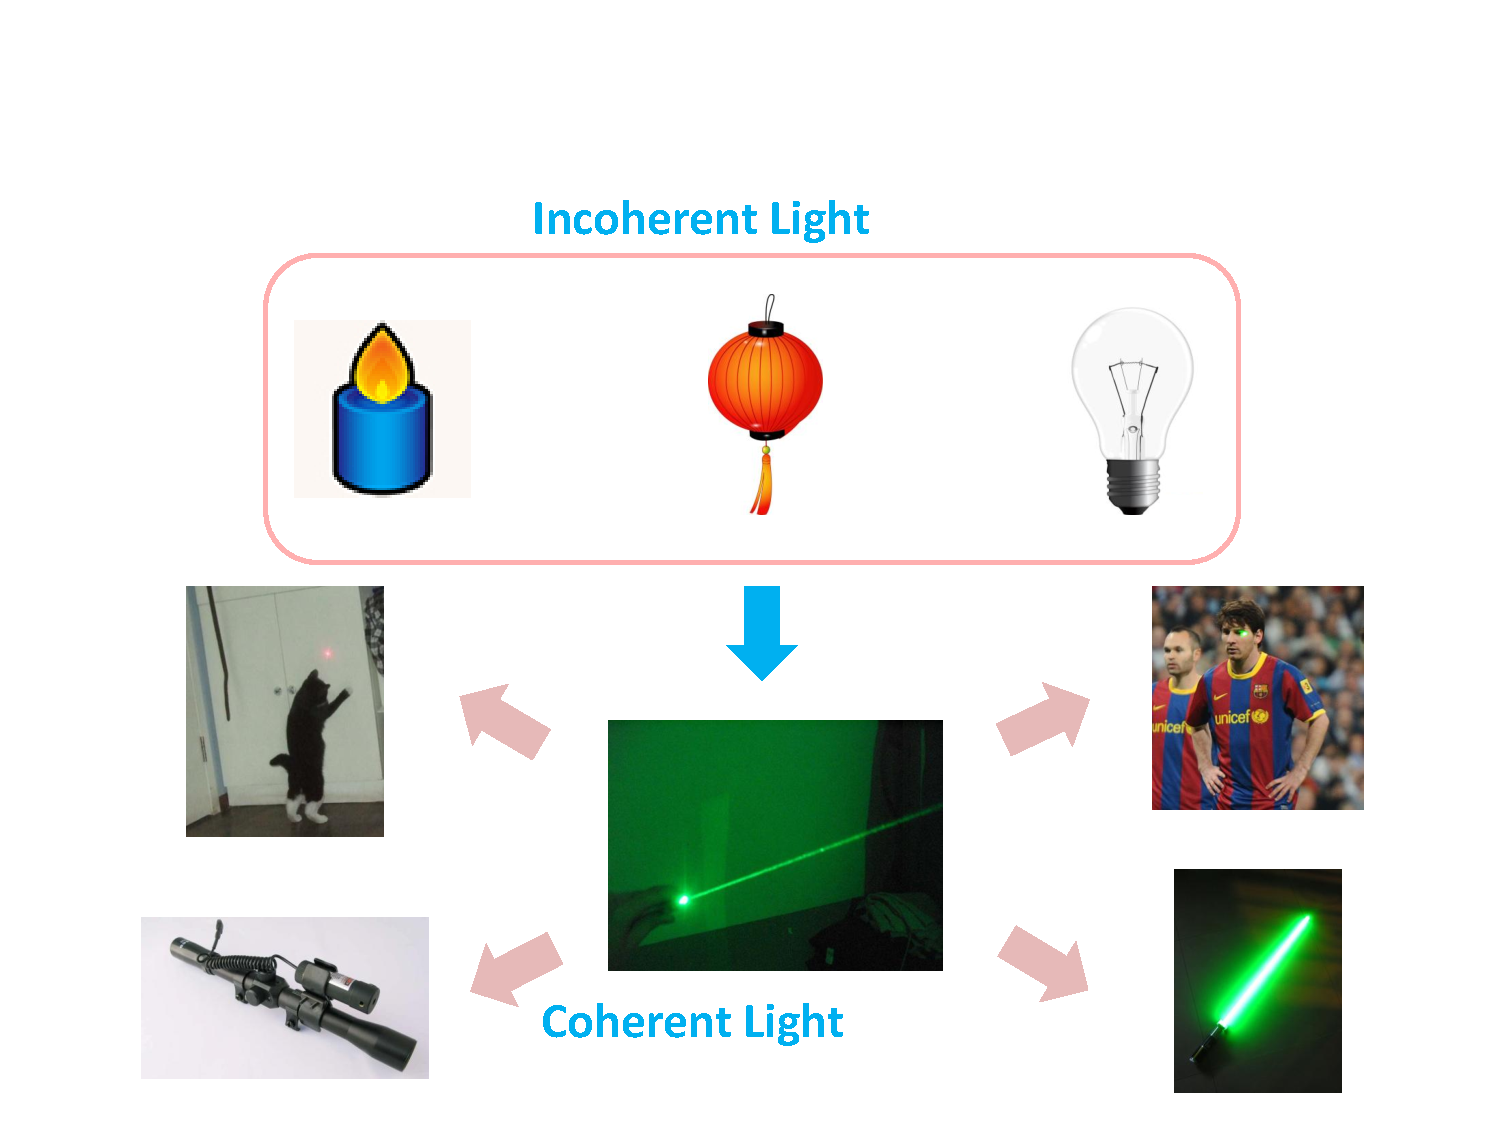
\includegraphics[width= 0.8\columnwidth]{figures/laser.pdf}
              \caption{从非相干光到相干光,人类的生活发生了巨大的改变。从非相干的经典图灵机到相干的量子计算机,人类又将迎来怎样的变化呢?
              }
              \label{laser}
            \end{center}
        \end{figure}

        就如同激光并不是一种新型的经典光,量子计算机也不是新型的经典计算机。它并不能说是快的,或者小的进化型经典计算机,它的进化决不是从电脑到笔记本电脑再到平板电脑的进化这么简单,它将会是一种具有
        全新模式的计算机。指导它工作的不再是长串的01编码,而是量子力学演化。我们想象不到有了量子计算机后生活将发生怎样翻天覆地的变化,目前我们最主要的任务只是
        让这个变化尽早发生。

    \section{量子计算机的工作原理}

    “\emph{当你改变你观看世界的方法的时候,你看到的世界也在改变。}”

 \hspace{23em} \emph{--马克·普朗克}

    在本节中,我们将讨论量子计算的线路模型。事实上,也有更抽象的图灵机模型,两者在物理上是等价的。

    \subsection{量子比特}

    在经典图灵机模型中,储存经典信息的基本单位叫做比特。它是一个二进制变量,其数值一般记做二进制的0或者1。一个比特要么是0,要么是1,正如向空中抛起一枚硬币,那么它落下后
    要么正面朝上,要么反面朝上。我们用二进制的比特理论上可以储存任何信息,最简单的,储存十进制整数就可以利用二进制和十进制的转换。 3=11, 4=100, 50 =110010等等。当然,非整数也是可以写成二进制的形式,像5.5 = 101.1,也就是说任意实数都可以按精度要求用二进制来表示。而在电子学中,很多器件是非常适合二进制表示的,例如电压的高低和开关,电容器的带电荷与否等等,都可以来作为一个比特的载体。

但在量子世界,一切都发生了改变。一个量子的硬币不仅可以正面或反面朝上,它甚至可以同时正反面都朝上,在你观测它之前。著名的薛定谔的猫就是这个道理,这只猫在开箱子,也就是观测之前,它又是死的又是
活的,处于生和死的\emph{\textbf{叠加态}} (superposition state) 上。正是叠加性这个奇妙的性质引出了量子比特(quantum bit, qubit) 的概念。一个量子比特可以认为是一个在二维希尔伯特空间 (Hilbert space) 中描述的两能级量子体系,它可以在数学上被表示为
\begin{equation}
           \left\vert \psi \right\rangle= \alpha  \left\vert 0 \right\rangle + \beta  \left\vert 1 \right\rangle.
 \end{equation}
其中,振幅$\alpha$和$\beta$是任意复数,且满足归一化条件
\begin{equation}
          |\alpha|^2 + |\beta|^2 =1.
 \end{equation}
$\left\vert \psi \right\rangle$就是一个$\left\vert 0 \right\rangle$ 和$\left\vert 1 \right\rangle$的叠加态。$\left\vert \psi \right\rangle$的定义中含有一个不能被任何测量手段观测到且没有物理意义的整体相位,因此我们可以把$\left\vert \psi \right\rangle$写成
 \begin{equation}
           \left\vert \psi \right\rangle= cos\frac{\theta}{2}  \left\vert 0 \right\rangle + e^{i\phi}sin\frac{\theta}{2}  \left\vert 1 \right\rangle.
 \end{equation}
在几何上,我们可以把这个态表示为一个球面上的点,这个球就叫做Bloch球,见Fig. \ref{bloch}。这种基于量子力学的表示形式很容易让人联想到拥有两个自由度$\theta$和$\phi$的经典模拟变量(analog variable),但一个量子比特和经典模拟变量有本质的不同:一个处于 $\left\vert 0 \right\rangle$和 $\left\vert 1 \right\rangle$的叠加态上
的量子比特,从某种意义上来说,是同时处在$\left\vert 0 \right\rangle$态和$\left\vert 1 \right\rangle$态上的!薛定谔猫的概念就是用一种很通俗的说法描述了
量子比特这种奇妙的叠加性。更进一步讲,在一个$n$-qubit的态上,它的自由度是和$n$成指数增长关系的。很快我们就会看到这一点。

        \begin{figure}[htbp]
            \begin{center}
              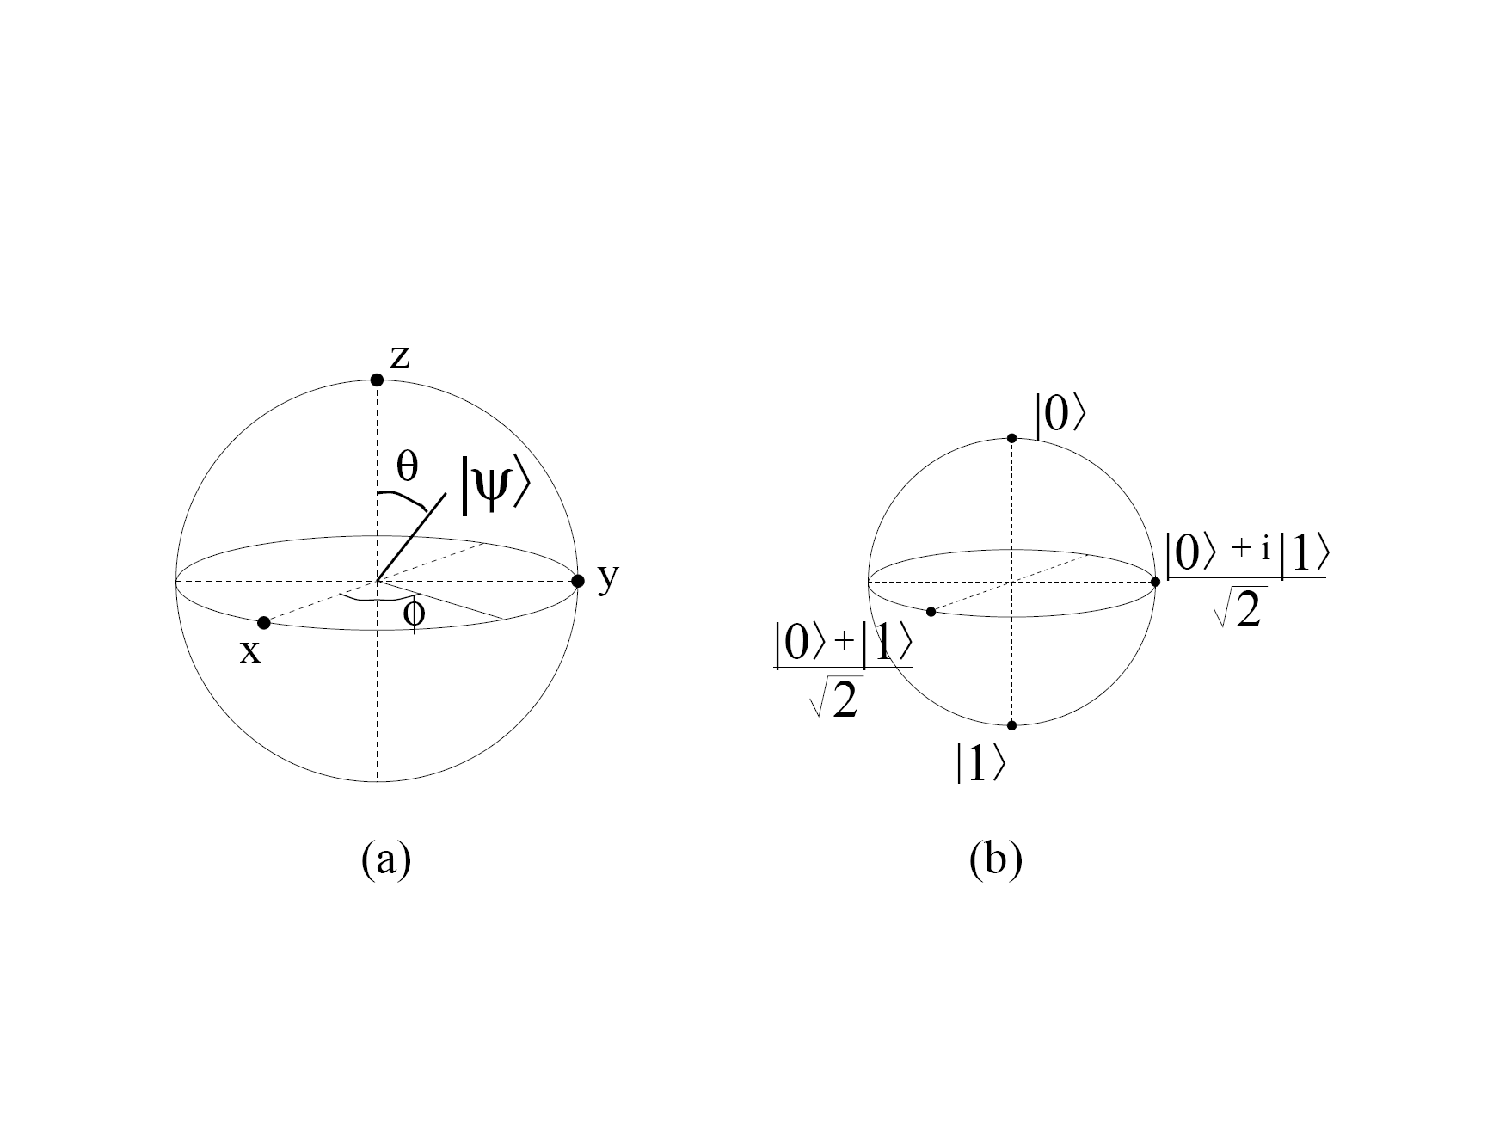
\includegraphics[width= 0.8\columnwidth]{figures/bloch.pdf}
              \caption{(a) 单比特态$ \left\vert \psi \right\rangle$可以用Bloch球上的一个点来表示。(b) Bloch球上的4个重要的点。一般我们把 $\left\vert 0 \right\rangle$态定义为$+\hat{z}$方向。
              }
              \label{bloch}
            \end{center}
        \end{figure}

两个比特的态,假设每一个都处于任意叠加态$ \left\vert \psi \right\rangle_1= \alpha_1  \left\vert 0 \right\rangle + \beta_1  \left\vert 1 \right\rangle$ ,$ \left\vert \psi \right\rangle_2= \alpha_2  \left\vert 0 \right\rangle + \beta_2 \left\vert 1 \right\rangle$ ,则这两个比特的状态可以写成
 \begin{equation}
           \left\vert \psi \right\rangle=\left\vert \psi_1 \right\rangle \otimes \left\vert \psi_2 \right\rangle= (\alpha_1  \left\vert 0 \right\rangle + \beta_1  \left\vert 1 \right\rangle)\otimes( \alpha_2  \left\vert 0 \right\rangle + \beta_2 \left\vert 1 \right\rangle),\label{sepa}
 \end{equation}
 其中$\otimes$是张量积符号,或者叫做直积符号(Kronecker product)。把上式展开,我们能够得到
   \begin{equation}
           \left\vert \psi \right\rangle=  \alpha_1  \alpha_2 \left\vert 0 \right\rangle \otimes \left\vert 0 \right\rangle+\alpha_1  \beta_2 \left\vert 0 \right\rangle \otimes \left\vert 1 \right\rangle+\beta_1  \alpha_2 \left\vert 1 \right\rangle \otimes \left\vert 0 \right\rangle+\beta_1  \beta_2 \left\vert 1 \right\rangle \otimes \left\vert 0 \right\rangle.
 \end{equation}
为了方便,后面我们将省略直积符号$\otimes$, 并把$\left\vert 0 \right\rangle \otimes \left\vert 0 \right\rangle$ 简记为$\left\vert 00 \right\rangle$,以此类推。因此,
 \begin{equation}
           \left\vert \psi \right\rangle=  \alpha_1  \alpha_2 \left\vert 00 \right\rangle +\alpha_1  \beta_2 \left\vert 01 \right\rangle +\beta_1  \alpha_2 \left\vert 10 \right\rangle+\beta_1  \beta_2 \left\vert 11 \right\rangle.
 \end{equation}
 那么,对一个$n$-qubit的寄存器,它的状态可以写成$2^n$个态的叠加,
  \begin{equation}
           \left\vert \psi \right\rangle=  \sum _{i=0}^{2^n-1}c_i \left\vert k \right\rangle.
 \end{equation}
  对这个态的唯一约束条件是归一化条件:
   \begin{equation}
             \sum _{i=0}^{2^n-1} |c_i|^2 =1.
 \end{equation}
 和单比特情形类似,整体相位是可以忽略的。因此,要描述一个$n$-qubit 的纯态需要$2^n-1$个复变量 (混态情形是$4^n-1$个自由度,此处不作详细讨论)。

 在物理实现上,原则上具有叠加性质的两态量子系统都适用做qubit。目前的实验室里,像NMR中
 处于磁场中的自旋1/2粒子(自旋向上和向下),空腔中的原子的态(原子的基态和激发态),超导结之间隧穿的库珀对(Cooper pairs处于一个结和另外一个结时),都可以被用作qubit。当然,如果一个硬币可以同时向上和向下也是可以的,在量子随机行走
 中我们就会看到这种量子硬币(quantum coin)。

 现在我们可以回过头来在看一下经典计算机和量子计算机的差距,这次是存储容量上的。
 考虑一个简单的情况,我们要储存45个自旋1/2的粒子,这在量子系统中只是一个很小的体系,只需要45个qubit就可以实现。但如果我们要用经典
 计算机完成这个任务,约需要$2^{45}$个经典比特,也就是大概4个TB的硬盘!这里有些典型的数据来跟它比较,4TB大概是4,000G或者4,000,000M,而一部高清蓝光电影大概是10G,一本书大概是5M,编写本论文的Tex软件包
也只有2G。另外一些比较有意思的数据是,美国国会图书馆的所有藏书总容量大概为160TB或者说50个qubit,而2007年人类所拥有的信息量总和为$2.2\times 10^9$个TB
\cite{Hilbert},也仅相当于71个qubit的存储容量。
 \begin{figure}[htbp]
            \begin{center}
              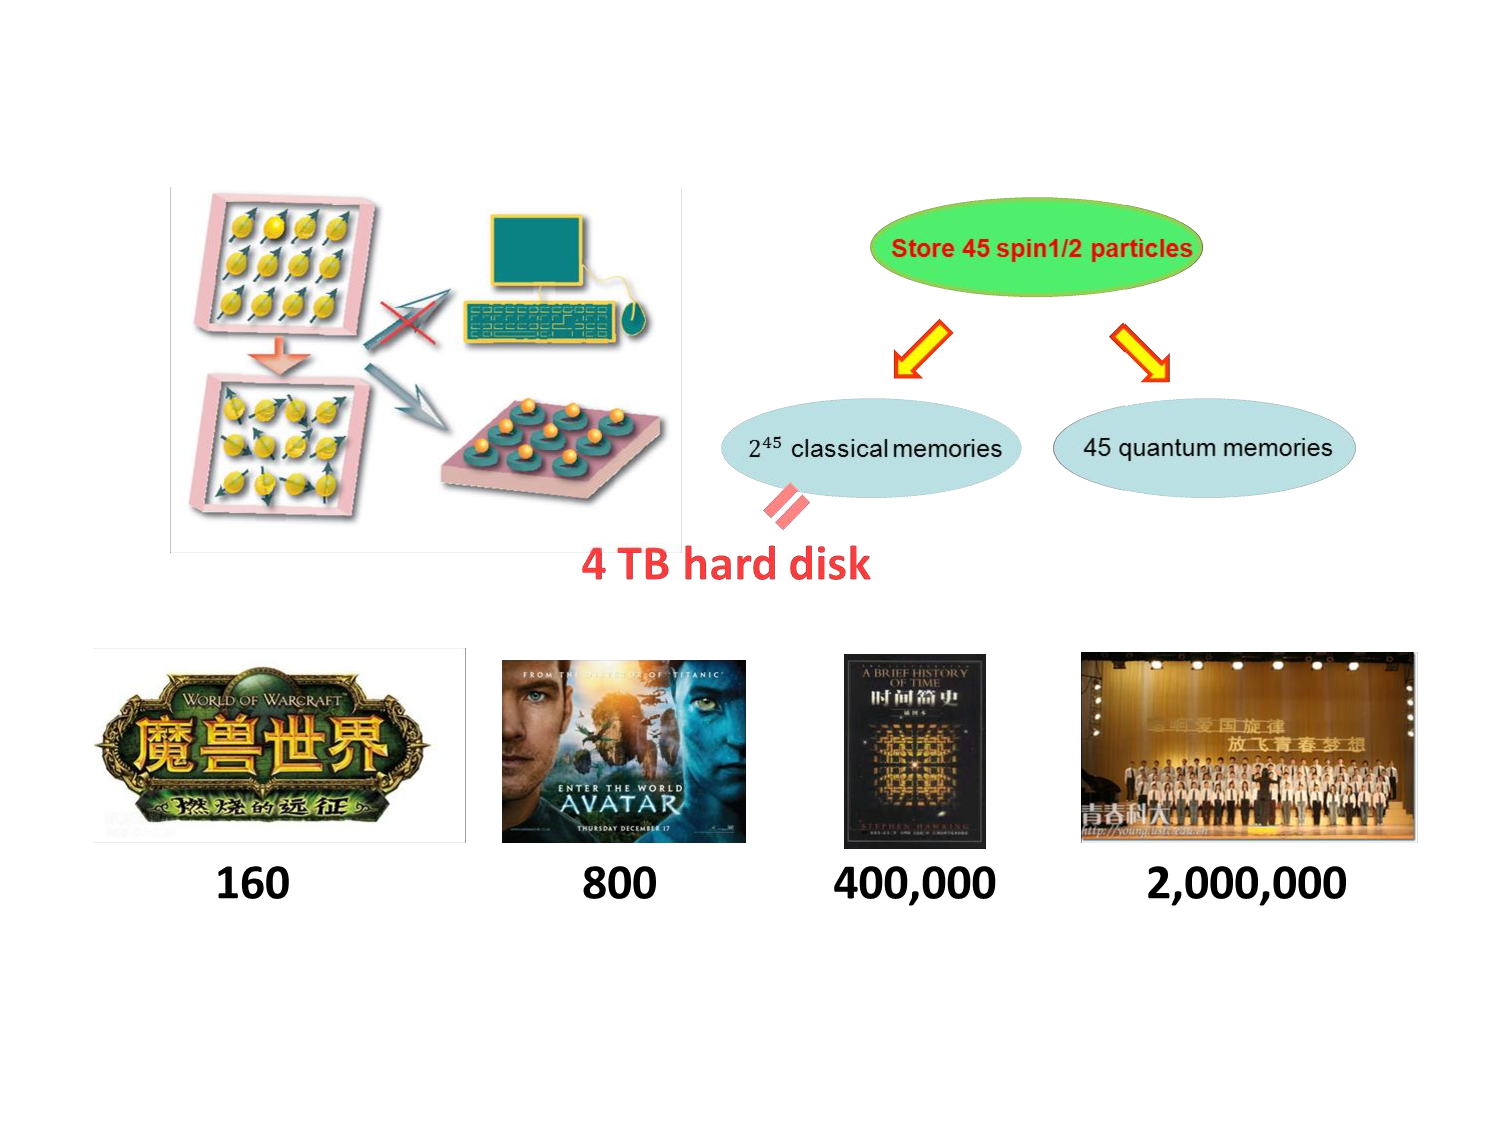
\includegraphics[width= 0.8\columnwidth]{figures/register.pdf}
              \caption{要储存45个自旋1/2的粒子,我们需要45个量子比特或者$2^{45}$个
              经典比特。用这些经典比特组成的硬盘我们可以做很多事情,比如存放160个《魔兽世界》,800部
              《阿凡达》,40万本《时间简史》或者200万首《永恒的东风》。仅仅从存储量上看,经典计算机已经输了。
              }
              \label{register}
            \end{center}
  \end{figure}

\subsection{量子纠缠}

虽然叠加原理赋予了量子计算机 可以在一次运行中完成指数次运算的机会, 也就是并行性计算模式,但叠加性并不是量子系统独有的。事实上,也存在满足叠加性原理的经典波,比如两端固定的弦震动方程。但和量子系统不同的是,这些所谓的叠加
能级必须属于同一个系统,属于不同系统的经典态是永远不能叠加起来的,也就是没有\textbf{纠缠}(entanglement)的。如果一个多比特量子态能够被
写成各个比特的态的直积形式,那么我们就说这个态是可分离(separable)的,比如Eq. \ref{sepa} 。

相反地,我们总可以找到合适的$\alpha_1, \beta_1$和$\alpha_2, \beta_2$,使得$ \left\vert \psi \right\rangle_1= \alpha_1  \left\vert 0 \right\rangle + \beta_1  \left\vert 1 \right\rangle$ 和$ \left\vert \psi \right\rangle_2= \alpha_2  \left\vert 0 \right\rangle + \beta_2 \left\vert 1 \right\rangle$ 直积之后的结果为
 \begin{equation}
         \frac{\left\vert 00 \right\rangle+ \left\vert 11 \right\rangle}{\sqrt{2}},
 \end{equation}
 那么不论我们如何分解,它都是不可能被写成两个qubit的态的直积形式的。这种情况我们就称这个态是不可分离(non-separable)的或者\textbf{纠缠}(entangled)的。后面我们会看到,
 纠缠是量子计算中最重要的资源之一,绝大部分的量子算法加速都源于量子纠缠。当然,近些年有理论研究表明纠缠并不是量子算法加速必不可少的资源,还存在着一种
 叫做量子无序(quantum discord)的资源比纠缠的实用范围更加广泛,具体这部分研究可以参考其他文献。

 \subsection{量子态的演化和量子逻辑门}

 前面我们给出了量子比特的\textbf{静态}性质,讲了量子寄存器的存储方法以及重要的量子纠缠资源。这一小节我们将着重于研究怎么用一种可控的方式来实现我们的
 计算任务,也就是量子比特的\textbf{动态}性质。

 在一个封闭的量子系统中,态的演化是满足薛定谔方程的
  \begin{equation}
         i\hbar \frac{d\left\vert \psi(t)\right\rangle}{dt}=H\left\vert \psi(t)\right\rangle,
 \end{equation}
其中 $\hbar$是普朗克常数,$H$是整个系统的哈密顿量。对于不含时(time-independent)的哈密顿量来说,
薛定谔方程有很简单的解
   \begin{equation}
       \left\vert \psi(t)\right\rangle = e^{-iHt/\hbar} \left\vert \psi_0\right\rangle,
 \end{equation}
 $\psi_0$是$t=0$时系统所处的态。一般,我们用幺正算子$U$来定义时间演化算子,即
    \begin{equation}
       U = e^{-iHt/\hbar},
 \end{equation}
 也就是说,
   \begin{equation}
       \left\vert \psi(t)\right\rangle =U \left\vert \psi_0\right\rangle.
 \end{equation}
 如果用密度矩阵的语言,那么量子系统的密度矩阵演化可以写成
    \begin{equation}
       \rho(t) = \left\vert \psi(t)\right\rangle \left\langle \psi(t)\right\vert = U\rho_0 U^{\dagger}.
 \end{equation}
 在后面的章节中,为了方便我们将把普朗克常数$\hbar$的值设为1。

 一般来说,在简单的量子系统中,一般包含单粒子项和两粒子间的相互作用项。三体及以上的相互作用
 至今还没在实验中被观测到。因此,我们能够实现的量子逻辑门都是单比特门或两比特门。很幸运的是,
 后面我们将看到,任何幺正操作$U$都是可以拆解成单量子门和\textbf{受控}两比特门的组合的 \cite{Deutsch2,DiVincenzo2,Lloyd2,DBE}。 我们将在下面分别讨论单量子们和两比特门。

 最简单的单比特门是非门(NOT gate)。和经典情况类似,非门的作用是可以把 $\left\vert 0\right\rangle$ 和 $\left\vert 1\right\rangle$ 相互翻转。非门的矩阵形式是
     \begin{equation}
       U_{NOT} = \left(
                   \begin{array}{cc}
                     0 & 1 \\
                     1 & 0 \\
                   \end{array}
                 \right).
 \end{equation}
 如果输入态是任意态
  \begin{equation}
       \left\vert \psi\right\rangle =\left(
                                                                       \begin{array}{c}
                                                                         \alpha \\
                                                                         \beta \\
                                                                       \end{array}
                                                                     \right),
 \end{equation}
 那么非门作用后
      \begin{equation}
       U_{NOT}\left\vert \psi\right\rangle = \left(
                   \begin{array}{cc}
                     0 & 1 \\
                     1 & 0 \\
                   \end{array}
                 \right)\left(
                                                                       \begin{array}{c}
                                                                         \alpha \\
                                                                         \beta \\
                                                                       \end{array}
                                                                     \right) = \left(
                                                                       \begin{array}{c}
                                                                         \beta \\
                                                                         \alpha \\
                                                                       \end{array}
                                                                     \right).
 \end{equation}
 另外一种重要的单比特量子门叫做Hadamard门,其定义为
      \begin{equation}
       H =\frac{1}{\sqrt{2}} \left(
                   \begin{array}{cc}
                     1 & 1 \\
                     1 & -1 \\
                   \end{array}
                 \right).
 \end{equation}
 经过Hadamard门后,$\left\vert 0\right\rangle$ 和 $\left\vert 1\right\rangle$将分别变成 $\left\vert +\right\rangle$ 和 $\left\vert -\right\rangle$ ,即
   \begin{eqnarray}
       &&H\left\vert 0\right\rangle =\frac{1}{\sqrt{2}} (\left\vert 0\right\rangle+\left\vert 1\right\rangle)\equiv \left\vert +\right\rangle,\nonumber \\
        &&H\left\vert 1\right\rangle =\frac{1}{\sqrt{2}} (\left\vert 0\right\rangle-\left\vert 1\right\rangle)\equiv \left\vert -\right\rangle.
 \end{eqnarray}

 实际上。任意的单比特操作都可以写成如下形式
 \begin{equation}
      U = e^{i\alpha}R_{\hat{n}}(\theta),
 \end{equation}
 其中$R_{\hat{n}}(\theta)$对应于Bloch球上的旋转操作,绕$\hat{n}=(n_x,n_y,n_z)$轴旋转$\theta$角。
 在定义了泡利矩阵(Pauli matrices)后
 \begin{equation}
      \sigma_x\equiv \left(
                       \begin{array}{cc}
                         0 & 1 \\
                         1 & 0 \\
                       \end{array}
                     \right),  \sigma_y\equiv \left(
                       \begin{array}{cc}
                         0 & -i \\
                         i & 0 \\
                       \end{array}
                     \right),  \sigma_z\equiv \left(
                       \begin{array}{cc}
                         1 & 0 \\
                         0 & -1 \\
                       \end{array}
                     \right),
\end{equation}
我们就可以把单比特旋转操作用泡利算子展开
\begin{equation}
    R_{\hat{n}}(\theta)\equiv e^{-i\frac{\theta\hat{n}\cdot\overrightarrow{\sigma}}{2}}  = cos(\theta/2)\sigma_I - isin(\theta/2)[n_x \sigma_x+n_y \sigma_y+n_z \sigma_z].
\end{equation}

两比特门中最常见的是控制非门(controlled-NOT gate, CNOT gate)。在CNOT门中第一个比特起控制作用,第二个比特为目标比特。当控制比特处于 $\left\vert 0\right\rangle$时,受控非门不进行操作。当控制比特处于 $\left\vert 1\right\rangle$时,目标比特进行翻转操作。CNOT门的作用可以表示成
 \begin{equation}
    U_{CNOT} \left\vert \psi_1\right\rangle \left\vert \psi_2\right\rangle = \left\vert \psi_1\right\rangle \left\vert \psi_1\oplus \psi_2\right\rangle (\psi_1,\psi_2 = 0,1),
\end{equation}
$\oplus$是模2操作。写成矩阵形式的话,CNOT门是$4\times4$的
 \begin{equation}
    U_{CNOT} = \left(
                 \begin{array}{cccc}
                   1 & 0 & 0 & 0 \\
                   0 & 1 & 0 & 0 \\
                   0 & 0 & 0 & 1 \\
                   0 & 0 & 1 & 0 \\
                 \end{array}
               \right).
\end{equation}
该形式为比特1控制比特2的CNOT门形式。还有一种重要的两比特门叫做SWAP门,它的作用
是把两个比特的状态进行交换,值得注意的是SWAP门不是受控的。它的矩阵形式是
 \begin{equation}
    U_{SWAP} = \left(
                 \begin{array}{cccc}
                   1 & 0 & 0 & 0 \\
                   0 & 0 & 1 & 0 \\
                   0 & 1 & 0 & 0 \\
                   0 & 0 & 0 & 1 \\
                 \end{array}
               \right).
\end{equation}

主要的两比特门在量子线路图中用如下符号表示:
\begin{figure}[htbp]
            \begin{center}
              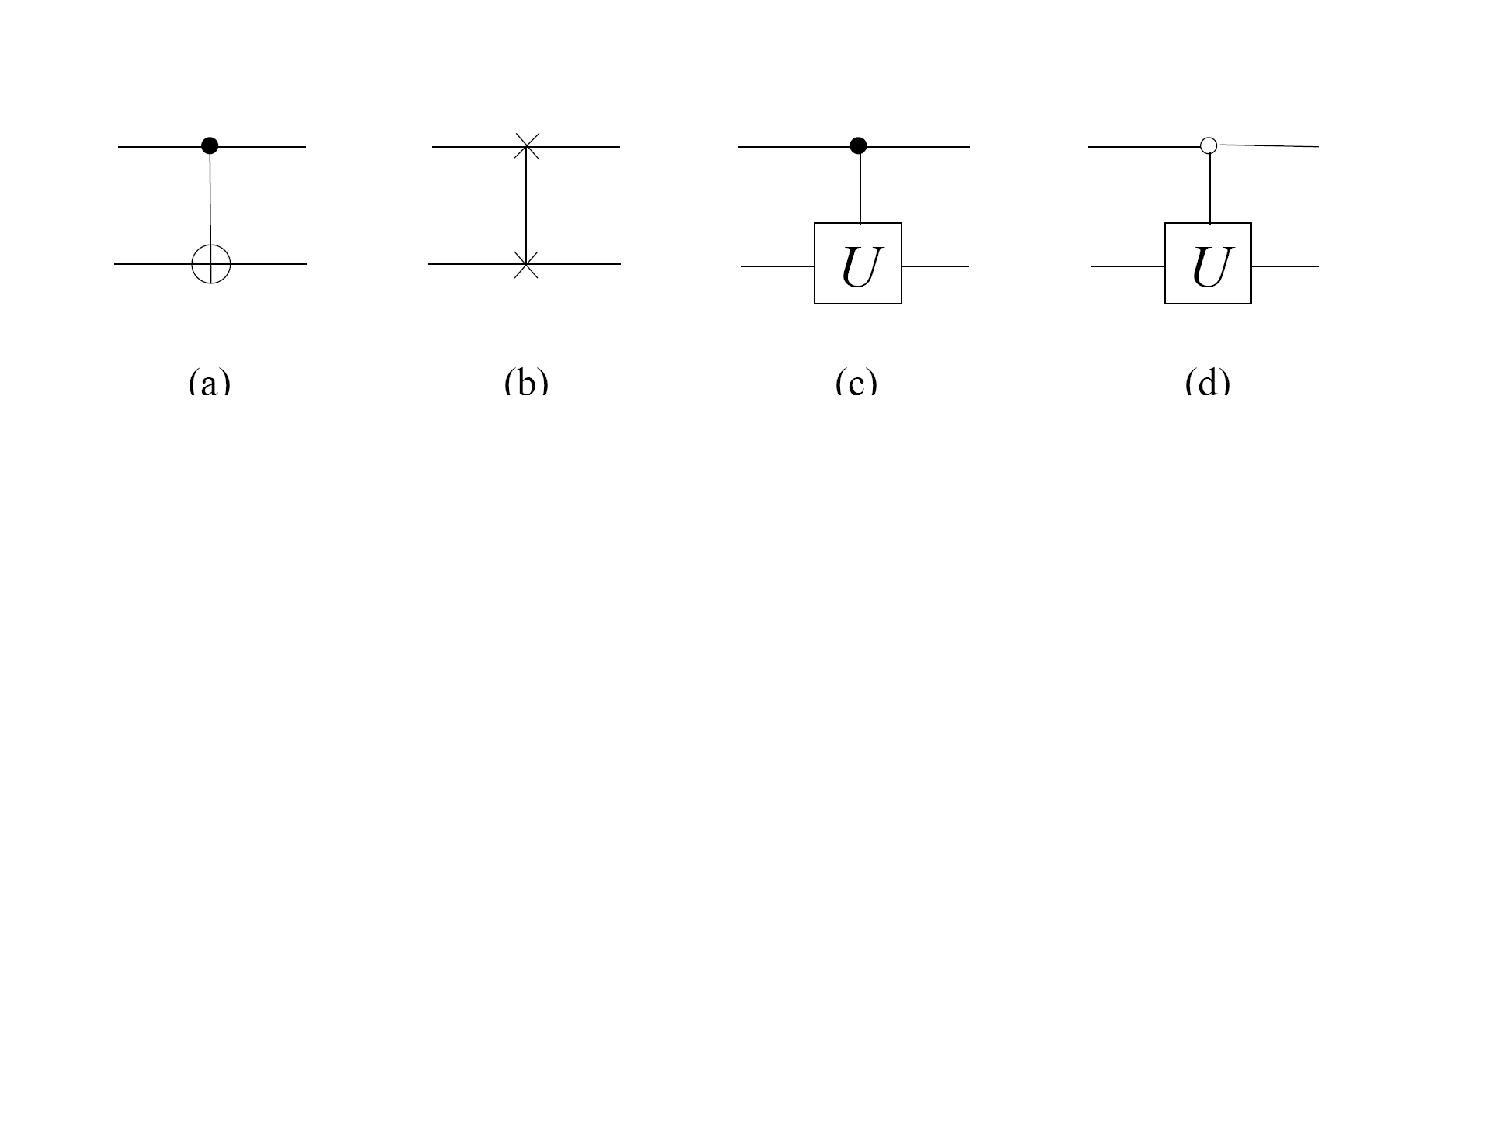
\includegraphics[width= 0.8\columnwidth]{figures/cnot.pdf}
              \caption{几种常用的两比特量子门(a) CNOT$_{12}$门,(b) SWAP门,(c) 控制U门,(d) 0控制U门。
              }
              \label{cnot}
            \end{center}
  \end{figure}

事实上,对于多比特系统,更重要的是如下关于量子线路分解的定理:

\emph{任意的量子门都可以分解为CNOT门和单比特旋转门的组合。}

有了以上定理,如果我们能找到有效的分解算法,那么原则上我们可以实现
任意复杂的量子线路图。

\subsection{量子态的测量}

在量子力学的假设中,对一个量子系统的任意测量操作总可以用一组测量算子
$P_m$来描述。对一个处于$\left\vert \psi\right\rangle$态的量子系统,经过观测算子 $P_m$后得到结果为$m$的概率为
\begin{equation}
    p(m) =\left\langle \psi \right\vert P_m \left\vert \psi\right\rangle.
\end{equation}
测量后,该量子系统将塌缩为
\begin{equation}
    \frac{P_m \left\vert \psi\right\rangle}{\left\langle \psi \right\vert P_m \left\vert \psi\right\rangle}.
\end{equation}
这组测量算子的集合必须满足完备性关系
\begin{equation}
  \Sigma_m P_m = I,
\end{equation}
才能保证所有概率$p(m)$之和为1。特别的,对于投影测量(projective measurement),我们还要求 $P_m$是厄米算子并且
\begin{equation}
P_m P_{m'} = \delta_{mm'}P_m.
\end{equation}
因此,我们可以利用一组正交基$\left\vert m \right\rangle$来定义任意投影算子的集合,简单的比如$P_m = \left\vert m \right\rangle \left\langle m \right\vert $。在这组投影测量下,得到$m$的概率为
 \begin{equation}
    p(m) = |\left\langle m \right\vert \psi  \rangle |^2,
\end{equation}
且测量后的态为$\left\vert m \right\rangle$。

如果我们在$\{ \left\vert 0 \right\rangle , \left\vert 1 \right\rangle\}$基中测量单比特态$ \alpha  \left\vert 0 \right\rangle + \beta  \left\vert 1 \right\rangle$ ,那么我们得到$\left\vert 0 \right\rangle$ 的概率为$|\alpha|^2$,得到$\left\vert 1 \right\rangle$ 的概率为$|\beta|^2$。

当然Stern-Gerlach实验早就证明对于量子系统被测量后的塌缩性质,也就是我们
不可能通过对一个qubit进行连续测量来得到其系数$\alpha$和$\beta$。当然,一个直接的
想法是如果我们可以在大量该粒子的拷贝上进行足够多的投影测量,总能通过统计规律
得到$\alpha$和$\beta$的值。但很遗憾,不可克隆定理(no-cloning theorem)\cite{Dieks,nocloning}告诉我们这也是不行的,因为我们不能对一个处于未知态的
qubit进行精确的拷贝(或许可以预见盗版量子计算机的软件将是一个技术活)。 总结来说,

\emph{没有测量手段可以完全揭示一个处于未知态的量子比特的状态。}

关于量子计算的基本原理的参考书目及文献很多。值得推荐的有:

Nielsen和Chuang的名作《量子计算与量子信息》\cite{yellow},国内被昵称为“黄书”(因其中文版封面为黄色);
非常基础的Steane写的review \cite{steane},当然这篇文献的部分内容已经非常过时;
Preskill的讲稿 \cite{Preskill};Bennett和DiVincenzo写的权威性评述 \cite{benben};Benenti, Casati和Strini合著的《量子计算与量子信息原理》\cite{wangwenge}(中文版为王文阁,李保文等译)。

\section{量子计算机的物理实现}

    “\emph{我们要记住,或许有一天量子理论会被证明是失败的,因为它和我们日常的生活经验、哲学是如此的不同。}”

 \hspace{23em} \emph{--理查德·费曼}

上一节的内容已经从理论上大致描绘了一台量子计算机的蓝图,但在真正的量子计算机问世之前,一切都是空话。
理论上已经提出了很多方案可以物理实现量子计算,但对大规模量子系统的精确控制存在着很多困难,比如退相干效应。在宏观
世界中,我们很难观测到量子行为的一个重要原因就是退相干已经把量子性彻底给退光了。但是,随着技术的日新月异以及更有潜力的量子计算方案的提出,
人们距离真正的量子计算机还是越来越近的。2011年,加拿大的D-Wave公司就宣称他们已经成功研制了世界上第一台通用量子计算机 \cite{dwave},包含128个qubit,售价为1000
万美金。美国的Lockheed Martin公司斥巨资购买了一台,但业内人士对这个号称基于绝热量子计算的庞然大物 普遍存在质疑,认为它并不能做到真正的单qubit控制,且能解决的任务非常有限。本文不会对这个争议颇多的“量子计算机”作更多的讨论,更重要的是分析当前各量子计算方案的利弊,
力图给出各方案的发展前景。

 \begin{figure}[htbp]
            \begin{center}
              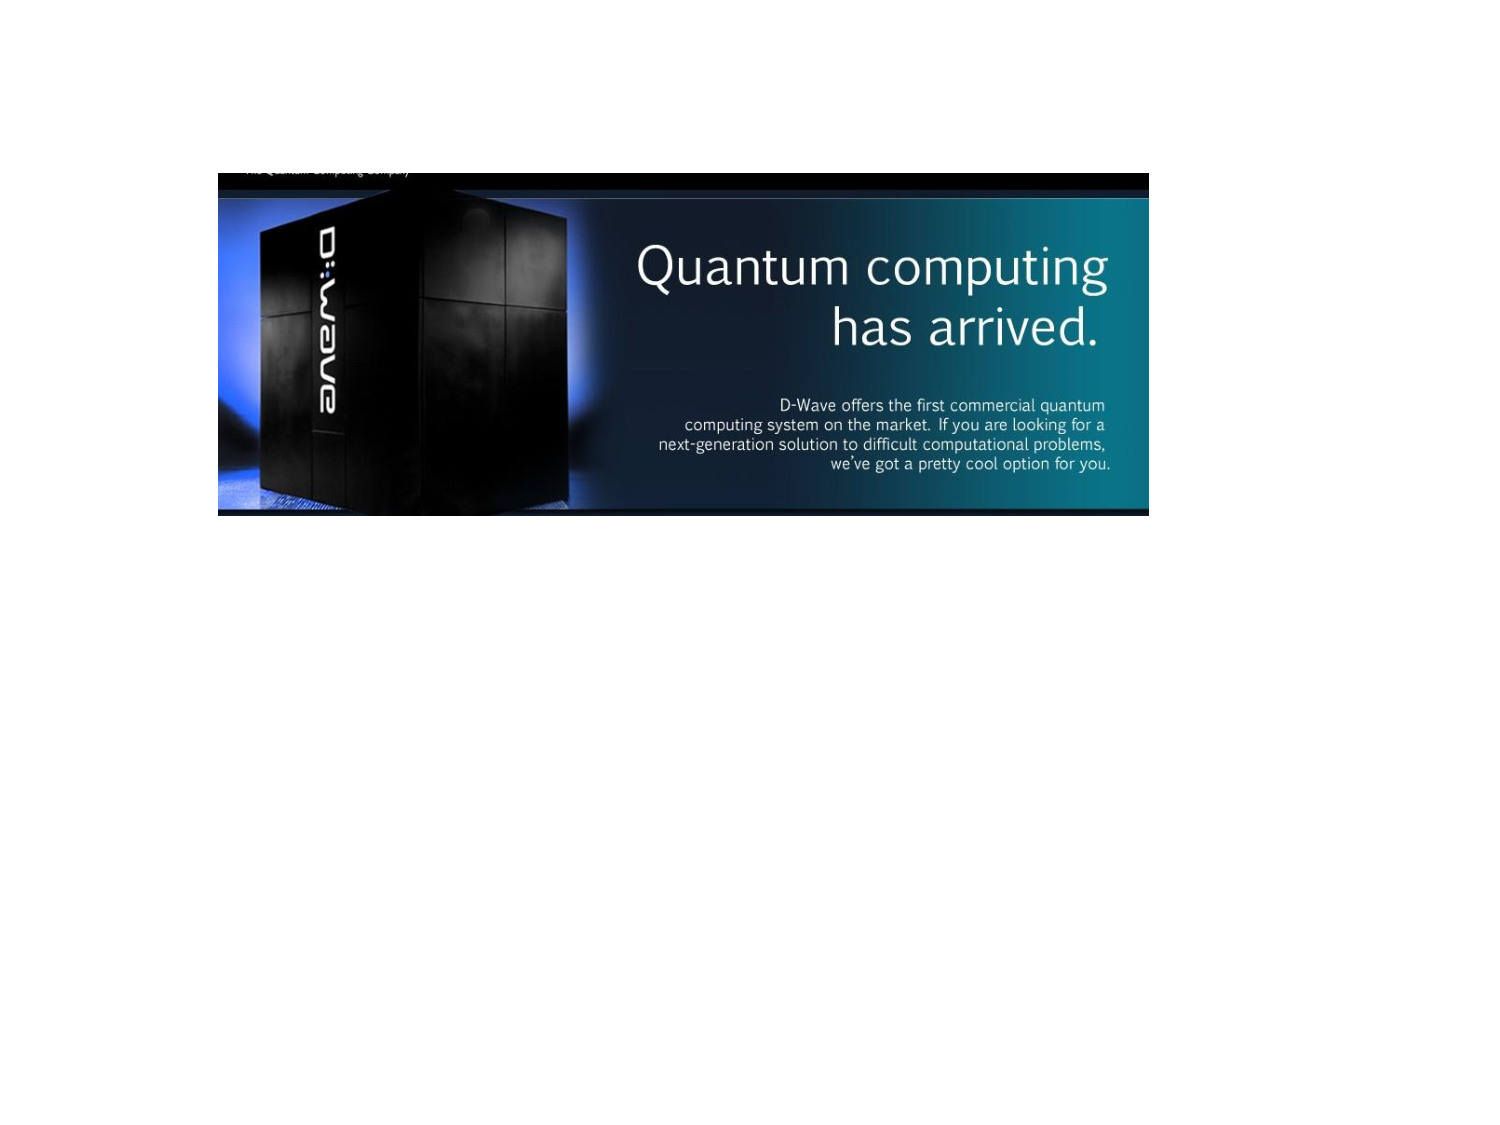
\includegraphics[width= 0.8\columnwidth]{figures/dwaveqc.pdf}
              \caption{加拿大D-Wave公司宣称他们已经制造出第一台128-qubit的超导量子计算机,但谁也不知道这个售价高的吓人(1000万美金)的超大黑盒子里藏的是什么。
              }
              \label{dwave}
            \end{center}
  \end{figure}

  \subsection{量子计算机的要求}

或许对量子计算机最苛刻,也是最普适的要求是所谓的“封闭盒子”(close box)条款:在操作人员的控制下所执行的量子计算机的内部操作,必须和整个宇宙的其他部分孤立开来。即使一点点的干扰都可能让我们脆弱的量子计算机产生毁灭性的
衰亡,也就是\textbf{退相干}(decoherence)。

退相干有多种来源。在大量实验的系综测量中,由于哈密顿量是含时的,导致每次的振荡频率总会有差别,统计下来整个设备就会有信号衰减,这个时间尺度叫做$T_2^{\ast}$;实验中,系统总会被附加一些随机的过程或者放出能量,
导致统计结果为系统朝热平衡态演化,这个时间尺度叫做$T_1$;而系统也可能和外界环境通过相互作用让振荡产生相位扰动,导致相干的衰减,这个时间尺度叫做$T_2$。一般来说,$T_2\leq 2T_1$,而且在绝大多数系统中,$T_1 \gg T_2$,所以在量子计算中$T_2$是更加重要的。

没有什么系统是完全的退相干不变的,但是少量的退相干影响是可以通过各种技术消除的,著名的比如\textbf{量子纠错}(quantum error correction)。早期的对容错量子计算机的物理实现要求有著名的DiVencenzo五条定则\cite{DiVincenzo5},这里不再赘述。如果我们假设物理体系的退相干效应足够小的话, 一个物理实现方案只需要满足下面三个条件就可以用做量子计算机的潜在体系了。

首先是\textbf{可扩展性}(scalablity)。量子计算机的操作都是在Hilbert空间中进行的,而Hilbert的空间维度是指数形式增长的,这就要求我们的物理体系要有非指数的资源,但却
能反应出Hilbert空间的指数增长,例如时间,空间,能量等。标准的做法就是遵循 DiVincenzo的第一条定则:可以简单的对一个系统增加新的且可分辨的qubit。当然要宣称一个方案是“可扩展的”确实非常难,因为用来定义和操控qubit的资源总是多种多样的,这会涉及到很多经典技术,比如
微芯,微波,激光,低温等。为了证明该方案可扩展,必须同时要把这些技术做到可扩展,这可能就需要非常复杂的工科知识了。

其次是该体系有能执行\textbf{普适的逻辑操作}。也就是,在大的Hilbert空间中的操作必须能够分解成一系列简单的操作,而这些简单操作的需求资源不能是指数增长的。当然,前面已经
说过,任意角度的单比特旋转门和两比特CNOT门就可以组合成任意的逻辑操作,也就是说只要该体系能够有效实现这两个门就可以了。当然,出了基于逻辑门的量子计算,还有其他的量子计算模式,比如
绝热量子计算(adiabatic quantum computation)\cite{adia1},单向量子计算(one-way quantum computation)\cite{oneway1}等。这些量子计算模式中和基于逻辑门的量子计算是等价的,但执行它们并不需要拆解逻辑门。

最后是\textbf{纠错能力}(correctability)。该方案必须能够萃取计算机的信息熵来得到有用的量子态,比如有效的初态制备和测量。初态制备其实就是把一个量子系统迅速
地冷却到低熵的状态,而测量就是迅速地以较高的精度得到量子系统的状态的能力,这两者在某种意义上是相似的,且已经被统一到了量子纠错理论中。

目前建造量子计算机最主要的挑战就是操控,测量量子系统的能力,以及阻止系统和外界环境的相互作用的能力,我们将对目前主流的备选方案进行基本介绍。

  \subsection{光学量子计算}

相比于其他系统,光子的退相干效应要小很多,非常适合用作qubit。qubit的信息可以编码到光子的极化状态上,而单比特旋转可以通过线性光学器件,如分束器,相移器等 轻松实现,但如何达到需求的相互作用
从而实现两比特门一直是一个难题,采用非线性Kerr介质中的原子来传递在技术上非常困难。2001年,著名的KLM(Knill-Laflamme-Milburn)方案出现\cite{KLM},表明通过单光子源,单光子探测器以及线性光学线路是可以实现普适量子计算的。
其条件是在量子计算过程中的任意阶段,都可以用单光子探测器进行测量,且测量结果可以用来控制其他光学单元。目前,实验上已经有一些简单的量子算法在线性光学系统上
得到了验证\cite{optics1,optics2}。最近的工作主要集中在如何实现高效率的单光子源\cite{optics5,optics6}和单光子探测器\cite{optics3,optics4}上。

 \begin{figure}[htbp]
            \begin{center}
              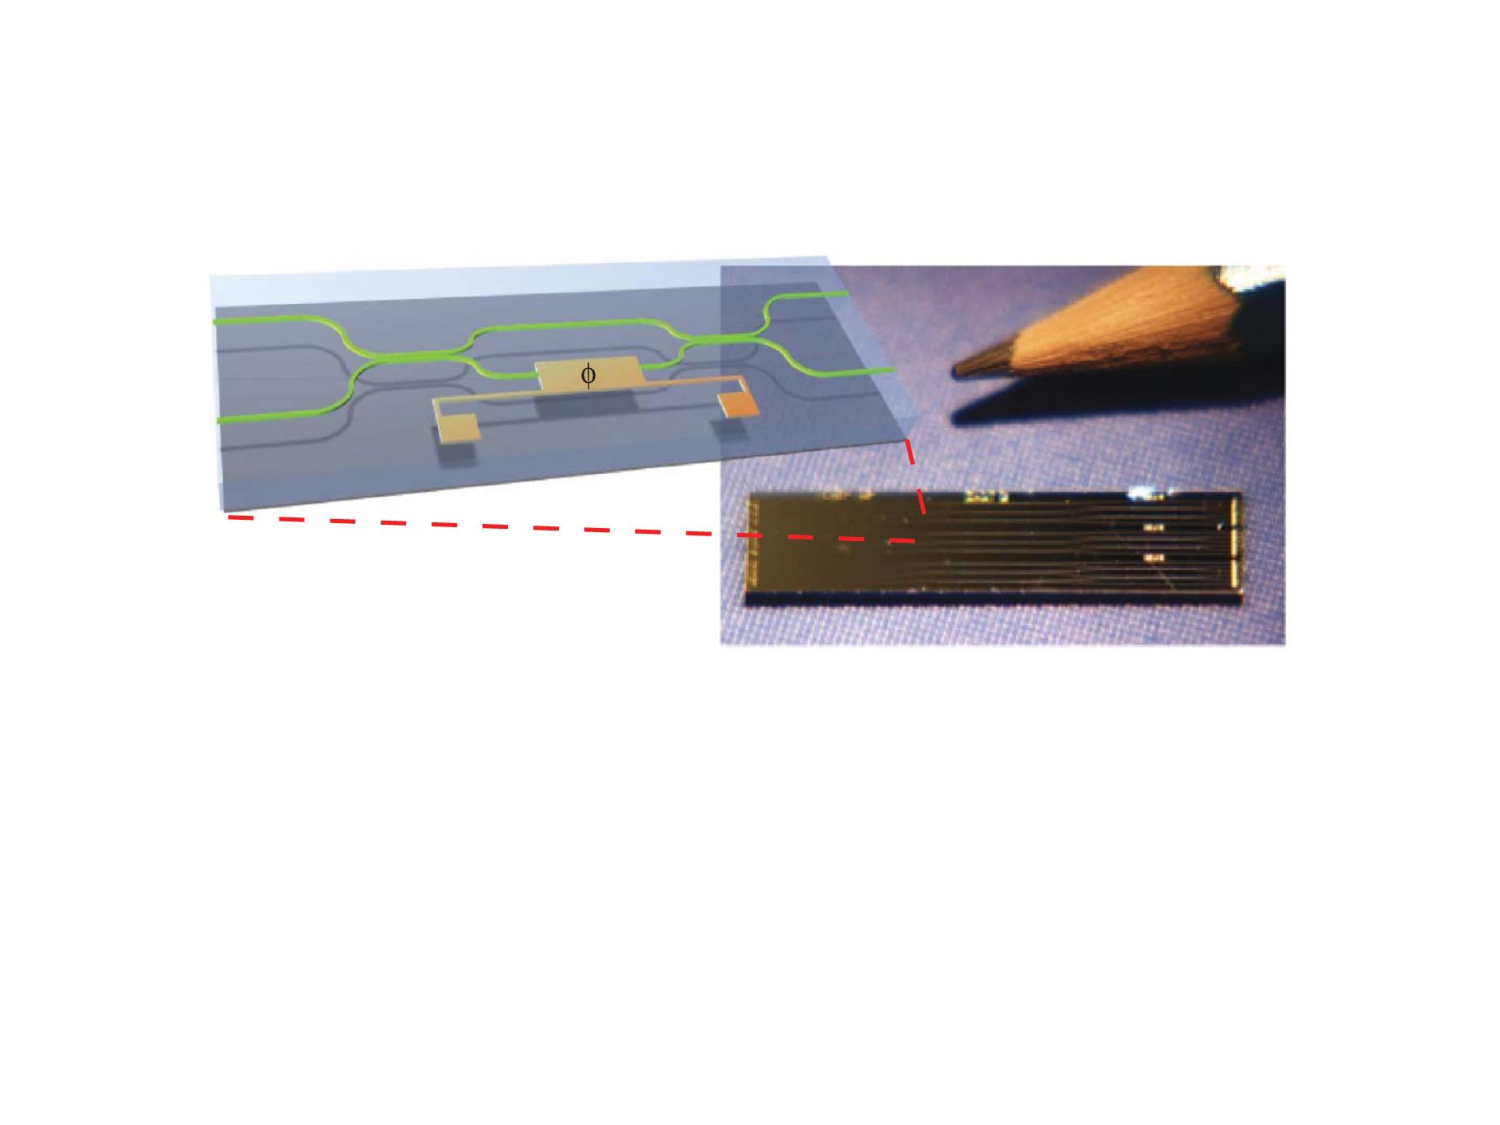
\includegraphics[width= 0.8\columnwidth]{figures/optics.pdf}
              \caption{光学量子计算机的示意图,一个微芯包含几块硅制波导干涉仪以及光控制相移器。绿色的线是光波导,黄色部分是金属制接触器。取自[Nature Photon. 3,
346 (2009)\cite{optics7}]
              }
              \label{photon}
            \end{center}
  \end{figure}

 \subsection{囚禁原子量子计算}

相对于其他体系,在囚禁原子和离子中,由于与环境的相互作用非常弱,所以该体系的退相干时间
非常长,典型的$T_2$已经为几秒,这是该体系作为量子计算方案的最大优势。

 在囚禁原子中,首先出现的是离子阱量子计算。把一个静电场和交变电场联合起来,然后将一串离子束缚于一个线性势阱之中。这些离子构成了qubit,而离子的两个能级则对应于qubit的两个态。单量子比特门
 可以通过对离子施加激光脉冲实现,而qubit之间的相互作用可以通过离子串的集体振动模式来传递,从而形成受控两比特门\cite{ions1,ions2}。2001年,Cirac和Zoller\cite{ions3}构想了利用
 许多独立离子阱以及一个用作探头的独立离子形成一个二维阵列,然后利用适当的激光脉冲可以将独立离子和选定的离子纠缠起来,从而实现可扩展的离子阱计算机。目前,实验上已经相继
 实现了八离子纠缠\cite{ions4}以及十四离子纠缠\cite{ions5}。

 中性原子的qubit和离子阱类似。首先激光束交叉构成一个光晶格,而中性原子就被囚禁在这些光晶格中\cite{atoms1}。qubit被编码在原子的能级上,可以通过光泵浦和激光冷却进行初始化,
 用电磁辐射进行操控,然后通过激光诱导荧光谱读出。但是目前为止,对光晶格中的中性原子的单独控制和测量在实验上还是非常困难的,
 但很多实验结果已经在这方面给出了相当广阔的前景\cite{atoms2,atoms3,atoms4,atoms5,atoms6}。
\begin{figure}[htbp]
            \begin{center}
              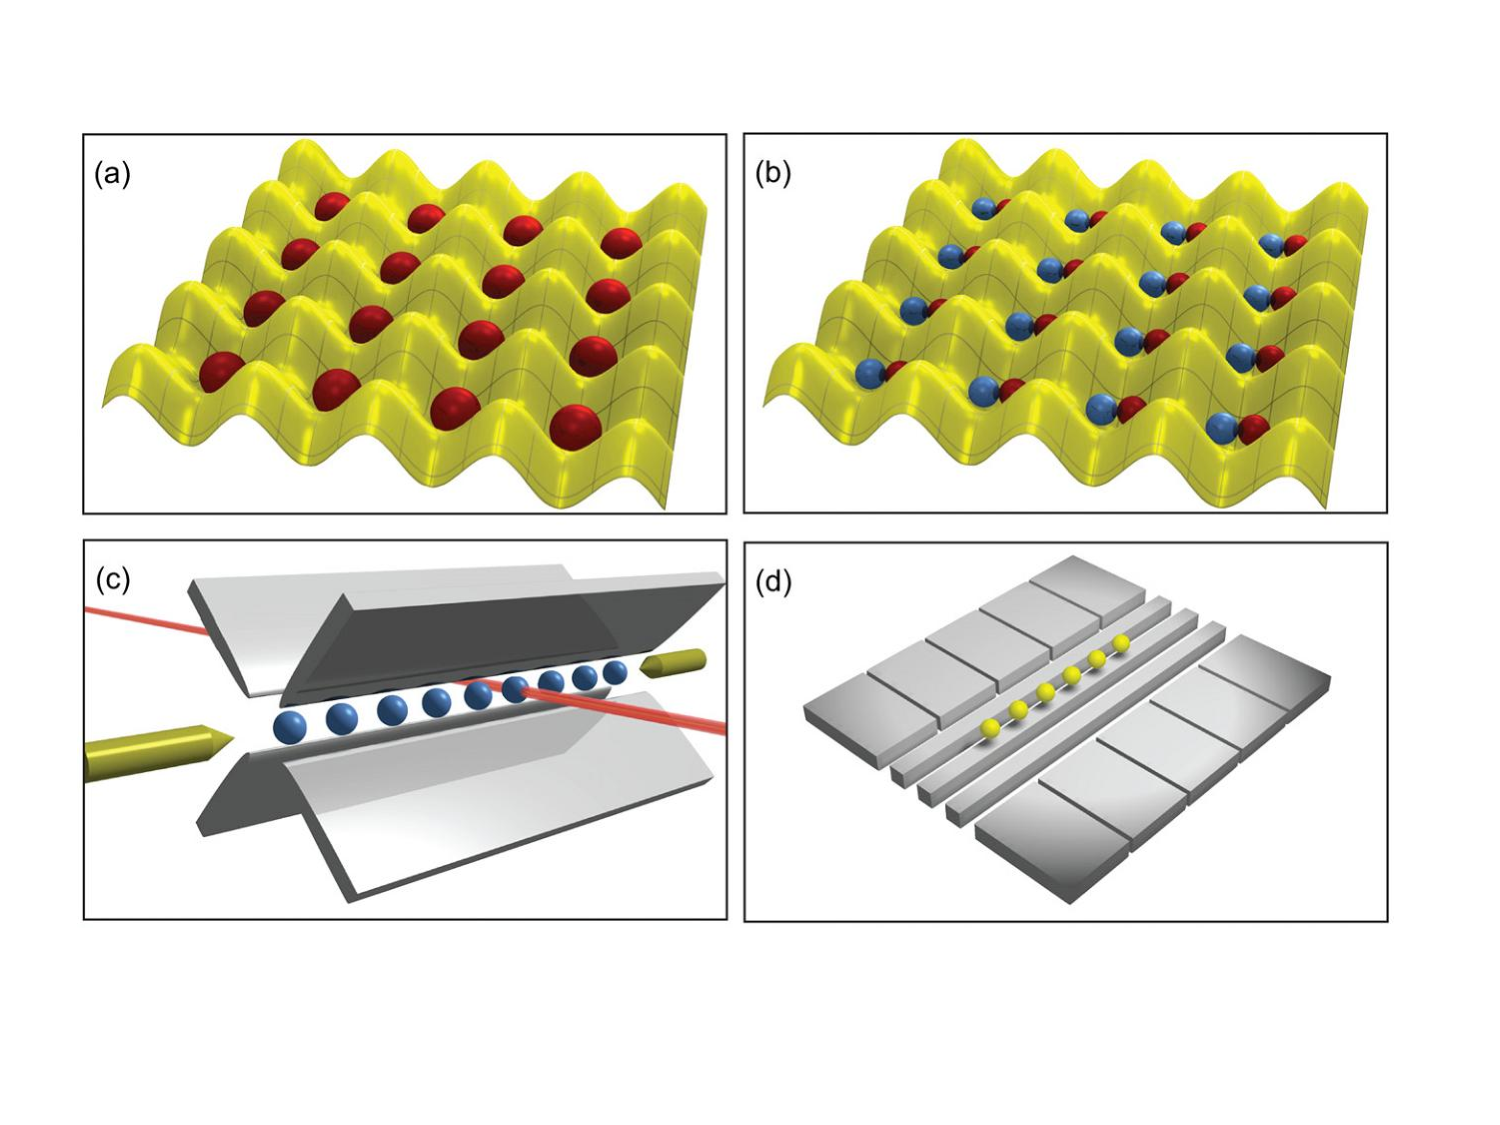
\includegraphics[width= 0.8\columnwidth]{figures/trap.pdf}
              \caption{(a)在周期光势阱中囚禁中性原子的方案。每一个中性原子是一个qubit,被囚禁在每个晶格中;(b)  可行的在中性原子中产生多粒子纠缠的方案,两个处于不同自旋态的原子束缚于同一个晶格中;(c) 线性势阱的示意图。处于同一个势阱中的离子拥有相同的振动模式,可以用来传递能量从而实现纠缠; (d) 平面势阱的示意图。近期发展的微米级离子阱技术对于在二维和三维上操控离子位置提供了相当大的便利。 取自[Rep. Prog. Phys. 74, 104401 (2011)\cite{review2}]
              }
              \label{trap}
            \end{center}
  \end{figure}

\subsection{超导线路量子计算}

超导线路典型的是$\mu$m尺度,并且是在mK温度下操作。虽然超导线路是肉眼可见的,但它依然
表现出很多可以用来作量子计算的量子行为\cite{super1,super2,super3,super4}。在超导线路中,qubit有很多种编码的方式:
在孤立的岛上超导电子的数目可以用作电压(charge) qubit;电流的方向可以用作磁通(flux) qubit;线路中的振荡态 可以用作相位(phase) qubit。这些qubit可以通过微波,电压,磁场,电流等进行高精度控制,从而实现量子计算任务。
目前超导线路中已经可以实现一些简单的量子算法\cite{super5}并产生三比特的纠缠态\cite{super6,super7,super8}。

 \begin{figure}[htbp]
            \begin{center}
              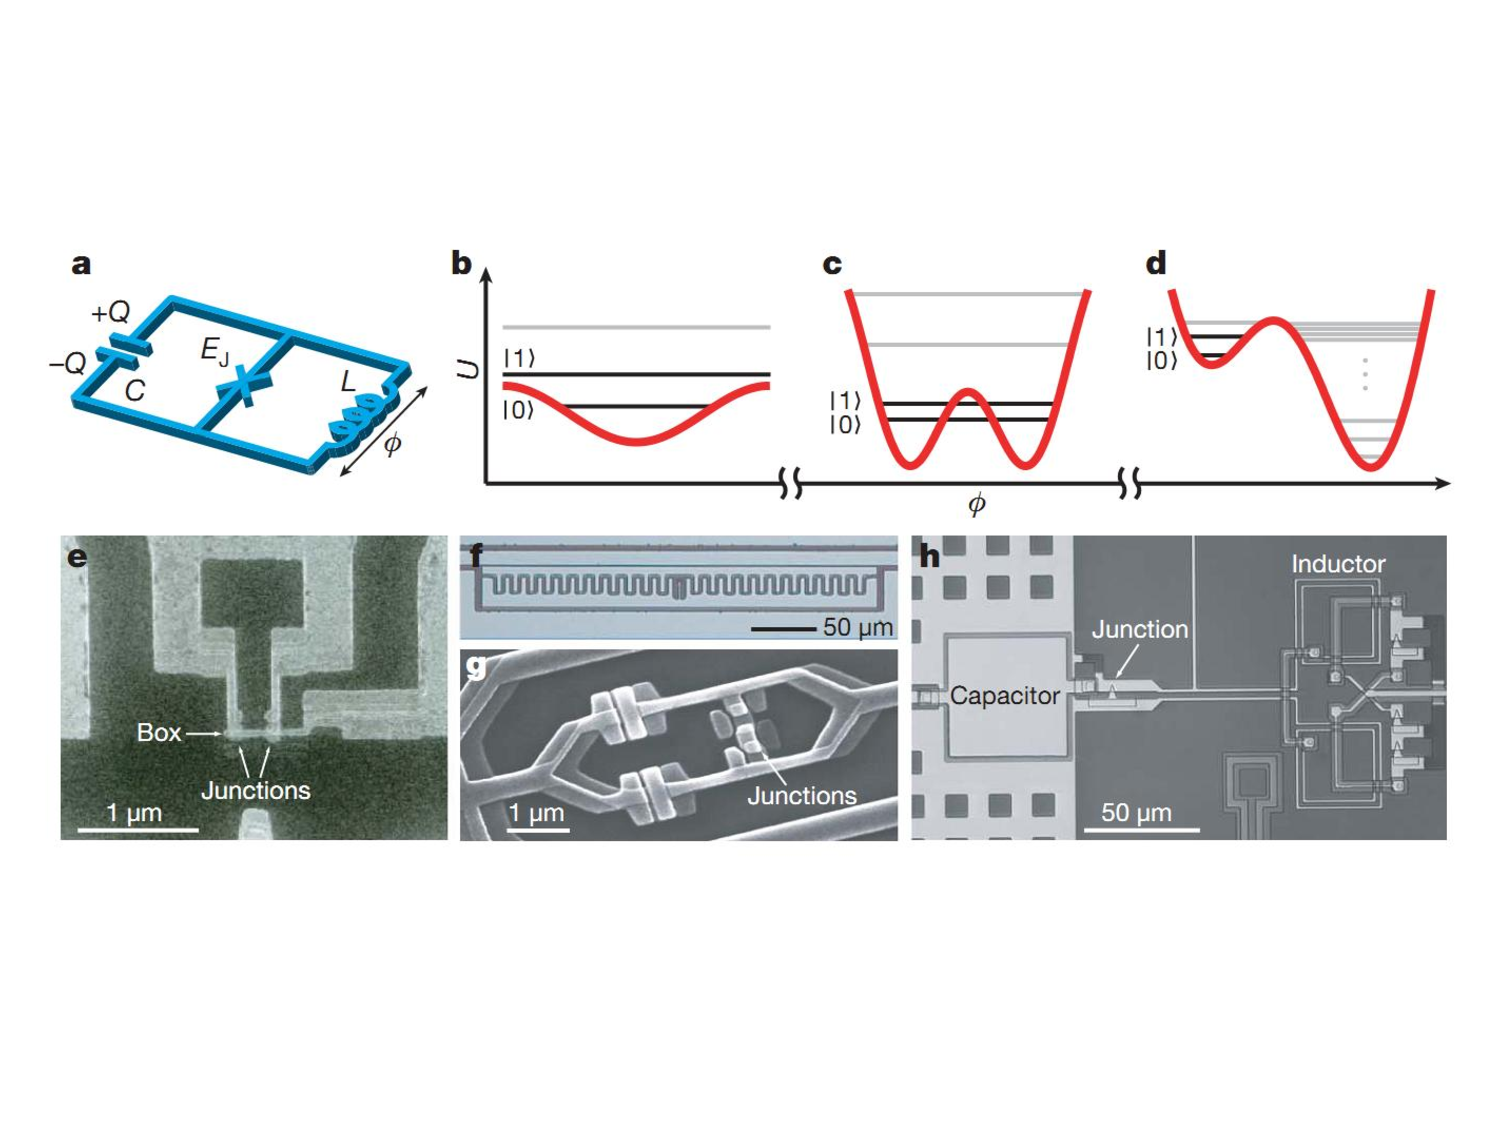
\includegraphics[width= 0.8\columnwidth]{figures/super.pdf}
              \caption{(a) 最小的超导线路模型,Josephson结用蓝色的“X”来表示;(b)-(d) Charge,flux和phase qubit中的势能(红色)以及能级(黑色);(e)-(h) 超导量子比特的微型照片。整个线路都是用铝薄膜制作的。e,f 为charge qubit,g为flux qubit,h为phase qubit。取自[Nature 464, 45 (2010)\cite{review1}]
              }
              \label{super}
            \end{center}
  \end{figure}

  \subsection{固态自旋量子计算}
当前的技术已经可以对固体中的单自旋进行相干操控和测量\cite{solid1,solid2},因此产生了
利用量子点中的电子自旋\cite{solid3}或者NV色心中的电子自旋及核自旋\cite{solid4}作量子计算的方案。
相比于其他体系,固态qubit的吸引力在于它们可以根据需要进行设计并且在大的阵列上进行扩展。
而且,固态方案要求的温度一般可以到几K的量级,NV色心更是可以在室温下进行操控。操控和读出的方法既可以
是电学手段\cite{solid5},也可以是光学手段\cite{solid6,solid7,solid8}。

虽然目前Rabi振荡已经可以在实验上被观测到\cite{solid9,solid10},但目前只有NV色心可以实现两比特门\cite{solid11},量子点中
只有一个逻辑态间的SWAP门在实验上实现了\cite{solid12}。NV色心中电子与核自旋之间纠缠起来也已在实验上实现\cite{solid13}。
\begin{figure}[htbp]
            \begin{center}
              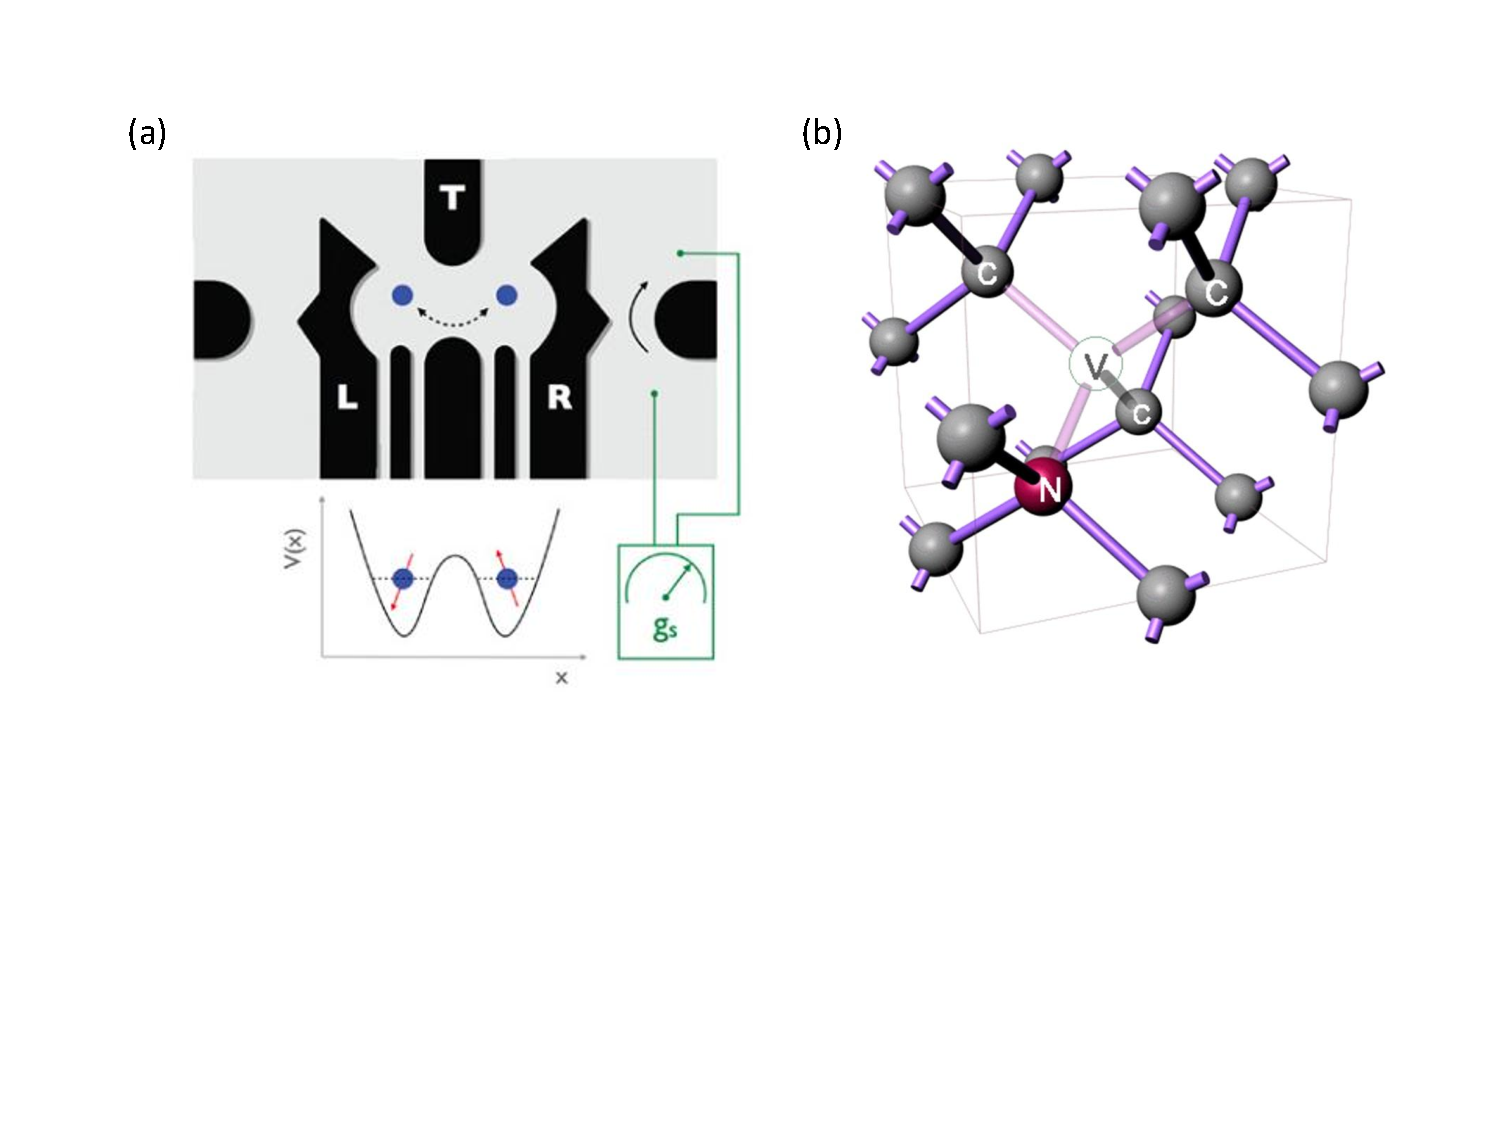
\includegraphics[width= 0.8\columnwidth]{figures/solid.pdf}
              \caption{(a) 两个电子的自旋态囚禁在半导体的双量子点结构上可以构成很好的qubit。传统的方法中,用磁场来操控qubit,但最近也发展了用电场操控的技术。取自[Rep. Prog. Phys. 74, 104401 (2011)\cite{review2}。
               (b) 金刚石中的NV色心,电子自旋可以通过磁场和可见光频率的电磁场来进行操控。取自[Phys. Rev. Lett. 93, 130501 (2004)\cite{solid11}]
              }
              \label{solid}
            \end{center}
  \end{figure}

\subsection{核磁共振量子计算}
液体溶剂中分子的核自旋非常适合做量子计算。分子的快速运动保证了该方案的$T_2$时间可以达到几秒的量级,媲美离子阱。1997年,第一次提出可以用已经存在发展了
超过50年的核磁共振技术做量子计算\cite{nmrpro1,nmrpro2}。在把样品置于核磁谱仪的强磁场中后,处于不同化学环境的核自旋可以通过Larmor进动频率分开。单比特门可以通过
外加射频脉冲实现,而两比特门可以通过核与核之间的相互作用来实现。目前,液体核磁已经可以实现最大到十二个qubit的量子计算\cite{12qubit},也已经验证了很多量子算法方案\cite{shor15}。
核磁共振遭遇的主要是可扩展性问题,想做到几十到上百个qubit理论上非常困难。
\begin{figure}[htbp]
            \begin{center}
              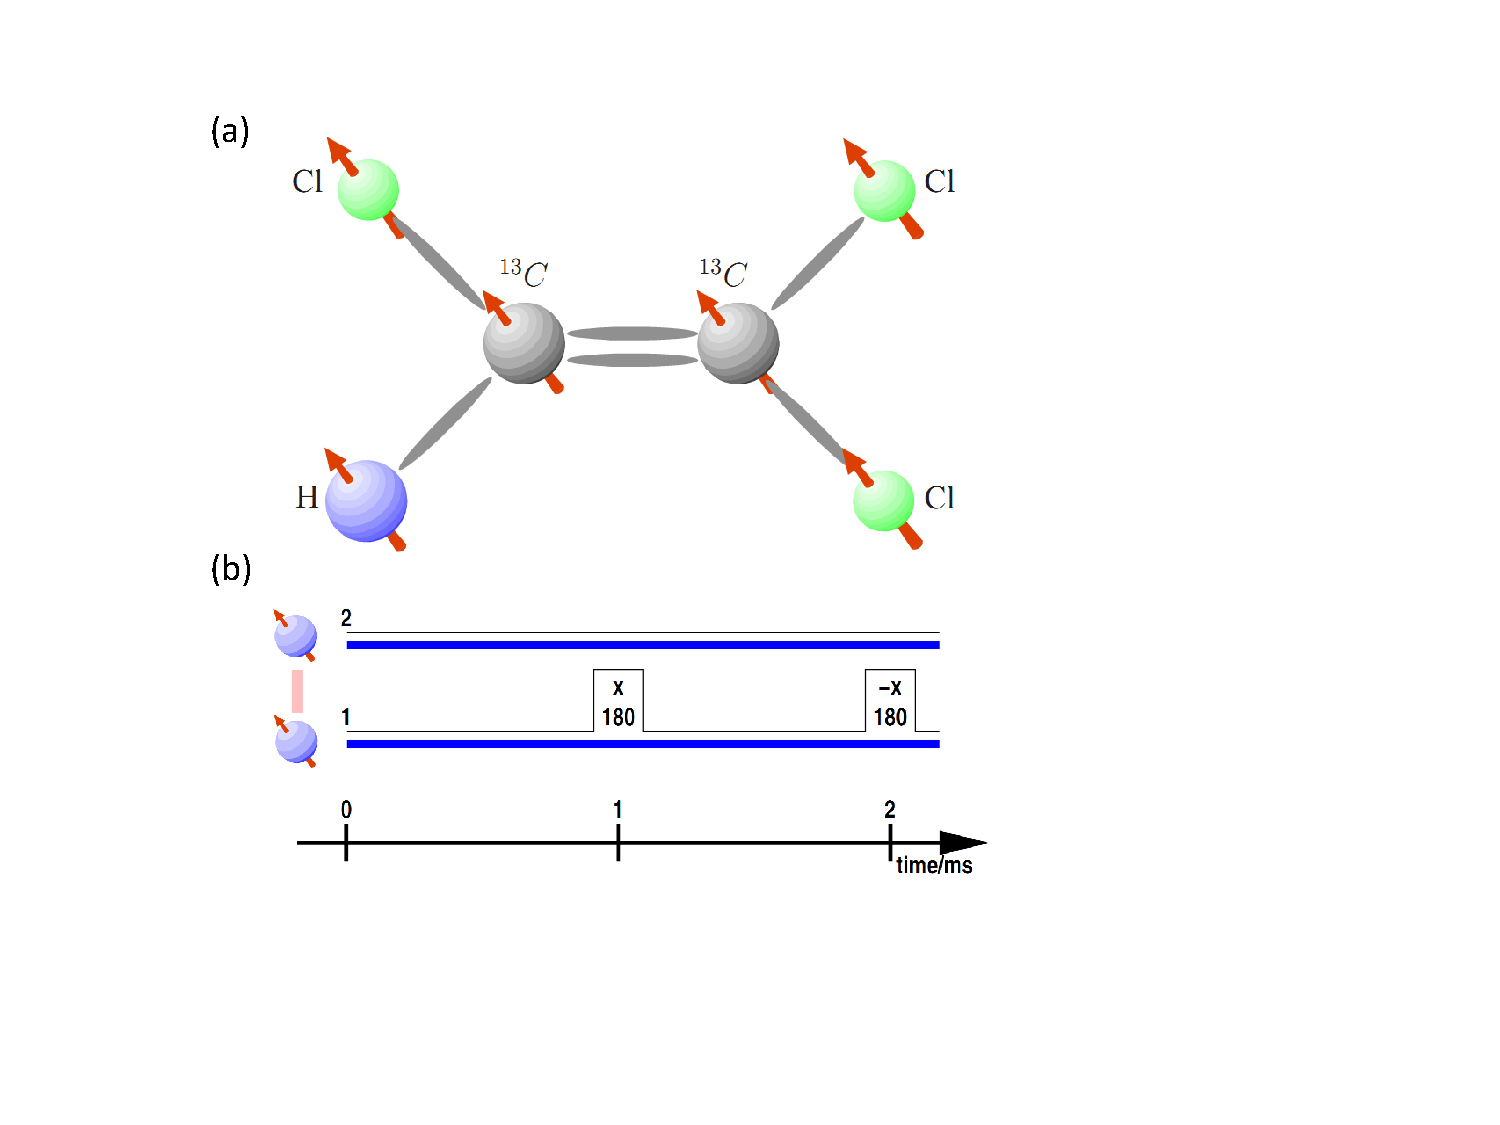
\includegraphics[width= 0.8\columnwidth]{figures/nmr.pdf}
              \caption{(a) 核磁共振中TCE分子的示意图。该分子中有三个可以用作自旋1/2的原子核,$^1$H和两个$^{13}$C。 (b)核磁共振中典型的脉冲序列示意图。该序列为耦合重聚的序列。取自[arXiv: 0207172 v1\cite{nmrreview1}]
              }
              \label{nmr}
            \end{center}
  \end{figure}

\subsection{各体系间的比较及展望}
展望未来,到底哪一个体系是最有希望实现真正的大尺度的量子计算机呢?这个问题非常难于回答,但我们首先要比较的就是各个体系的相干时间。我们给出了一个各体系之间的比较,总结于下图中。
\begin{figure}[htbp]
            \begin{center}
              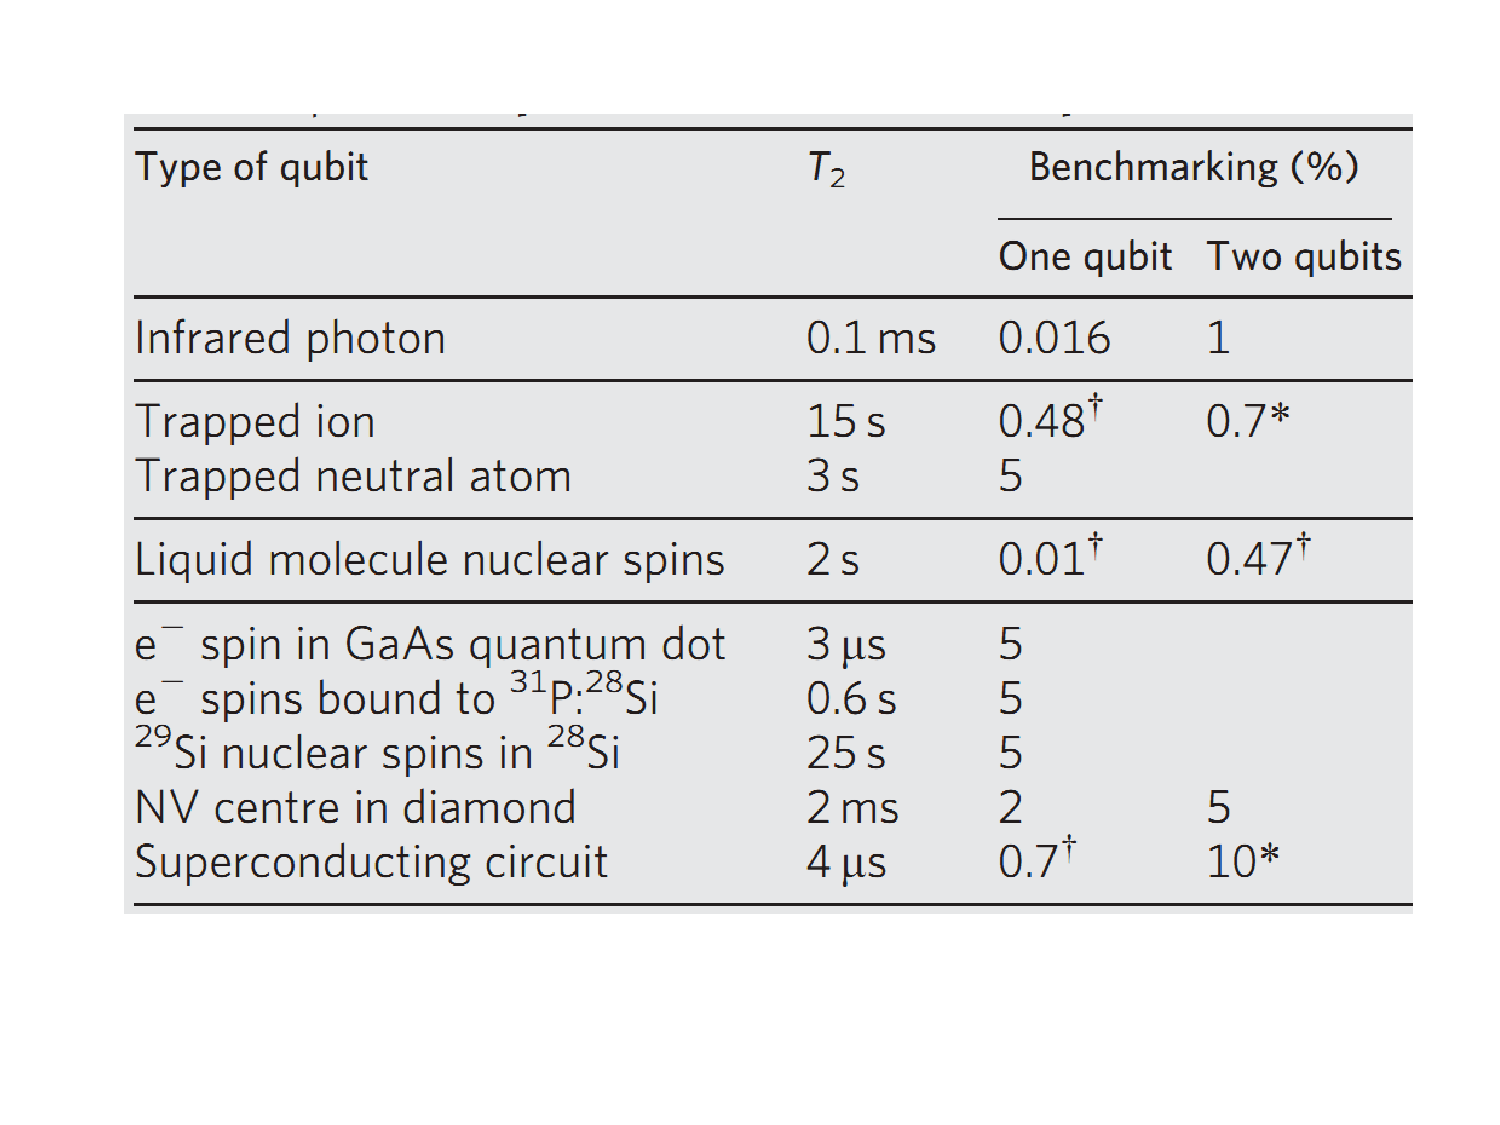
\includegraphics[width= 0.8\columnwidth]{figures/compare.pdf}
              \caption{各体系的$T_2$时间,以及逻辑门操作的保真度之间的比较。典型值给出的是单比特门和两比特门的错误概率,带$\ast$标记的数值是通过量子态重构或量子门重构得到的实验值,用100$\%$减去该值即为保真度。带$\dagger$标记的数值是通过随机基准
              (randomized benchmarking)过程获得。其他的数值则是粗略的对实验中操作误差的估计。取自[Nature 464, 45 (2010)\cite{review1}]。
              }
              \label{nmr}
            \end{center}
  \end{figure}
这些$T_2$时间可能随着技术的发展而增加,目前来看离子阱体系是最长的。当然,每个qubit的$T_2$还要和该体系的初始化,控制,以及测量时间相比较。

除了相干时间,在qubit的操控中的误差也是量子计算机必须考量的因素,这些数值也被总结在上表中。同时在逻辑门操作的时间内退相干的影响也是对逻辑门的误差有贡献的。还有各体系的量子纠错能力也是
要被考虑的因素,不过这个条件非常难以量化,它和机制复杂的噪声过程有关。

由于量子计算的实验进展是日新月异的,所以相关的参考文献最好选择最新的,比较推荐的有2010年Nature上的综述\cite{review1}以及2011年Rep. Prog. Phys.上的综述\cite{review2}。

\section{小结}

本章简略回顾了量子计算的发展历史,介绍量子计算机的工作原理以及当前实验上的进展。如果把经典计算机比喻为单一乐器的话,量子计算机就是一个交响乐团,你可以同时听到很多美妙的音乐;如果把经典计算机比喻为手动进水、漂洗、甩干的洗衣机的话,量子计算机就是
一台全自动洗衣机,只要“哔”的按下去脏衣服就一件一件变白了。但是,虽然量子计算机看上去很美好,但从目前的实验进展来看
建造一台真正的量子计算机的目标依然是很虚无缥缈的。这大概就和一个世纪前人们看待经典计算机的感觉一样。虽然很难,但我们一直在努力寻找新的方案,发展新的
技术,创造新的手段,等待所有的瓶颈都被突破的那一天。正如本章开始所说,创造一个会飞的马很难,但我们有一年的时间来努力,而一年确实是什么都有可能发生的,更何况我们用来
建造量子计算机的时间可不止一年,只要我们一直朝这个方向努力,总有一天我们会说,过去的电脑简直弱爆了,我们要玩量子并行版的Dota,我们要模拟自己的人生运势,当然闲来无事还要破解一下对门女孩子的QQ密码。

号称卖量子计算机的D-wave的广告词确实说的不错:

\emph{"Yes, you \textbf{can} have one."}


   
\chapter{量子模拟}
当1946年世界上第一台电子计算机ENIAC (Electronic Numerical Integrator And Computer) 诞生时,这个占地170平方米,重达30吨的庞然大物仅仅能在一秒中之内进行5000次加法运算,而现在富士通研发的
超级计算机K-Computer可以每秒执行8.16千万亿次浮点运算!万事开头难,在40年代总投资高达48万美元的巨款最终促使了
ENIAC的诞生,开启了一个新的时代,很难想象短短六十多年间计算机硬件已经进化到了如此的程度。

让我们转到量子计算的话题上来。其实当今量子计算的境遇和当时ENIAC诞生前很像:各国都在拨款,全世界都在竞赛,希望打赢这场新的信息战。Shor的大数分解算法和量子通信中的
BB84协议让人们认识到了量子计算机无比广阔的前景,但同时几十年来实验技术的滞后又让人们不禁泛起一丝疑虑。至少目前为止,量子计算的水平还是远远落后于经典计算的,所以人们迫切需要找到一个例子
来打败经典计算机,重拾人们的信心。

话虽如此,想做到这一点依然十分困难。如果我们从量子算法着手,比如Shor算法,我们大概需要成百上千个qubit才有希望打败经典计算,这个难度就和40年代的人妄想着建造一台
可以每秒执行千万次运算的电子计算机一样。幸好,量子计算除了量子算法这个大领域以外,还有另外一个很有影响力的领域-量子模拟。现在已经证明,利用量子模拟的手段,我们只需要30到100个qubit就可以超越经典计算!
因此,量子模拟的相关研究是实验上非常热门的领域,因为每个人都希望自己是第一个真正看到量子计算优越性的人。

本章中,我们将系统全面的介绍量子模拟这个领域,从它的历史和发展说起,阐述量子模拟的定义和分类,以及它的物理实现和在各学科的应用。当然,我们会紧跟量子模拟的
实验进展,给出未来几年量子模拟的发展前景。

\label{chap:simulation}
    \section{量子模拟理论}
    “\emph{让我们建造一台充满量子力学气息的、依循量子力学规则的新型计算机吧。}”

 \hspace{23em} \emph{--理查德·费曼}

\subsection{量子模拟的提出及发展}

其实和著名的Shor算法比起来,量子模拟的提出要早的多。

三十年前,也就是1982年,费曼就认识到如何模拟量子系统是非常有挑战性的问题\cite{Feynman2}。这个
问题根本上来说就是计算复杂度的问题:随着量子体系维度的增长,为了存储量子态所需的经典寄存器是指数增加的。不仅如此,模拟量子系统的演化也需要指数增长的逻辑门操作。
这种“指数爆炸”困难是不可回避的,除非用一些经典随机或近似方法,例如Monte Carlo方法,平均场理论,密度泛函理论及格林函数方法等。但遗憾的是这些方法并不总是有效的,而且还面临许多限制。为了多存储一个自旋1/2的粒子,经典计算的存储空间就要
加倍,毫无疑问即使对于今日的超级计算机来说模拟量子系统依然是非常头痛的。

上述问题的可能的解决方案也是费曼在同一篇文章中提出:利用基于量子力学规则建造的新型计算机应该可以\cite{Feynman2}。在费曼的文章中并没有涉及具体的要用到
什么函数或者什么手段,他只是猜测这种计算机应该是可以有效解决这类问题的。十多年后,Lloyd终于证明一台量子计算机是可以作为普适的量子模拟器,来模拟这些问题的\cite{Lloyd}。当然,针对某些特殊的问题
有时并不需要一台真正的量子计算机,一些简单的设备也是有可能模拟需求的问题的(当然这些肯定不是普适的量子模拟器)。

最近量子模拟变得热门主要是两个方面的原因。第一,理论上很多学科的问题,只要牵涉到量子行为,都可以通过量子模拟来解决。不仅仅是物理领域,化学、生物、材料学等看似毫不相干的学科中
也已经诞生了很多量子模拟的方案。比如在凝聚态物理中,量子模拟就可以用来研究量子相变,量子磁体,高温超导等。还有高能物理,计算量子化学,甚至宇宙学等等众多有影响力的领域都能
和量子模拟扯上关系。第二,目前实验上的相干控制技术已经足以给出一些演示性的实验来验证量子模拟理论,而且很多研究组也已经在研究十个qubit以上的量子模拟器。实验上的代表性工作参见文献\cite{ionphase,mott,dirac,optics_static},
这些工作也将在后面的部分详细叙述。有了这些漂亮的实验,人们有理由相信未来的几年内量子模拟会取得突破性进展的,超越经典也不是不可能完成的任务。

\begin{figure}[htbp]
            \begin{center}
              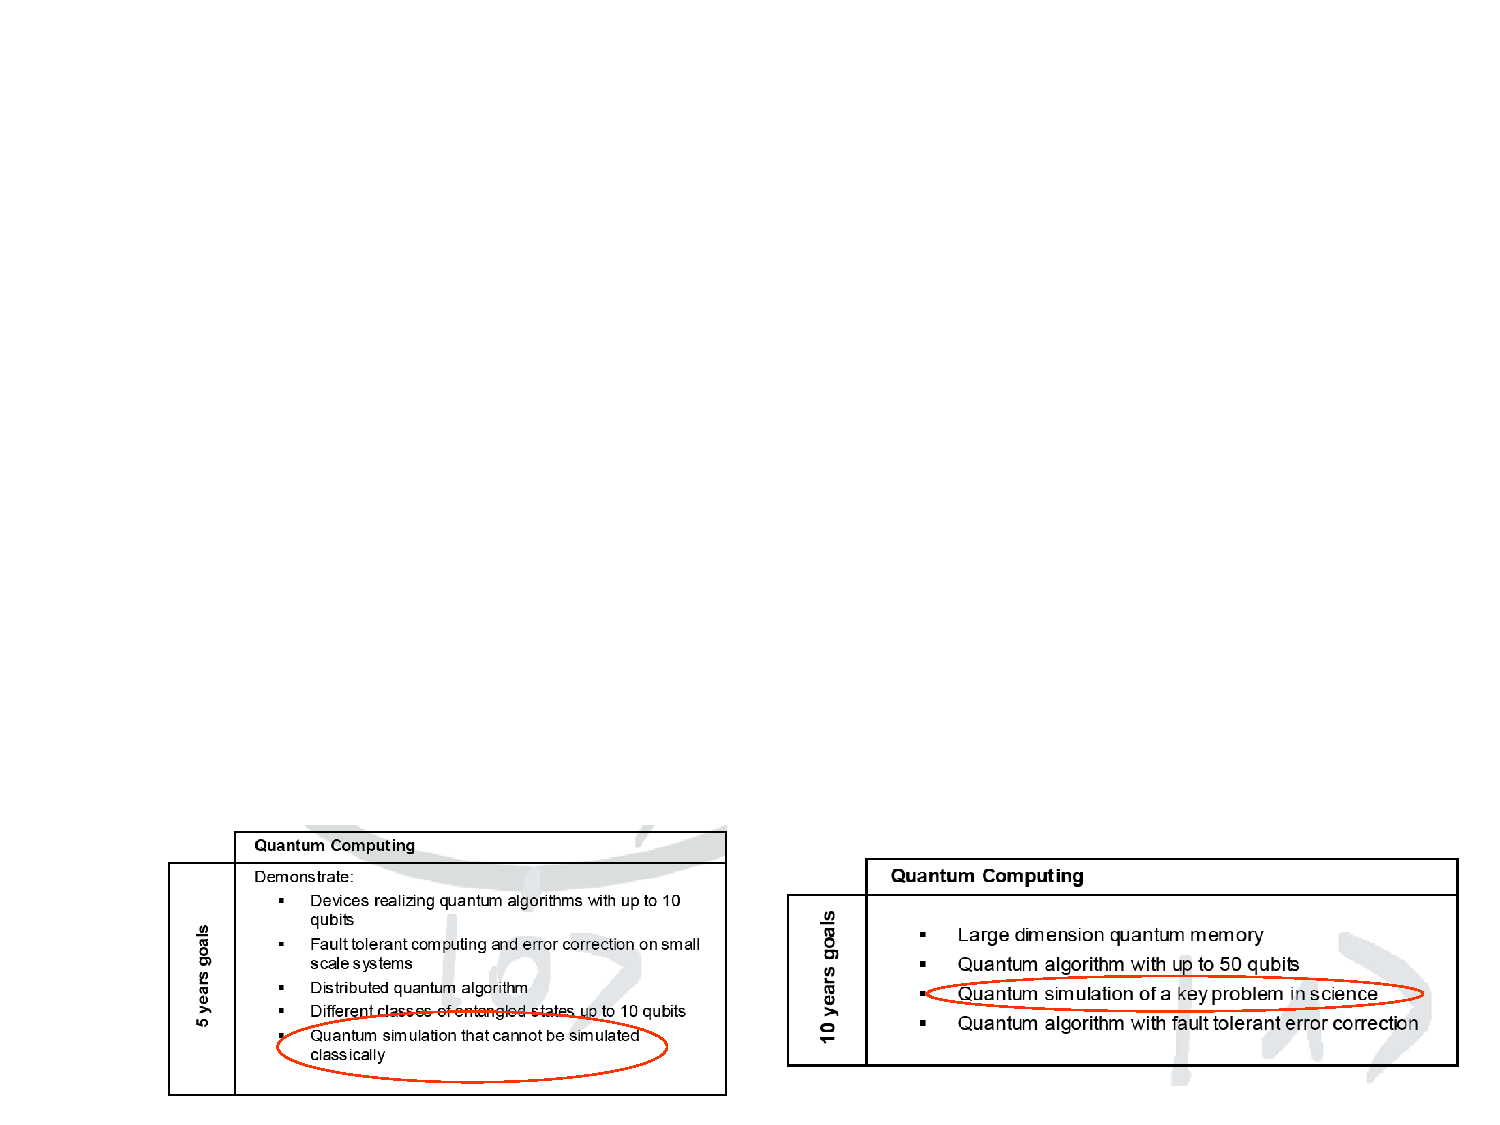
\includegraphics[width= 0.8\columnwidth]{figures/eu.pdf}
              \caption{在2008年欧盟关于量子计算的战略规划中,计划五年之内量子模拟上要找到一个超越经典的例子,而十年内量子模拟要成为科学研究上的一个关键问题。现在距离五年目标它们还剩一年。
              }
              \label{eu}
            \end{center}
        \end{figure}


\subsection{量子模拟的定义}

我们这里给出一个并不十分严格的量子模拟的定义:

   “\emph{量子模拟就是用量子力学的方法来模拟量子系统。}”

也就是说,我们可以通过一个可控的量子系统来模拟其他量子系统\cite{simreview}。假设要模拟的系统的量子态为$\left\vert \phi \right\rangle$,该系统经过幺正演化
\begin{equation}
          U = e^{-iH_{sys}t}
 \end{equation}
从初态$\left\vert \phi(0) \right\rangle$演化到了$\left\vert \phi(t) \right\rangle$。其中,$H_{sys}$是系统的哈密顿量。而量子模拟器中作为一个可控的量子系统,其初态为
$\left\vert \psi(0) \right\rangle$,演化算子为
\begin{equation}
          U' = e^{-iH_{sim}t}.
 \end{equation}
 这里$H_{sim}$是模拟器的哈密顿量,而经过该演化后,模拟器的末态变为$\left\vert \psi(t) \right\rangle$,并且这个态是容易测量的。如果在这两个量子系统间存在一个映射,即$\left\vert \phi(0) \right\rangle$和$\left\vert \psi(0) \right\rangle$,$\left\vert \phi(t) \right\rangle$和$\left\vert \psi(t) \right\rangle$之间存在映射关系,
 那么原量子系统就可以被模拟,其表示可以见图\ref{schematic}。
        \begin{figure}[htbp]
            \begin{center}
              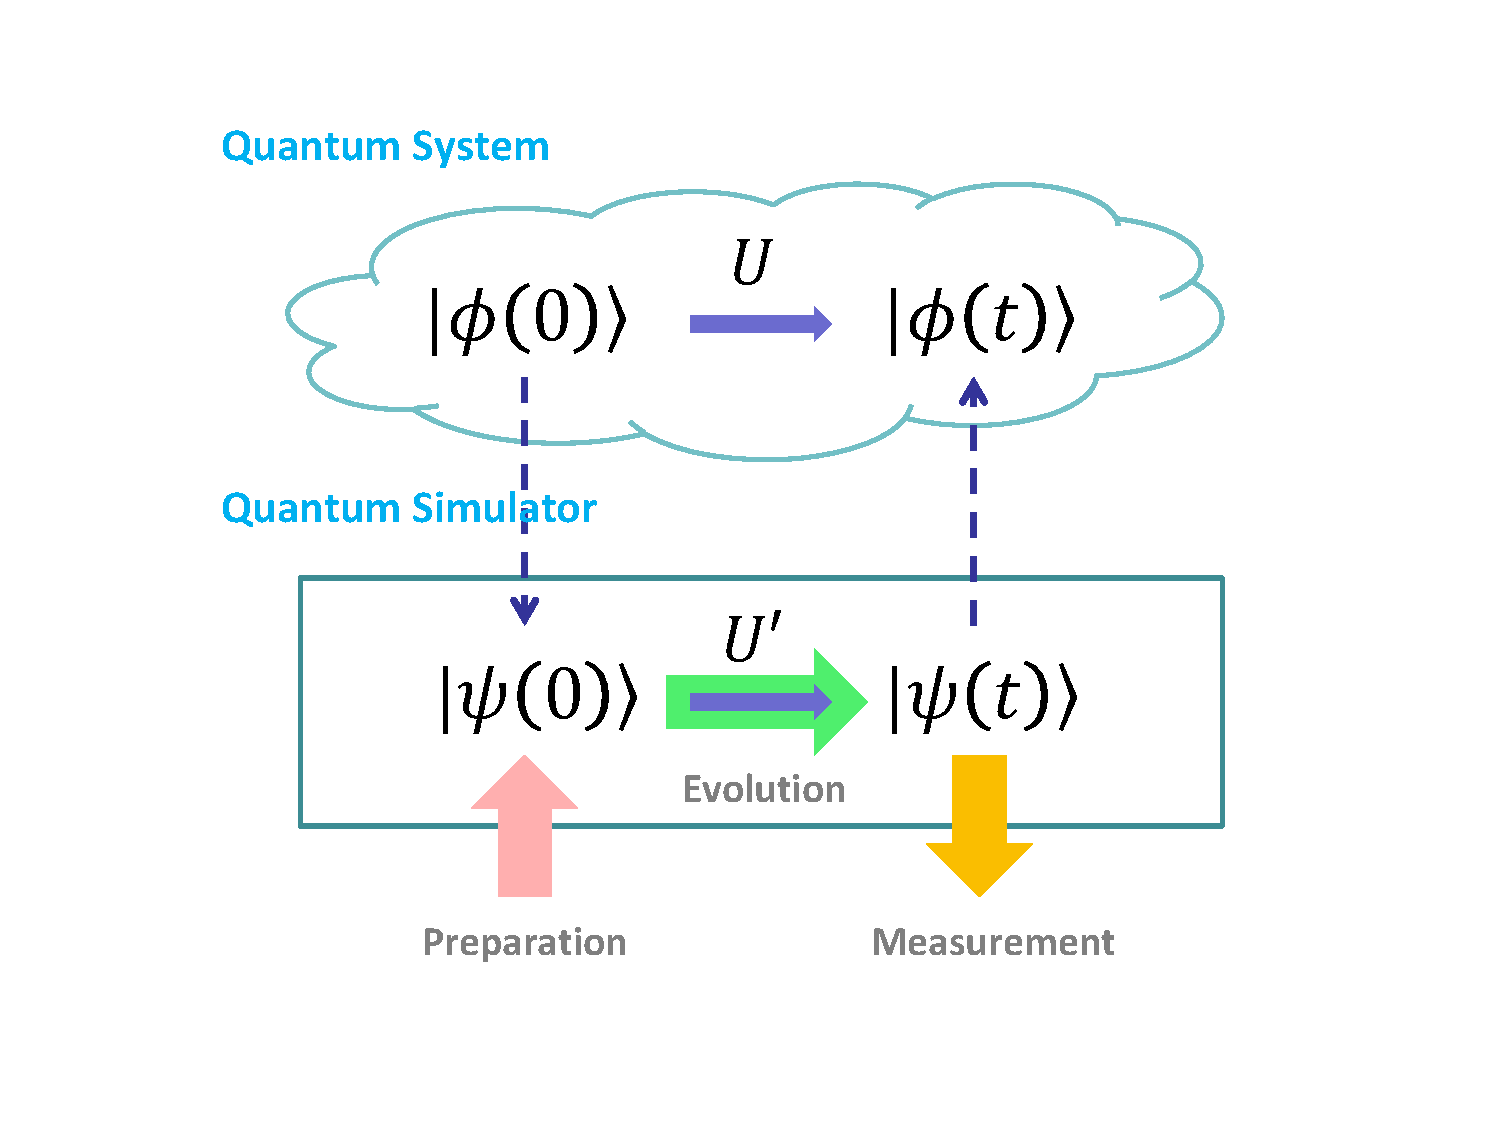
\includegraphics[width= 0.8\columnwidth]{figures/schematic.pdf}
              \caption{量子模拟过程的示意图。量子系统从$\left\vert \phi(0) \right\rangle$经过$U = e^{-iH_{sys}t}$演化到了$\left\vert \phi(t) \right\rangle$,量子模拟器则从$\left\vert \psi(0) \right\rangle$经过$U' = e^{-iH_{sim}t}$演化到$\left\vert \psi(t) \right\rangle$。同时,$\left\vert \phi(0) \right\rangle$和$\left\vert \psi(0) \right\rangle$,$\left\vert \phi(t) \right\rangle$和$\left\vert \psi(t) \right\rangle$之间存在映射关系。虽然量子系统本身不可控制(或者实验上很难控制),但量子模拟器是可以轻易操控的,或者说,初态$\left\vert \psi(0) \right\rangle$容易制备,演化$U'$容易控制,末态$\left\vert \psi(t) \right\rangle$容易测量。有颜色的箭头表示是可控操作。
              }
              \label{schematic}
            \end{center}
        \end{figure}

量子模拟主要分为两类,数字量子模拟(digital quantum simulation, DQS)和类比量子模拟(analog quantum simulation, AQS),这两个概念非常类似于电子学中的数字电路和模拟电路的概念,下面就分别介绍这两种量子模拟形式。

\subsection{数字量子模拟}

为了得到模拟器的末态,我们必须把一个幺正操作作用到初态上,即
\begin{equation}
         \left\vert \psi(t) \right\rangle = U\left\vert \psi(0) \right\rangle  = e^{-iHt}\left\vert \psi(0) \right\rangle.
 \end{equation}
由于$U$可能是多比特的非常复杂的操作,我们一般会用近似把其展开成多个指数项$e^{-iH_lt}$的乘积,其中$H_l$是哈密顿量中的局域相互作用(当然前提是该哈密顿量可以写成
一系列的局域哈密顿量的和的形式)。然后,我们可以利用单比特旋转门和两比特CNOT门把整个$U$展开,就可以得到末态$\left\vert \psi(t) \right\rangle$,从而实现量子模拟任务。这种模拟形式和基于门的量子计算非常类似,也被称作“\textbf{数字量子模拟}”。

理论上,任何的幺正操作总可以用一系列的逻辑门展开,因此原则上来说任何操作都可以被模拟,也就是数字量子模拟是普适的。但实际情况是,并不是所有的幺正操作都可以
有效展开的(仅消耗多项式资源),而且有效拆解逻辑门本身就是一个困难的问题。另外一个问题是,$U$的分解是通过近似方式得到的,所以为了得到高精度的结果,我们必须采用更高阶的近似公式,但
这样做会让逻辑门的个数大量增加。

一般来说,DQS的过程分为以下三步:初态制备,幺正演化及测量读出。下面我们将详细讨论这三个步骤\cite{brown}。

\emph{1. 初态制备}

DQS的第一步就是把量子寄存器从$\left\vert 000\ldots \right\rangle$态上制备到$\left\vert \psi(0) \right\rangle$上。在大多数情况下寻找一个有效的算法是非常困难的,只有一些特定的问题可以做到有效制备初态,比如从一个非对称态出发,可以通过多项式资源
制备到反对称的$n!$个叠加态\cite{ini1};制备$N$个粒子的费米态
\begin{equation}
         \left\vert \psi(0) \right\rangle = \prod_{j=1}^N b_j^{\dagger}\left\vert v \right\rangle,
 \end{equation}
其中$\left\vert v \right\rangle$是真空态,$b_j^{\dagger}$是费米算子\cite{ini2,ini3};有效制备常用的化学波函数\cite{Polynomial_time_algorithm};利用占据$n$个自旋轨道的$m$个电子有效制备分子系统的纯态\cite{ini4}
等等。

        \begin{figure}[htbp]
            \begin{center}
              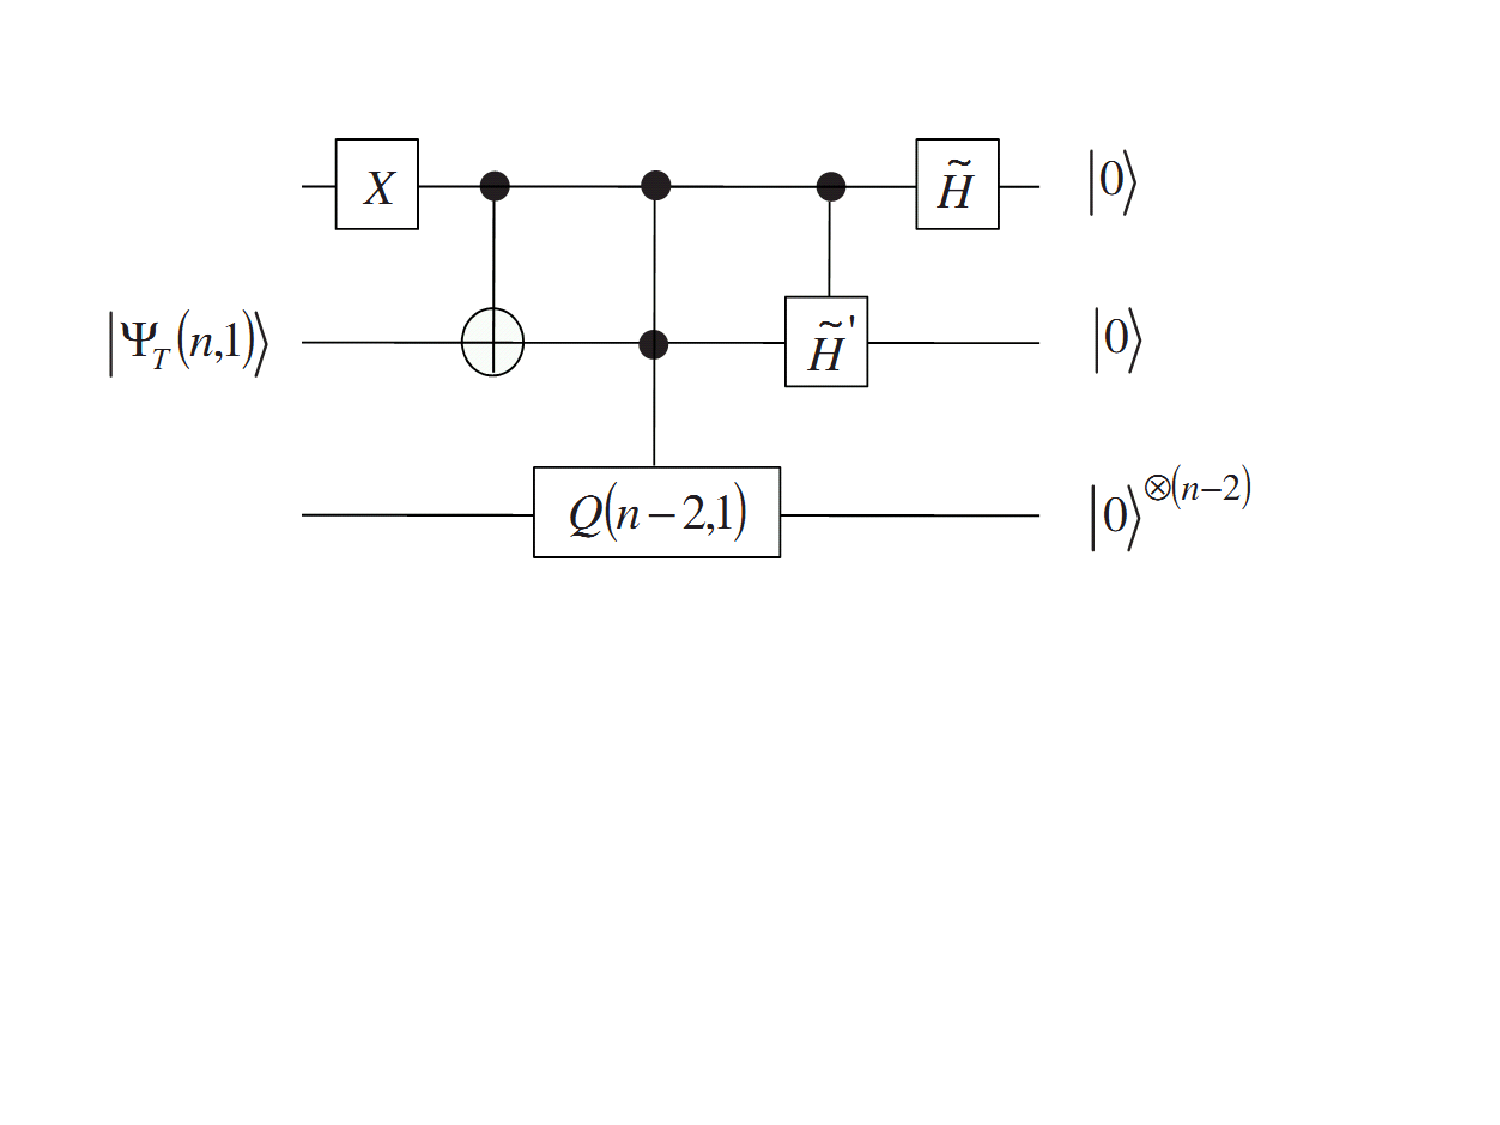
\includegraphics[width= 0.8\columnwidth]{figures/initial.pdf}
              \caption{和一般的初态制备不同,这里的方法是把目标态制备到初态。取自[Phys. Rev. A 79, 042335 (2009)\cite{ini4}
]
              }
              \label{schematic}
            \end{center}
        \end{figure}

\emph{2. 幺正演化}

假设DQS的哈密顿量可以写成一系列局域哈密顿量的和
\begin{equation}
         H = \sum_{l=1}^MH_l,
 \end{equation}
 比如Hubbard和Ising模型的哈密顿量就是这种形式。如果对所有的$l$和$l'$,满足$[H_l, H_{l'}]=0$,那么有
 \begin{equation}
         U = \prod_l e^{-iH_lt}.
 \end{equation}
 否则我们需要用一些近似手段,比如著名的Trotter-Suzuki公式\cite{trotter}
 \begin{equation}\label{trotter}
 U(\delta t)  = \prod\limits_{l=1}^M e^{-iH_l\delta t}+\mathcal {O}(\delta t^2).
\end{equation}
当$\delta t$ 趋近于0时,
 \begin{equation}\label{trotter}
 U(\delta t) \approx  \prod\limits_{l=1}^M e^{-iH_l\delta t}.
\end{equation}
这种方法的缺点是高精度依赖于很小的$\delta t$ ,那么也就会产生大量的逻辑门。目前也有很多文献重新强调Trotter-Suzuki公式的缺点\cite{tro1,tro2}。

\emph{3. 测量读出}

在得到末态$\left\vert \psi(t) \right\rangle = U\left\vert \psi(0) \right\rangle$后,我们必须进行测量来得到需要的信息。一般来说最常用的是量子态重构(tomography)技术,但它并不是可扩展的,所要求的资源也是随着体系的增大
而指数增加的。为了避免这个问题,也有一些方案提出可以利用通过测量特定的物理参数得到想要的信息,比如相关函数或算符谱\cite{ini2},当然这些方法并不是普适的。

比如,为了测量期望值$\langle U^{\dagger}V\rangle$,我们可以通过下图(a)中的线路来实现\cite{mea1}。把一个辅助比特制备到$\left\vert + \right\rangle=(\left\vert 0 \right\rangle+\left\vert 1 \right\rangle)/\sqrt{2}$后,通过网络图演化后我们只需要测量辅助位的期望值$\langle 2\sigma_{+}^a \rangle$就可以得到想要的结果。第二个例子是
描述如何测量一个厄米算符$\hat{Q}$的谱,我们依然可以通过添加辅助位$\left\vert + \right\rangle=(\left\vert 0 \right\rangle+\left\vert 1 \right\rangle)/\sqrt{2}$,并测量辅助位的期望值来实现。

        \begin{figure}[htbp]
            \begin{center}
              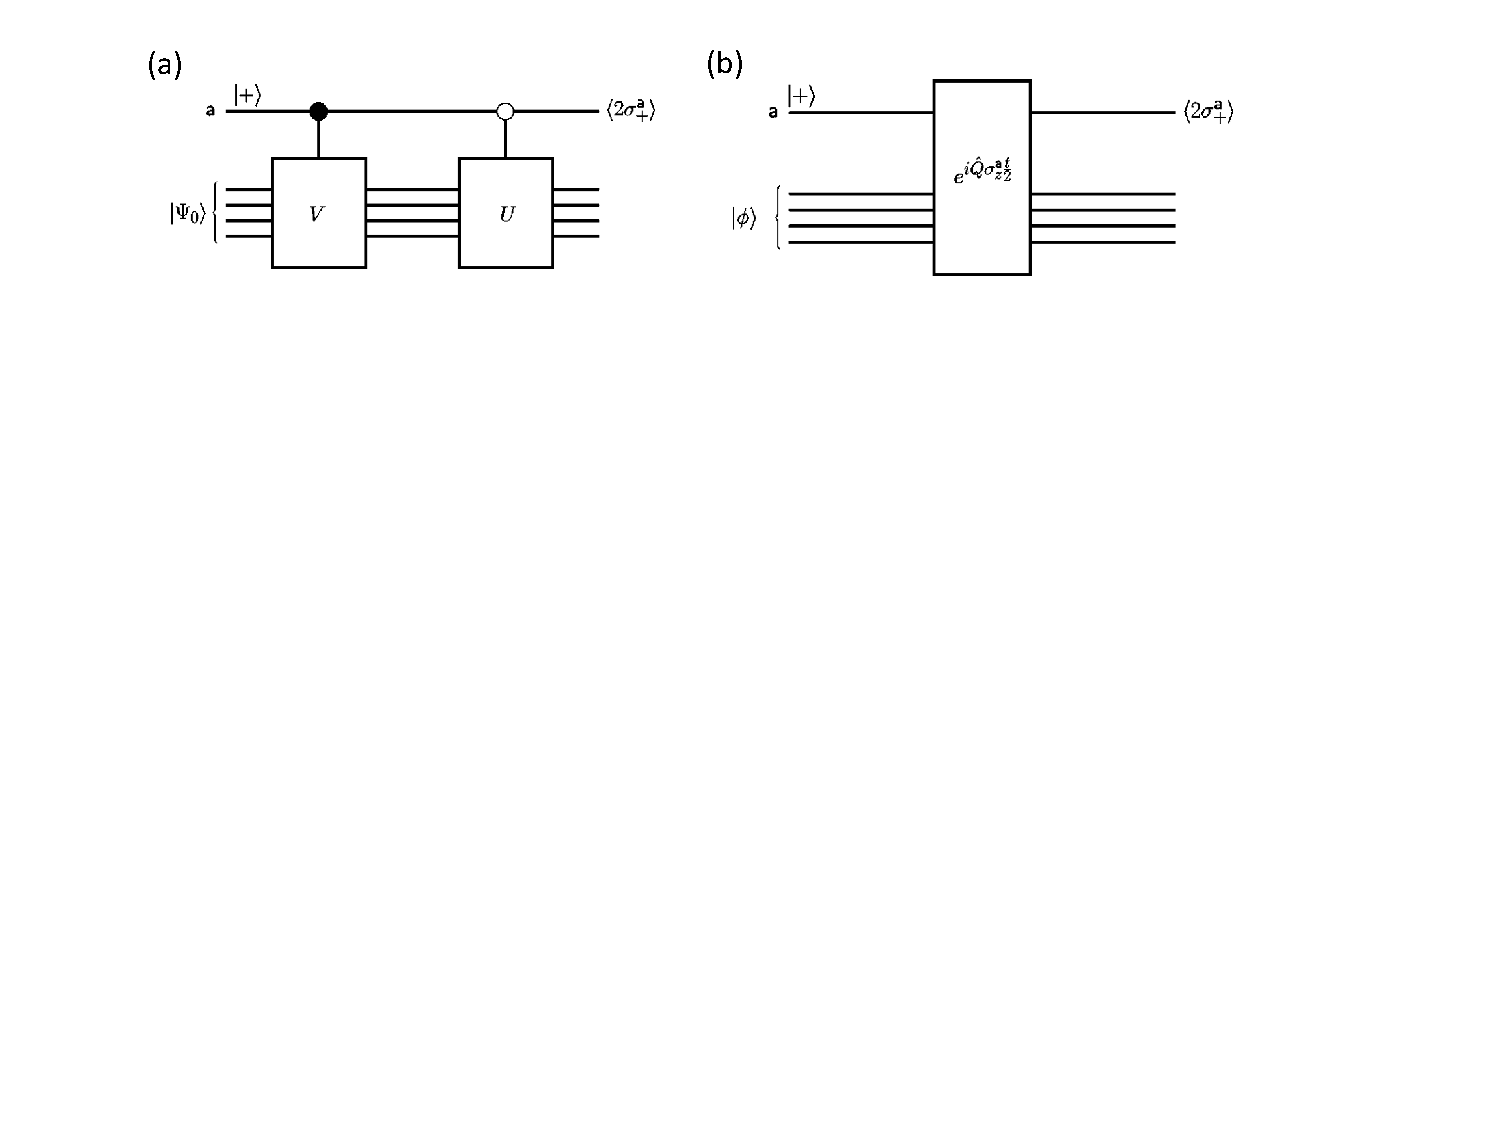
\includegraphics[width= 0.8\columnwidth]{figures/measure.pdf}
              \caption{(a) 测量期望值$\langle U^{\dagger}V\rangle$的线路图。辅助比特制备到$\left\vert + \right\rangle=(\left\vert 0 \right\rangle+\left\vert 1 \right\rangle)/\sqrt{2}$。(b) 测量厄米算符$\hat{Q}$的谱的线路图。取自[Phys. Rev. A 65, 042323 (2002)\cite{mea1}]
              }
              \label{measure}
            \end{center}
        \end{figure}

\subsection{类比量子模拟}

另外一个模拟量子系统的途径就是用类比的方法,也就是“\textbf{类比量子模拟}”。被模拟系统的哈密顿量$H_{sys}$直接映射到模拟器的哈密顿量$H_{sim}$上,也就是
 \begin{equation}\label{trotter}
 H_{sys}\longleftrightarrow H_{sim}.
\end{equation}
一般来说,只有两个量子系统非常相似的时候才能用类比的方法,所以它不是普适的,AQS的模拟精度取决于模拟器重现被模拟系统的演化过程的程度。
尽管不是普适的,AQS吸引人的地方在于它的物理要求较小,并容易在实验上实现。

寻找合适的映射是AQS的核心。一眼看上去,这个过程仿佛要比拆解逻辑门简单许多,但其实两者都很困难。如果模拟器和被模拟系统非常相近,当然AQS的实现会非常直观,遗憾的是
大多数情况并不是这么理想。简单的例子比如描述晶格势场中玻色气体(boson gas)的哈密顿量形式是
 \begin{equation}\label{trotter}
 H_{sim} = -J\sum_{i,j}\hat{a}_i^{\dagger} \hat{a}_j+\sum_i\epsilon_i \hat{n}_i+\frac{1}{2}U\sum_i\hat{n}_i(\hat{n}_i-1),
\end{equation}
其中$\hat{a}_i^{\dagger}$和$\hat{a}_i$对应于第$i$个晶格上的产生和湮灭算符,$\epsilon_i$是第$i$个晶格上由于原子的外部谐振限制产生的能量偏移。$U$是处于单个晶格上
的两个原子间的互斥作用。该哈密顿量模型的形式正好对应于Bose-Hubbard模型
 \begin{equation}\label{trotter}
 H_{BH} = -J\sum_{i,j}(\hat{b}_i^{\dagger} \hat{b}_j+h.c.)-\mu\sum_i \hat{n}_i+\frac{1}{2}U\sum_i\hat{n}_i(\hat{n}_i-1).
\end{equation}
因此这两个系统之间的类比模拟是非常直接的,但是大多数情况下就没这么直观了。

AQS中的初态制备和测量读出至今没有文献进行过详尽讨论。这是因为我们已经假设被模拟体系和模拟器之间已经非常相似,那么初态制备应该是可以有效实现的。同时,
测量模拟器的某些物理参量也可以得到被模拟系统的信息。尽管如此,AQS中的初态制备和测量读出过程依然是以后值得研究的问题。

下图是一个关于DQS和AQS之间的比较:

        \begin{figure}[htbp]
            \begin{center}
              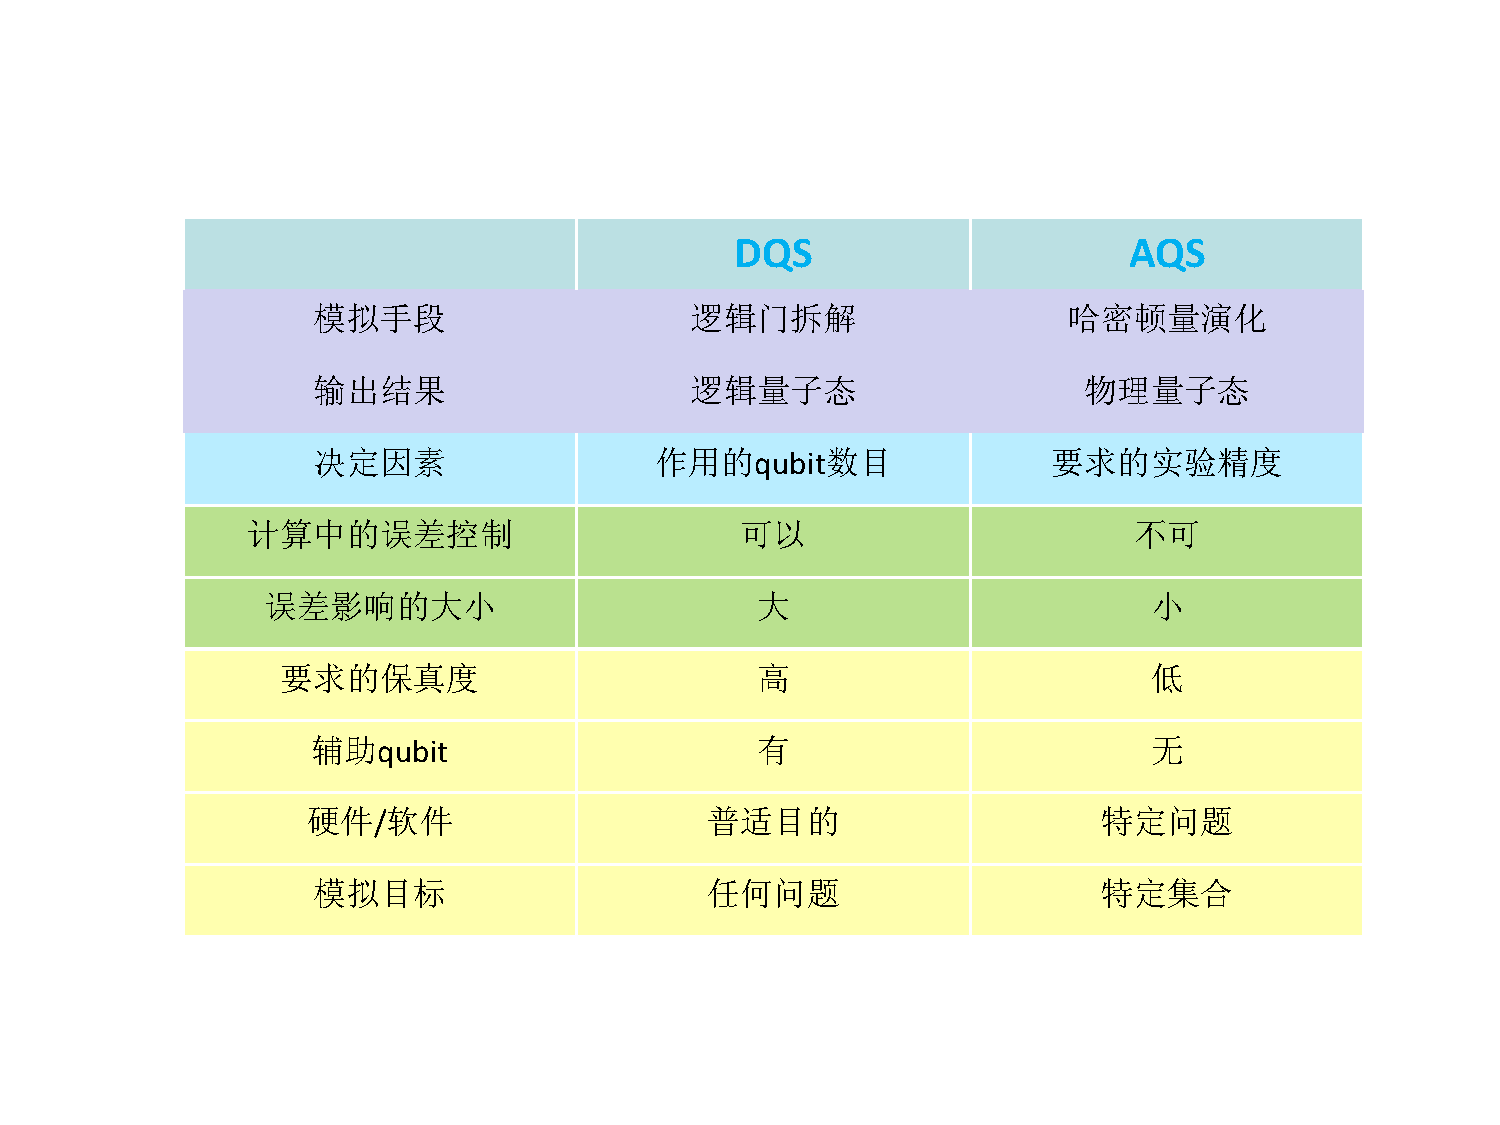
\includegraphics[width= 0.8\columnwidth]{figures/dqsaqs.pdf}
              \caption{DQS和AQS之间的比较。
              }
              \label{dqsaqs}
            \end{center}
        \end{figure}

\subsection{量子模拟的资源要求}

为了实现有效的量子模拟我们到底需要多少个qubit?这个问题的答案依被模拟对象的不同而不同。一般来说AQS对qubit的数目需求较少,当然DQS中也存在一些只用几十个甚至几个qubit
就能解决的问题。例如,在少于十个qubit的情况下,我们可以模拟量子混沌\cite{chaos1,chaos2},化学反应\cite{reaction},Dirac粒子\cite{dirac1,dirac2,dirac},Unruh效应\cite{unruh},任意子\cite{anyons1,anyons2}等等。
而用十几个qubit,我们可以模拟自旋玻璃\cite{glass1,glass2}或者分子能级\cite{Alan_first}。现在认为要超越经典计算的话我们只需要30-100个qubit的量子模拟器\cite{Alan_first}。

一般来说,DQS需要的资源和操控都要高于AQS。而且在DQS中,提高精度的代价是指数增长的逻辑操作\cite{tro1}。不过量子模拟的优势之一就是不需要很高的精度,所以这依然是可以达成的。

我们举一个量子模拟对资源要求的例子:模拟通过双势阱进行相互作用的N个粒子\cite{Polynomial_time_algorithm}。对每个自由度,该模拟都需要$n$个qubit,每个辅助位则需要$m$个qubit,而为了模拟Coulomb势场,又需要4个辅助位。
所以我们一共需要$n(3N-6)+4m$个qubit。Coulomb势场可以用$O(N^2m^2)$步来模拟,因此这个化学反应过程可以用$O(N^2m^2)$模拟,比起经典计算机这已经是指数加速了。
但另一方面来看,为了超越经典计算机我们需要至少100个qubit和200,000个逻辑门!

        \begin{figure}[htbp]
            \begin{center}
              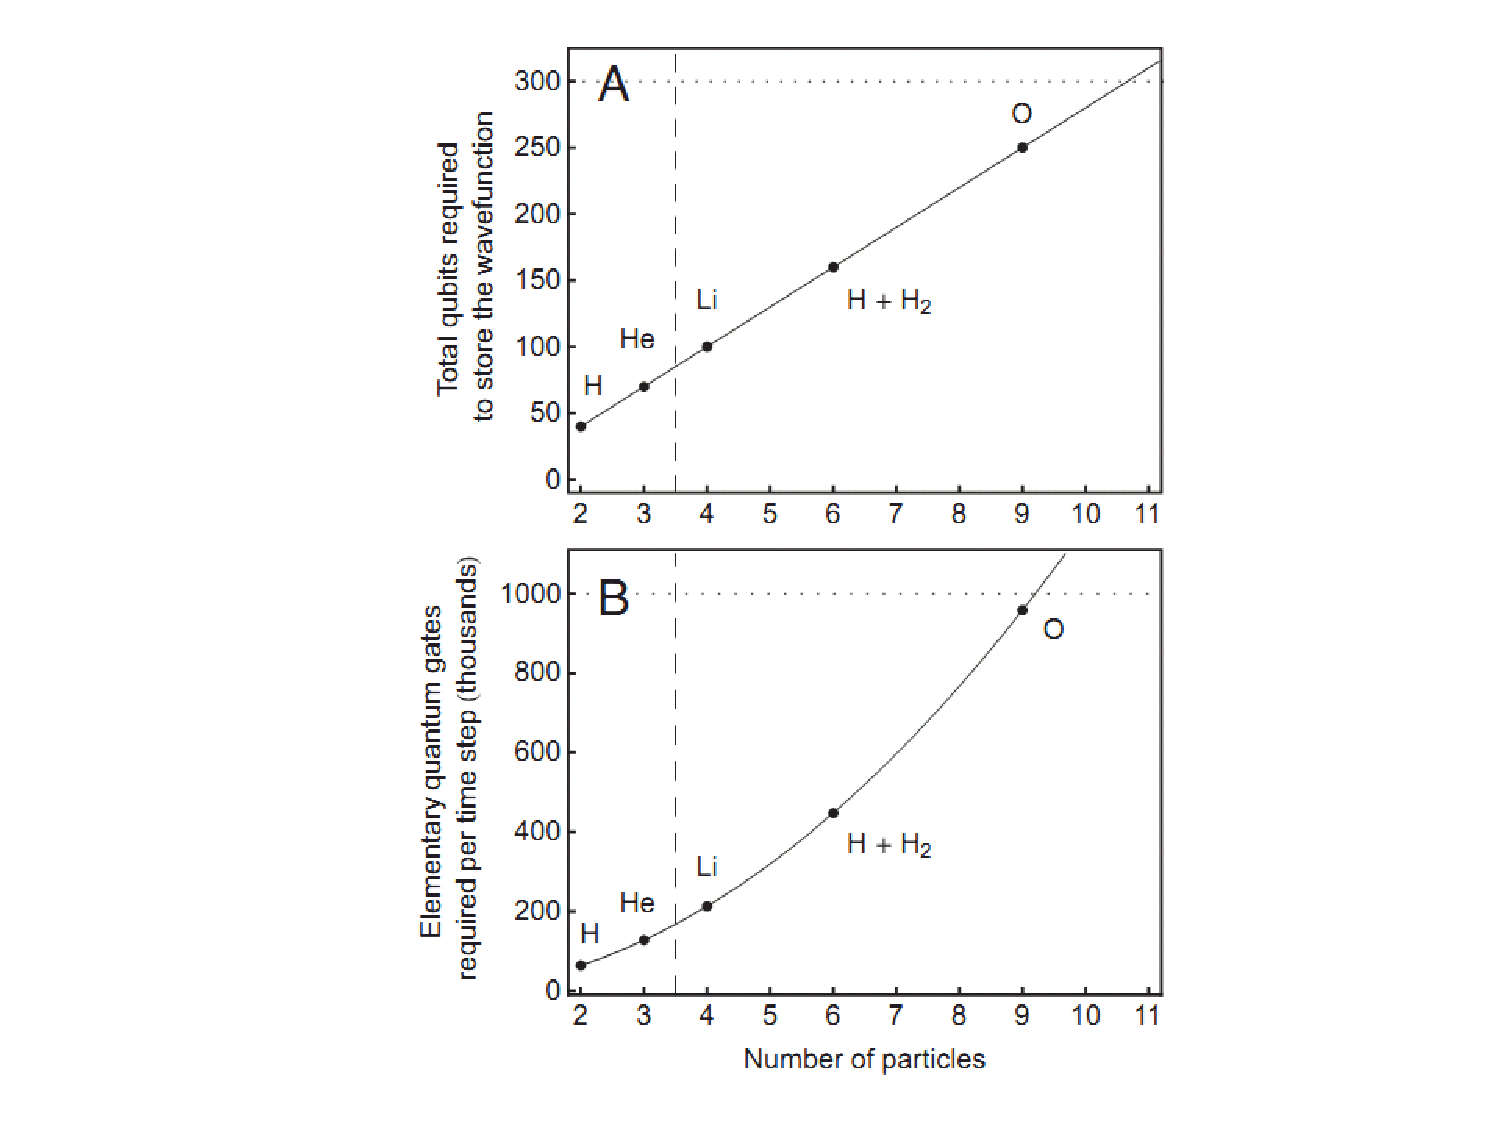
\includegraphics[width= 0.8\columnwidth]{figures/resource.pdf}
              \caption{模拟通过双势阱进行相互作用的N个粒子的资源要求。(a) 需求的比特数:对每个自由度需要$n$个qubit,每个辅助位则需要$m$个qubit,而一共需要4个辅助位,因此总共需要$n(3N-6)+4m$个qubit。水平的虚线代表一个300-qubit的
              量子计算机。(b) 需求的逻辑操作数量。一台300-qubit的量子计算机大概需要十亿个逻辑操作。取自[PNAS 105, 18681  (2008)\cite{Polynomial_time_algorithm}]。
              }
              \label{resource}
            \end{center}
        \end{figure}

\subsection{退相干和纠错}

虽然量子模拟和量子计算和环境的相互作用方式是相似的,但量子模拟中退相干并不是一个非常严重的问题,因为量子模拟需求的精度相对不高。更有趣的是,甚至有
建议模拟器的退相干还可以用来粗略调制被模拟系统的退相干\cite{Lloyd}。Tseng等也通过理论计算和实验证明\cite{deco},在开放系统的量子模拟中可以通过改变被模拟系统和模拟器之间的映射方式来
研究模拟器的退相干机制。原则上,我们可以完全分析退相干是如何影响模拟过程的,然后通过选择合理的映射方式就可以调制模拟器的有效退相干。同时利用子空间的概念
我们也可以减小退相干的影响。而且,理论和实验上也表明退相干可以对临界系统的信息获取有一定的作用\cite{deco1,deco2}。

虽然量子模拟中对精度的要求比量子算法要低,但误差还是要尽量减小的。比如为了模拟薛定谔方程我们要最小化幅度的误差\cite{schro},而对一个局域系统来说其哈密顿量以及所选择qubit的
微小改变都会指数上影响其模拟\cite{mon},而多体相互作用的哈密顿量模型中两体相互作用和局域控制操作的噪声影响也被研究过\cite{dur}。不过总体来说关于这方关于这方面的研究还是偏少。

\section{量子模拟的物理实现}

 “\emph{现代高能物理发展到了量子物理以后,有很多理论根本无法做实验,在家用纸和笔来算已经跟数学家做的差不多了。}”

 \hspace{23em} \emph{--丘成桐}

量子模拟的物理实现要求一个可控的量子系统。对DQS来说,控制的精度要求更高,AQS相对要低一些。理论上,任何可以用作量子计算机的物理系统都可以用来作量子模拟。
反过来,即使不能作为量子计算机的体系也有可能执行AQS,比如BEC中的声波传播子可以用来模拟宇宙膨胀\cite{cosmic}。 当然关于潜在的量子计算方案我们已在第一章讨论过,本节我们将主要关注量子模拟的物理实现。

\subsection{中性原子}

光晶格中的中性原子\cite{atomsim1}非常适合用作模拟凝聚态系统\cite{atomsim2,atomsim3}。自从利用光晶格中的冷原子模拟超流到Mott绝缘体的相变\cite{mott}的第一个实验以来,
中性原子体系模拟凝聚态的工作越来越多。理论和实验的综述性回顾可以分别参见参考文献\cite{atomsim2,atomsim1}。

        \begin{figure}[htbp]
            \begin{center}
              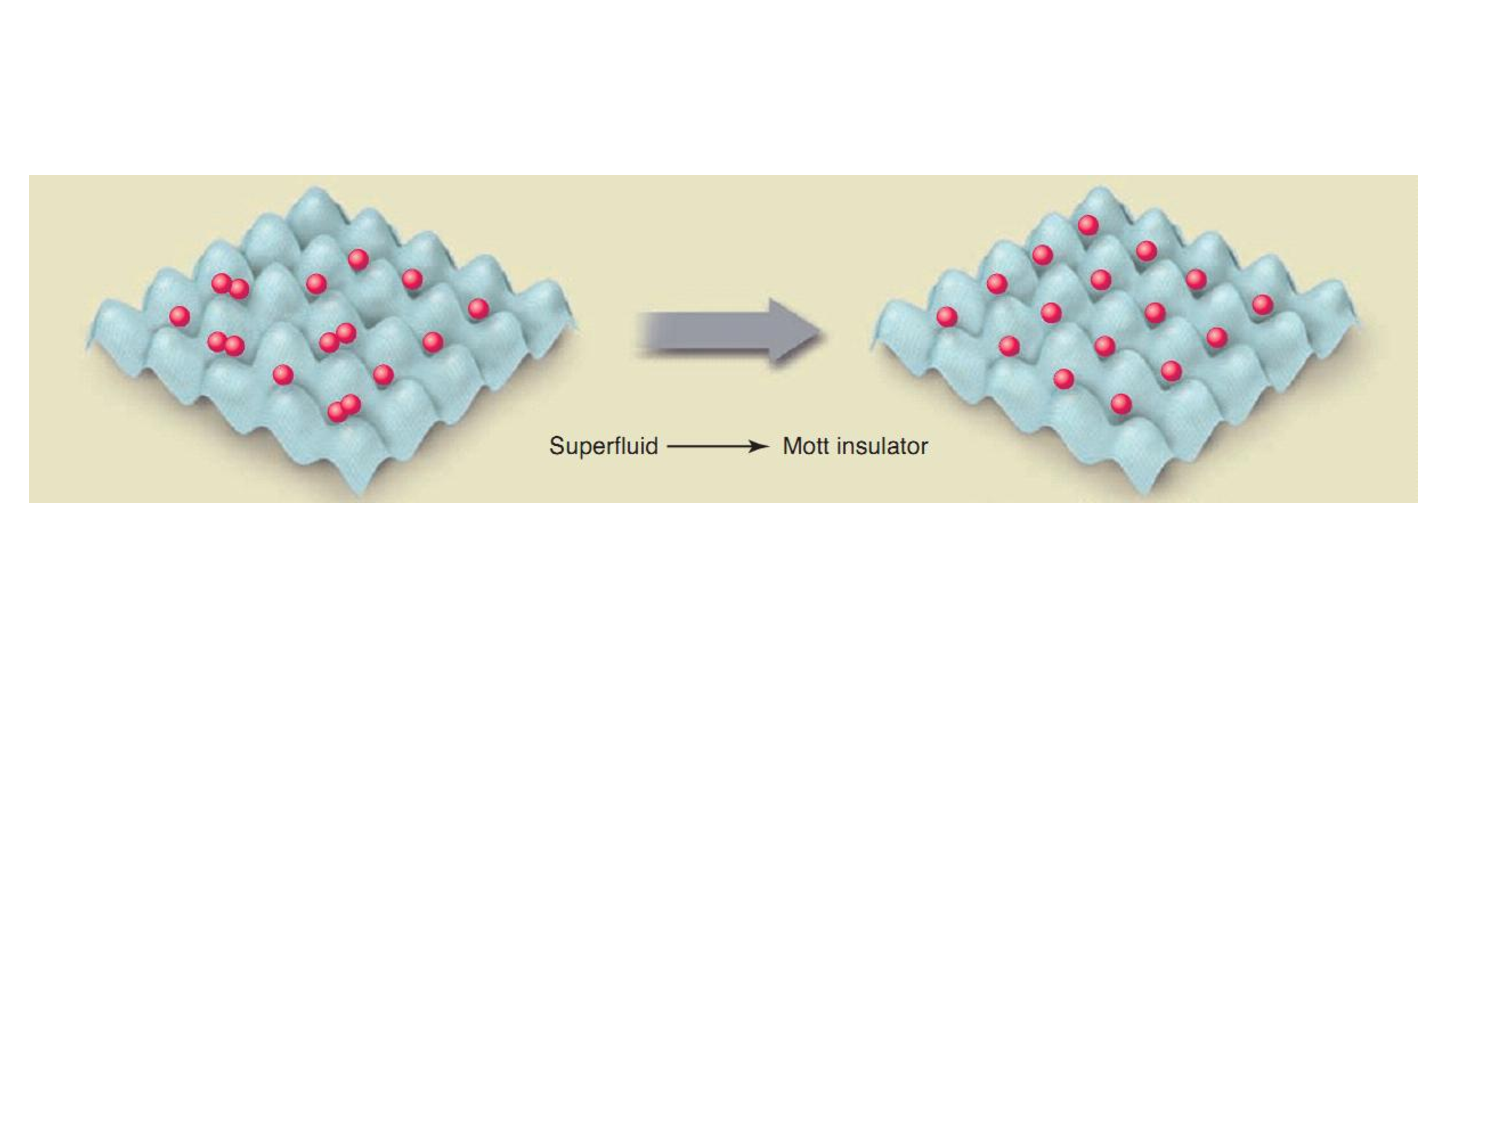
\includegraphics[width= 0.8\columnwidth]{figures/mott.pdf}
              \caption{利用中性原子模拟超流到Mott绝缘体的相变。隧穿能量和本地相互作用能量的比率依靠晶格势场深度来调节,以确保相变发生。取自[Science, 326, 108 (2009)\cite{simreview}]。
              }
              \label{mott}
            \end{center}
        \end{figure}

在中性原子体系中,可调节的参数非常多,所以该系统的使用非常灵活。这些可调节参数包括:隧穿能量,本地相互作用,近邻相互作用,长程相互作用,多粒子相互作用,外部
势场,Rabi振荡等。而光晶格中最常见的哈密顿量形式是Hubbard型\cite{atomsim2}:
 \begin{equation}\label{optical}
 H = H_{hop}+H_{int}+H_{pot}+H_{Rabi},
\end{equation}
其中$H_{hop}$是原子从一个晶格隧穿到另一个晶格的哈密顿量,$H_{int}$是相互作用项,$H_{pot}$是原子感受到的所有势场,$H_{Rabi}$则是原子的内部跃迁哈密顿量。
从这个哈密顿量形式出发很多问题都可以被模拟,包括DQS和AQS。
量子模拟主要通过改变晶格势场的深度或者通过Feshbach共振改变原子-原子间的相互作用来实现,不过光晶格中的单个qubit寻址非常困难,也导致该体系实现一些量子模拟任务时
有些不便。

目前除了模拟超流到Mott绝缘体的相变的实验外,其他的利用中性原子的量子模拟实验包括Tonks-Girardeau Gas的产生\cite{atomsim4}
,BSC-BEC交叉的观测\cite{atomsim5},无序系统的研究\cite{atomsim6,atomsim7}等等。

\subsection{极性分子}

极性分子可以用来模拟拓扑序\cite{polar1,polar2},其优势在于通过控制外加DC和AC的微波场,它的电偶极项可以产生非常强的偶极-偶极相互作用
,非常适合研究强关联系统。利用微波激发,偶极-偶极相互作用,自旋-轨道耦合等,极性分子可以模拟很多自旋模型,包括引申的Hubbard模型\cite{polar3},
量子相变\cite{polar4},或者三角晶格中的超固体(supersolid)相\cite{polar5}等等。关于利用极性分子模拟凝聚态物理的综述性文献可以参见Pupillo等在arXiv上的文章\cite{polar6}。 \begin{figure}[htbp]
            \begin{center}
              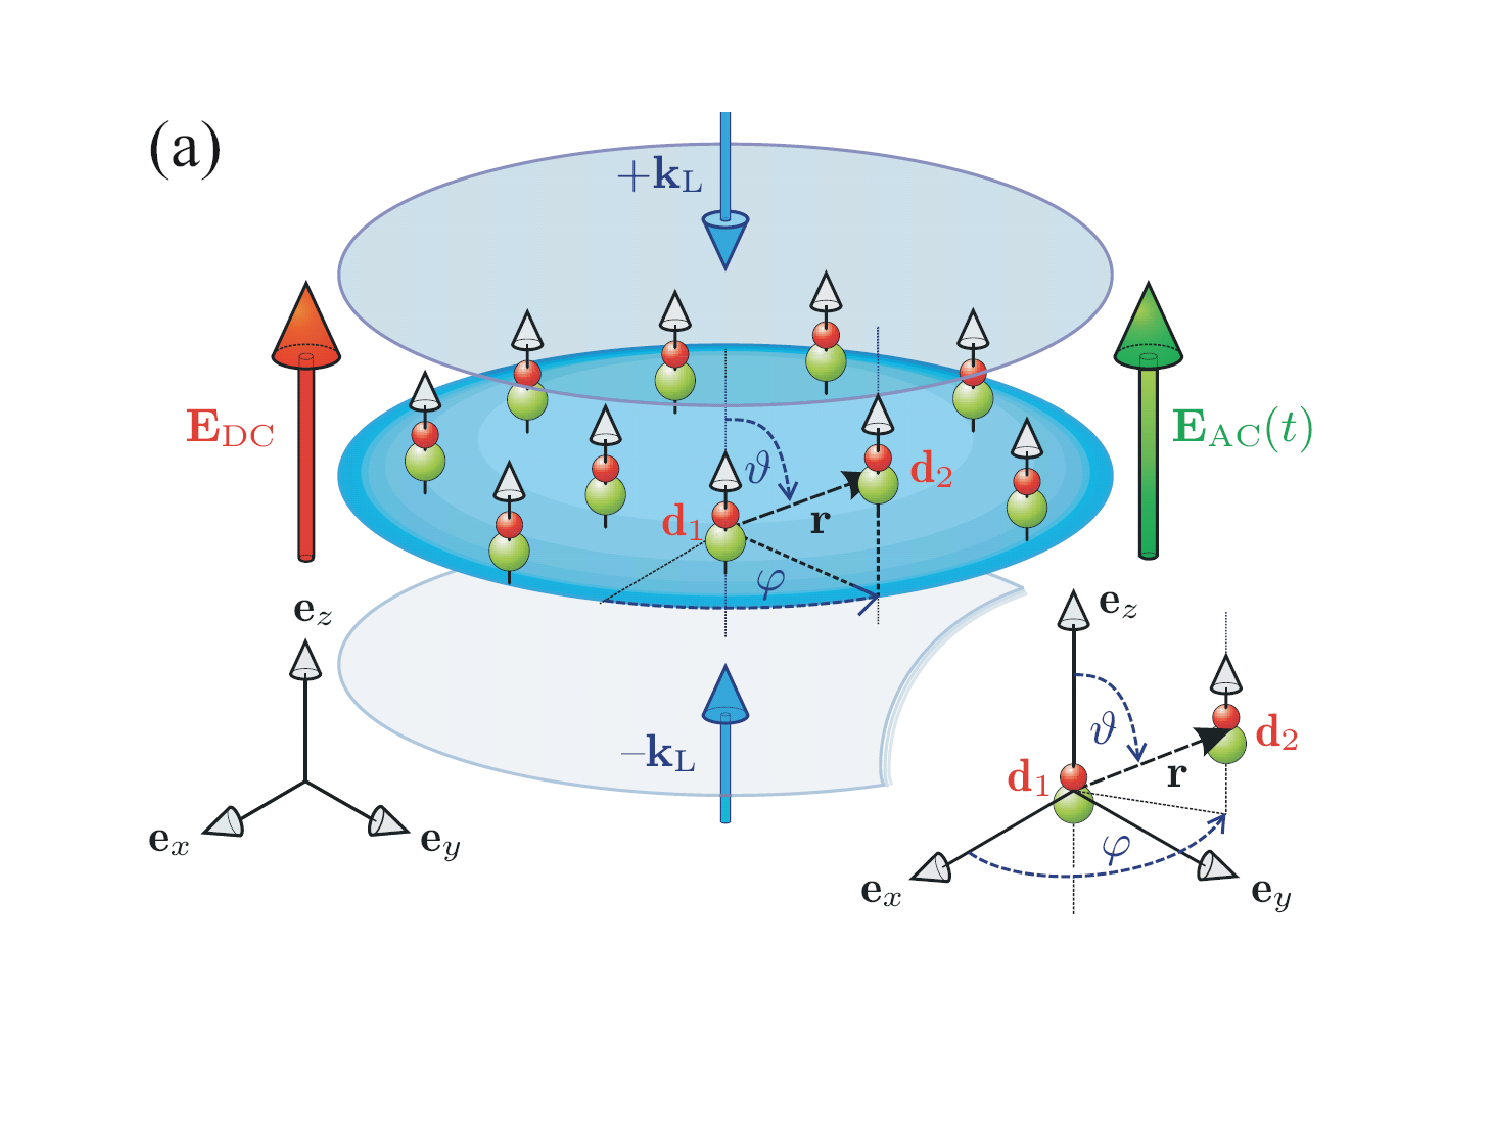
\includegraphics[width= 0.8\columnwidth]{figures/polar.pdf}
              \caption{利用反向传播的激光束可以产生光晶格中的极性分子。蓝色箭头为激光波矢,红色和绿色箭头分别为DC和AC微波场。取自[arXiv:0805.1896 (2008)\cite{polar6}]。
              }
              \label{polar}
            \end{center}
        \end{figure}

\subsection{离子阱}

离子阱体系的哈密顿量形式中可控参数也比较多,因此也可以用作DQS和AQS。利用激光激发将内部能级和振动模式耦合起来的哈密顿量形式为
 \begin{equation}\label{ion}
 H = i\hbar \eta \Omega [e^{i\phi}\sigma_{+}a-e^{-i\phi}\sigma_{-}a^{\dagger}],
\end{equation}
其中$\Omega$是Rabi跃迁频率,$\sigma_{+}$和$\sigma_{-}$是两能级的升降算子,$\eta$是Lamb-Dicke参数,$a^{\dagger}$和$a$是振动模式中
的产生和湮灭算子,$\phi$是激光相位。从这个形式中可以看出单比特门,两比特门甚至三比特门(例如Toffoli)都可以实现。

离子阱中的第一个量子模拟方案可以追溯到1998年\cite{ionsim1},第一个实验则是2002年的非线性干涉仪的模拟\cite{ionsim2}。此外,离子阱还可以用来模拟顺磁性到铁磁
性的相变\cite{ionphase},自旋1/2系统中的对相互作用\cite{ionsim3},相互作用玻色子模型\cite{ionsim4},开放系统\cite{ionsim5},Dirac粒子\cite{dirac},甚至宇宙膨胀中的Unruh效应\cite{unruh}等。

\begin{figure}[htbp]
            \begin{center}
              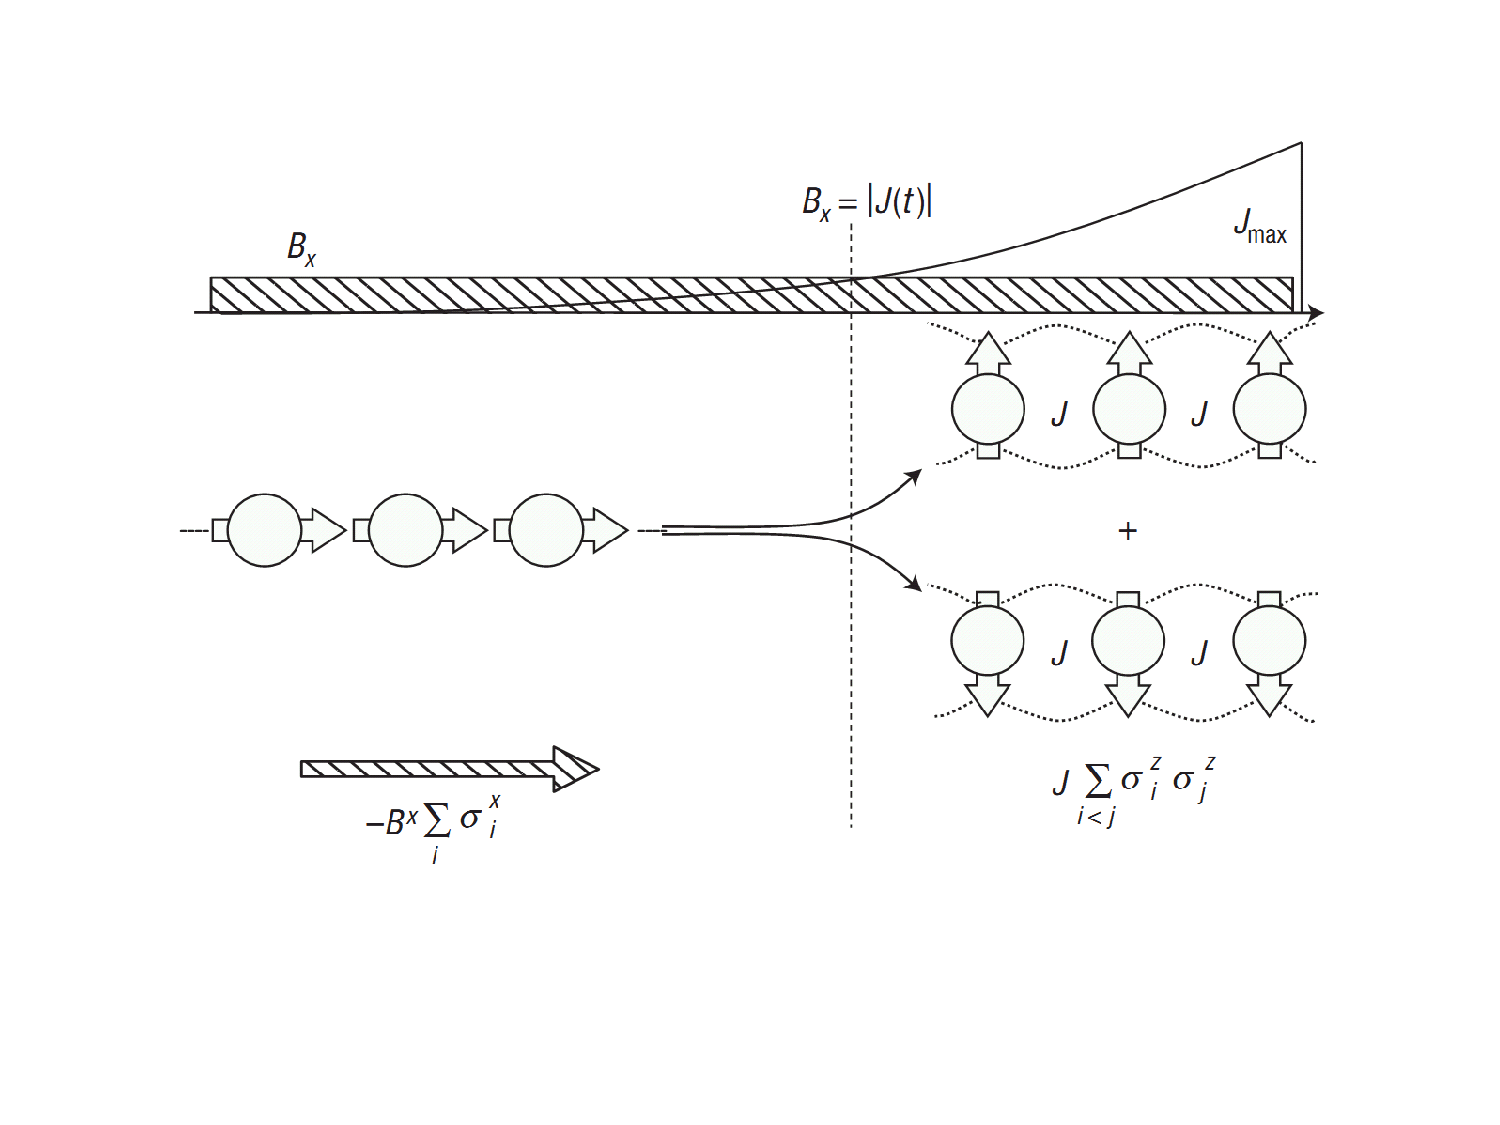
\includegraphics[width= 0.8\columnwidth]{figures/ionsim.pdf}
              \caption{利用离子阱模拟磁性的量子相变。单个自旋依靠射频场把内部能级耦合起来模拟,而自旋-自旋相互作用通过态依赖的光偶极力产生。取自[Nature Phys. 4, 757 (2008)\cite{ionphase}]。
              }
              \label{ionsim}
            \end{center}
        \end{figure}

\subsection{核磁共振}

用核磁共振手段操控的核自旋是最早在实验上执行量子模拟的体系之一。NMR中哈密顿量的形式一般是
 \begin{equation}\label{ion}
 H = -\hbar \gamma I\cdot B+\sum_{i>j}J_{ij} I_i \cdot I_j,
\end{equation}
其中$\gamma$是旋磁比,$I$是角动量算符,$B$是外加磁场,$J_{ij}$是自旋-自旋之间的耦合相互作用。NMR中的技术非常成熟,但它主要的缺点在于可扩展性。
虽然固体NMR在某种意义上可以克服这个问题,但在高维情况下。单比特的寻址以及测量依然非常困难。不过尽管如此,NMR依然非常适合作为小体系量子模拟任务的测试平台,
包括DQS和AQS。

最早的NMR量子模拟实验是利用核自旋模拟谐振子和非谐振子的动力学行为\cite{nmrsim1}。其他的一些实验包括模拟三体相互作用\cite{nmrsim2,app15},开放系统\cite{nmrsim3},量子混沌\cite{chaos2},Fano-Anderson哈密顿量\cite{nmrsim4},
量子相变\cite{nmrsim5,nmrsimphase,app16},哈密顿量对模型\cite{nmrsim6},量子化学等等\cite{static,dynamical,yexiao}。
\begin{figure}[htbp]
            \begin{center}
              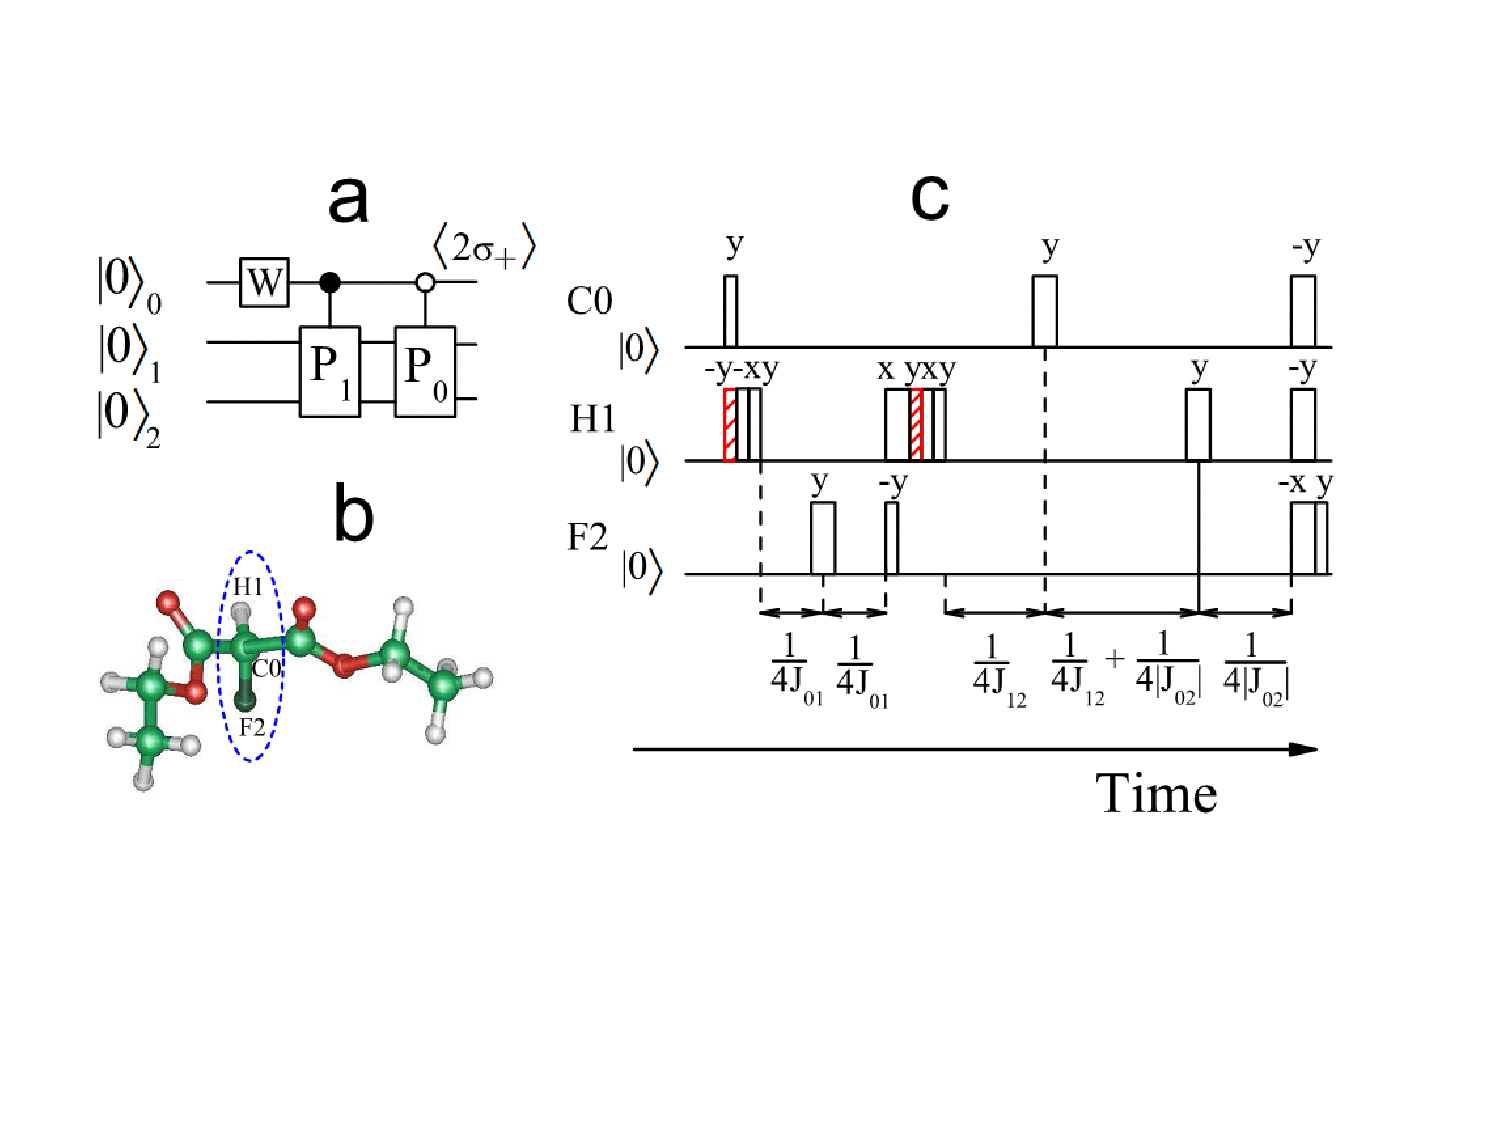
\includegraphics[width= 0.8\columnwidth]{figures/nmrsim.pdf}
              \caption{(a) 利用一个探测qubit测量量子相变的网络图。W是Walsh-Hadamard变换。(b) NMR实验所用的3-qubit样品Diethyl-fluoromalonate。(c) 测量量子态交叠度的脉冲序列图。取自[Phys. Rev. Lett. 100, 100501 (2008)\cite{nmrsimphase}]。
              }
              \label{nmrsim}
            \end{center}
        \end{figure}

\subsection{光子}

由于光子体系的操控灵活性非常低,而且可扩展性也非常有限,所以利用光学体系的量子模拟实验非常少。比较有代表性的工作有
量子混沌\cite{chaos1},任意子的分数统计\cite{anyons1},以及氢分子基态能级模拟的实验\cite{optics_static}。
\begin{figure}[htbp]
            \begin{center}
              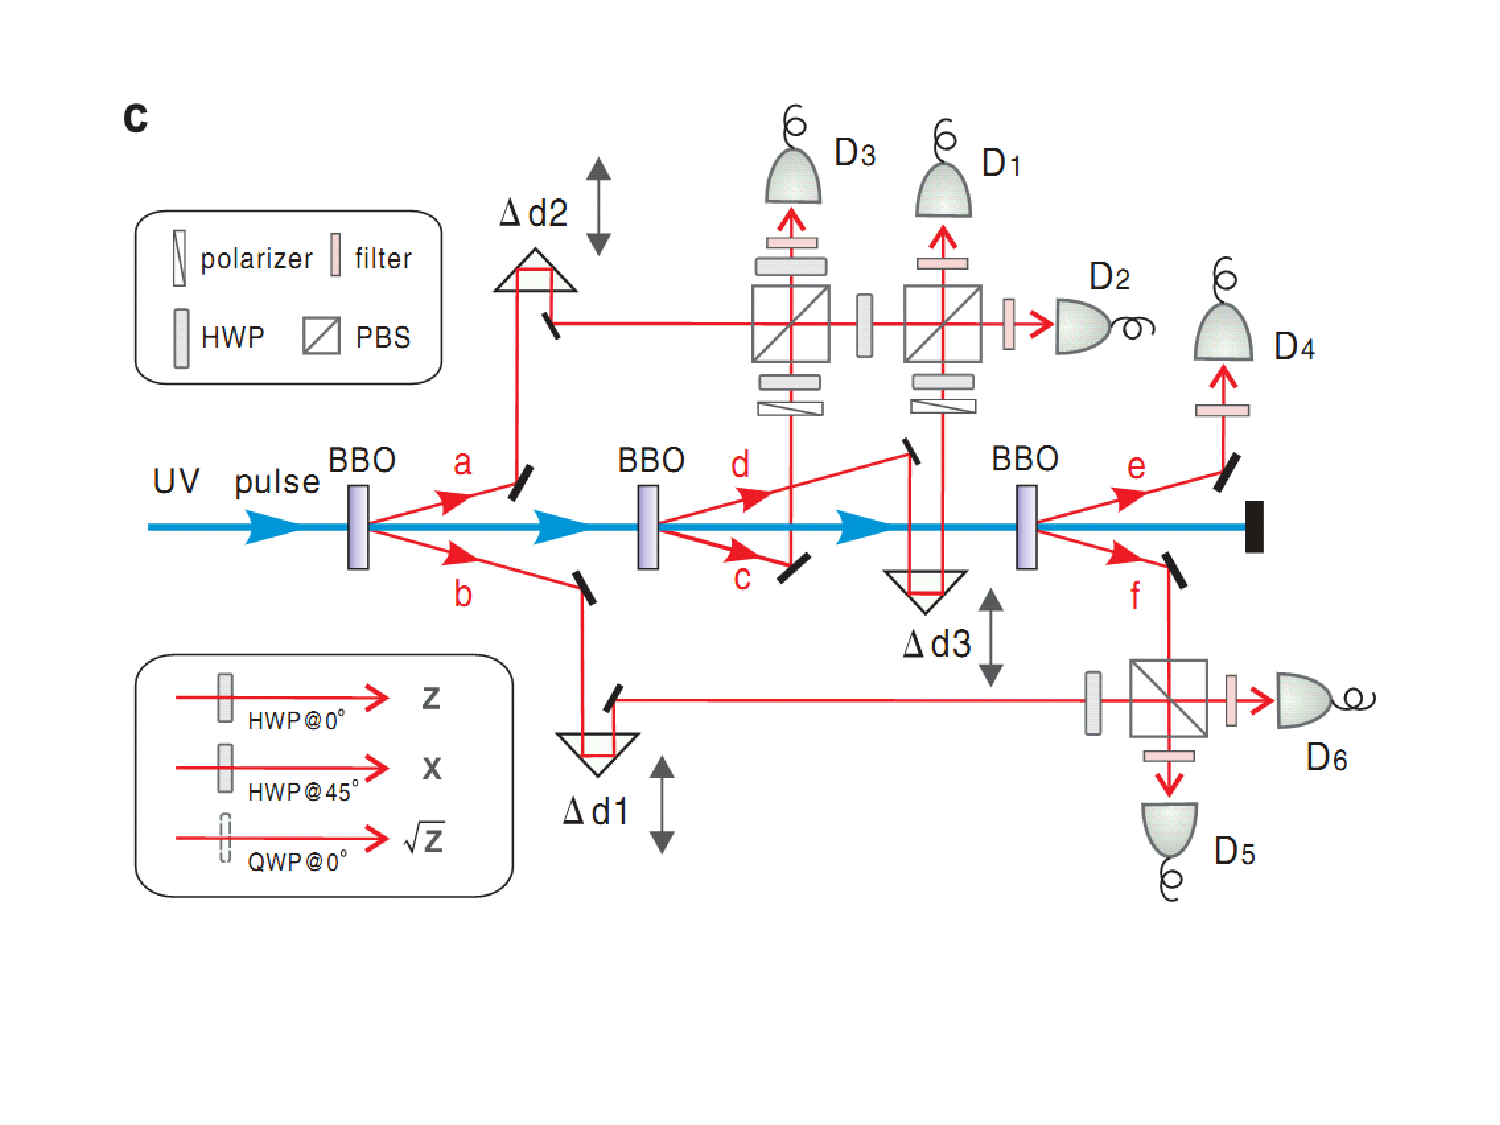
\includegraphics[width= 0.8\columnwidth]{figures/photons.pdf}
              \caption{测量任意子分数统计的实验装置。一束紫外激光通过三个BBO后可以产生三对纠缠的光子。取自[Phys. Rev. Lett. 102, 030502 (2009)\cite{anyons1}]。}
              \label{photons}
            \end{center}
        \end{figure}

\subsection{量子点}

半导体量子点中的电子自旋\cite{dotsim1}也是可以用来作量子模拟的。由于量子点是半导体器件,其激发被限制在一维或二维的很小的区域上。一旦该区域的大小和电荷载体的波长大致
相等,就有了分离的能级结构,此时量子点的行为就非常类似于一个真正的原子。同时,量子点的操控也比较灵活,而且技术上用光激发也比较容易,因此是非常合适的
实验量子模拟体系。量子点的哈密顿量一般形式为
 \begin{equation}\label{dotsim}
 H = \sum_{j=1}^n\mu_B g_j(t) B_j(t)\cdot S_j +\sum_{1\leq j<k\leq n} J_{jk}(t)S_j\cdot S_k,
\end{equation}
其中第一个求和项是外加磁场引起的能量,第二个求和项是加在量子点之间的栅电压产生的隧穿效应引起的相互作用哈密顿量。相对于囚禁在光晶格中的原子,
量子点的接近Fermi温度的极低温要求可以实现自然的长程Coulomb相互作用\cite{dotsim2}。

量子点中可以执行的量子模拟任务有Fermi-Hubbard模型\cite{dotsim2},高温超导体中的CuO平面\cite{dotsim3},甚至化学反应\cite{reaction}等等。 \begin{figure}[htbp]
            \begin{center}
              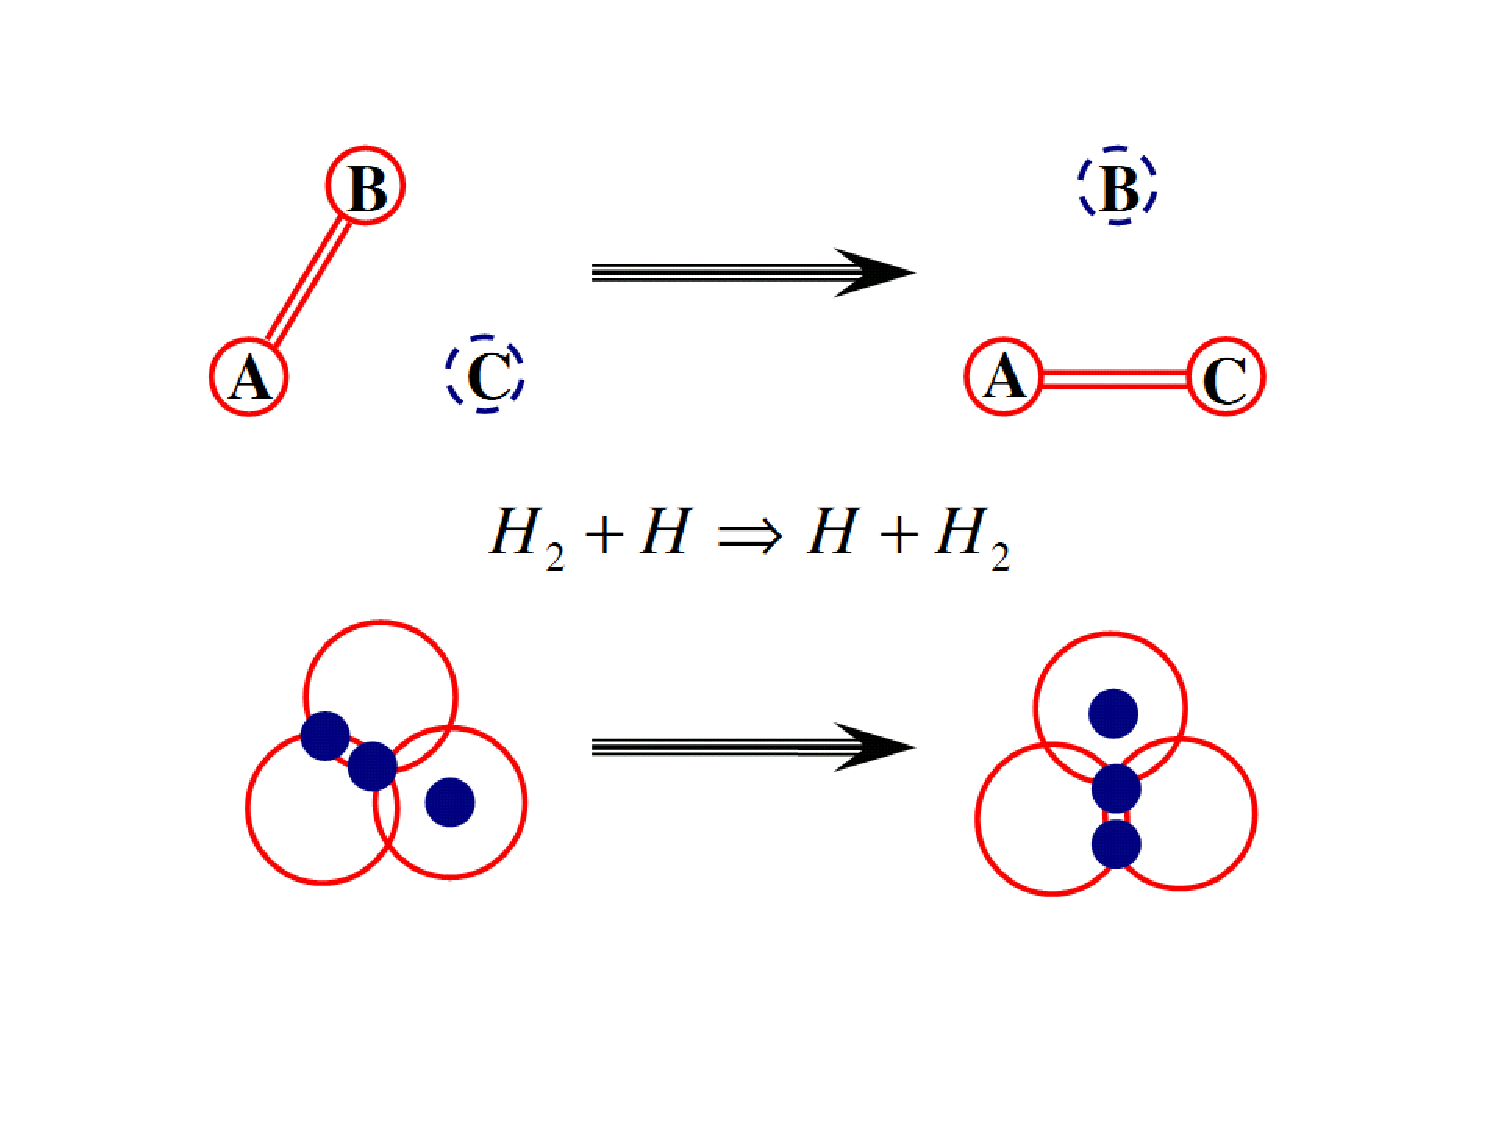
\includegraphics[width= 0.8\columnwidth]{figures/dotsim.pdf}
              \caption{H$_2$+H$\longrightarrow$H+H$_2$化学反应的示意图(上半部分)以及耦合量子点系统中
              电子的重新分配(下半部分)。取自[Euro. Phys. Lett. 80, 67008 (2007)\cite{reaction}]。
              }
              \label{dotsim}
            \end{center}
        \end{figure}

\subsection{超导线路}

虽然超导线路是肉眼可见的,但它表现出了很强的量子行为,因此可以被理解为“模拟原子”。和真正的原子比起来,超导线路中的特征频率和一些其他参数都可以被
精心设计和构造,比如共振频率可以通过外加参数调制,耦合强度则可以依据实验要求随时开关。通过电容(电感)耦合起来的电荷(磁通)qubit的哈密顿量可以写成
 \begin{equation}\label{supersim}
 H = -\sum_{i=1}^N \frac{\Delta_i}{2} \sigma_i^z-\sum_{i,j}J_{ij} \sigma_i^x\sigma_j^x,
\end{equation}
其中$\Delta_i>0$是能级劈裂,$J_{ij}$是耦合强度。超导线路中的单个比特控制和测量都已经解决的很好,但可扩展性问题依然有待解决。

除了最早的观测通过量子涡流形成的一维Mott绝缘体\cite{supersim1}的工作外,超导线路还可以用来模拟原子物理和量子光学中\cite{supersim5}的许多现象,蜂巢状晶格上的Kitaev模型\cite{supersim2},Anderson和Kondo模型\cite{supersim3},
可调材料\cite{supersim4}等等。

\begin{figure}[htbp]
            \begin{center}
              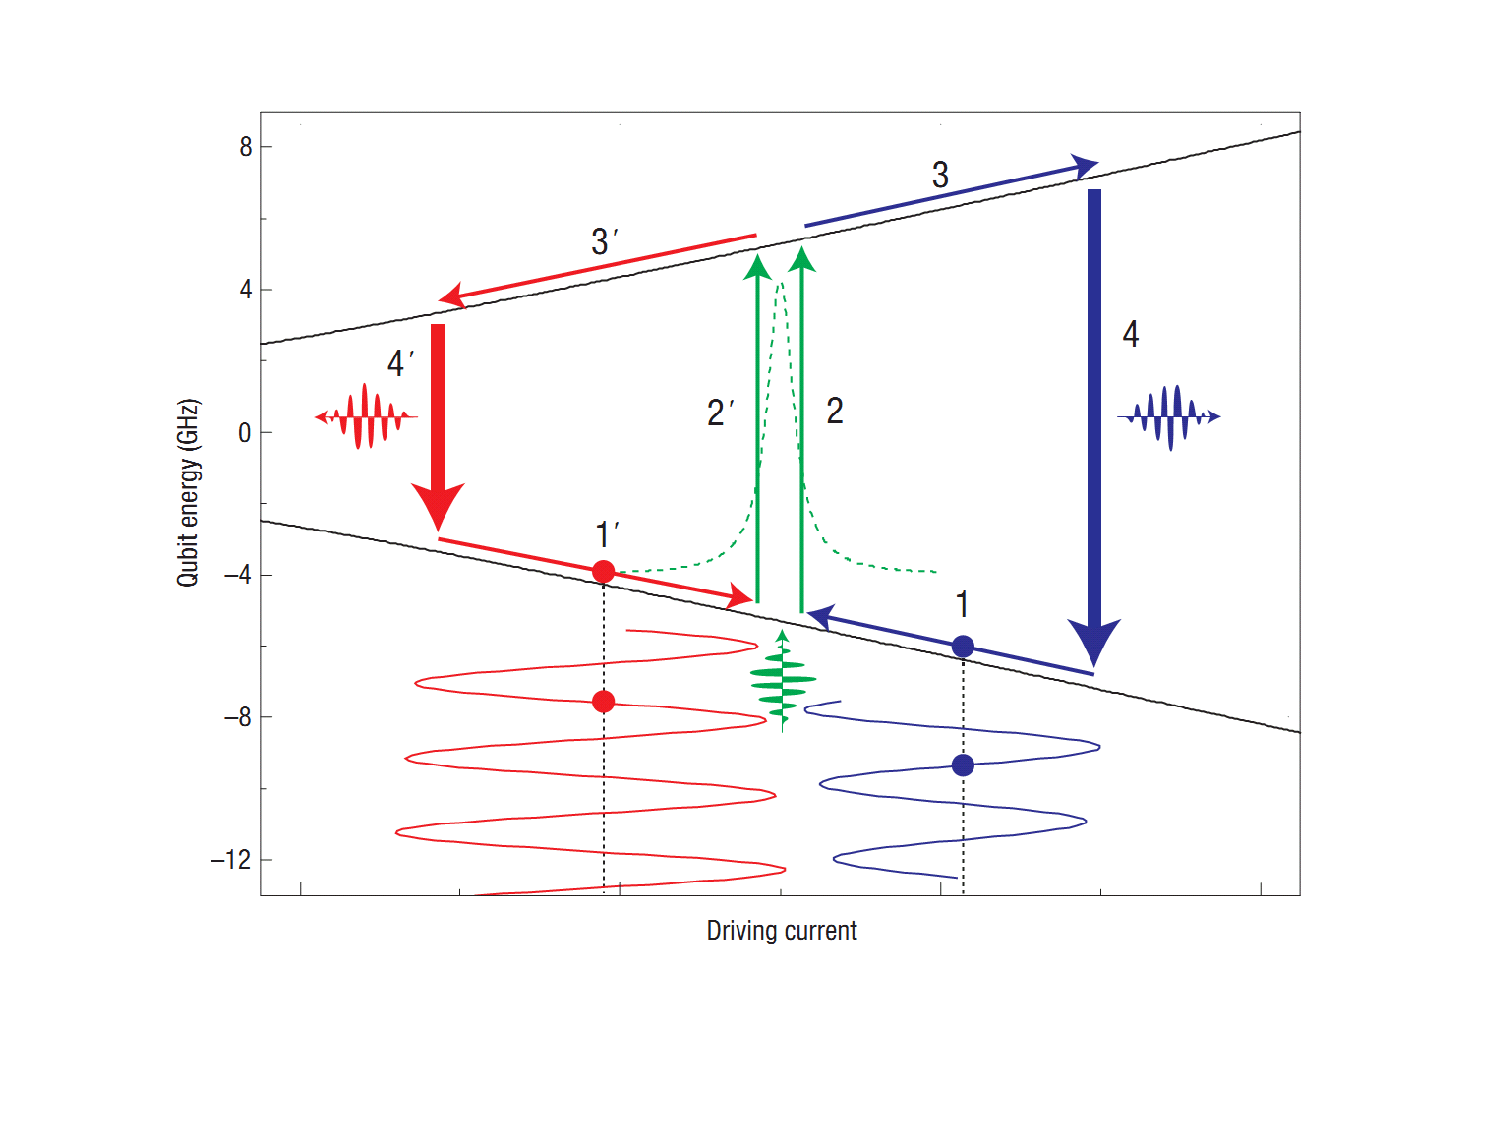
\includegraphics[width= 0.8\columnwidth]{figures/supersim.pdf}
              \caption{利用介观线路模拟Sisyphus(希腊神话中的科林斯王)冷却。$1\longrightarrow2\longrightarrow3\longrightarrow4$的循环
              模拟了原子物理中的Sisyphus冷却,以及希腊神话中科林斯王的命运。取自[Nature Phys. 4, 589 (2008)\cite{supersim5}]。
              }
              \label{supersim}
            \end{center}
\end{figure}

 \section{量子模拟的应用}

  “\emph{每引入一个方程式,就会使读者减少一倍。}”

 \hspace{23em} \emph{--史蒂芬·霍金}

从前面对量子模拟领域的介绍来看,量子模拟至少在物理和化学上肯定有很广泛的应用。不仅如此,它在生物和材料学,甚至宇宙学上也能解决一些经典计算上难以
处理的问题。特别的,如果是模拟量子系统,量子模拟器更是可以预言一些新结论,测试一些新模型,而这些都是经典模拟方法做不到的。本节我们就将介绍
到底有哪些困难的问题可以用量子模拟解决。

 \subsection{凝聚态物理}

 凝聚态物理中存在非常多种经典上难以处理的多体问题,下面我们将具体讨论这些问题。

 \emph{1. Hubbard模型}

 对于存在于一个晶格上的相互作用的粒子来说,Hubbard模型是最简单的模型。但是,在大量粒子及高维的情况时,这个问题就很难在经典上处理了。
 通过DQS我们可以有效模拟Hubbard模型。针对如何获得费米Hubbard哈密顿量的能级谱
 \begin{eqnarray}\label{supersim}
 H_H &=& -\sum_{(i,j);\sigma}[t_x(a^{\dagger}_{(i,j);\sigma}a_{(i+1,j);\sigma}+a^{\dagger}_{(i+1,j);\sigma}a_{(i,j);\sigma})+t_y(a^{\dagger}_{(i,j);\sigma}a_{(i,j+1);\sigma}+a^{\dagger}_{(i,j+1);\sigma}a_{(i,j);\sigma})]\nonumber \\
 &&+U\sum_{(i,j)}n_{(i,j);\uparrow} n_{(i,j);\downarrow},
\end{eqnarray}
Somma等详细讨论了该模型与DQS之间的映射,以及初态制备,演化,测量等所有步骤\cite{mea1}。同时,该模型在Ho等人的工作中也有讨论\cite{hubbard1}。

当然,该模型也可以用AQS的思想来研究,比如在量子点中\cite{dotsim2},极性分子中\cite{polar3}以及离子阱\cite{ionsim4}中都有涉及Hubbard模型。

 \emph{2. 量子相变}

 当一个物理参量在绝对零度下发生改变时,量子相变就可能发生,它描述的是一个多体系统中因为量子涨落导致的基态能级突变。量子相变是非常基础但非常重要的领域之一,
 可惜在经典上模拟或者实验都非常困难,而对量子相变的深入研究会提高我们对纯净量子现象的认识。量子模拟实验第一个观测到的相变是利用光晶格中的中性原子模拟从超流到Mott绝缘体的相变\cite{mott},
 前面已经有了详细介绍,这里不再赘述。

 另外一种相变的粒子是量子磁性的相变,比如离子阱中利用绝热手段模拟的量子顺磁性到反铁磁性的相变\cite{ionphase},该工作利用离子阱平台重复了我们在NMR系统中的量子相变模拟工作\cite{nmrsim5}。该系统可以用简单的Ising模型描述
 \begin{equation}\label{supersim}
 H_I = -B_x\sum_i \sigma_i^x+\sum_{i<j}J_{ij}\sigma_i^z\sigma_j^z,
\end{equation}
其中$B_x$是磁场强度,$J_{ij}$是自旋-自旋相互作用。通过绝热改变相互作用强度,同时保持外磁场$B_x$为常数,我们可以观测到系统从一个顺磁性状态
$\left\vert \rightarrow \right\rangle \left\vert \rightarrow \right\rangle$变到一个反铁磁性状态$\left\vert \uparrow \right\rangle \left\vert\uparrow \right\rangle+\left\vert \downarrow \right\rangle \left\vert\downarrow \right\rangle$。

  \emph{3. 自旋模型}

 考虑最简单的Heisenberg自旋哈密顿量模型
  \begin{equation}\label{supersim}
 H_{XYZ} = \sum_{i=1}^N[J_x\sigma_i^x\sigma_{i+1}^x+J_y\sigma_i^y\sigma_{i+1}^y+J_z\sigma_i^z\sigma_{i+1}^z].
\end{equation}
在离子阱中,XY以及XYZ模型相互作用都已通过利用集体振动模式实现\cite{model1},自旋链和自旋梯的模型也已在光晶格中被讨论\cite{model2};高维或者不规则维度
的自旋模型则被认为可以在超导线路中模拟\cite{model3};反铁磁的Heisenberg模型则可以通过固态NMR实现\cite{model4}。

\begin{figure}[htbp]
            \begin{center}
              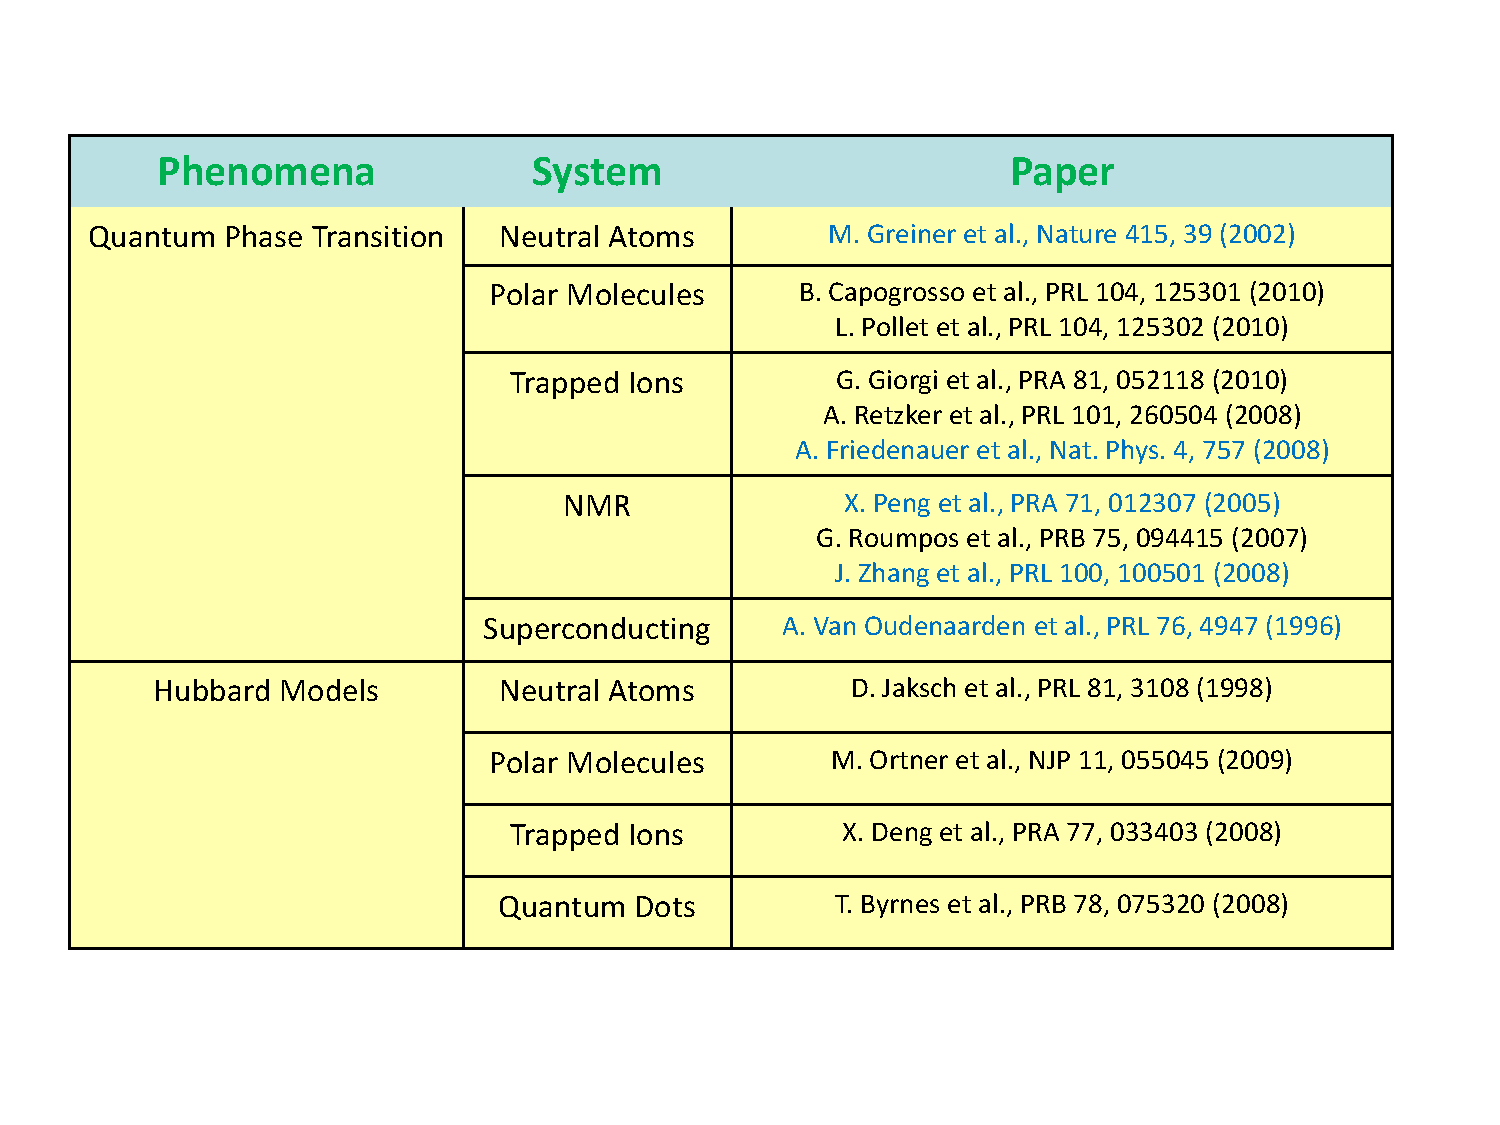
\includegraphics[width= 0.8\columnwidth]{figures/simcondense1.pdf}
              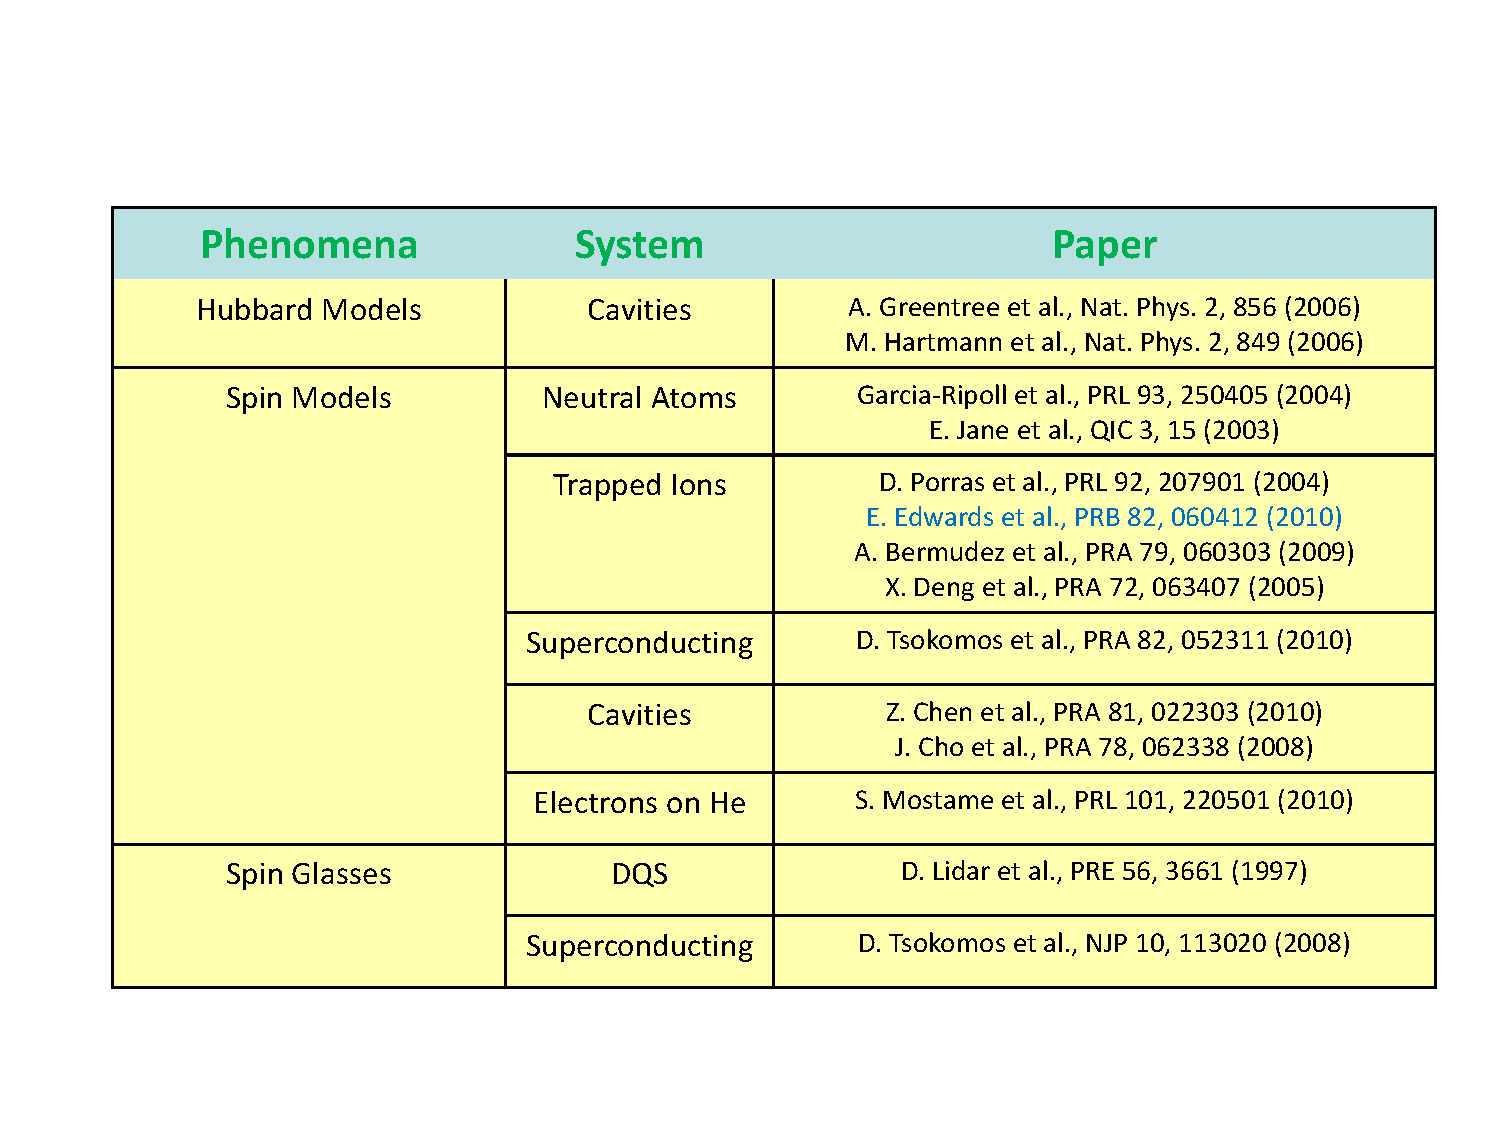
\includegraphics[width= 0.8\columnwidth]{figures/simcondense2.pdf}
              \caption{量子模拟在凝聚态物理中的应用(上)。蓝色字体为实验进展,黑色字体为理论进展。
              }
              \label{supersim}
            \end{center}
\end{figure}


\emph{4. 无序系统}

无序系统在凝聚态中的很多困难问题中出现,比如输运,传导,自旋玻璃,高温超导等等。而经典上关于无序系统的处理非常具有挑战性,因此有很多的量子模拟算法
被提出来。例如,Fano-Anderson模型的哈密顿量为
 \begin{equation}\label{supersim}
 H_{FA} = \sum_{l=1}^{n-1}\varepsilon_{k_l} c^{\dagger}_{k_l} c_{k_l}+\epsilon b^{\dagger}b+V(c^{\dagger}_{k_0}b+c_{k_0}b^{\dagger}),
\end{equation}
其中费米算符$c^{\dagger}_{k_l}(c_{k_l})$和$b^{\dagger}(b)$分别可以在导电模式和杂质中产生(湮灭)非自旋费米子。该模型已经在NMR上实验实现\cite{nmrsim4}。

而在AQS的方案中,光晶格可以实验实现无序系统且观测到Bose-glass相\cite{atomsim7};无序势阱中可以研究BEC的Anderson-like局域化\cite{atomsim6};
离子阱可以用来研究无序系统中的物理现象\cite{dis1};描述导电区的磁性杂质的哈密顿量则可以映射到超导线路\cite{supersim3}。

\emph{5. 高温超导}

包含氧化铜的复合物中的高温超导也是一个可以用量子模拟解决的难题。利用量子点我们可以用AQS的方式模拟高温超导体\cite{dotsim3},$t-J$模型也被证明可以被模拟\cite{high1}.
BCS对模型的哈密顿量则可以用DQS来模拟,其一般形式为
 \begin{equation}\label{supersim}
 H_{BCS} = \sum_{m=1}^{N} \frac{\epsilon}{2}(n_m^F+n_{-m}^N)+\sum_{m,l=1}^{N}V_{ml}^{+}c_m^{\dagger}c_{-m}^{\dagger}c_{-l}c_l,
\end{equation}
$c_m^{\dagger}(c_m)$和$b_m^{\dagger}(b_m)$分别为费米和玻色的产生(湮灭)算子,$|m|=1,2,\cdots,N$为量子数。实现该模型的量子模
拟算法\cite{high2}和NMR实验\cite{nmrsim6}目前也已完成。

\emph{6. 自旋玻璃}

如果自旋间的相互作用是铁磁或反铁磁的,即使在低温下空间内的自旋取向也不再是唯一的,而会呈现出一定的随机性,这种自旋玻璃的性质也可以用DQS模拟,
比如构造Ising模型中的Gibbs分布\cite{glass1}。该算法适用于任何维度的自旋玻璃Ising模型,或者含外磁场的模型。

用AQS的方法模拟Lipkin-Meshkov-Glick模型
 \begin{equation}\label{supersim}
 H_{LMG} = -\frac{\Delta}{2}\sum_{i=1}^{N} \sigma_i^z-\frac{J}{2}(\sum_{i=1}^{N}\sigma_i^x)^2+\frac{NJ}{2},
\end{equation}
以及复杂量子系统,比如Sherrington-Kirkpatrick自旋玻璃被Tsomokos等人给出\cite{glass2},而这个模型可以在超导线路中被自然模拟。

\emph{7. 超颖材料}

量子范畴的可控超颖材料的行为也可以被量子系统模拟\cite{meta1,supersim4}。量子超颖材料的一个例子是共振腔中全同qubit的无限链模型,这种系统中有可能实现
新的控制电磁场演化的方法,而这在经典材料里是完全做不到的。

\emph{8. 拓扑序}

任意子是量子统计性质既不满足玻色性也不满足费米性的二维粒子,可以用来描述石墨烯或量子霍尔效应等现象。而且,任意子可以被用作拓扑量子计算\cite{topo1}。
该模型既可以通过小尺度的DQS模拟\cite{topo2},也可以利用中性原子用AQS的方式模拟。前者在Lu等人的文章中已经用线性光学体系实验证实\cite{anyons1},其哈密顿量为
\begin{equation}\label{supersim}
 H_{K} = -\sum_vA_v-\sum_pB_p,
\end{equation}
其中$A_v=\prod_{i\in v}\sigma_i^x$和$B_p=\prod_{i\in p}\sigma_i^z$,$v$取遍所有顶点而$p$取遍所有平面。在光晶格中满足阿贝尔和非阿贝尔性质的任意子也可以通过
增加辅助粒子来实现,利用超导线路甚至可以构筑Kitaev蜂巢模型\cite{anyons2}。不仅对量子模拟,这些方案对拓扑量子计算的发展也有很大贡献。


\begin{figure}[htbp]
            \begin{center}
              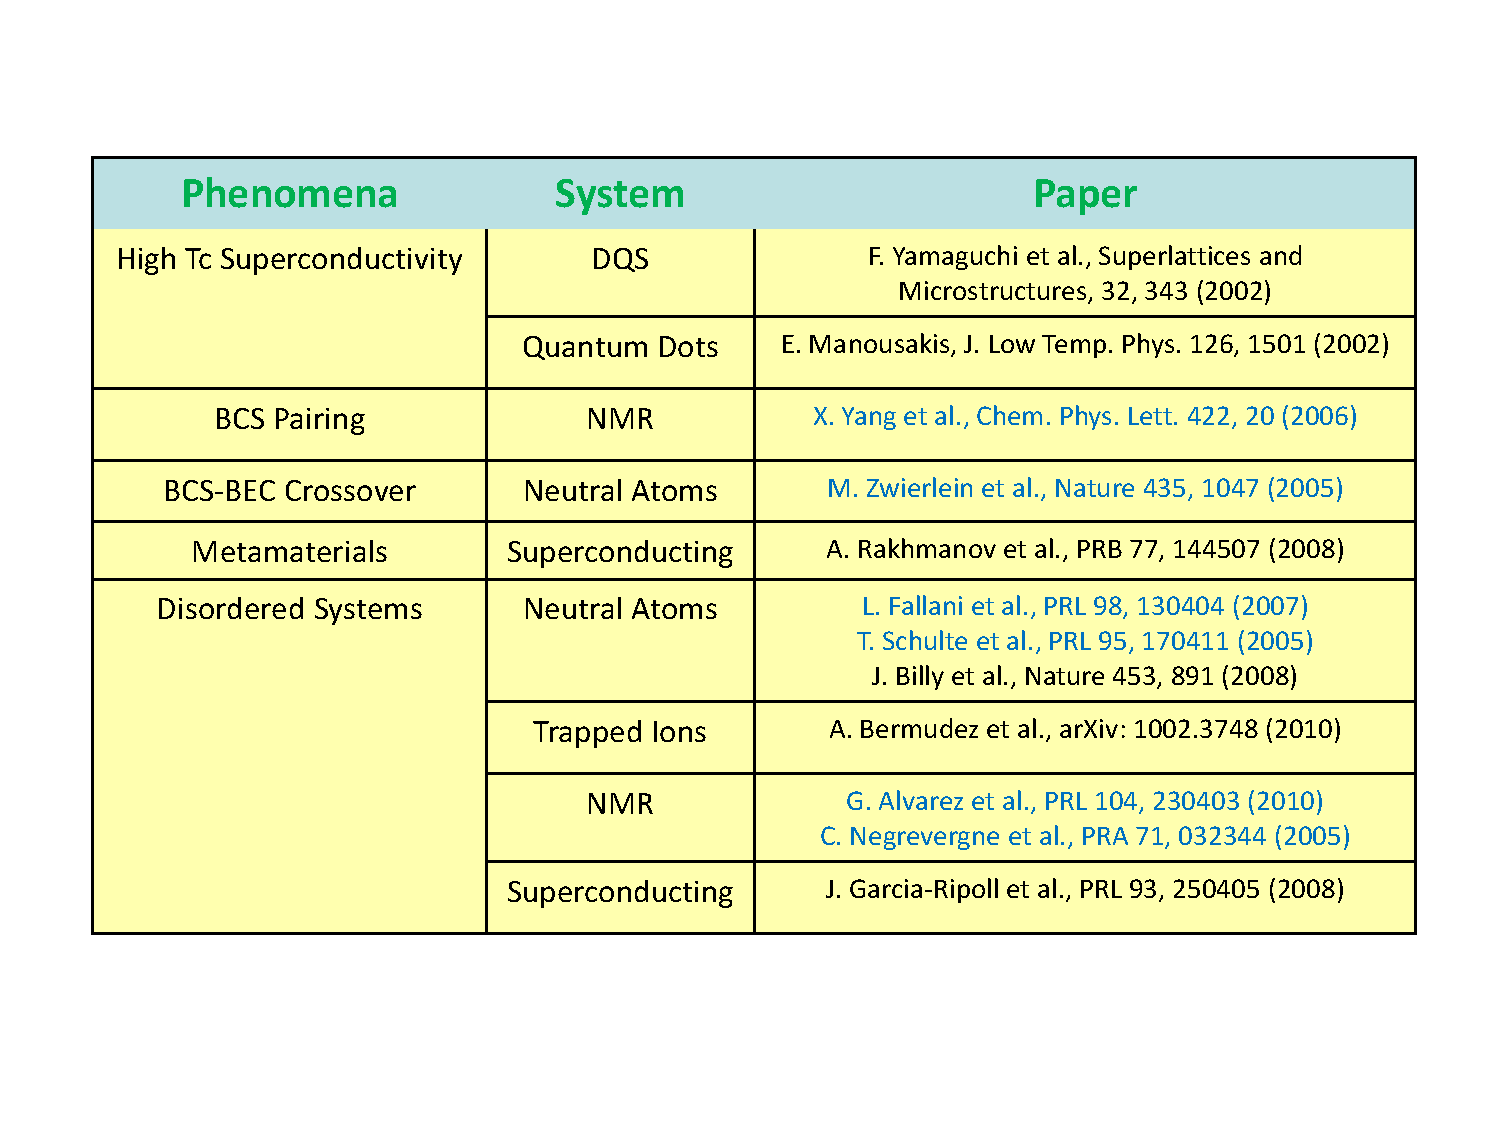
\includegraphics[width= 0.8\columnwidth]{figures/simcondense3.pdf}
              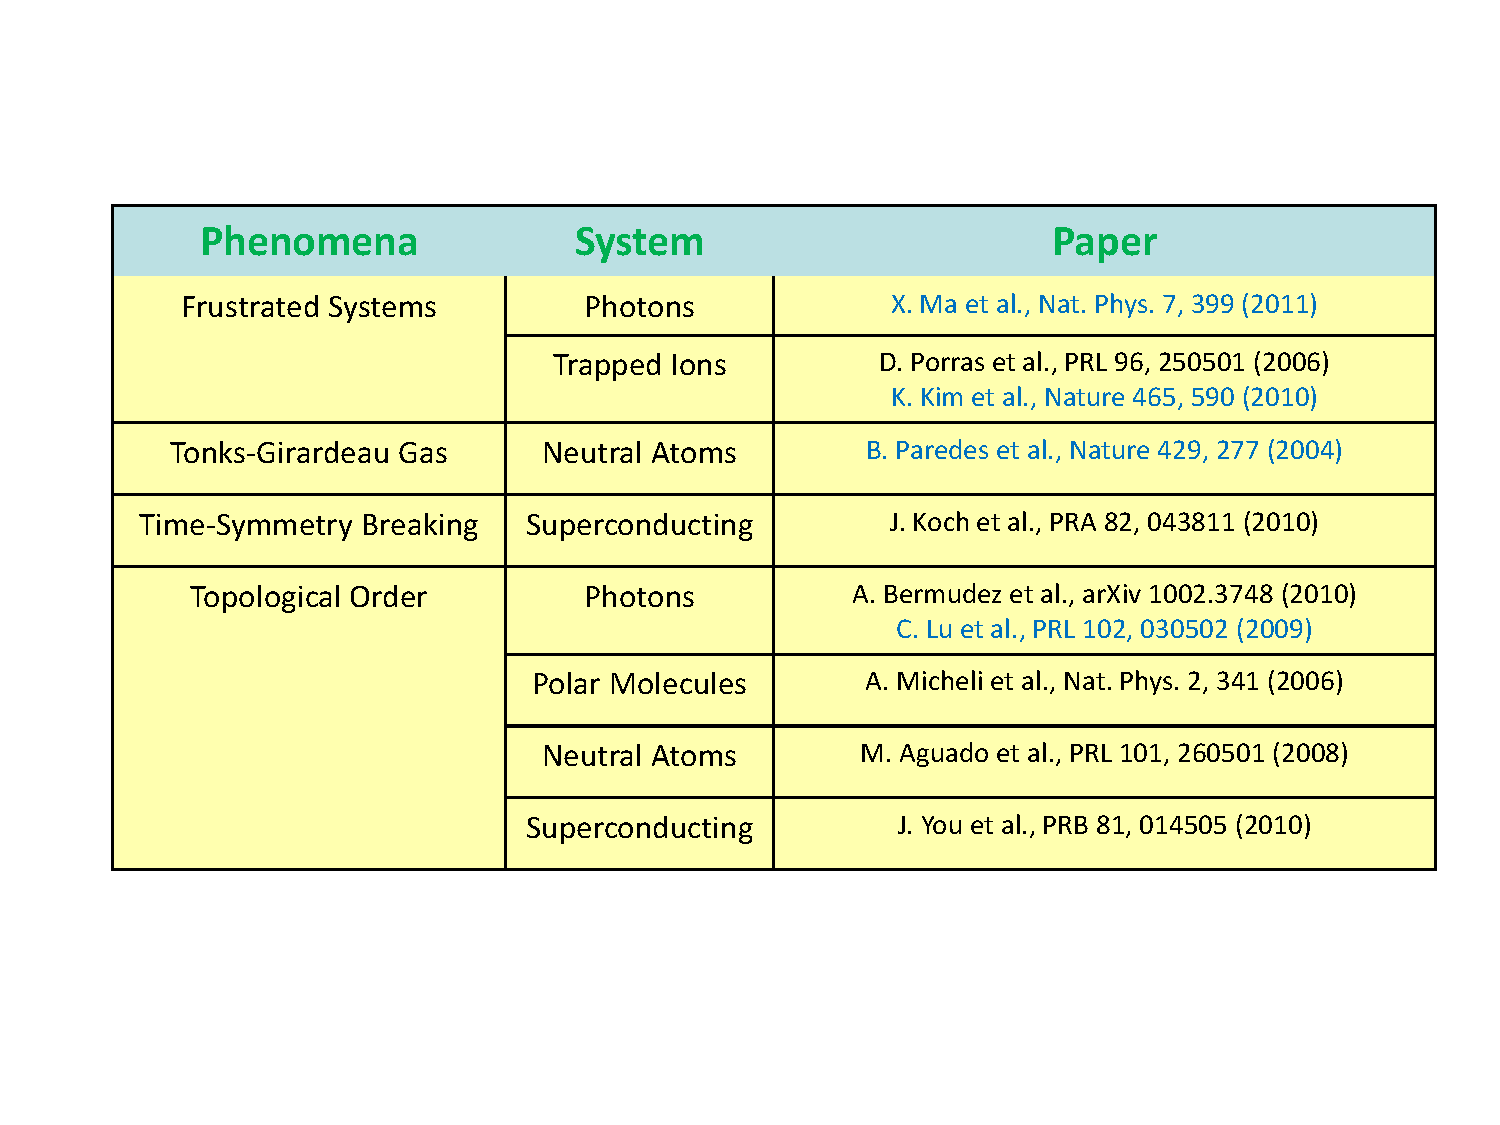
\includegraphics[width= 0.8\columnwidth]{figures/simcondense4.pdf}
              \caption{量子模拟在凝聚态物理中的应用(下)。蓝色字体为实验进展,黑色字体为理论进展。
              }
              \label{supersim}
            \end{center}
\end{figure}

  \subsection{高能物理}

量子模拟另外一个应用是在高能物理领域。第一次关于利用量子模拟研究相对论量子系统,例如规范场和Dirac费米子等的工作在1998年被提出\cite{energy1}
后来,陆续有其他一些模拟高能物理的理论和实验出现,比如如何建立2+1 Dirac振子和Jaynes-Cummings模型的映射\cite{dirac1},3+1维度模拟Dirac方程\cite{dirac2,dirac} ,最近扩展到了利用离子阱\cite{energy2}及光晶格\cite{energy3}研究外磁场中的Zitterbewegung。

模拟晶格规范理论也是量子多体中的困难问题之一。用DQS模拟晶格规范理论在Byrnes和Yamamoto的文章中已被详细讨论\cite{energy4},他们证明可以把$U(1), SU(2), SU(3)$中的晶格规范哈密顿量算符写成自旋算符的形式,因此就可以在DQS上模拟。该方案中需求的逻辑门数量和模拟晶格的总数呈一个线性到二次函数之间的某种函数关系,因此
是有效的。同时,初始化和测量和晶格尺度的关系也是类似的。

光晶格则可以用来作为AQS模拟ring-exchange模型\cite{energy5,energy6},其哈密顿量为
\begin{equation}\label{supersim}
 H_{RE} = K\sum_{plaquettes}(b_1^{\dagger}b_2b_3^{\dagger}b_4+b_4^{\dagger}b_3b_2^{\dagger}b_1-n_1n_2-n_3n_4)。
\end{equation}
这个哈密顿量可以用一个含两个态的原子实现:一个被囚禁在四角晶格内并用Bose-Hubbard模型实现,另一个被囚禁在平面晶格内。利用这个模型我们还可以模拟
一系列的强耦合哈密顿量,并且研究强关联系统的性质。
\begin{figure}[htbp]
            \begin{center}
              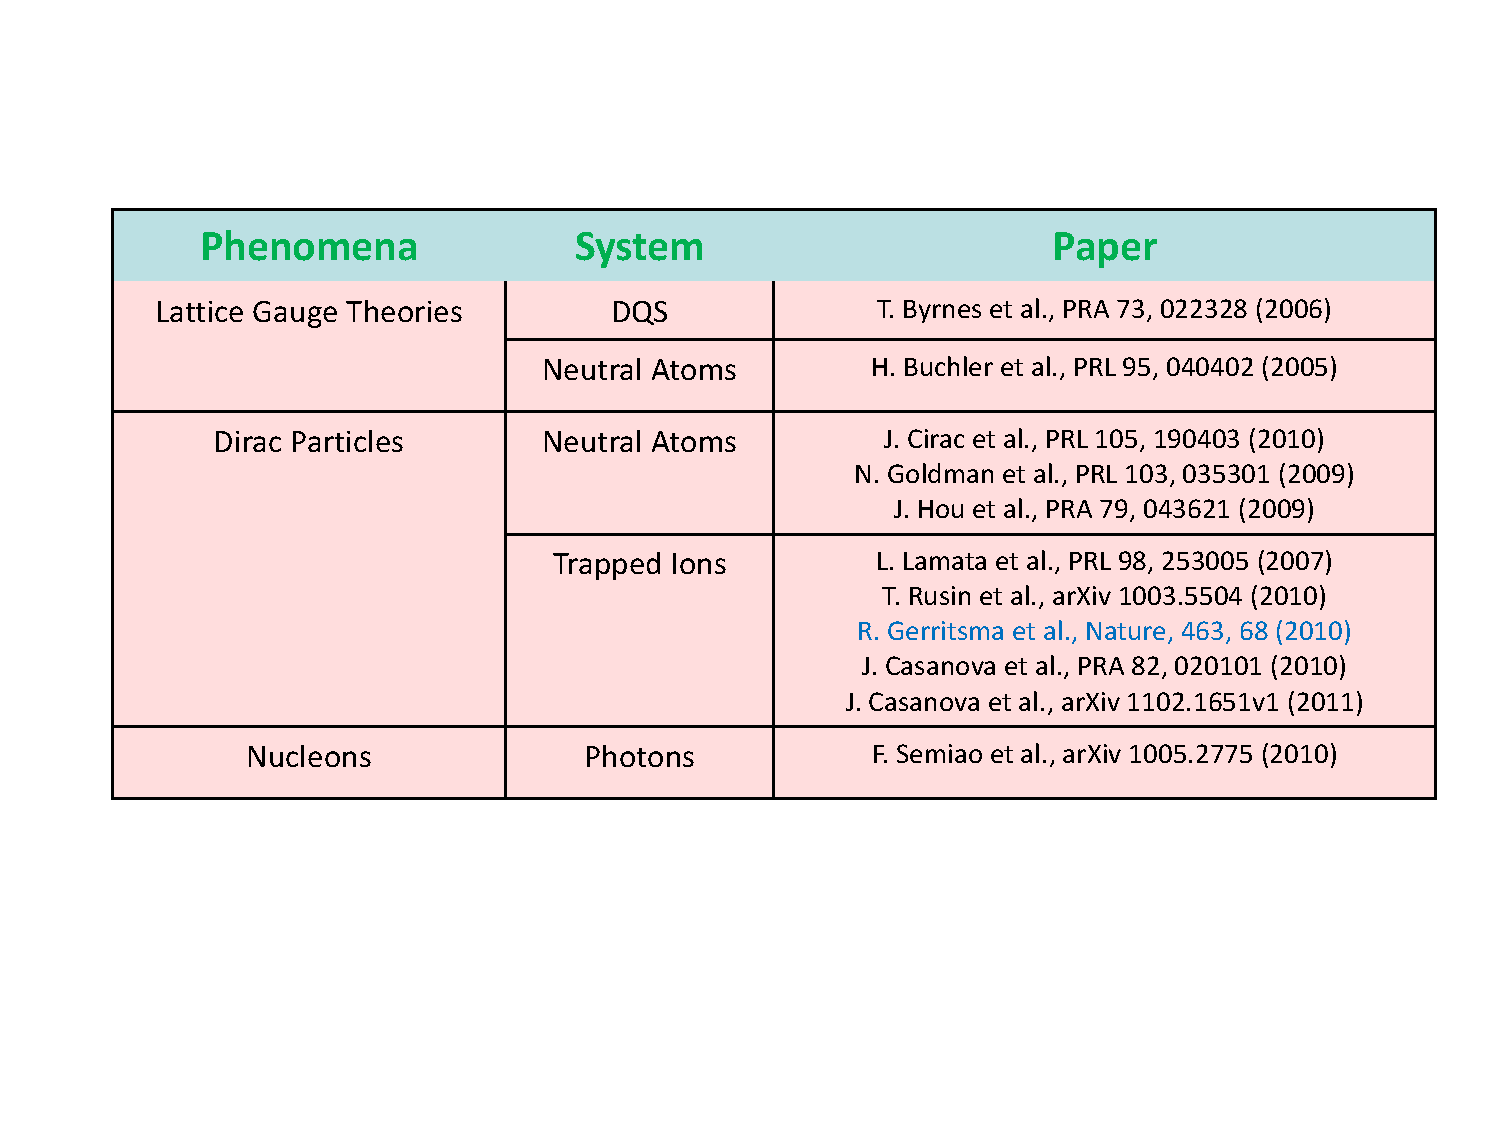
\includegraphics[width= 0.8\columnwidth]{figures/simhigh.pdf}
              \caption{量子模拟在高能物理中的应用。蓝色字体为实验进展,黑色字体为理论进展。
              }
              \label{simhigh}
            \end{center}
\end{figure}

此外,其他的方案还有利用光学体系模拟核子\cite{energy7}以及$O(3)$非线性介子模型\cite{energy8}等。

  \subsection{宇宙学}

量子模拟在万有引力理论以及宇宙学模型。例如利用BEC中的声波研究宇宙时空结构中的标量场\cite{cosmic},通过改变粒子内的耦合可以实现这个模拟过程。虽然
该方案在实验上很有挑战性,但它开辟了一条研究宇宙学的新道路。后来,利用AQS在离子阱中模拟宇宙粒子产生的方案\cite{cosmo1}及研究宇宙时空中的量子场效应的方案\cite{cosmo2}陆续出现。
利用AQS的方式,很有可能测试一些理论上有预言,但实验上尚未被观测到的现象,例如离子阱中的声子激发观测类Unruh效应\cite{unruh},或者光晶格中的中性原子
模拟Schwinger效应\cite{cosmo3},甚至Hawking辐射\cite{cosmo4,cosmo5}。

\begin{figure}[htbp]
            \begin{center}
              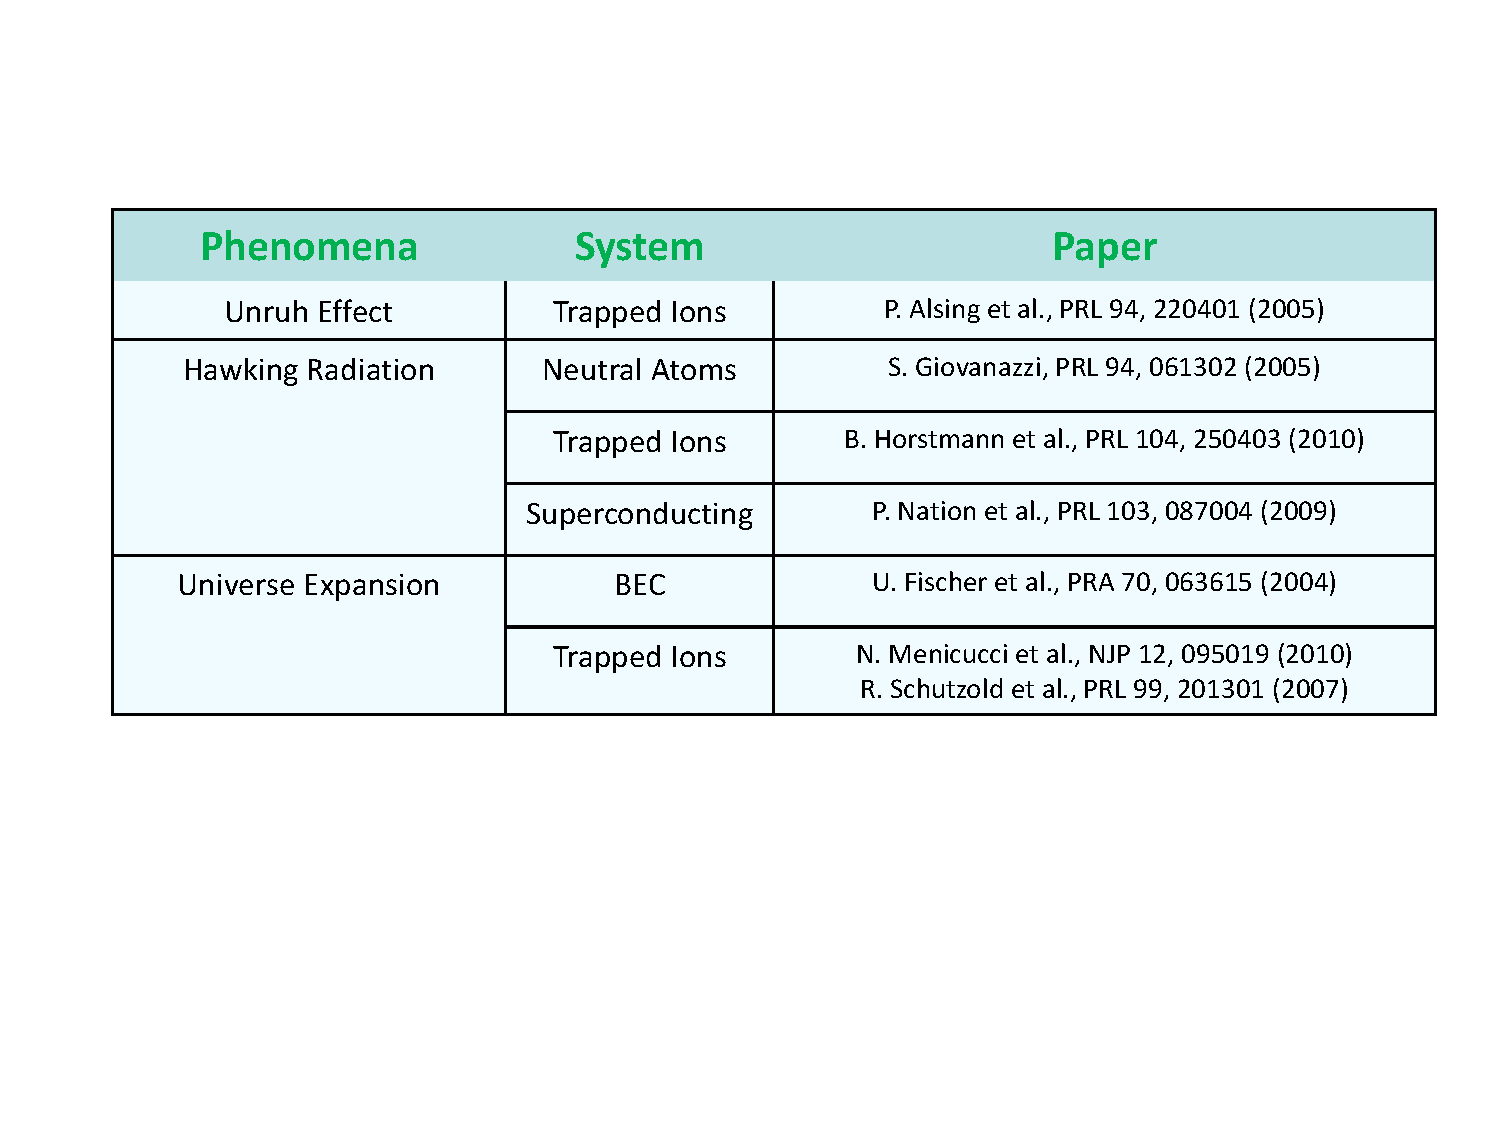
\includegraphics[width= 0.8\columnwidth]{figures/cosmic.pdf}
              \caption{量子模拟在宇宙学中的应用。蓝色字体为实验进展,黑色字体为理论进展。当然目前没有任何实验进展。
              }
              \label{cosmic}
            \end{center}
\end{figure}

 \subsection{原子物理}

原子物理及量子光学中最重要的模型之一是Jaynes-Cummings哈密顿量电磁场的单量子模式和两能级原子之间的相互作用,其形式为
\begin{equation}\label{supersim}
 H_{JC} = i\hbar g_0(a^{\dagger}\sigma_{-}-a\sigma_{+}),
\end{equation}
$g_0$是原子和场的耦合常数,$a^{\dagger}(a)$为玻色产生(湮灭)算符,而$\sigma_{+}(\sigma_{-})$为升(降)算子。

超导线路是非常适合实现Jaynes-Cummings哈密顿量模型的\cite{atomsim1}。超导线路非常适合模拟原子物理是因为
其行为非常类似于原子,或者叫“模拟原子”。和自然的原子相比,超导线路不需要采用可见光或微波
技术激发电子,而是通过电流、电压驱动这种激发过程。超导线路可以被特殊设计,比如极大的耦合项或者特定的跃迁频率,因此相对
真正的原子更有优势。在原子物理的现象中,除了模拟量子光学\cite{supersim5},超导线路还可以模拟边带冷却和科林斯王冷却(源于希腊神话的故事)\cite{atomsim2},
Landau-Zener-Stuckelberg干涉仪\cite{atomsim3}, Einstein-Podolsky-Rosen实验\cite{super2}等。

\begin{figure}[htbp]
            \begin{center}
              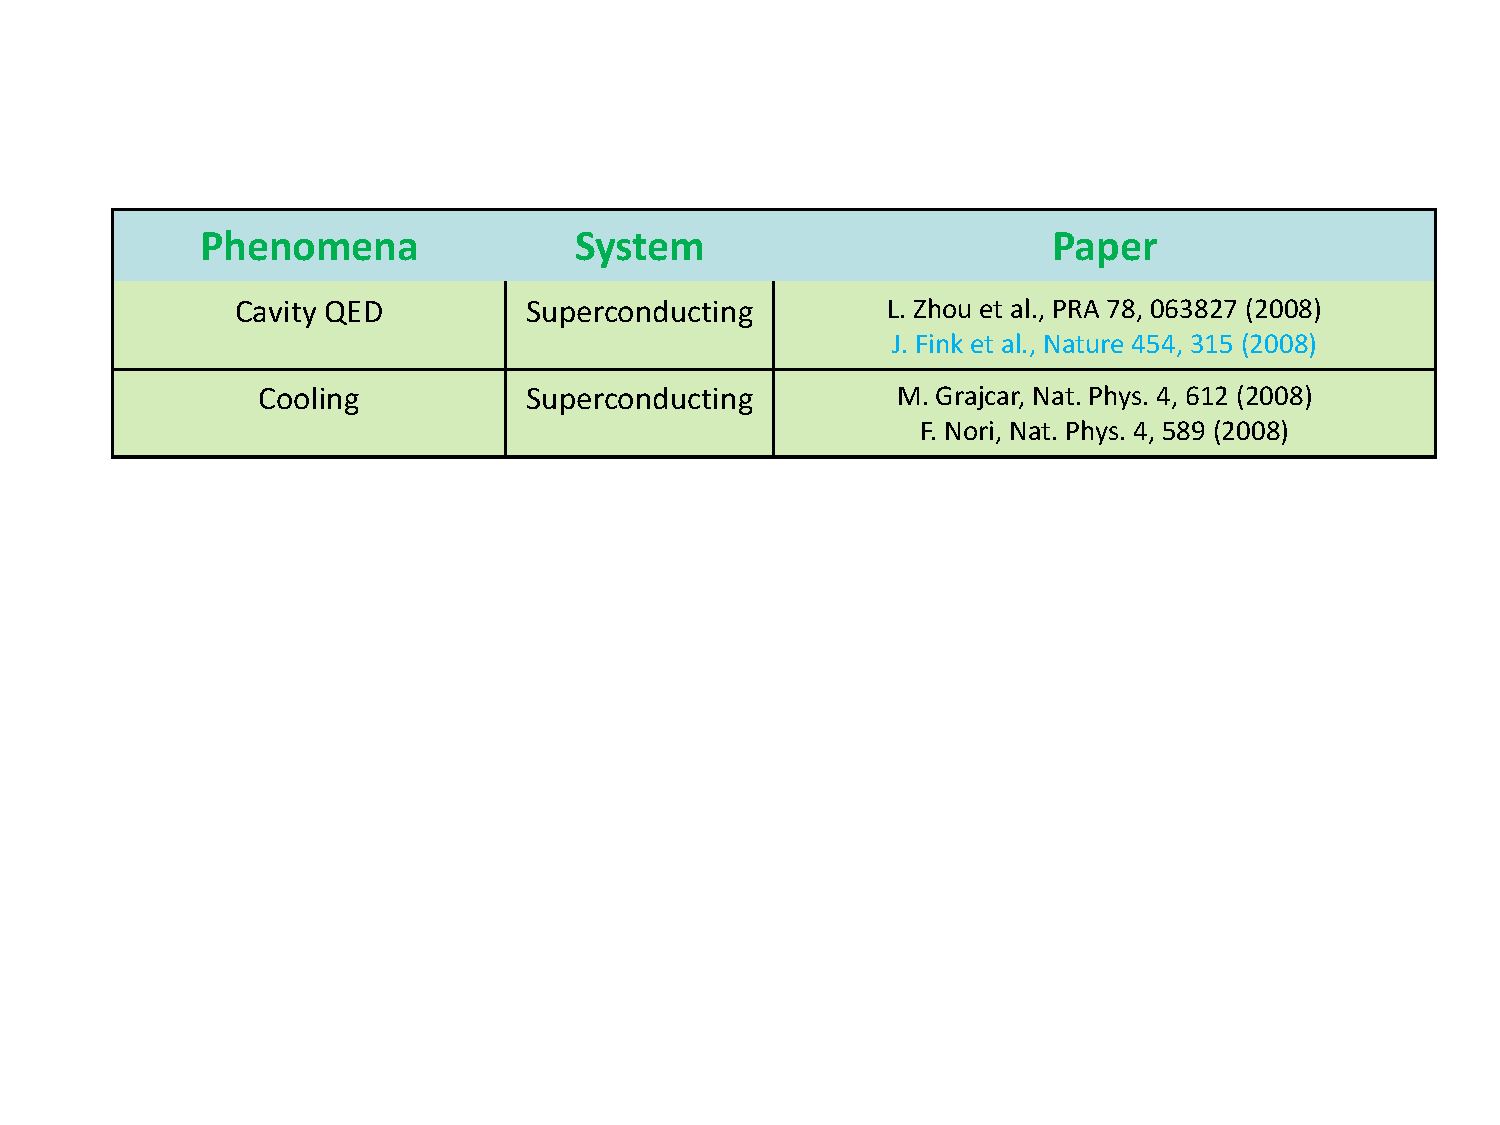
\includegraphics[width= 0.8\columnwidth]{figures/atomsim.pdf}
              \caption{量子模拟在原子物理中的应用。蓝色字体为实验进展,黑色字体为理论进展。
              }
              \label{atomsim}
            \end{center}
\end{figure}


 \subsection{量子化学}

量子模拟对量子化学也可以有很多贡献\cite{chem1}。在热反应速率常数的计算中\cite{chem2},首先把初态制备到所有位置本征态的等概率叠加态上,利用量子傅里叶变换
实现幺正演化,最后施加一系列测量并得到能量谱和幅度。该算法是多项式复杂度的,而在经典上要计算这个问题是指数复杂度的。

Aspuru-Guzik等人也提出可以利用DQS模拟分子的静态能级\cite{Alan_first}和动力学反应\cite{Polynomial_time_algorithm}。在模拟分子能级的过程中,qubit的数目是随着基矢数目的
增加呈线性增长的,而逻辑门的数目是多项式增长的,并证明利用几十个qubit我们就可以超越经典计算的结果。而在动力学模拟的过程中,该方案的复杂度也是多项式的。
这两个方案均已在实验上实现\cite{optics_static,static,dynamical}。这部分内容将在本论文的后面详细叙述,此处暂不作详细讨论。

用AQS也是可以模拟化学反应的。用可以视作“模拟原子”的量子点我们可以模拟多种化学反应\cite{reaction},最近还提出波导上的极冷原子也可以模拟化学反应过程\cite{chem3}。

\begin{figure}[htbp]
            \begin{center}
              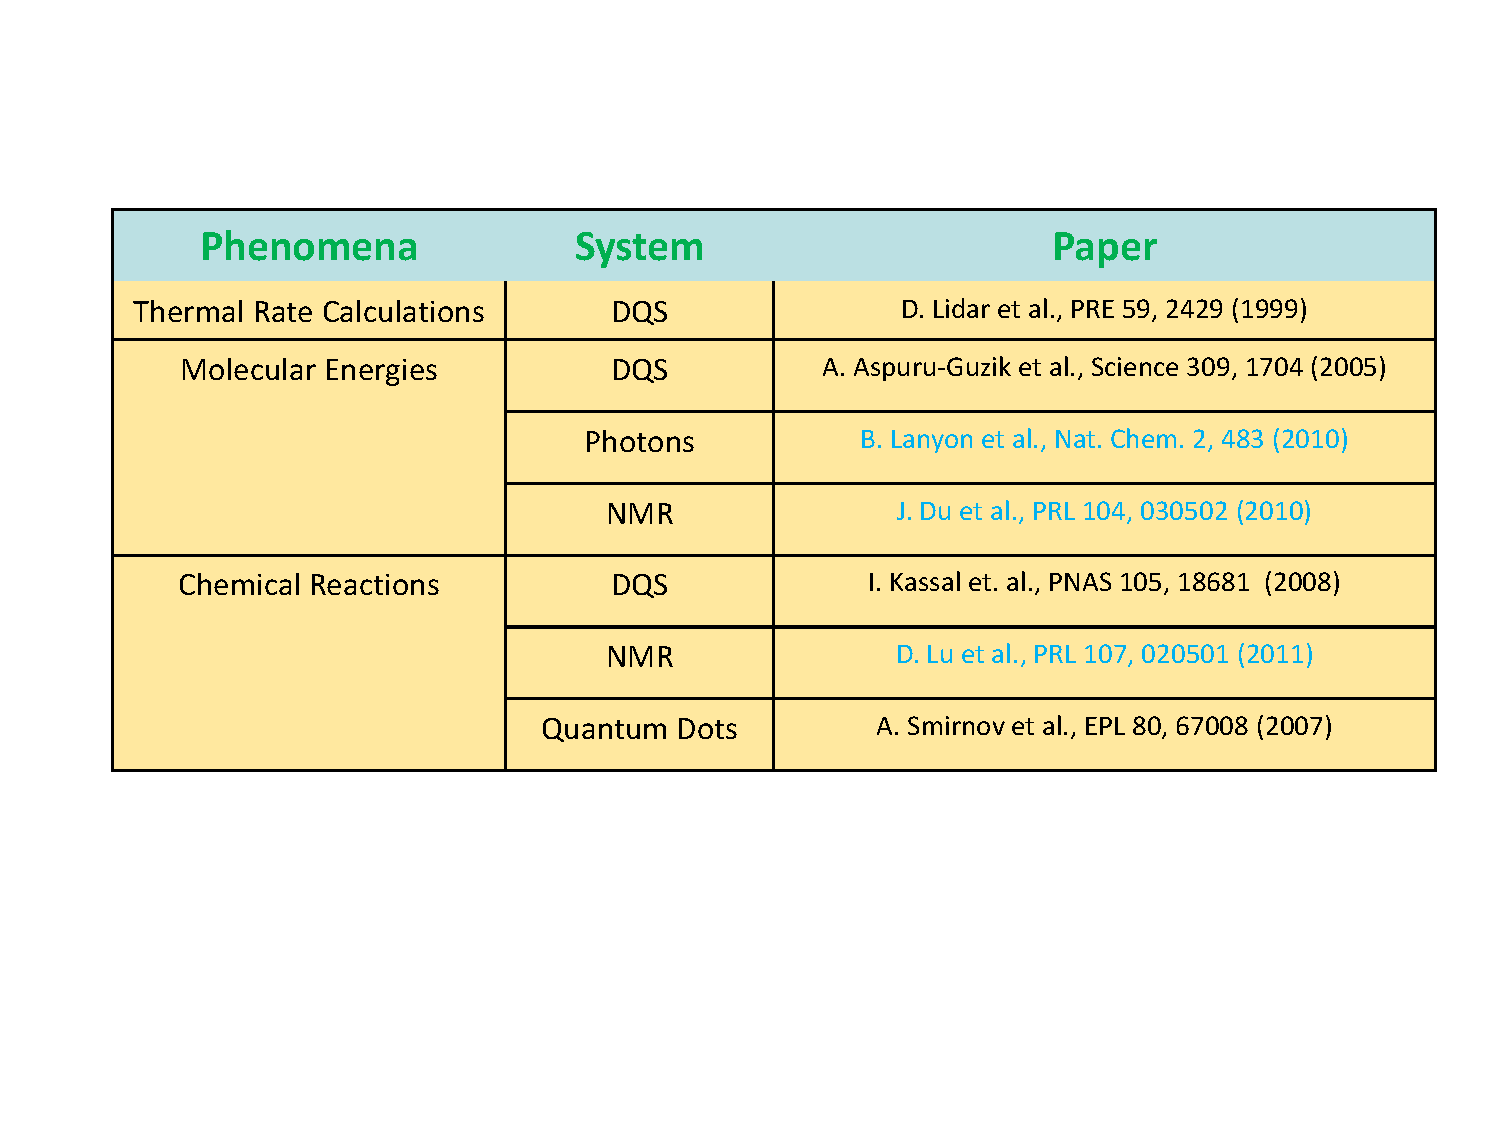
\includegraphics[width= 0.8\columnwidth]{figures/simchem.pdf}
              \caption{量子模拟在量子化学中的应用。蓝色字体为实验进展,黑色字体为理论进展。
              }
              \label{simchem}
            \end{center}
\end{figure}

 \subsection{开放系统}

模拟开放系统的动力学行为比封闭系统复杂很多,因为求解Lindblad方程需求的资源是求解薛定谔方程的二次方关系。模拟量子开放系统主要有两条路径:第一是通过利用实验
体系中天然的退相干机制\cite{Lloyd,deco}。第二条是利用封闭量子系统研究开放量子系统,例如利用驱动谐振子作为量子模拟器我们可以模拟非马尔科夫的阻尼谐振过程\cite{open1}。
模拟开放系统动力学机制的一般方法可以参见Bacon等的文章\cite{open2}。

\subsection{量子混沌}

DQS的一个应用就是用几个qubit研究简单量子映射的动力学过程,而量子面包师映射(quantum baker's map)是量子混沌中的典型问题。如果用量子模拟我们可以有效地解决这类问题,并在NMR\cite{chaos2}和线性光学\cite{chaos1}上已经被证实。
另外一个例子是kicked Harper模型\cite{chaos3}。在文章中的条件下,量子算法可以提供指数的加速,而且只用八个qubit就可以表现出非常有趣的性质。

\subsection{其它}

量子模拟的应用还有很多,比如利用DQS模拟薛定谔方程\cite{energy1,others1},量子热机\cite{others2,others3},量子热动力学\cite{others4}。现在量子模拟在物理和化学领域
都有非常多潜在的应用。利用量子模拟我们既可以解决一些经典上难以处理的问题(比如上面提到的凝聚态物理中的很多的问题),也可以实现一些实验非常困难甚至根本不能
做实验的难题(比如上面提到的高能物理和宇宙学中的一些问题)。随着技术的进步,肯定会有更多的学科希望加入到量子模拟的大军中来,也肯定会有更多新的应用将被展示。

\begin{figure}[htbp]
            \begin{center}
              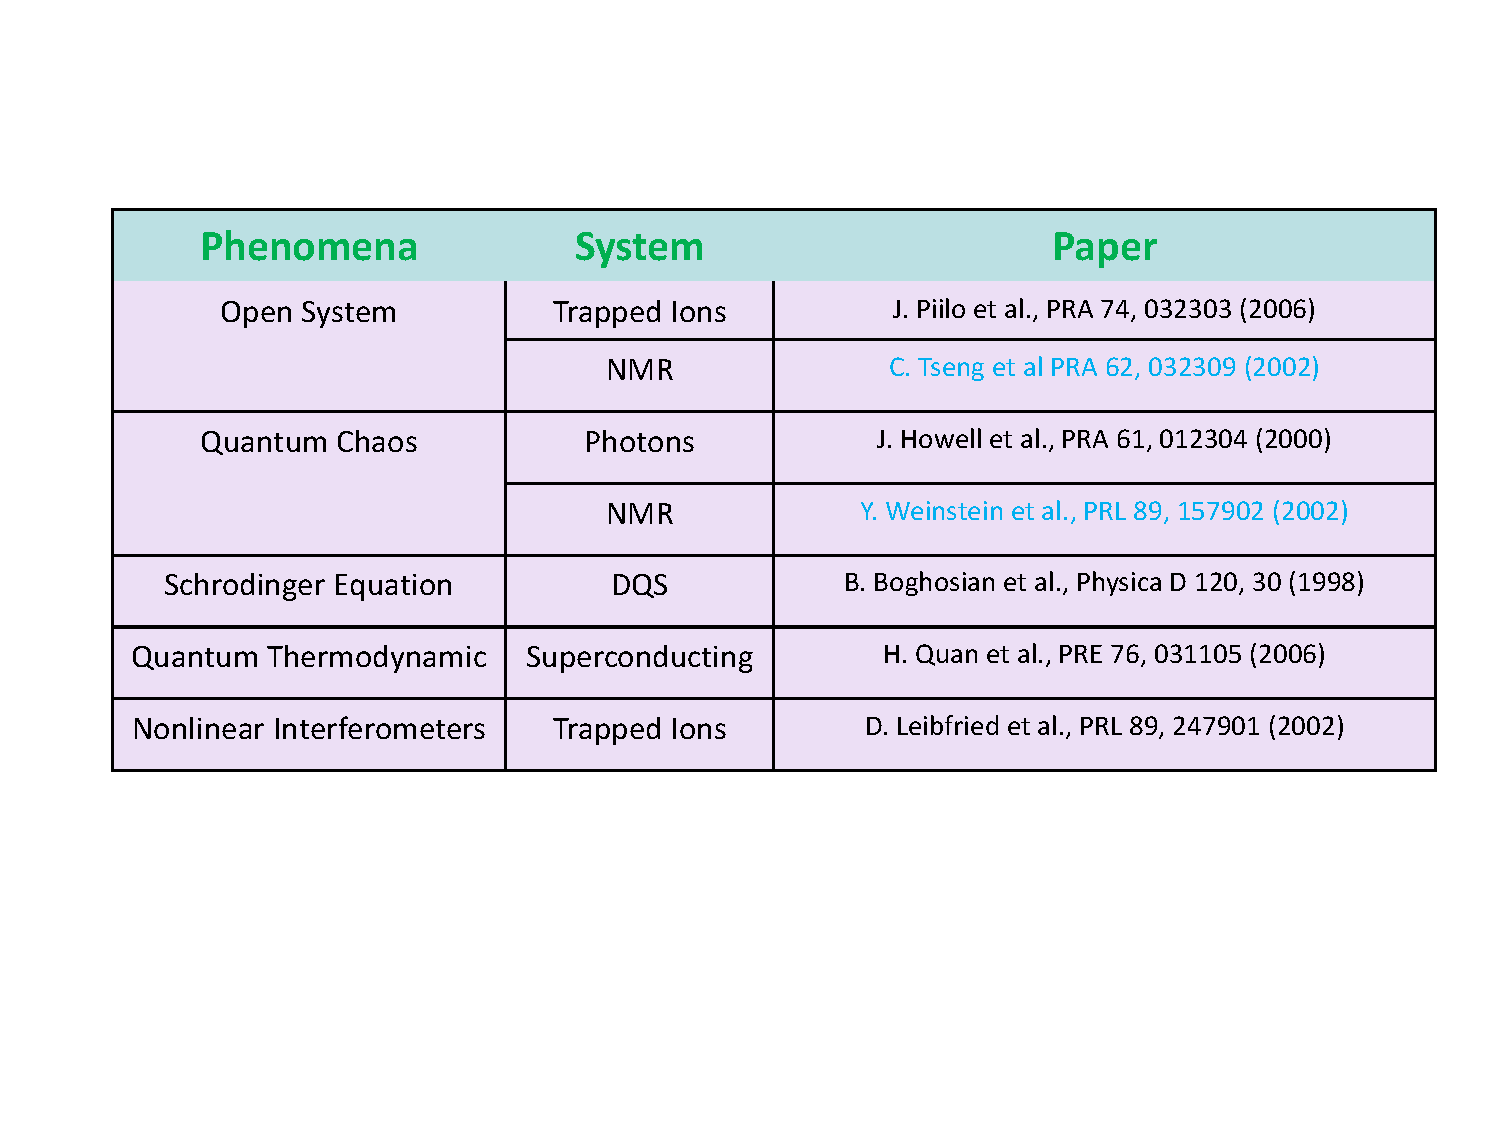
\includegraphics[width= 0.8\columnwidth]{figures/simother.pdf}
              \caption{量子模拟的一些相对“非主流”的应用。蓝色字体为实验进展,黑色字体为理论进展。
              }
              \label{simother}
            \end{center}
\end{figure}

\section{量子模拟的展望}

最近关于量子模拟的理论和实验进展让我们有理由期待在不远的未来一些特殊的量子模拟器能被建成。当然,理论和实验上还是有些问题要先克服的。

从理论的角度看,退相干和相干操控的研究依然是重点,同时对每个量子模拟器给出实验资源需求的估计也是必须的。量子模拟的新应用也是非常值得期待的,毕竟目前大多数的
方案和实验都在凝聚态物理上。

从实验的角度看,和量子计算机的要求类似,操控和可扩展性依然是两大难题。除了光晶格中的冷原子,其他的量子模拟目前还很难操控大的qubit阵列。尽管如此,光晶格中qubit
的单独控制和读出又是非常困难的,对其他体系这可能又不是一个很难的问题。目前还有绝热量子模拟的概念被提出\cite{adiaqs},这种新型的量子模拟器可能在实验上比基于逻辑门的DQS要简单。


\section{小结}

本章的主要内容是量子模拟。除了详细介绍量子模拟的概念及思想之外,本章也希望作为一个迄今为止比较完善的量子模拟资料库来使用,这对以后实验寻找新的、可行的量子模拟
方案有极大的便利之处。

\begin{figure}[htbp]
            \begin{center}
              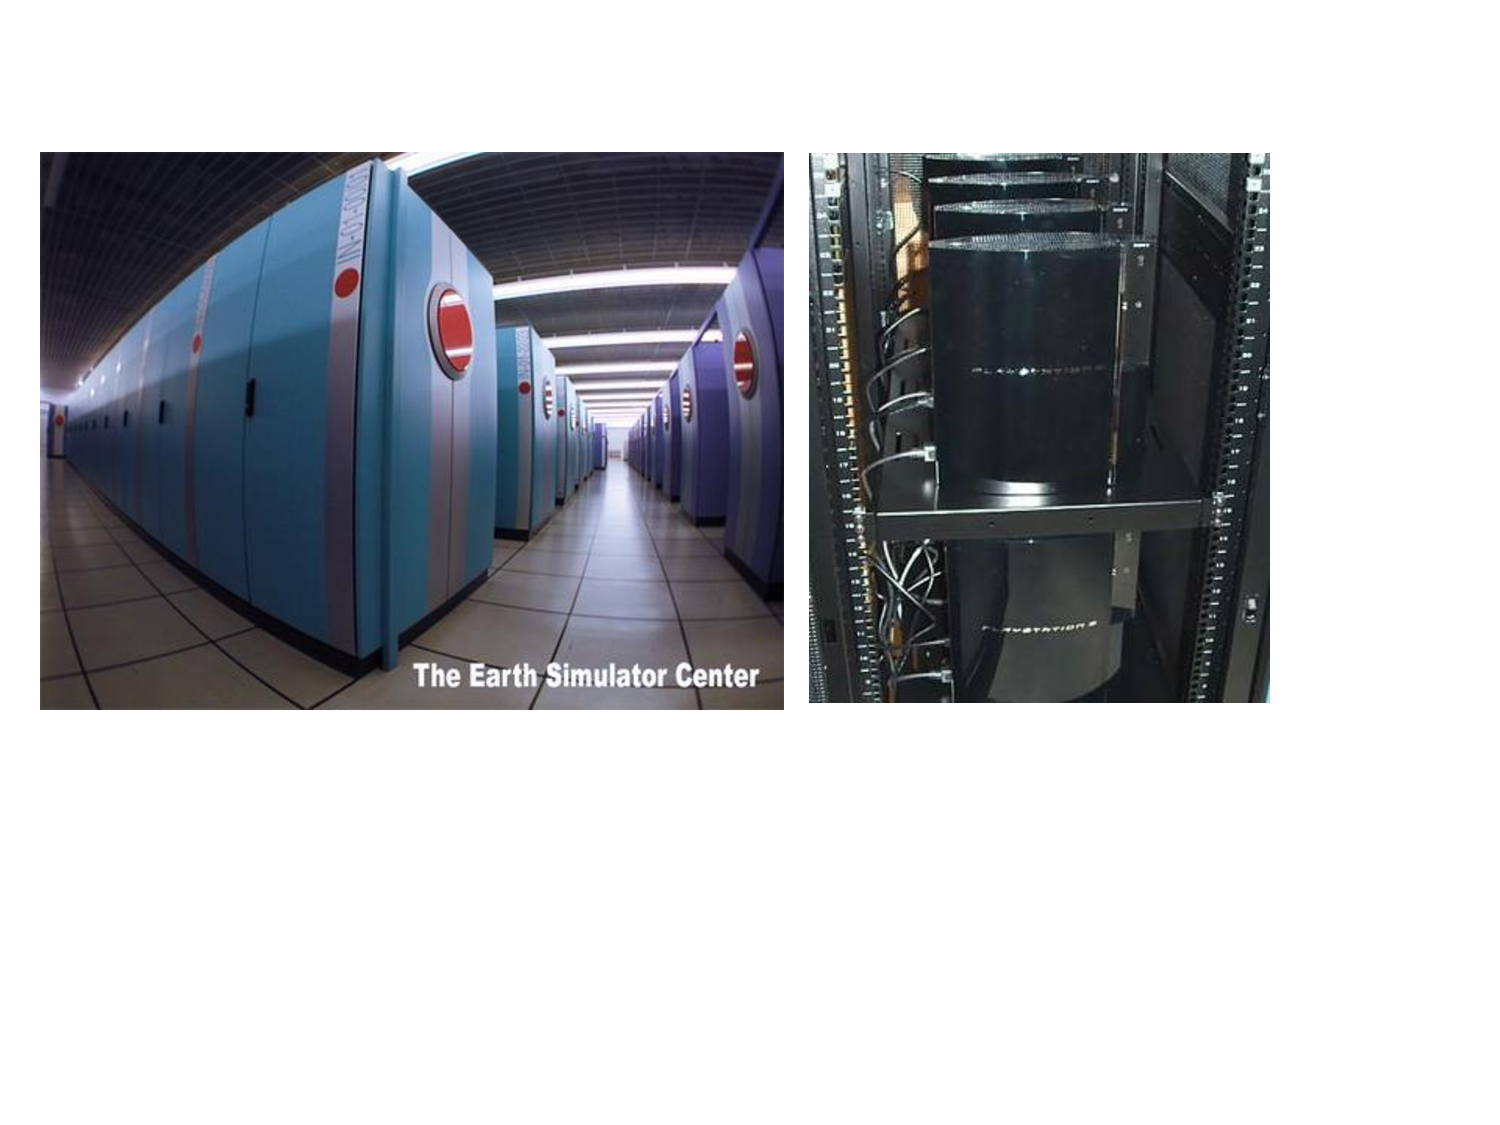
\includegraphics[width= 0.8\columnwidth]{figures/nec.pdf}
              \caption{(左) 日本电气公司(NEC)2002年开发的超级计算机“地球模拟器”。(右) PlayStation3被北卡罗来纳州立大学教授Frank Mueller做成阵列来跑计算,足见其计算能力之强,但离谣传的模拟地球依然差距不小。
              }
              \label{nec}
            \end{center}
\end{figure}

其实人类有一个很大的愿望就是成功模拟地球。早在2002年,日本电气公司(NEC)就为它研制的当时地球上最强大的超级电脑(比之前最快的IBM公司的ASCI White-Pacific快近五倍) 取了一个非常霸气的名字:地球模拟器(Earth Simulator)。当时这台电脑主要用于分析气候变化,当然不可能做到真正模拟地球上万物的演化。后来又有谣传说索尼(Sony)公司的新一代游戏主机PlayStation3可以强大到模拟地球,还一度愈演愈烈。
后来证实这只是一个半吊子的中日文翻译的问题。虽然目前看还不可能,但人类追逐梦想的脚步是从未停息的,而模拟地球应该是一个非常伟大的梦想。通过本章的介绍,我觉得我们可以怀有这种梦想:
量子模拟不仅只能用在凝聚态,高能物理,宇宙学,原子物理,量子化学上,它或者有着更加广阔的,更加不可思议的应用。当然目前我们最需要的依然是理论和实验上继续把这套思想完善下去,先开启“多个世界”的可能性。 
  
\chapter{核磁共振量子计算}

1938年,Rabi发现处于磁场中的原子核会沿着磁场方向呈正向或反向平行排列,而在施加射频场之后,
这些原子核的自旋方向会发生翻转,这就是著名的拉比振荡(Rabi oscillation) \cite{rabi}。Rabi振荡是人类关于原子核与外加磁场和射频场的相互作用现象的最早认识,而Rabi本人也赢得了1944年的诺贝尔物理奖。1946年,
Bloch和Purcell则发现处于外磁场中的特定核自旋,比如$^1$H, $^{31}$P等,会吸收特定频率的射频场能量,这是人类对于核磁共振最初的认识\cite{nmrhistory},两人也分享了1952年的诺贝尔物理奖。

后来,人们发现核磁共振(Nuclear Magnetic Resonance, 以后均简称为NMR)现象有非常多的应用。在化学上,NMR可以用来解析分子结构,从最早期的简单一维氢谱到后来的$^{13}$C谱,二维谱等高级谱图,NMR可以分析的分子结构
越来越复杂。在化学领域,NMR谱与紫外光谱、红外光谱和质谱并称为“四大名谱”,而我国的高中化学教材里也加入了NMR介绍的章节。除了化学上,医学家们也发现人体中水分子的
氢原子可以产生核磁共振现象,可以通过这一现象获取人体内水分子的分布信息,进而精确绘制人体的内部结构,这也就是目前在医学上广泛应用的核磁共振成像技术(MRI)。

另一方面,超过50年的NMR技术的发展成熟使人们早已可以精确操控NMR中耦合起来的两能级量子系统。在量子计算的概念提出后,NMR也自然的成为非常有潜力的实验验证量子计算
方案的平台,并一直作为各个量子计算潜在方案中操控比特数最多,量子算法最复杂的一个方案而被广泛研究,而在NMR量子计算中发展出的许多技术不仅可以应用在NMR在其他领域的研究上,也
经常被借鉴于其他量子计算平台。在本章中,我们将从NMR如何进行量子计算讲起,包括内部和外部哈密顿量形式,
脉冲技术和逻辑门操作,以及初态制备和测量读出等实现量子计算机的各方面要求。通过这些内容,我们会具体分析NMR量子计算的利弊。而在本章的最后,我们将给出如何利用并不常见的强耦合体系NMR做量子计算,并
给出实验上利用四比特强耦合体系进行143大数分解的实例。

\section{NMR系统}

对于NMR系统最简单的描述就是内部系统哈密顿量与外部控制哈密顿量联合进行动力学演化的过程。系统哈密顿量给出在静磁场中单个的,或者耦合起来的核自旋的能量形式,而控制哈密顿量
则是来自于以系统的共振频率外加的射频脉冲。一般来说,NMR中我们常用的是旋转坐标系,在这个坐标系里考虑问题会相当简单。

\subsection{内部哈密顿量}

在一个沿$\hat{z}$方向的静磁场$B_0$中,自旋1/2的粒子(在本论文中,我们不考虑更高阶的自旋)的动力学演化将被其系统哈密顿量主导
\begin{equation}\label{static}
 H_{0} = -\hbar \gamma B_0 I_z = -\hbar \omega_0 I_z = \left(
                                                         \begin{array}{cc}
                                                           -\hbar \omega_0/2 & 0 \\                                                           0& \hbar \omega_0/2 \\
                                                         \end{array}
                                                       \right),
\end{equation}
其中$\gamma$是原子核的旋磁比,$\omega_0/2 \pi$是Larmor频率,$I_z$是$\hat{z}$方向的核自旋算符。$I_x, I_y, I_z$和Pauli算符有如下的对应形式
\begin{equation}\label{static}
 \sigma_x = 2I_x,  \sigma_y = 2I_y,  \sigma_z = 2I_z ,
\end{equation}
并且
\begin{equation}\label{static}
 \sigma_x \equiv \left(
                   \begin{array}{cc}
                     0 & 1 \\
                     1 & 0 \\
                   \end{array}
                 \right);
  \sigma_y \equiv \left(
                   \begin{array}{cc}
                     0 & -i \\
                     i & 0 \\
                   \end{array}
                 \right);  \sigma_z \equiv \left(
                   \begin{array}{cc}
                     1 & 0 \\
                     0 & -1 \\
                   \end{array}
                 \right).
\end{equation}

对于这种系统哈密顿量的形式更直观的理解是,本征态$\left\vert  0 \right\rangle$(有时候也叫$\left\vert  \uparrow \right\rangle$)的能量本征值将比
本征态 $\left\vert  1 \right\rangle$(有时候也叫$\left\vert  \downarrow \right\rangle$) 小$\hbar \omega_0$,这种能量劈裂叫做Zeeman劈裂。

\begin{figure}[htbp]
            \begin{center}
              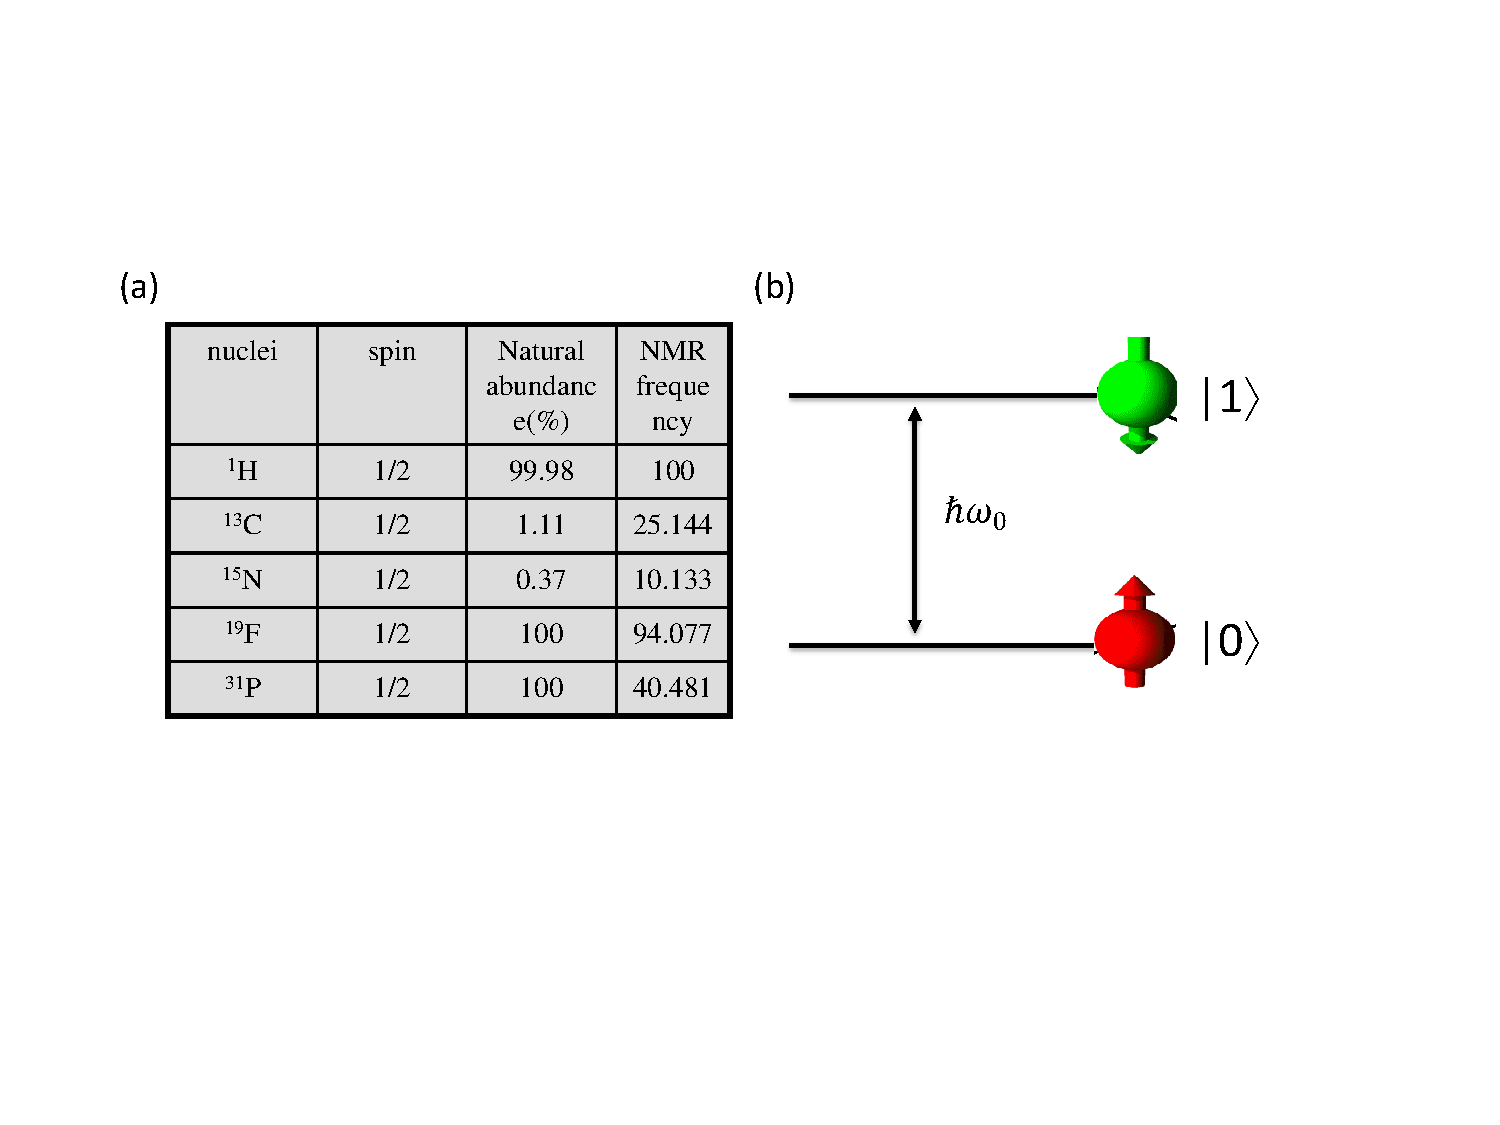
\includegraphics[width= 0.8\columnwidth]{figures/spinhalf.pdf}
              \caption{(a) 几种常用的自旋1/2粒子的天然丰度及Larmor频率。(b) 自旋 1/2粒子的能级图。
              }
              \label{spinhalf}
            \end{center}
\end{figure}

我们可以近似地把时间演化算子$U=e^{-iHt}$理解为一个矢量在Bloch球上绕着$\overrightarrow{B_0}$的进动过程。方便起见,我们把Bloch球的$\hat{z}$轴定义为$\overrightarrow{B_0}$
方向,而$\left\vert  0 \right\rangle$沿着$+\hat{z}$方向,$\left\vert  1 \right\rangle$沿着$-\hat{z}$方向。对于液体NMR的情况来说,$B_0$的典型值为5-15T,导致进动频率$\omega_0$的大小为几百MHz,也就是射频的范围。

不同种类的核自旋可以很容易地辨别,因为它们的旋磁比$\gamma$不同,从而拥有相差很远的Larmor频率。对于相同的原子核来说,它们也有不同的频率,叫做化学位移。化学位移来源于环绕原子核周围的电子云产生的磁场的部分屏蔽作用,该屏蔽的大小取决于原子核周围的电子分布,因此具有不同核外电子环境的原子核
具有不同的化学位移。典型的化学位移范围依赖于不同的原子核,比如对$^1$H来说,它的范围约为10ppm(百万分之一,NMR常用的频率单位),对$^{13}$C和
$^{19}$F则约为200ppm。在静磁场$B_0$的大小为10T时,化学位移的值大概从几kHz到数十kHz,相比于Larmor频率的百万MHz的数量级来说还是非常小的。

一般来说,化学位移是空间各向异性的,要用张量来描述。在液体NMR中,由于分子间的快速滚动,各向异性的影响被平均掉了,而在固体NMR中,
各向异性表明化学位移是依赖于分子取向的,也就是和静磁场$B_0$的夹角。

不同于孤立的原子核的哈密顿量,有相互作用的原子核主要存在两种不用的相互作用机制:直接的偶极-偶极耦合以及间接的标量耦合。

(a) \emph{直接耦合}

偶极-偶极耦合的相互作用类似于两个临近的条形磁体的相互作用,它纯粹是通过空间产生相互作用的,并不需要第三方介质。该作用主要依赖于
核间矢量$\overrightarrow{r_{ij}}$,可以被如下哈密顿量形式描述
\begin{equation}\label{static}
H_D = \sum_{i<j} \frac{\mu_0\gamma_i \gamma_j \hbar}{4\pi |\overrightarrow{r_{ij}}|^3}(\overrightarrow{I^i}\cdot \overrightarrow{I^j}-\frac{3}{|\overrightarrow{r_{ij}}|^2(\overrightarrow{I^i}\cdot\overrightarrow{r_{ij}})(\overrightarrow{I^j}\cdot\overrightarrow{r_{ij}})}),
\end{equation}
其中$\overrightarrow{I_{i}}$自旋$i$的磁化矢量。在高场情况下,该耦合形式可以近似为
\begin{equation}\label{static}
H_D = \sum_{i<j} \frac{\mu_0\gamma_i \gamma_j \hbar}{8\pi |\overrightarrow{r_{ij}}|^3}(1-3cos^2\theta_{ij})(3I_z^i I_z^j-\overrightarrow{I^i}\cdot\overrightarrow{I^j}),
\end{equation}
$\theta_{ij}$是$B_0$和$\overrightarrow{r_{ij}}$的夹角。当化学位移之差$|\omega_0^i-\omega_0^j|$比耦合强度大很多时,
耦合项中的横向分量可以被忽略掉,$H_D$可以进一步被简化为
\begin{equation}\label{static}
H_D = \sum_{i<j} \frac{\mu_0\gamma_i \gamma_j \hbar}{8\pi |\overrightarrow{r_{ij}}|^3}(1-3cos^2\theta_{ij})I_z^i I_z^j.
\end{equation}
这个形式和下面介绍的标量耦合形式类似。

在液体NMR中,不论是分子间的偶极耦合或者分子内部的偶极耦合,由于分子的快速滚动都已经
被平均掉了。而在固体NMR中,我们可以通过施加多脉冲序列\cite{Haeberlen}或者魔角旋转技术实现类似的
简单哈密顿量形式。

(b) \emph{间接耦合}

分子中核自旋的第二种相互作用机制就是$J$耦合,或者叫标量耦合。这种相互作用机制
来源于原子间化学键中的共享电子,或者电子波函数的交叠产生的费米接触相互作用,其大小依赖于相互作用的
原子核种类,并随着化学键数目的增多而减少。典型的$J$耦合强度从几个Hz(三键或四键耦合)到几百Hz(单键耦合)不等。
$J$耦合的哈密顿量形式为
\begin{equation}\label{static}
H_J = \hbar\sum_{i<j} 2\pi J_{ij} \overrightarrow{I^i}\cdot\overrightarrow{I^j}=\hbar\sum_{i<j} 2\pi J_{ij}(I_x^iI_x^j+I_y^iI_y^j+I_z^iI_z^j),
\end{equation}
$J_{ij}$是自旋$i$和自旋$j$之间的相互作用强度。和偶极耦合的形式类似,在弱耦合近似($|\omega_0^i-\omega_0^j|\gg 2\pi |J_{ij}|$)的情况下,该形式可以化简为
\begin{equation}\label{Jappro}
H_J =\hbar\sum_{i<j} 2\pi J_{ij}I_z^iI_z^j.
\end{equation}
对于不同种类的核自旋该条件是容易满足的,而对于很多分子内的同种核自旋该条件也可能满足。

在弱耦合近似下,标量耦合作用可以用有效磁场的概念来理解:除了外加的静磁场$\overrightarrow{B_0}$外,核自旋还会感受到由邻近自旋产生的沿$\pm\hat{z}$方向的磁场。如下图所示,这个附加磁场
会使能级产生移动。当自旋$j$处于$\left\vert  0 \right\rangle$时,自旋$i$的Larmor频率将移动$-J_{ij}/2$;当自旋$j$处于$\left\vert  1\right\rangle$时,自旋$i$的Larmor频率将移动$J_{ij}/2$。

\begin{figure}[htbp]
            \begin{center}
              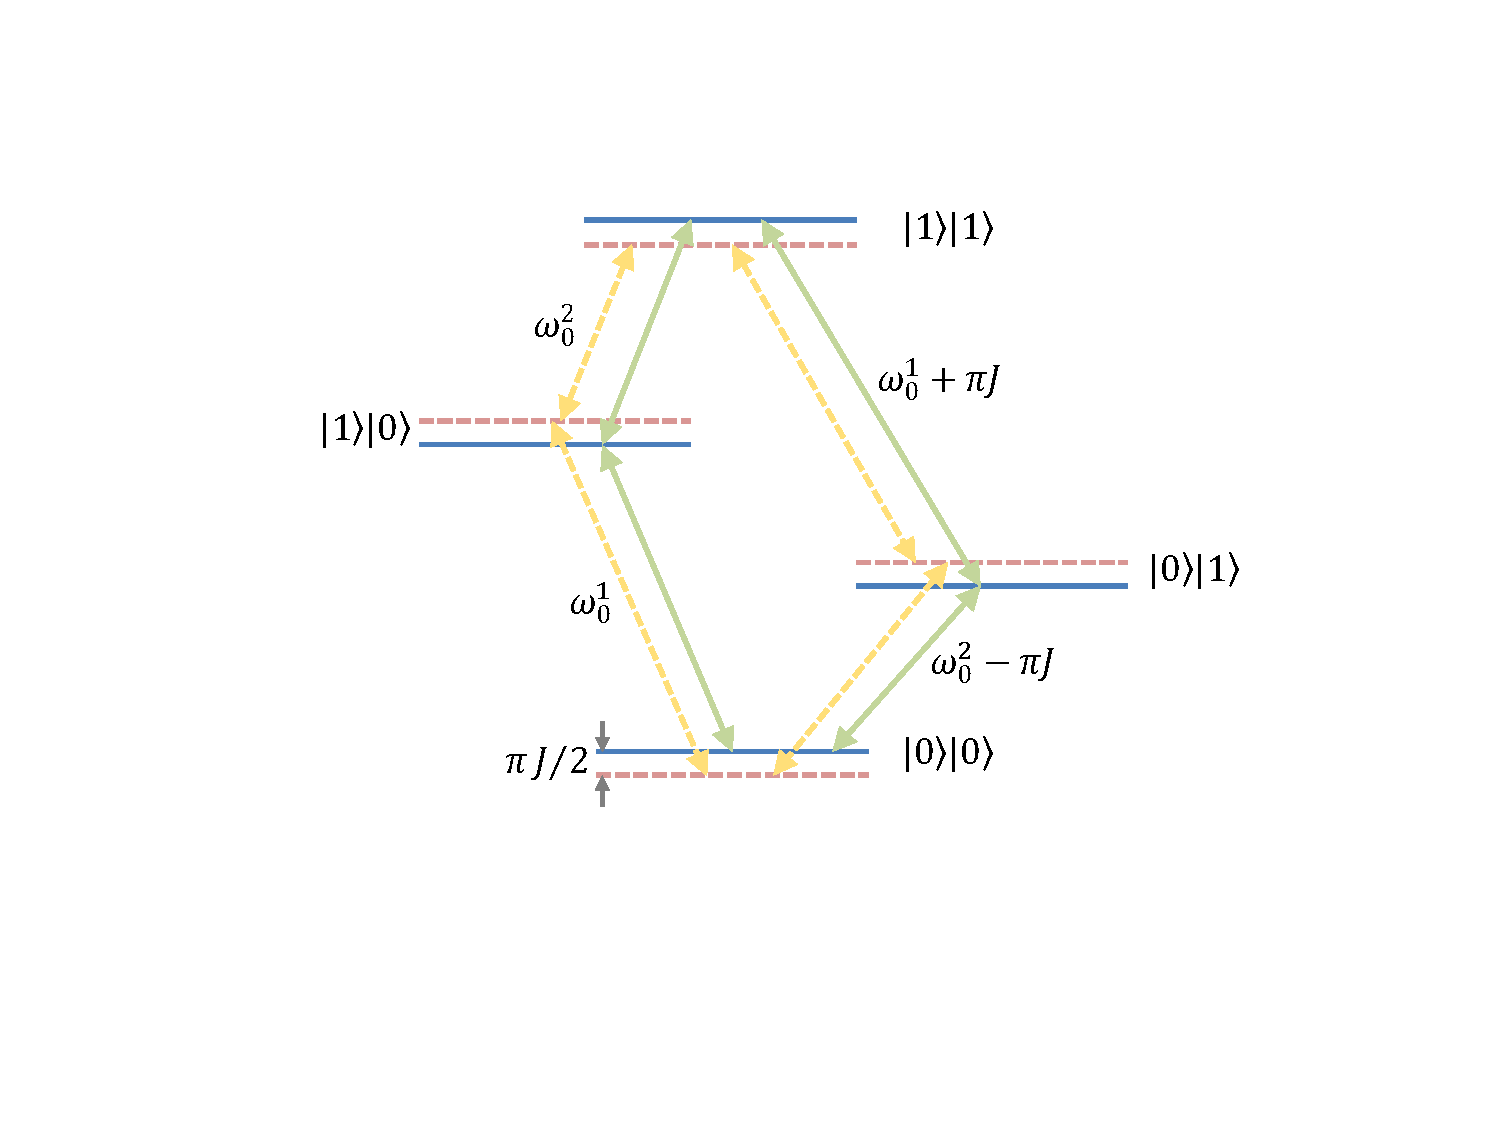
\includegraphics[width= 0.8\columnwidth]{figures/energy.pdf}
              \caption{两个未耦合的自旋的能级图(虚线)及以式\ref{Jappro}形式耦合的哈密顿量的能级图(实线)。$\hbar$已经被忽略掉。
              }
              \label{energy}
            \end{center}
\end{figure}

对于耦合起来的两个自旋系统来说,自旋$i$的频率谱线包含分离的两条,它们之间的距离为$J_{ij}$,且其中心频率
为$\omega_0^i$。两条谱线是对应于自旋$j$所处的状态的。相应地,对于三个两两耦合的自旋来说,每个自旋将
包含四条谱线,而每添加一个自旋,谱线的数目将翻倍。

所有两两耦合的大小可以通过读出不同自旋的谱线劈裂来得到。$J$耦合的符号则可以用适当的
核选脉冲序列,例如二维COSY实验\cite{sign1}或者线选脉冲的连续激发来检测。注意仅仅通过简单的NMR谱线来确定$J$耦合的符号
是不可能的。

综上所述,对于$n$个两两耦合的自旋系统来说,其最简单的哈密顿量形式为
\begin{equation}\label{aaa}
H_{sys} =-\hbar\sum_{i}\omega_0^i I_z^i+ \hbar\sum_{i<j} 2\pi J_{ij}I_z^iI_z^j.
\end{equation}
在绝大多数的NMR量子计算实验中用到的自旋系统都可以用这个哈密顿量形式来描述。

\subsection{外部哈密顿量}

本小节我们转到如何操控NMR系统上。对处于$\hat{z}$方向静磁场中的自旋1/2粒子来说,我们可以通过
外加电磁场$\overrightarrow{B_1}(t)$来进行操控。该电磁场可以加在$\hat{x}-\hat{y}$平面内的任意角度,其频率为$\omega_{rf}$,该频率的大小处于或接近自旋
的进动频率$\omega_0$。对于处于射频场中的单自旋来说,其哈密顿量形式为
\begin{equation}\label{aaa}
H_{rf} =-\hbar\gamma B_1 [cos(\omega_{rf}t+\phi)I_x-sin(\omega_{rf}t+\phi)I_y],
\end{equation}
其中$B_1$和$\phi$分别是射频场的强度和相位。射频场强度$\omega_1=\gamma B_1$的典型值为液体NMR中的小于30kHz,固体NMR中几百kHz。

对于$n$个自旋,射频场的哈密顿量为
\begin{equation}\label{aaa}
H_{rf} =-\sum_i^n\hbar\gamma_i B_1 [cos(\omega_{rf}t+\phi)I_x^i-sin(\omega_{rf}t+\phi)I_y^i].
\end{equation}
一般来说,在实验室坐标系中,外磁场在固定的、和静磁场垂直的轴上振荡。这个振荡可以分解为两部分反方向旋转的磁场:一个使自旋
在其进动方向上以频率$\omega_{rf}$旋转,因此可以将旋转频率设在核自旋的共振频率附近;另一部分则与自旋的进动方向相反,因此距离其共振频率相当远,大概为$2\omega_0$。这部分唯一的影响是Larmor频率上的一个
几乎可以忽略的漂移,称为Bloch-Siegert漂移\cite{bshift}。

注意到与系统中不可控的Larmor进动和耦合项不同,外加射频场的强度$B_1$和相位$\phi$都可以随时间改变而加以控制。我们很快就会看到,正是对于射频场的强度,相位及频率的控制形成了
NMR量子计算的核心。

在常用的实验室坐标系中,由于要同时考虑静磁场和旋转磁场的机制,这时的NMR系统处理起来会相当复杂。如果我们引入一个绕$\hat{z}$轴以$\omega_{rf}$的频率旋转的坐标系,那么这个问题将大大简化。旋转坐标系的一般形式为
\begin{equation}\label{aaa}
\left\vert  \psi \right\rangle^{rot} =e^{-i\omega_{rf}tI_z}\left\vert  \psi \right\rangle.
\end{equation}
把$\left\vert  \psi \right\rangle$的形式代入薛定谔方程
\begin{equation}\label{aaa}
i\hbar(\frac{d\left\vert  \psi \right\rangle}{dt})=H\left\vert  \psi \right\rangle,
\end{equation}
其中哈密顿量为
\begin{equation}\label{aaa}
H = -\hbar \omega_0 I_z -\hbar\omega_1 [cos(\omega_{rf}t+\phi)I_x-sin(\omega_{rf}t+\phi)I_y],
\end{equation}
我们可以得到
\begin{equation}\label{aaa}
i\hbar(\frac{d\left\vert  \psi \right\rangle^{rot}}{dt})=H^{rot}\left\vert  \psi \right\rangle^{rot},
\end{equation}
其中
\begin{equation}\label{aaa}
H^{rot} = -\hbar (\omega_0-\omega_{rf}) I_z -\hbar\omega_1 [cos\phi I_x-sin\phi I_y].
\end{equation}
特别地,如果我们取$\omega_{rf}=\omega_0$,上式中的第一项也将消掉。对于旋转坐标系中
的观察者来说,他将看到自旋只是简单的绕着$\overrightarrow{B_1}$轴进动,这种现象叫做章动(nutation),并且章动的轴由相位$\phi$控制。

如果射频场与核自旋的频率是偏共振的话,假设为$\Delta\omega = \omega_0-\omega_{rf}$,那么旋转坐标系中的自旋将沿一个与$\hat{z}$轴夹角为$\alpha$的轴进动
 \begin{equation}\label{aaa}
\alpha = arctan(\omega_1/\Delta\omega),
\end{equation}
并且其频率为
\begin{equation}\label{aaa}
\omega'_1 = \sqrt{\Delta\omega^2+\omega_1^2}.
\end{equation}

\begin{figure}[htbp]
            \begin{center}
              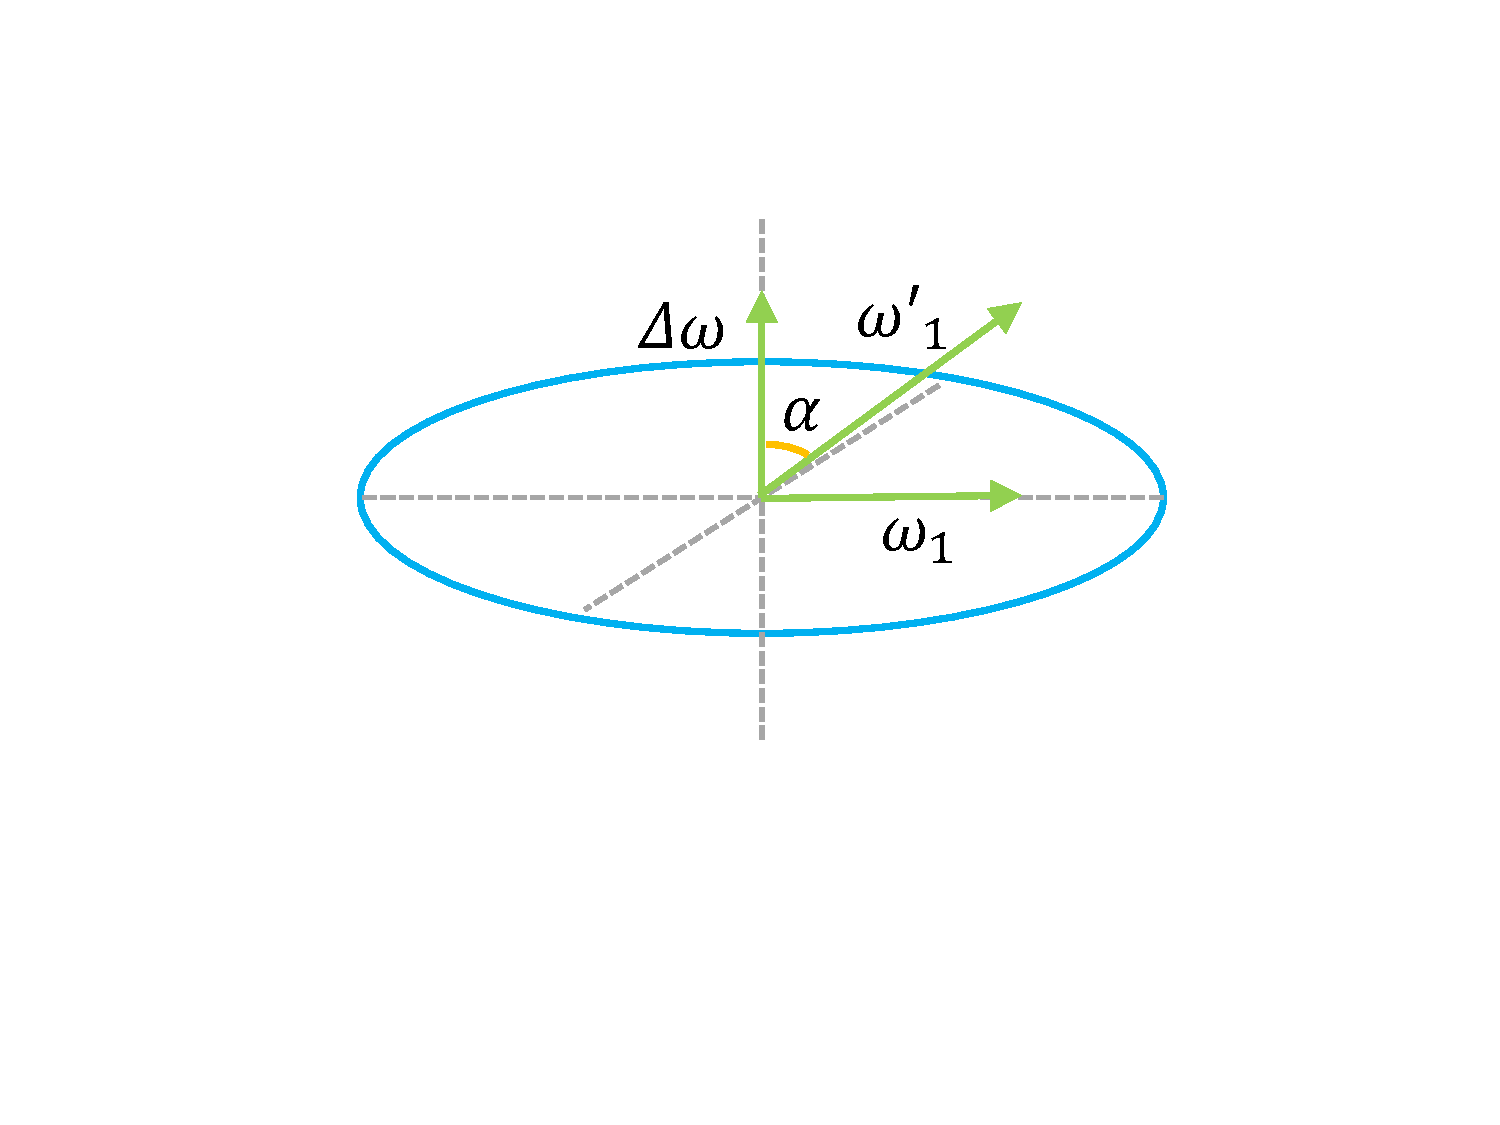
\includegraphics[width= 0.8\columnwidth]{figures/rotate.pdf}
              \caption{偏共振情况下,旋转坐标系中的旋转轴的变化示意图。
              }
              \label{rotate}
            \end{center}
\end{figure}

可以看出,当射频场远离自旋共振频率时,射频场对这个自旋几乎是没有影响的,因为当$|\Delta\omega\gg \omega_1|$时$\alpha$非常小。也就是说,当所有自旋都有分离的很好的Larmor频率的话,原则上我们可以选择性地旋转其中一个,同时对其他自旋没有任何操作。

和上面的旋转频率为$\omega_{rf}$不同,我们也可以选择频率为$\omega_0$的旋转坐标系,那么
\begin{equation}\label{aaa}
H^{rot} = -\hbar\omega_1(cos[(\omega_{rf}-\omega_0)t+\phi]I_x-sin[(\omega_{rf}-\omega_0)t+\phi]I_y).
\end{equation}
除非$\omega_{rf}=\omega_0$,这个变化并不能给出简洁的不含时射频哈密顿量。但对于不同的分离核自旋来说,该形式可以
针对不同的核自旋很好的给出旋转坐标系的形式
\begin{equation}\label{aaa}
\left\vert  \psi \right\rangle^{rot} =[\prod_i e^{-i\omega_0^itI_z^i}]\left\vert  \psi \right\rangle.
\end{equation}

如果是多旋转坐标系的话,射频场的哈密顿量可以类似给出
\begin{equation}\label{aaa}
H^{rot} = \sum_{i,r} -\hbar\omega_1^r(cos[(\omega_{rf}^r-\omega_0^i)t+\phi^r]I_x^i-sin[(\omega_{rf}^r-\omega_0^i)t+\phi^r]I_y^i),
\end{equation}
其中强度$\omega_1^r$和相位$\phi^r$依然是可控的。

在上式的射频场作用下,系统哈密顿量中的单量子项$I_z^i$将由于旋转坐标系的选取而被消掉,而余下的耦合项$J_{ij}I_z^iI_z^j$并不会演化,所以在多旋转坐标系中,
NMR体系的哈密顿量可以表示为
\begin{equation}\label{aaa}
H = H_{sys}+H_{control},
\end{equation}
其中内部哈密顿量为
\begin{equation}\label{aaa}
H_{sys} =  \hbar\sum_{i<j} 2\pi J_{ij}I_z^iI_z^j,
\end{equation}
而外部哈密顿量为
\begin{equation}\label{aaa}
H_{control} =  \sum_{i,r} -\hbar\omega_1^r(cos[(\omega_{rf}^r-\omega_0^i)t+\phi^r]I_x^i-sin[(\omega_{rf}^r-\omega_0^i)t+\phi^r]I_y^i).
\end{equation}

\subsection{弛豫和退相干机制}

利用核自旋作为qubit的一个优点就是NMR系统和周围的环境有很好的隔离,使得其退相干时间相比于动力学演化的时间可以很长。我们这里的讨论仅局限于
封闭系统的动力学演化,当然很多时候这个近似有一定的限制性。

NMR系统与环境的相互作用可以通过一个外加的哈密顿量$H_{env}$来描述。相比于$H_{sys}$ 或$H_{control}$来说它的作用比较小。量子信息的丢失,也就是退相干,正是源于该相互作用机制,一般又由
两个比例来描述:退极化过程(depolarizing)$T_1$ 以及退相位(dephasing)过程 $T_2$。

$T_1$是由自旋-晶格相互作用引起的,或者说在Larmor频率尺度上损失能量子的激发模式产生的,比如振动量子,顺磁离子,同溶剂间
存在离子交换的化学反应,或者有高阶磁矩的自旋等。在选择的比较好的分子及溶剂中,$T_1$的尺度大概为数十秒。NMR中的$T_1$机制类似于
其他物理系统中的非弹性散射,它会带来能量的损失。

$T_2$主要源于系统哈密顿量中没有被完全平均掉的自旋-自旋耦合。比如,在液体NMR分子中,一个分子内的自旋可能和
其他分子中的自旋有很弱的长程相互作用。其他的一些机制,例如化学位移的空间各向异性,顺磁离子等也对$T_2$的大小有一定的贡献。
尽管如此,在好的样品以及高磁场的NMR谱仪中,溶剂分子中的$T_2$可以轻易达到秒量级。$T_2$机制类似于其他物理系统中的弹性散射,系统并不会有任何的能量损失。

对于弛豫机制仅用两个参数来描述其实是对真实物理系统的过度简化,特别在耦合的自旋系统中,还有耦合弛豫机制在产生作用\cite{relax1,relax2}。尽管如此,独立的自旋
退相干模型依然非常有用,它可以很好的抓住主要效应,因为NMR量子计算中的脉冲序列时间基本都是短于$T_2$的。

\section{NMR中的脉冲技术}

前面已经提到,任何幺正操作都可以拆解为任意角度的单比特旋转门和两比特受控门,比如CNOT门的组合。
换句话说,如果要证明NMR量子计算是普适的,我们只需要能够有效实现任意角度的单比特旋转和CNOT门就可以了。在本节中,
我们将介绍如何利用NMR脉冲技术实现量子计算所需的逻辑操作。

\subsection{基本脉冲技术及单量子比特门的实现}

对于一个作用时间为$t_{pw}$的射频脉冲来说,如果它的强度为$\omega_1$且$\omega_{rf}=\omega_0$,那么
其作用的自旋感受到的幺正操作为
\begin{equation}\label{aaa}
U =exp[i\omega_1 (cos \phi I_x- sin \phi I_y)t_{pw}].
\end{equation}
该操作$U$描述的是Bloch球上在$\hat{x}-\hat{y}$平面内绕相位为$\phi$的轴转$\theta$角
\begin{equation}\label{aaa}
\theta =\omega_1 t_{pw}.
\end{equation}
那么,对一个精心设计过时间和相位的脉冲来说,它可以实现绕$\hat{x}$轴的$\pi /2$旋转,简记为$R_x(\pi/2)$或者$X$。如果把脉冲时间加倍,就可以实现$R_x(\pi)$,简记为$X^2$。通过改变射频脉冲
的相位,我们也可以执行$Y$和$Y^2$旋转。

原则上$\hat{x}$和$\hat{y}$方向的任意角度旋转可以实现所有的单比特任意角度旋转。比如要实现$Z$我们有两种基本的$X$和$Y$的组合脉冲可以利用
\begin{equation}\label{aaa}
Z = XY\overline{X} = Y\overline{X}\overline{Y}.
\end{equation}
要注意的一点是这里的操作是从右往左加的,并且对于以后出现的任何复合幺正操作都是如此。

我们可以通过施加一个足够长的软脉冲(soft pulse)选择性地激发一个自旋,同时不影响到分子中的其他自旋。这种软脉冲,或者叫形状脉冲(shape pulse)首先要把中心频率设置在要激发的自旋共振频率上,只影响一定频率范围内的核自旋(显然这个频率范围内不能覆盖其他的核自旋)。它从一个很低的强度$B_1$开始,逐渐加大到最大强度,再逐渐降低直至脉冲末尾。
一般来说,形状脉冲要分为几十甚至几百小片,通过改变每一小片的强度和相位,组合得到整个脉冲的强度和相位大小。对于脉冲宽度为$t_{pw}$的形状脉冲来说,傅里叶变换大概告诉我们它的频率范围为
$1/t_{pw}$。当然,这只是一个大致的结果,因为傅里叶变换是线性变化而射频场的变化是正弦型的,要得到精确的频率覆盖范围要用到其他的计算方法。

\begin{figure}[htbp]
            \begin{center}
              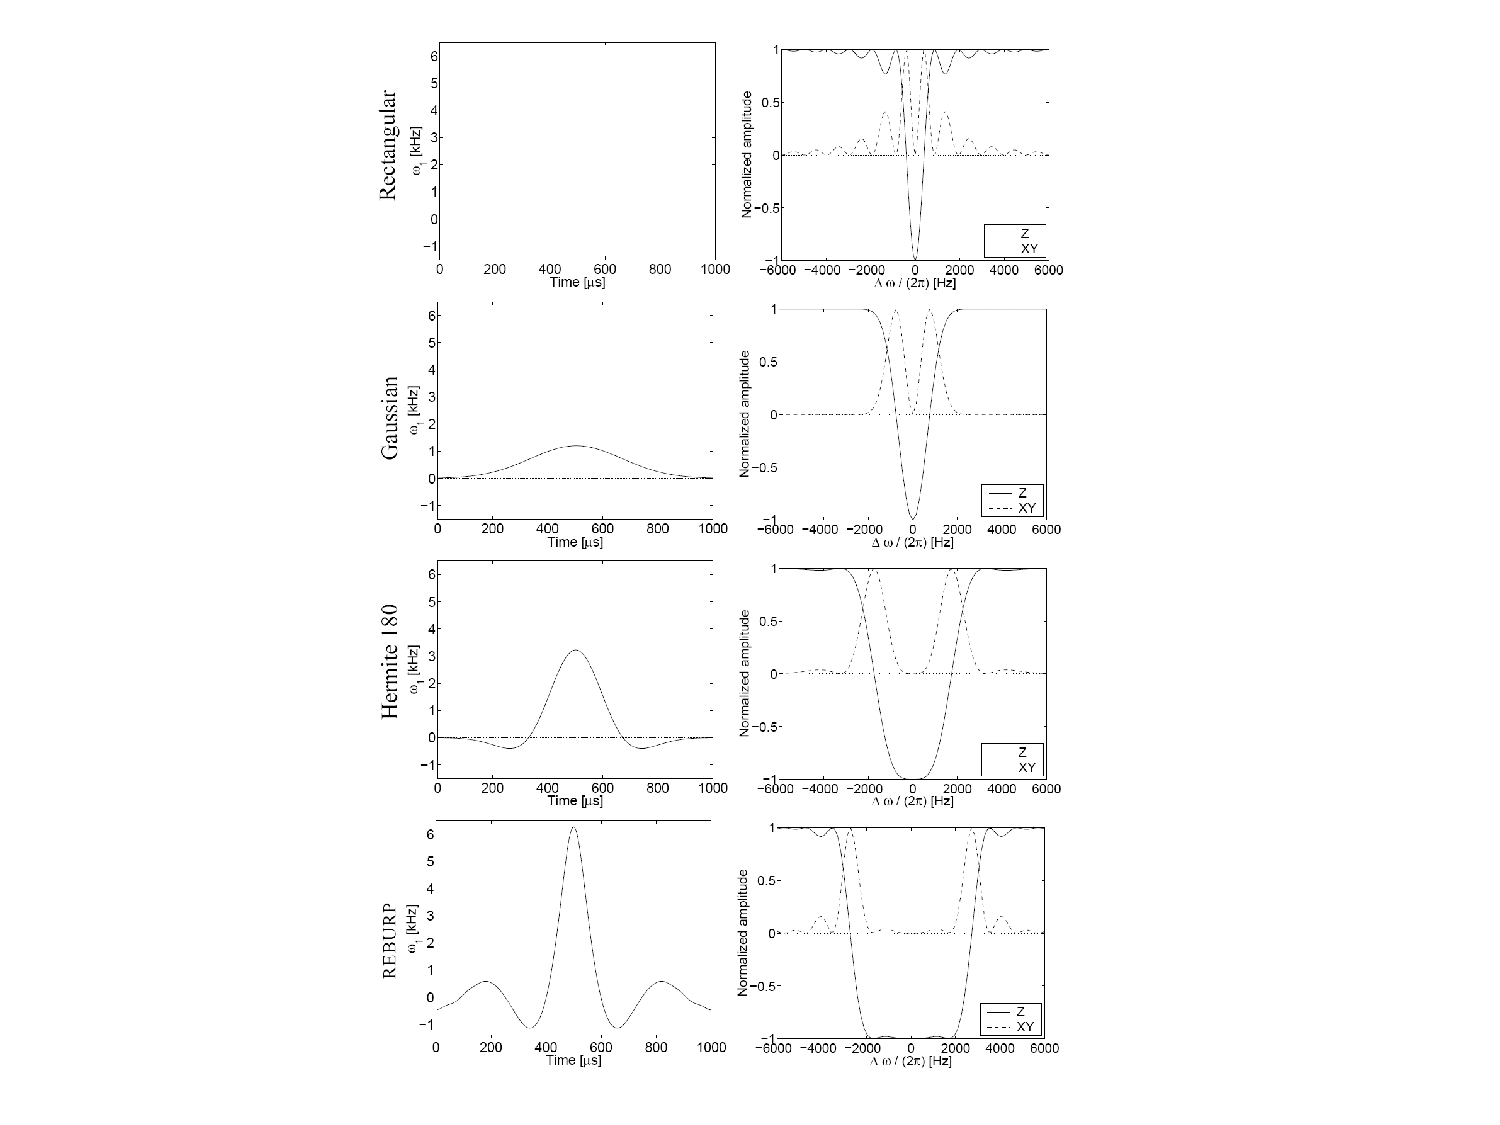
\includegraphics[width= 0.8\columnwidth]{figures/shape.pdf}
              \caption{常用的形状脉冲之间的脉冲宽度(左)与激发频率(右)比较。
              }
              \label{shape}
            \end{center}
\end{figure}

衡量形状脉冲的参数和指标很多,包括:

$\bullet$ 选择性:激发带宽与脉冲宽度的乘积,这个值越低说明选择的效果更好。这点很好理解,比如同样要选1000Hz的频率范围,如果形状脉冲A只用1$ms$就可以做到,而B需要10$ms$,显然A的选择性要比B好。

$\bullet$ 跃迁范围:除了需要的激发频率外,形状脉冲会影响到其他频率区域,这些区域就是跃迁范围。当然这个值越小越好。

$\bullet$ 脉冲强度:对于给定的脉宽,形状脉冲要求的峰值强度。这个值越低则该形状脉冲的要求越低。

 $\bullet$
 自回聚能力:能够回聚掉选择自旋与其他自旋间的$J$耦合的能力。这个值越大说明脉冲效果越好。

  $\bullet$
  鲁棒性:对于实验不完美性,比如射频场不均匀性等各种误差的灵敏度。这个值越大说明形状脉冲的抗噪声能力越强。

$\bullet$
普适性:形状脉冲是不是对任意的输入态或者只对特定输入态可以执行完美的旋转操作。

下表总结了常用的形状脉冲的特点\cite{shape1,shape2,shape3,shape4}。这些脉冲都是普适的,因为一般用于量子计算的态是任意态。明显可以看出,没有哪一个形状脉冲是所有
参数都是最优的,具体的脉冲选择要根据实验需求来定。比如,当化学位移的差别很大时,就没有必要要很小的
跃迁范围。

\begin{figure}[htbp]
            \begin{center}
              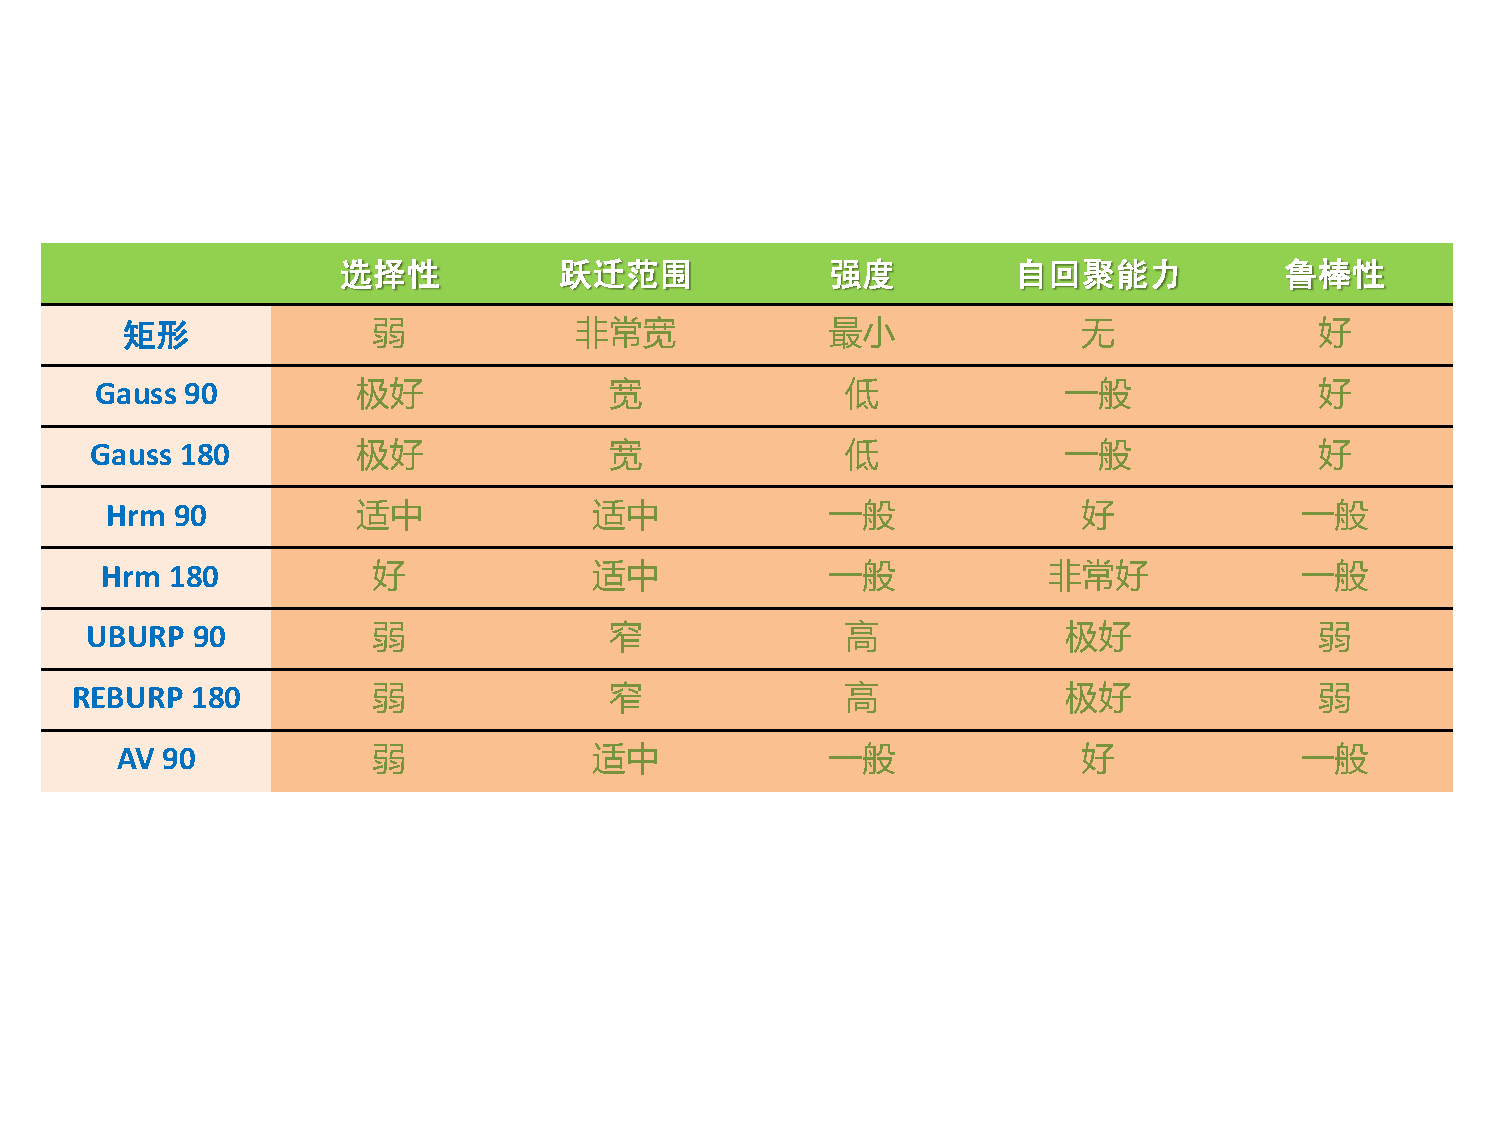
\includegraphics[width= 0.8\columnwidth]{figures/shapepara.pdf}
              \caption{各种形状脉冲之间的比较。
              }
              \label{shapepara}
            \end{center}
\end{figure}

对于异核分子来说,由于各个核之间的Larmor频率相差很大,所以激发不同核的脉冲几乎不需要选择性,所以其脉宽可以很短,比如10$\mu s$。这种脉冲的覆盖范围很大,一般可以覆盖所有同种原子核的频率。由于其强度相对于软脉冲非常大,所以叫做硬脉冲(hard pulse)。当然对于同核分子,比如$^{13}$C标记的Alanine中的三个$^{13}$C,要激发其中一个自旋的话我们不能用硬脉冲而只能选择软脉冲,或者后面将提到的更优秀的
GRAPE脉冲。

\subsection{脉冲重聚及两量子比特门的实现}

如果要实现CNOT门,最常见的方法是利用自旋间的耦合哈密顿量演化。从NMR的系统哈密顿量形式中,我们可以得到时间演化算子
\begin{equation}\label{aaa}
U_J(t) = e^{-i2\pi JI_z^1I_z^2t},
\end{equation}
或者其矩阵形式
\begin{equation}\label{aaa}
U_J(t) = \left(
           \begin{array}{cccc}
             e^{-i\pi J t/2} & 0 & 0 & 0 \\
             0 & e^{i\pi J t/2} & 0 & 0 \\
            0 & 0 & e^{i\pi J t/2} & 0 \\
             0 & 0 & 0 & e^{-i\pi J t/2} \\
           \end{array}
         \right).
\end{equation}
如果选择演化时间为$t = 1/2J$并在各个比特上加一个$\pi/2$的相移,我们将得到一个控制相位门(忽略掉全局相位)
\begin{equation}\label{aaa}
U_{CPHASE} = \sqrt{-i}\overline{Z_1}\overline{Z_2}U_J(1/2J)=\left(
           \begin{array}{cccc}
             1 & 0 & 0 & 0 \\
             0 & 1 & 0 & 0 \\
            0 & 0 & 1 & 0 \\
             0 & 0 & 0 & -1 \\
           \end{array}
         \right).
\end{equation}
CPHASE门的形式和CNOT门已经非常接近,控制比特上只差一个相位,而目标比特上只差简单的单比特旋转,
\begin{equation}\label{ucnot}
U_{CNOT} = iZ_1^2\overline{Y_2}U_{CPHASE}Y_2 = \sqrt{i}Z_1\overline{Z_2}X_2U_J(1/2J)Y_2=\left(
           \begin{array}{cccc}
             1 & 0 & 0 & 0 \\
             0 & 1 & 0 & 0 \\
            0 & 0 & 0 & 1 \\
             0 & 0 & 1 & 0 \\
           \end{array}
         \right).
\end{equation}
执行$U_{CNOT}$序列的核心是$X_2U_J(1/2J)Y_2$,其作用可以通过图\ref{nmrcnot}形象说明:假设两个自旋都处于$\pm \hat{z}$。首先自旋2绕$\hat{y}$旋转$\pi/2$,到达$\hat{x}$轴。然后整个系统在相互作用哈密顿量下自由演化$1/2J$的时间。由于自旋2的进动频率
依赖于自旋1所处的状态$\left\vert  1 \right\rangle$或者$\left\vert  0 \right\rangle$而会移动$\pm J/2$,自旋2在自由演化后所处的状态也会依赖于自旋1所处的状态而处于$+\hat{y}$或$-\hat{y}$轴。最后,自旋2绕$\hat{x}$旋转$\pi/2$。如果自旋1处于$\left\vert  0 \right\rangle$,自旋2将回到$+\hat{z}$;如果自旋1处于$\left\vert 1 \right\rangle$,自旋2将回到$-\hat{z}$。整体来看,当且仅当自旋1处于$\left\vert 1 \right\rangle$时,自旋2进行了翻转,而式\ref{ucnot}中的$\hat{z}$旋转则可以把所有的矩阵元调整到和$U_{CNOT}$完全一样。

\begin{figure}[htbp]
            \begin{center}
              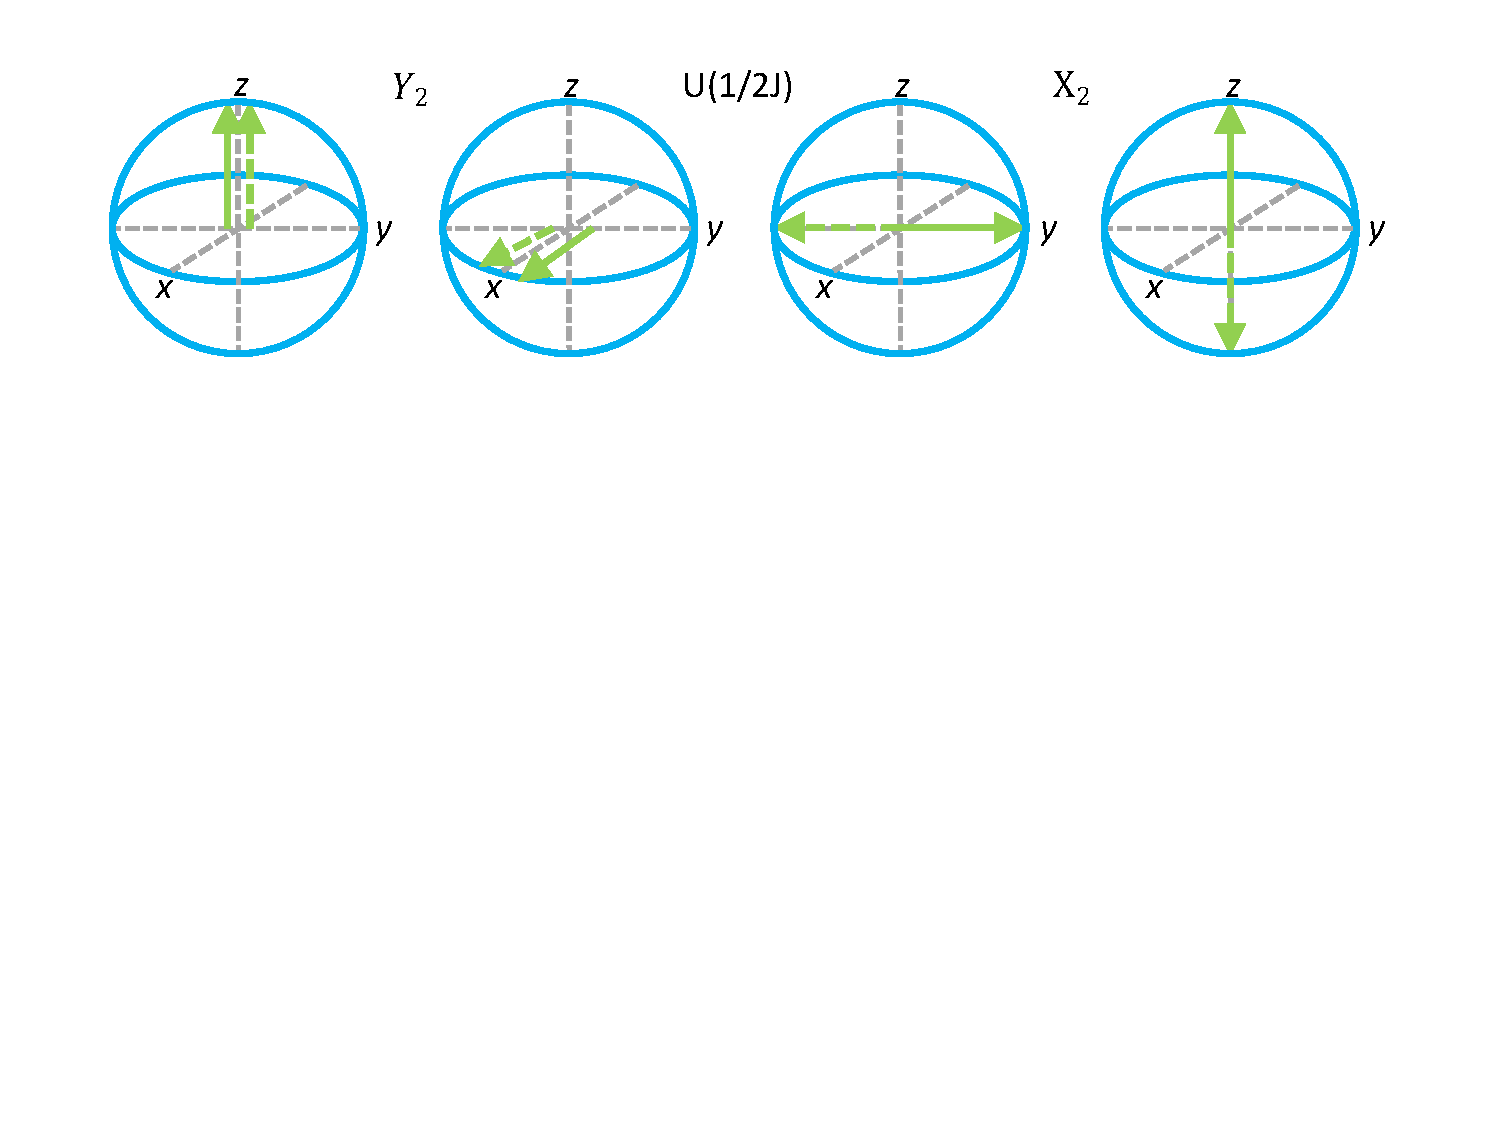
\includegraphics[width= 0.8\columnwidth]{figures/nmrcnot.pdf}
              \caption{CNOT门的Bloch球表示。目标比特2刚开始处于$\left\vert  0 \right\rangle$态,实线和虚线分别表示控制比特1处于$\left\vert  0 \right\rangle$和$\left\vert  1 \right\rangle$时qubit 2所处的状态。
              }
              \label{nmrcnot}
            \end{center}
\end{figure}

另外一种实现CNOT门的方法是利用线选脉冲。如果对处于频率$\omega_0^2+J/2$的峰施加一个选择性的$\pi$脉冲,它的作用是当且仅当控制比特1处于$\left\vert  1\right\rangle$时目标比特2将被翻转。当一个自旋和更多的自旋有耦合作用时,为了实现CNOT我们需要同时选择性地激发该自旋的一半的峰。目前实验上已经在五个qubit的系统上利用非常长的多频率激发脉冲 实现了CNOT门\cite{linecnot}。但当一个自旋的峰并没有分的很开时这种方法非常难以适用。

如果自旋间的相互作用哈密顿量不是$I_z^iI_z^j$的形式,还包括其他的横向分量,我们可以利用其他的脉冲序列
执行CPHASE和CNOT门,不过这些序列会很复杂\cite{linecnot2}。

如果两个自旋间并没有直接的相互作用,我们依然可以实现CNOT门,只要这两个自旋可以通过一系列的耦合连接起来。反过来,如果
一个自旋和很多的自旋间有相互作用,我们想执行它和另一个自旋间的CNOT的话则必须移除其他耦合的影响。一般来说,在NMR量子计算中常用的是已经在很多NMR实验中广泛运用的脉冲重聚技术。

在液体NMR中,耦合哈密顿量形式一般为$I_z^iI_z^j$,针对这种哈密顿量的重聚比较容易理解。如果耦合哈密顿量还包含横向分量的话,重聚过程就比较复杂了,需要运用平均哈密顿量的
理论来解释。

首先我们来看看如何在两qubit系统中消除$I_z^iI_z^j$形式的耦合。从数学形式来看,对于任意的演化时间$\tau$,总有
\begin{equation}\label{aaa}
X_1^2U_J(\tau)X_1^2 =U_J(-\tau) =X_2^2U_J(\tau)X_2^2,
\end{equation}
也就是
\begin{equation}\label{aaa}
X_1^2U_J(\tau)X_1^2U_J(\tau) =I=X_2^2U_J(\tau)X_2^2U_J(\tau).
\end{equation}
在上式中把所有的$X_i^2$替换为 $Y_i^2$,序列依然是类似的。如果有时用$X_i^2$,有时用 $Y_i^2$,我们得到的单位矩阵将有一些相位差别,但是如果同时在两个qubit上都加$\pi$脉冲的话,即
$X_1^2X_2^2U_J(\tau)X_1^2X_2^2U_J(\tau) $,耦合是不会被回聚的。

\begin{figure}[htbp]
            \begin{center}
              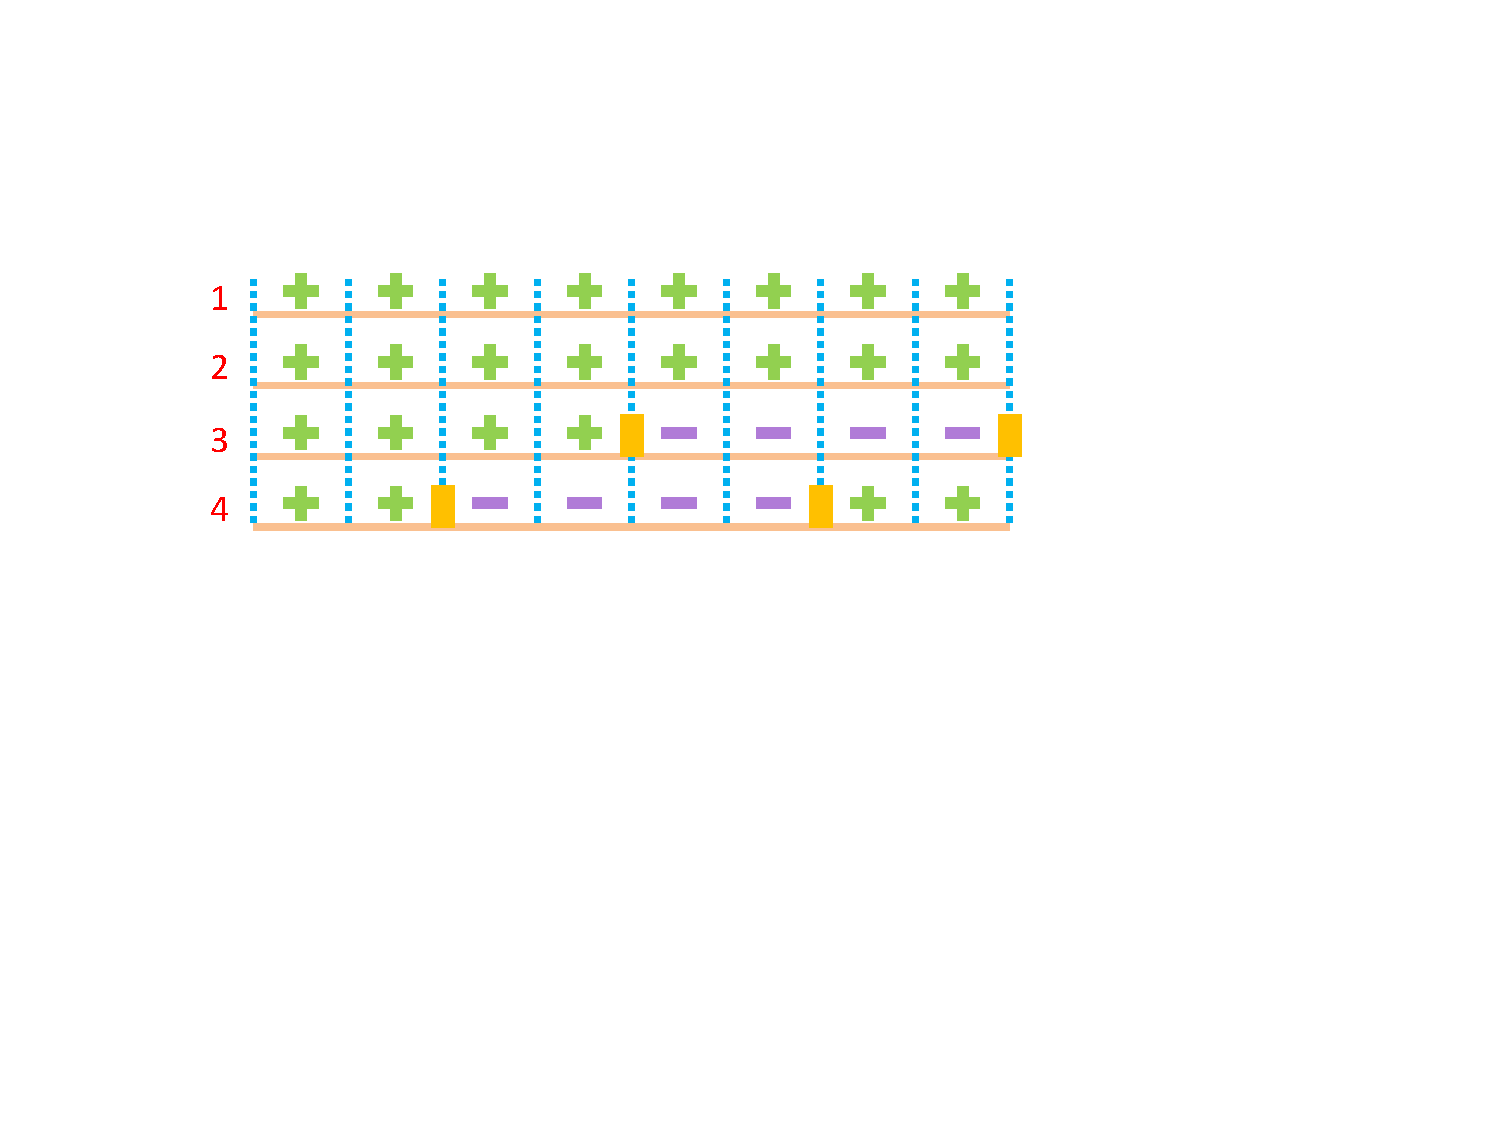
\includegraphics[width= 0.8\columnwidth]{figures/refocusing.pdf}
              \caption{四比特系统中只保留$J_{12}$形式的耦合的脉冲重聚序列。每一小段所代表的演化时间是相同的,黄色的矩形代表$\pi$脉冲,用来翻转当前自旋的状态。
              }
              \label{refocusing}
            \end{center}
\end{figure}

图\ref{refocusing}给出了多比特系统中的重聚技术。该序列有效地保留了$J_{12}$的效果,同时消除了其他耦合的影响。当一段耦合之内的自旋$i$和$j$处于相同的符号时,
可以认为耦合演化表现出来的效果是正方向的,而当两个自旋处于相反的符号时,耦合演化表现出来的效果是负方向的。只要一个耦合总体表现出来的正方向和负方向的时间是相同的,那么它的效果将
被回聚掉,没有任何影响。

在NMR量子计算中,设计重聚序列的系统化方法也已经发展起来。最常用的方案是基于Hadamard矩阵\cite{refo1,refo2}。
$n\times n$的Hadamard矩阵$H(n)$满足
\begin{equation}\label{aaa}
H(n)H(n)^T = nI.
\end{equation}
$H(n)$中所有行都是两两正交的,比如$H(12)$的例子如下图\ref{hadamard}

\begin{figure}[htbp]
            \begin{center}
              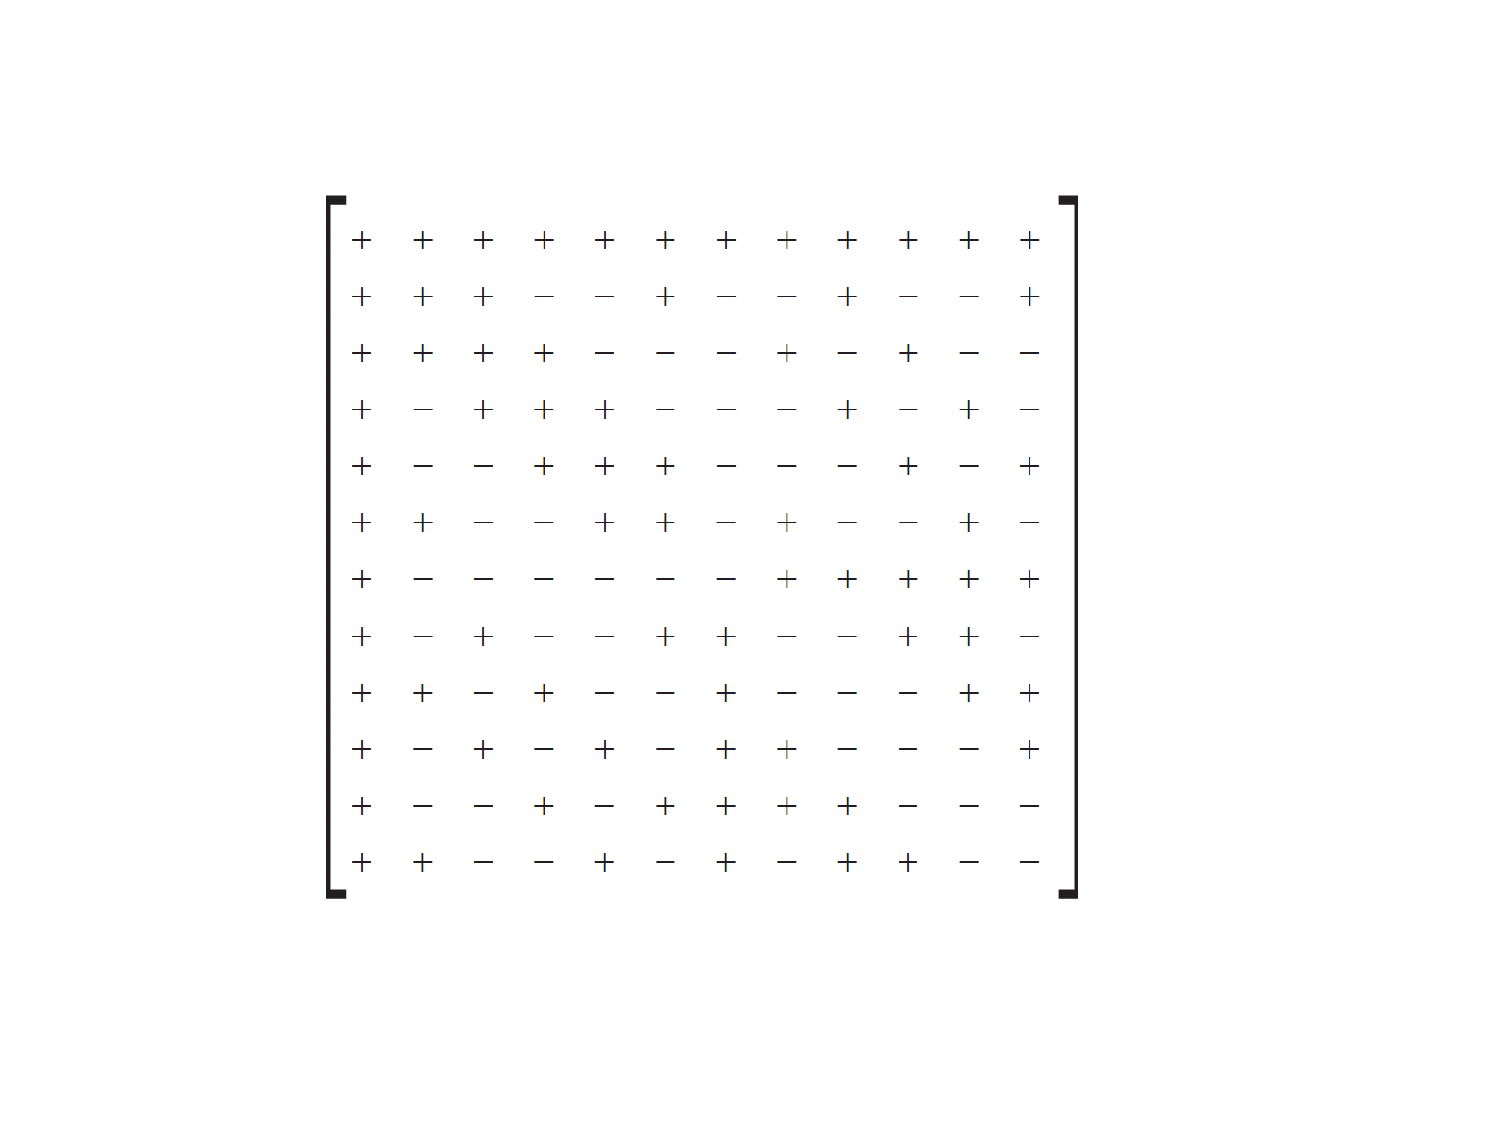
\includegraphics[width= 0.8\columnwidth]{figures/hadamard.pdf}
              \caption{重聚序列$H(12)$的形式。
              }
              \label{hadamard}
            \end{center}
\end{figure}

如果我们想保留任意一对耦合,同时回聚掉其他耦合的话,只需要简单的对$H(n)$中的那两个qubit用相同的行形式就可以了。

$H(n)$并不是对所有$n$都是存在的,但我们总可以找到一个$\overline{n}$,使得$H(\overline{n})$是已知的,且$\overline{n}\geq n$。因此对于$n$个自旋的系统我们需要$\overline{n}$个时间间隔来实现重聚,且$\pi$脉冲的个数不多于$n\overline{n}$个。

另外一种设计重聚序列的系统方法是Linden等人提出的\cite{refo3}。在四比特系统中,该序列形式如下
\begin{equation}\label{aaa}
\left(
  \begin{array}{cccccccc}
    + & + & + & + & +& +& + &+ \\
    + & + & + & + & - & - & - & - \\
    + & + & - & - & - & - & + & + \\
    + & - & - & + & + & - & - & + \\
  \end{array}
\right).
\end{equation}
每附加一个qubit,演化时间间隔的数量就翻倍,并且$\pi$脉冲在这个qubit上施加在第一,第三,第五个......时间间隔之后。同基于
Hadamard矩阵的方案相比,该方案不要求同时对多个qubit进行旋转,但该方案的时间间隔数目随着qubit的增加而指数增长。

%\subsection{梯度场技术}

%现代的NMR谱仪都配有在任意方向施加梯度磁场的线圈。假设梯度场的方向为$\hat{z}$方向,那么整个磁场的形式将是
%\begin{equation}\label{aaa}
%B(z) = B_0 + \gamma z B_1,
%\end{equation}
%其中$B_0$和$B_1$分别是静磁场和梯度场的强度。

\subsection{强调制脉冲及GRAPE脉冲技术}

在本章的第一节我们已经说过,对于同核系统来说,为了选择性地激发其中一个核自旋我们需要形状脉冲,但形状脉冲的缺点非常多。例如,它的强度比较低,也就意味着其作用时间很长,会带来
不可忽略的退相干效应,同时其作用时间内的内部哈密顿量演化也必须考虑。如果对一个NMR系统施加过多的形状脉冲,实验结果的误差将会是非常大的,量子计算的任务也不会有效的完成。

为了克服形状脉冲带来的低精度问题,2002年MIT的Cory小组提出了强调制脉冲(Strongly modulating pulses, SMP)\cite{smp1}理论,通过计算机的搜索和优化来强调制形状脉冲中的各个参数,从而精确实现所需的逻辑操作。由于SMP的脉冲能量一般很高,所以系统弛豫的影响将大大减小,同时优化过程中还能补偿一些系统误差的影响,例如射频场的不均匀性。
2005年,Glaser小组则利用梯度上升算法(gradient ascent pulse engineering, GRAPE)来设计形状脉冲,使得其效率和精度进一步提高。在本节中我们将简要介绍这两种在当前NMR量子计算领域极其重要的脉冲设计理论。

(a) \emph{强调制脉冲技术}

给出一个形状脉冲,我们可以轻松的计算出其演化算子,但反过来则非常困难。借助一些传统的分析技术,例如平均哈密顿量理论我们可以分析出合适的控制脉冲形式,但借助现代计算机及数学上的算法我们可以更有效且精确地给出
问题的解。从传统意义上说,强调制脉冲(Strongly modulating pulses, SMP)\cite{smp1,smp2,smp3}非常类似于形状脉冲。SMP中包含的脉冲数目并不算多,但是它们的强度,频率,脉宽以及相位都可以不同。强调制过程可以
理解为一种确定形状脉冲中各个参数的方法,其利用的多是数值模拟而非解析计算。 发展SMP技术的初衷是希望能够有效实现复杂的多自旋系统中的量子逻辑操作。在传统的方法中,例如利用自旋回波重聚技术来孤立哈密顿量中需要的项,然后构造逻辑网络图的方法在大的自旋体系中非常难以扩展。
上一小节中我们已经看到脉冲重聚随着比特数及相互作用数目增加时会变得非常复杂,而SMP的思路是通过不断改变和优化射频场的参数,并把所有的小片脉冲级联起来,使得整个脉冲的效果可以很好的实现需要的演化算子。
同时,在SMP中,很多系统误差,例如射频场的不均匀性等都可以考虑到优化过程中,使得最后搜索出来的SMP可以抗干扰。下面我们将给出SMP的设计方法。

首先,我们要确定如何衡量搜索得到的SMP所代表的幺正算子$U_{SMP}$和理论要求的幺正算子$U_{tar}$之间的相似程度,一般我们采用量子门保真度(quantum gate fidelity)的概念
\begin{equation}\label{aaa}
F = |\textbf{Tr}(U_{tar}^{\dagger}U_{SMP})/N|^2,
\end{equation}
其中$N=2^n$是Hilbert空间的维度。$F$越大,说明搜索到的SMP越好。关于保真度的具体讨论详见下一小节。

通过$F$,我们定义一个$Q$因子,
\begin{equation}\label{aaa}
Q = 1-\sqrt{F}.
\end{equation}
Q越小,也说明搜索到的SMP效果越好。在具体的程序中,我们就是用$Q$因子的大小作为衡量SMP的搜索结果的标准。

回忆本章刚开始时所讲过的,NMR系统的内部哈密顿量为
\begin{equation}\label{aaa}
H_{int} =-\hbar\sum_{i}\omega_0^i I_z^i+ \hbar\sum_{i<j} 2\pi J_{ij}I_z^iI_z^j.
\end{equation}
而外部哈密顿量也就是射频场的形式为
而外部哈密顿量为
\begin{equation}\label{aaa}
H_{ext} =  -\hbar\omega_1(cos[(\omega_{rf}-\omega_0^i)t+\phi]I_x^i-sin[(\omega_{rf}-\omega_0^i)t+\phi]I_y^i).
\end{equation}
从射频场的形式我们可以看出,射频场一共存在四个可变参数:能量$\omega_1$,频率$\omega_{rf}$,周期$t$和相位$\phi$。
那么演化算子
\begin{equation}\label{aaa}
U = e^{-i(H_{int}+H_{ext})t}.
\end{equation}
通过Nelder-Mead算法\cite{smp4},我们在整个空间内搜索这四个参数,使得$Q$因子尽可能的小。如果此时搜索得到的$U_{SMP}$和理论值$U_{tar}$之间非常接近,也就是$Q$很小,那么我们就保留这个结果并作为NMR实验上用的SMP。
但一般来说对于多自旋体系,单个的射频脉冲很难精确到获得所需操作,我们一般选择多个射频脉冲级联的方式,并且把每一小片脉冲中的
能量$\omega_1$定为常数,则有
\begin{equation}\label{aaa}
U_{net} = \prod_{m=1}^N U_m = \prod_{m=1}^N e^{-i(H_{int}+H_{ext}^m(\omega_1, \omega_{rf}^m, \phi^m, t^m))t^m}.
\end{equation}
序号$m$指的就是第$m$个方形脉冲小片。如果依然达不到所需结果,那么方形脉冲的数目还会继续增加。
%下面给出两个SMP的例子,分别是在3-qubit Alanine样品中的$R_x^3(\pi/2)$操作和4-qubit Crotonic中的 $R_x^{1,2}(\pi)$操作。

要注意的是,NMR实验并不会和理论计算的结果完全一样。在同一个样品中,处于不同位置的不同核自旋感受到的外磁场并不会完全一样,而且这些核自旋的化学位移也会
有轻微的差别。定义处于$\overrightarrow{r}$的自旋感受到的幺正操作为$U(\overrightarrow{r})$的话,整个NMR样品的密度矩阵演化过程大致可以写成一个非幺正的过程
\begin{equation}\label{aaa}
\rho(t) = \int U(\overrightarrow{r})\rho(0)U^{\dagger}(\overrightarrow{r})d\overrightarrow{r}),
\end{equation}
将化学位移和射频场的权重因子代入,则有
\begin{equation}\label{aaa}
\rho(t) = \int p(\omega,\Omega)U(\omega,\Omega)\rho(0)U^{\dagger}(\omega,\Omega)d\omega d\Omega).
\end{equation}
其中$\omega$是射频场的能量,而$\Omega$是化学位移。这是一个超算子的求和形式,其保迹条件为
\begin{equation}\label{aaa}
\int p(\omega,\Omega)d\omega d\Omega) =1.
\end{equation}

由于在实验中化学位移的变化对SMP的保真度影响并不大,我们着重考虑射频场不均匀性带来的影响。不均匀性的分布权重$p(\omega)$在实验上可以用
文献中的方法测出\cite{smp5},然后用新的含射频场分布权重因子的能量代替以前的射频能量
\begin{equation}\label{aaa}
\omega = \sum_{i = 1}^np(\omega_i)\omega_i,
\end{equation}
$n$为补偿不均匀性的取点个数,其值越大,修正就越好,但也会大大增加计算的复杂度。我们在实验上一般取3到5个点。

此时含射频场不均匀性的SMP的保真度形式为
\begin{equation}\label{aaa}
F = \sum_i|\textbf{Tr}(\sqrt{p(\omega_i)}U_{tar}^{\dagger}U_{\omega_i})/N|^2.
\end{equation}
至此我们就完成了SMP的射频场不均匀性的修正。

(b) \emph{GRAPE脉冲技术}

在多比特数时,SMP的方法并不是最优化的,而且SMP中每个脉冲小片都是方波,参数的跳变也会给具体的实验带来一定的误差。
德国的Glaser小组则从一个标准的优化控制思想出发,提出了GRAPE算法\cite{smp6}。

一个自旋体系的密度矩阵演化可以用Liouville Von-Neumann方程给出
\begin{equation}\label{aaa}
\dot{\rho}(t) = -i[(H_{int}+\sum_{k=1}^mu_k(t)H_{ext}),\rho(t)].
\end{equation}
$u_k(t)$是能够控制的射频场幅度因子。我们的目标是找到最优的$u_k(t)$,使得经过$T$时间演化后末态$\rho(T)$与理论要求的末态$C$之间尽可能的相似。
为了表征这个相似程度,我们采用两者的内积形式定义为表现因子
\begin{equation}\label{aaa}
\Phi_0 = <C|\rho(T)>.
\end{equation}

\begin{figure}[htbp]
            \begin{center}
              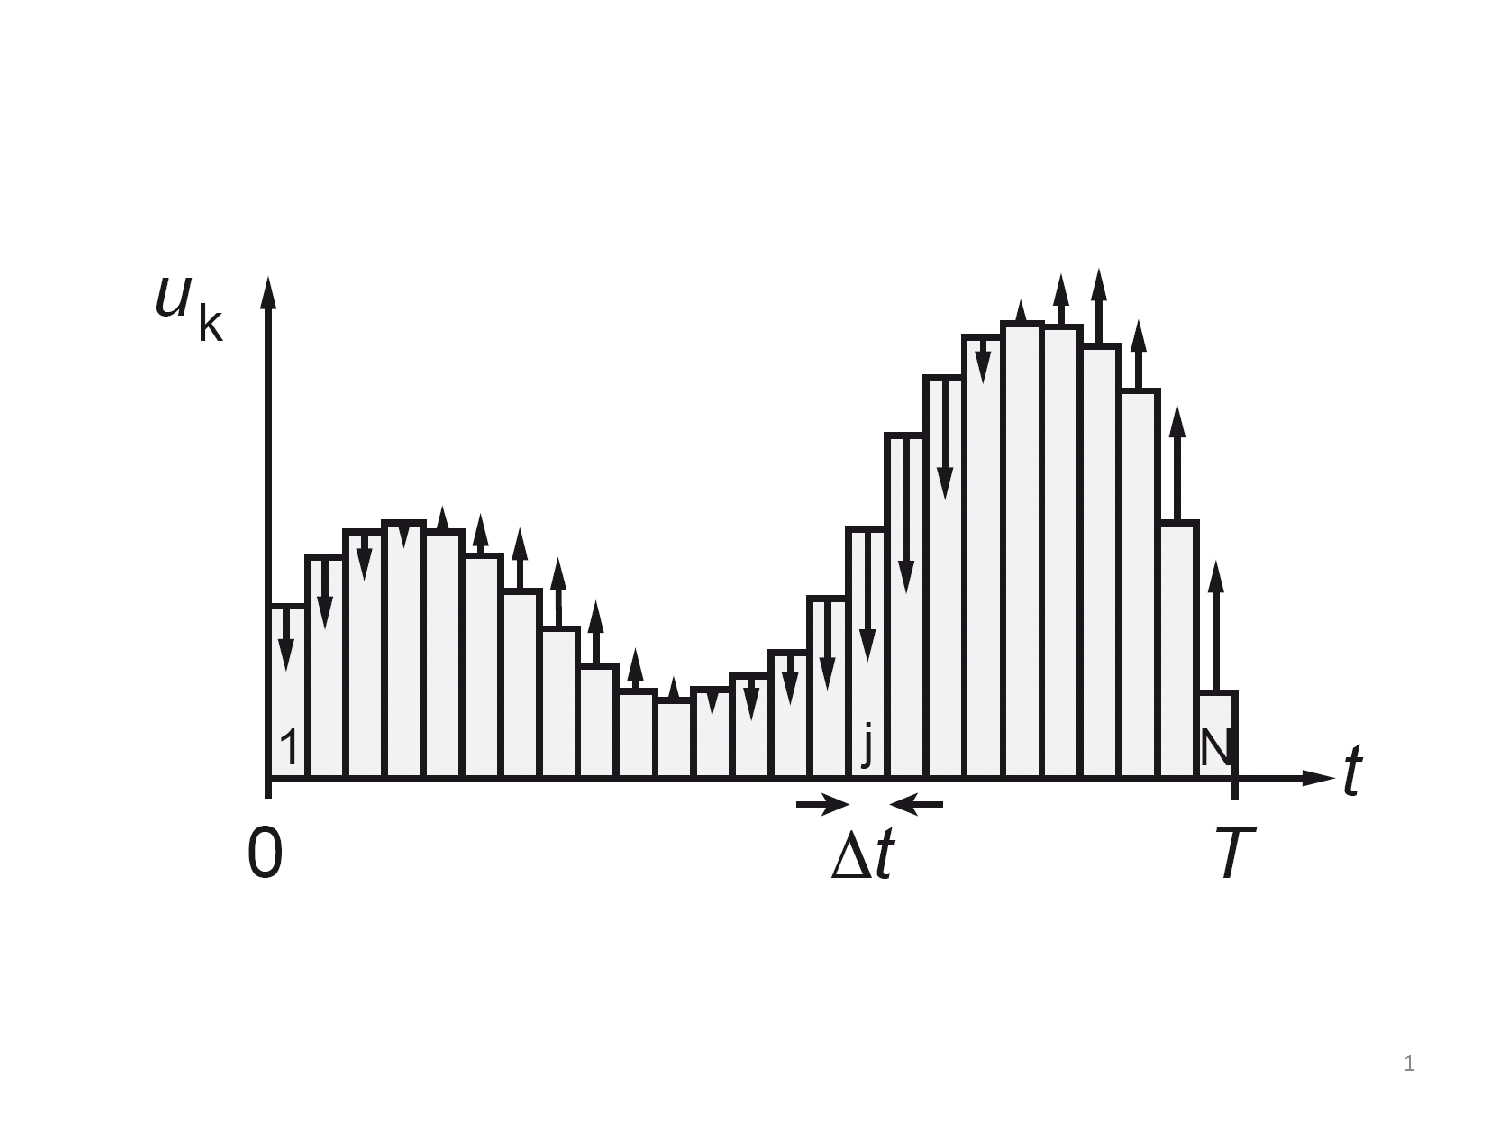
\includegraphics[width= 0.8\columnwidth]{figures/grape.pdf}
              \caption{在GRAPE算法中,每一小步的射频场幅度因子都是常数,而上下箭头表示的是幅度梯度。正是通过计算幅度梯度来改善整个GRAPE脉冲的效果(即$\Phi_0$的值)。
              }
              \label{grape}
            \end{center}
\end{figure}

整个演化时间被分为$N$步,每一步的时间间隔均为$\Delta t = T/N$,并保证每一步中,幅度因子$u_k$都是恒定的(见图\ref{grape})。那么第$j$步的演化算子为
\begin{equation}\label{aaa}
U_j = e^{-i\Delta t ((H_{int} + \sum_{k=1}^mu_k(j)H_{ext})},
\end{equation}
最后的末态密度矩阵为
\begin{equation}\label{aaa}
\rho(T) = U_N\cdots U_1 \rho_0 U_1^{\dagger}\cdots U_N.
\end{equation}
代入表现因子$\Phi_0$的表达式可得
\begin{equation}\label{aaa}
\Phi_0 = <C|U_N\cdots U_1 \rho_0 U_1^{\dagger}\cdots U_N>,
\end{equation}
并改写为
\begin{equation}\label{aaa}
\Phi_0 = <U_{j+1}^{\dagger}\cdots U_N^{\dagger} C U_N\cdots U_{j+1}|U_j\cdots U_1 \rho_0 U_1^{\dagger}\cdots U_j^{\dagger}>.
\end{equation}
后半部分$\rho_j$为$j\Delta t$时刻的密度矩阵,而前半部分$\lambda j$则可以看成是目标态$C$的反演。在某个$j\Delta t$ 时刻,我们通过测量$\Phi_0$的变化来改变$u_k(j)$,达到 $u_k(j)+\delta u_k(j) $。此时整个$U_j$的变化在一阶近似可以写成
\begin{equation}\label{aaa}
\delta U(j) = -i\Delta t \delta u_k(j) \overline{H_k} U(j).
\end{equation}
且
\begin{equation}\label{aaa}
\overline{H_k} \Delta t = \int_0^{\Delta t} U(j)(\tau)H_kU_j(-\tau)d\tau.
\end{equation}
当$\Delta t$趋近于0时,$\overline{H_k} \approx H_k$,即
\begin{equation}\label{aaa}
\frac{\Delta \Phi_0}{\Delta u_k(j)} = -<\lambda_j|i\Delta t[H_k,\rho_j]>.
\end{equation}
当我们采用的变化形式为
\begin{equation}\label{aaa}
u_k(j)\longrightarrow u_k(j) + \epsilon\frac{\Delta \Phi_0}{\Delta u_k(j)}
\end{equation}
时,表现因子$\Phi_0$的值可以被提升,也就是GRAPE的效果会变好。经过一次次的梯度上升,最终我们可以搜索得到精确的GRAPE脉冲。

如果在GRAPE算法中考虑射频场不均匀性的话,我们要采取的修正为
\begin{equation}\label{aaa}
\frac{\Delta \Phi_0}{\Delta u_k(j)} = \sum_i - 2p(\omega_i) Re(<P_j(\omega_i)|i\Delta t H_k X_j(\omega_i)>< X_j(\omega_i)|P_j(\omega_i)>).
\end{equation}

最后要提到的是,无论是计算SMP还是GRAPE脉冲,我们都需要对整个自旋系统进行完整的模拟。就像我们之前一直在提的,对于经典计算机来说
这个模拟过程所需要的资源是随着比特数的增加而指数增长的。其实,最好的设计SMP或GRAPE的方法就是利用一台量子计算机。当然,这有点类似“以子之矛攻子之盾”的含义,
但这确实是在量子计算发展中不可回避的问题,很多研究人员已经尽力在避免使用SMP或GRAPE脉冲了,或者使用精心挑选的
自旋系统来最大限度的规避这些问题。

\section{初态制备及测量读出}

\subsection{NMR中的赝纯态制备方法}

在NMR体系中,自旋初态一般为热平衡态
\begin{equation}\label{aaa}
\rho_{eq} = \frac{e^{-H_0/k_BT}}{\mathcal{Z}} = \frac{1}{\mathcal{Z}}\left(
                                                                       \begin{array}{cc}
                                                                         e^{-\hbar \omega_0/2k_BT} & 0 \\
                                                                         0 & e^{\hbar \omega_0/2k_BT} \\
                                                                       \end{array}
                                                                     \right).
\end{equation}
自旋所处的状态则由Boltzmann分布给出
\begin{equation}\label{aaa}
Pr[\left\vert 0 \right\rangle] = \frac{e^{-\hbar \omega_0/2k_BT}}{\mathcal{Z}} = \frac{e^{-\hbar \omega_0/2k_BT} }{e^{-\hbar \omega_0/2k_BT} +e^{\hbar \omega_0/2k_BT} }
\end{equation}
\begin{equation}\label{aaa}
Pr[\left\vert 1 \right\rangle] = \frac{e^{\hbar \omega_0/2k_BT}}{\mathcal{Z}} = \frac{e^{\hbar \omega_0/2k_BT} }{e^{-\hbar \omega_0/2k_BT} +e^{\hbar \omega_0/2k_BT} }.
\end{equation}
对于典型的NNMR磁场强度,比如10T,$\hbar \omega_0/k_BT\approx 10^{-5} \ll 1$,因此我们可以把指数项进行Taylor展开,得到
\begin{equation}\label{aaa}
\rho_{eq} \approx \frac{1}{2}\left(
                                                                       \begin{array}{cc}
                                                                         1+ \hbar \omega_0/2k_BT & 0 \\
                                                                         0 & 1 - \hbar \omega_0/2k_BT \\
                                                                       \end{array}
                                                                     \right).
\end{equation}
我们把$\varepsilon = \hbar \omega_0/k_BT$定义为自旋的极化度(polarization)。在热平衡态情况下,自旋的极化度几乎为0,自旋处于$\left\vert 0 \right\rangle$的概率$Pr[\left\vert 0 \right\rangle]$与处于$\left\vert 1 \right\rangle$的概率$Pr[\left\vert 1 \right\rangle]$几乎相等。

类似地,对于多自旋体系,热平衡态的形式为
\begin{equation}\label{aaa}
\rho_{eq} \approx \frac{1}{2^n}\left(
                                 \begin{array}{cccc}
                                   1+ \sum_k^n \frac{\hbar \omega_0^k}{2k_BT}  &  &  &  \\
                                    & 1- \frac{\hbar \omega_0^n}{2k_BT} + \sum_k^{n-1}\frac{\hbar \omega_0^k}{2k_BT} &  & \\
                                    &  & \ddots & \\
                                    &  &  & 1- \sum_k^n\frac{\hbar \omega_0^k}{2k_BT} \\
                                 \end{array}
                               \right).
\end{equation}
这里忽略了耦合能量是因为在10T左右的磁场下,$\hbar \omega_0$已经大约是$\hbar2\pi J_{ij}$的$10^6$倍了。

在热平衡态下,我们不可能知道自旋到底处于向上和向下的哪个状态,因为它们处于这些状态的概率几乎完全相等。
这种状态是不适合用作量子计算的初态的,我们需要的是一个单一的,能够确切知道的态(比如$\left\vert 00\ldots 0 \right \rangle$),所以我们必须寻找合适的方法实现NMR的初态制备。

最直观的纯化热平衡态的方法是通过冷却,把初态直接冷却到系统的基态上去。从极化度的表达形式可知,我们要求
热能$k_BT$ 远小于基态与第一激发态的能级差$\hbar \nu$。如果我们能够实现绝对零度,那这个要求自然就满足了。可惜的是这不是电子游戏,并不存在这种强大的冰系招数。对于Larmor频率在1GHz以下的NMR系统来说,这要求温度$T\ll0.05K$!很明显地液体NMR样品是做不到这一点的,因为它们肯定被冻住了。
目前能达到这一温度的NMR样品只有固体样品和液态的$^3$He\cite{pps1}。 以目前的技术手段来看,纯粹通过降温冷却实现NMR量子计算的初态制备是不现实的。

真正实现室温下NMR量子计算依赖于有效纯态(effective pure state)或者叫赝纯态(pseudo-pure state, PPS)的概念的提出。PPS的概念使得室温下进行NMR量子计算成为了可能,这些自旋的动力学行为看上去就和绝对零度时一模一样,至多有一个信号强度的差别。下面我们将解释NMR量子计算中非常重要的PPS的概念,并给出常用的
制备PPS的方法。

制备PPS的出发点首先依据的是NMR中非常重要的一个事实:NMR信号只和布居度之差有关,和布居度本身的大小并无任何关系。也就是说,一个单位矩阵在NMR中是不会产生任何信号的。同时,由于$UIU^{\dagger}=I$,单位阵也不会在
幺正操作下进行任何动力学演化。那么,在NMR中,我们只关心偏移密度矩阵(deviation density matrix)$\rho_{\Delta}$的概念,也就是在整个密度矩阵中减掉毫无用处的单位阵
\begin{equation}\label{aaa}
\rho_{\Delta} = \rho-I/2^n.
\end{equation}
这里我们已经假定$\rho$是归一化的,即$\textbf{Tr}(\rho) = 1$。

Gershenfeld和Chuang\cite{nmrpro2},以及Cory小组\cite{nmrpro1}分别独立发现下面的密度矩阵形式
\begin{equation}\label{aaa}
\rho_{eff} = \frac{1-\alpha}{2^n}I +\alpha \left\vert \psi \right \rangle \left\langle \psi \right \vert
\end{equation}
的动力学性质和它的第二项$\left\vert \psi \right \rangle \left\langle \psi \right \vert$相同,而$\left\vert \psi \right \rangle \left\langle \psi \right \vert$代表了一个纯态。因此我们就叫$\rho_{eff} $ 为有效纯态或赝纯态。

假设$\left\vert \psi \right \rangle = \left\vert 00\ldots 0 \right \rangle$的话,可以写出
 \begin{equation}\label{aaa}
\rho_{eff} = \frac{1-\alpha}{2^n}\left(
                                   \begin{array}{cccc}
                                     1 &  &  &  \\
                                      & 1 &  &  \\
                                      &  & \ddots &  \\
                                      &  &  & 1 \\
                                   \end{array}
                                 \right)
 +\alpha \left(
                                   \begin{array}{cccc}
                                     1 &  &  &  \\
                                      & 0 &  &  \\
                                      &  & \ddots &  \\
                                      &  &  & 0 \\
                                   \end{array}
                                 \right).
\end{equation}
可以看出在PPS的表达式中,除了一项之外,所有的对角元都是相等的。

那么如何从热平衡态$\rho_{eq}$出发得到PPS$\rho_{eff}$呢?明显地,由于$\rho_{eq}$和$\rho_{eff}$的本征值并不相同,
这个PPS制备过程一定是非幺正的。目前主要用到的PPS制备方法有四种:逻辑标记法(logical labeling)\cite{nmrpro2},空间平均法(spatial averaging)\cite{nmrpro1},时间平均法(temporal averaging)\cite{pps2}以及猫态制备法(cat-state preparation)\cite{pps2}。逻辑标记法需要辅助比特,所有的量子计算任务运行在一个初始为PPS的Hilbert子空间内;时间平均法则把PPS拆解为几部分,每次实验分别制备一个部分,最后把
所有的NMR结果加起来;空间平均法类似于时间平均,只是平均过程是发生在空间上;猫态制备法则综合了逻辑标记和空间平均两个概念。我们将分别介绍这些PPS制备方法。

(a) \emph{逻辑标记法}

逻辑标记法\cite{nmrpro2,pps4}的主要思想是通过施加脉冲序列,重新分配热平衡态的布居度,使得一个子空间内的自旋处于
PPS,所有的计算任务都在这个子空间内进行。NMR中最早用到子空间概念的实验是观测Berry相\cite{pps5}。

在3 qubit的同核自旋系统中,其热平衡态的表达式为
\begin{equation}\label{aaa}
\rho_{eq} = \frac{1}{2^3}\frac{\hbar \omega_0^n}{2k_BT}\left(
                                                         \begin{array}{cccccccc}
                                                           3 &  &  &  &  &  &  &  \\
                                                            & 1 &   &   &   &   &   &   \\
                                                             &   & 1 &   &   &   &   &   \\
                                                             &   &   & -1 &   &   &   &   \\
                                                             &   &   &   & 1 &   &   &   \\
                                                             &   &   &   &   & -1 &   &   \\
                                                             &   &   &   &   &   & -1 &   \\
                                                             &   &   &   &   &   &   & -3 \\
                                                         \end{array}
                                                       \right).
\end{equation}
以量子计算的语言来看,这8个布居度分别代表$\left\vert 000 \right \rangle$,$\left\vert 001 \right \rangle$ 到$\left\vert 111 \right \rangle$态。在热平衡态的表达式中,由$\left\vert 000 \right \rangle$,$\left\vert 011 \right \rangle$,$\left\vert 101 \right \rangle$,$\left\vert 110 \right \rangle$四个态张成的子空间就是一个PPS。

为了简化接下来的逻辑操作,我们可以通过qubit 1和qubit 2上的幺正操作重把布居度重新分配为
 \begin{equation}\label{aaa}
\rho_{eq} = \frac{1}{2^3}\frac{\hbar \omega_0^n}{2k_BT}\left(
                                                         \begin{array}{cccccccc}
                                                           3 &  &  &  &  &  &  &  \\
                                                            & 1 &   &   &   &   &   &   \\
                                                             &   & 1 &   &   &   &   &   \\
                                                             &   &   & 1 &   &   &   &   \\
                                                             &   &   &   & -1 &   &   &   \\
                                                             &   &   &   &   & -1 &   &   \\
                                                             &   &   &   &   &   & -1 &   \\
                                                             &   &   &   &   &   &   & -3 \\
                                                         \end{array}
                                                       \right).
\end{equation}
此时子空间$|{ \left\vert 000 \right \rangle, \left\vert 001 \right \rangle, \left\vert 010 \right \rangle, \left\vert 011 \right \rangle|}$ 就是一个PPS了。这个PPS依赖于qubit 1的状态,当其处于$\left\vert 0 \right \rangle$ 时,就是我们上面提到的PPS,一般我们叫其$\left\vert 0 \right \rangle_1$子空间。在制备了逻辑标记的PPS后,在剩下的脉冲序列中我们只需要重聚掉qubit 1的影响,那么整个计算过程就等价于在qubit 2和qubit 3上的量子计算任务了。

PPS子空间的维度受限于热平衡态中处于相同布居度的态的数量。在同核系统中,该数值为$C_n^{n/2} = n!/[(n/2)!]^2$(假定$n$为偶数),可用的PPS子空间包含的qubit数目则是$k = log_2(1+C_n^{n/2})$。当$n$很大时,$k/n$是趋近于1的,比如$n=40$时$k=37$。对于异核系统来说,分析会复杂一些,一般来说$k/n$
会更小,但随着总的qubit数目$n$的增加,可用作PPS子空间的$k$增加的也很可观。除此之外,为了重新分配布居度所要执行的逻辑操作的数目和
$n$是呈多项式关系的。

那么逻辑标记法的信号强度是多少呢?回忆前面提过的NMR信号强度是和布居度之差相关的。对于$n$为偶数的同核系统,可以认为在$\rho_{eq}$中的 $C_n^{n/2} $个相同的布居度都为0(当$n$为奇数且很大时,这个值也非常接近0),而最大的布居度为$n\hbar \omega_0/2^n2k_BT$。因此最大的信号强度$S$是以$n/2^n$的形式扩展的。而逻辑标记法中由于只有一个实验,噪声是与$n$无关的,
所以整个实验的信噪比为
\begin{equation}\label{aaa}
\frac{S}{N}\propto \frac{n}{2^n}.
\end{equation}

(b) \emph{时间平均法}

时间平均法的思想是把一系列的实验谱加起来,而每个实验谱都对应于不同的初态制备序列,产生不同的布居度改变,而相加后得到的态与PPS的性质完全相同。
由于量子力学的线性叠加性,各个独立实验得到的末态叠加和先把初态叠加后进行实验的效果是完全一样的。下面我们将给出三种进行时间平均的途径。

最传统的时间平均法是对$n$个自旋的系统进行$2^n-1$次实验,每次实验都对除了基态布居度之外所有的布居度进行不同的循环改变。例如,对一个2 qubit自旋系统,其热平衡态为
\begin{equation}\label{aaa}
\rho_1 = \rho_{eq} =\left(
                      \begin{array}{cccc}
                        a &   &   &   \\
                          & b &   &   \\
                          &   & c &   \\
                          &   &   & d \\
                      \end{array}
                    \right),
\end{equation}
这里用$a, b, c, d$是为了表明这种方法对任意的初态布居度分配都适用。如果我们对后面的三个布居度进行如下幺正变换
 \begin{equation}\label{aaa}
U_p = U_{cnot12}U_{cnot21},
\end{equation}
那么得到
\begin{equation}\label{aaa}
\rho_2 = U_p\rho_{eq}U_p^{\dagger} =\left(
                      \begin{array}{cccc}
                        a &   &   &   \\
                          & d &   &   \\
                          &   & b &   \\
                          &   &   & c \\
                      \end{array}
                    \right).
\end{equation}
如果我们循环地加这个幺正操作
\begin{equation}\label{aaa}
U_p^2 = U_{cnot21}U_{cnot12},
\end{equation}
将得到
\begin{equation}\label{aaa}
\rho_3 = U_p^2\rho_{eq}U_p^{\dagger2} =\left(
                      \begin{array}{cccc}
                        a &   &   &   \\
                          & c &   &   \\
                          &   & d &   \\
                          &   &   & b \\
                      \end{array}
                    \right).
\end{equation}
然后我们把$\rho_1,\rho_2,\rho_3$加起来,将得到
\begin{equation}\label{aaa}
\rho_{eff} = \left(
                      \begin{array}{cccc}
                        3a &   &   &   \\
                          & e &   &   \\
                          &   & e &   \\
                          &   &   & e \\
                      \end{array}
                    \right) = e\left(
                      \begin{array}{cccc}
                        1 &   &   &   \\
                          & 1 &   &   \\
                          &   & 1 &   \\
                          &   &   & 1 \\
                      \end{array}
                    \right)+(3a-e)\left(
                      \begin{array}{cccc}
                        1 &   &   &   \\
                          & 0 &   &   \\
                          &   & 0 &   \\
                          &   &   & 0 \\
                      \end{array}
                    \right),
\end{equation}
其中$e = b+c+d$。

在该方法中的信噪比是多少呢?任意一个实验中基态能级的布居度为$n/2^n$,而所有$2^n-1$个实验中基态能级的布居度只是简单的相加。另一方面,
噪声是随着实验数目的增多以平方根的形式增长的。那么,当实验数目为$l = 2^n-1$时,信噪比为
\begin{equation}\label{aaa}
\frac{S}{N}\propto \frac{n}{2^n}\frac{2^n-1}{\sqrt{2^n-1}} = \frac{n}{2^n}\sqrt{l} .
\end{equation}
这个大小其实和逻辑标记法中累加$l$次实验所得到的信噪比是相同的。

另外一种时间平均的过程不再是进行循环的布居度改变了。实际上,对任意一组线性无关的$2^n-1$个布居度分布$diag(\rho_i)$来说,我们总可以求解一系列的权重$\nu_i$,使得
\begin{equation}\label{aaa}
\rho_{eff} = \sum_{i=1}^l \nu_i\rho_i.
\end{equation}
这个方法的好处是每一个初态制备的序列会比循环改变的方法简单很多,而且,在近似情况下PPS可以通过少得多的实验来叠加得到(当然精确的解还是需要$2^n-1$个实验)。

这个方法的缺点主要是信噪比并不是最优化的。对于$l$次实验来说,其信噪比为
 \begin{equation}\label{aaa}
\frac{S}{N}\propto \frac{n}{2^n}\frac{\sum_{i=1}^l \nu_i}{\sqrt{\sum_{i=1}^l \nu_i^2}} \leq \frac{n}{2^n}\sqrt{l} .
\end{equation}
等号仅仅在所有的权重$\nu_i$为1时成立。

最后一种时间平均的过程是利用直积算子的形式。比如我们对5个同核自旋的热平衡态密度矩阵进行Pauli展开的话
 \begin{equation}\label{aaa}
\rho_{eq} = ZIIII+IZIII+IIZII+IIIZI+IIIIZ,
\end{equation}
注意这里的$Z$指的不是沿$\hat{z}$方向的旋转,而是核自旋算符。
PPS的形式为
 \begin{eqnarray}\label{aaa}
\rho_{eff} = ZIIII+\ldots+IIIIZ + ZZIII+\ldots+IIIZZ+ \nonumber \\
ZZZII+\ldots+IIZZZ+ZZZZI+\ldots+IZZZZ+ZZZZZ.
\end{eqnarray}
总共包含$2^5-1=31$项。利用简单的CNOT操作,热平衡态中的$n=5$项可以转化到不同的另外$n=5$项,基于基本的CNOT门的定义
 \begin{equation}\label{aaa}
CNOT_{12}: II\rightarrow II, IZ \rightarrow ZZ, ZI\rightarrow ZI, ZZ\rightarrow IZ.
\end{equation}
对于$n$个同核自旋系统,我们最少需要$\lceil (2^n-1)/n \rceil$个不同的实验来制备所有的$2^n-1$项。

在这种方案中,其信噪比是优化的,因为所有的权重因子都相等
 \begin{equation}\label{aaa}
\frac{S}{N}\propto \frac{n}{2^n}\frac{2^n-1/n}{\sqrt{2^n-1/n}} = \frac{n}{2^n}\sqrt{l}.
\end{equation}

(c) \emph{空间平均法}

空间平均法\cite{pps6}的思想是利用一个含梯度磁场的脉冲序列来平均掉除了基态能级外其他所有能级的布居度。
梯度场的作用是可以让样品中处于不同位置的自旋以不同的频率进动,使得它们的相位近乎平均掉。当然,这个过程并不是真正的
平均掉所有相位,是可以通过一个反向梯度场重聚的。以密度矩阵的语言来解释的话,梯度场的作用是使所有的非对角元都变成了0(除了零量子相干)。

最容易理解空间平均法的形式是直积算子形式。比如对于两个同核自旋的体系,这个过程可以表示为如下形式
\begin{eqnarray}\label{aaa}
&ZI + IZ \nonumber \\
\underrightarrow{R_x^2(\pi/3)} &ZI + \frac{1}{2}IZ -\frac{\sqrt{3}}{2}IY \nonumber \\
\underrightarrow{Gz} &ZI + \frac{1}{2}IZ  \nonumber \\
\underrightarrow{R_x^1(\pi/4)} & \frac{\sqrt{2}}{2}ZI + \frac{1}{2}IZ -\frac{\sqrt{2}}{2}YI \nonumber \\
\underrightarrow{d(1/2J)} & \frac{\sqrt{2}}{2}ZI + \frac{1}{2}IZ +\frac{\sqrt{2}}{2}XZ \nonumber \\
\underrightarrow{R_y^1(-\pi/4)} & \frac{1}{2}ZI -\frac{1}{2}XI+ \frac{1}{2}IZ + \frac{1}{2}XZ +\frac{1}{2}ZZ\nonumber \\
\underrightarrow{Gz} &\frac{1}{2}ZI + \frac{1}{2}IZ +\frac{1}{2}ZZ.
\end{eqnarray}

在上面的方案中,有一半的初始极化度被梯度场打掉了。每增加一个自旋,打掉的极化度就在增加一倍,因此其信噪比
为
 \begin{equation}\label{aaa}
\frac{S}{N}\propto \frac{n}{2^n}.
\end{equation}

空间平均法在网络图上是可扩展的,对于六个同核自旋系统,其PPS制备的网络图如下。
\begin{figure}[htbp]
            \begin{center}
              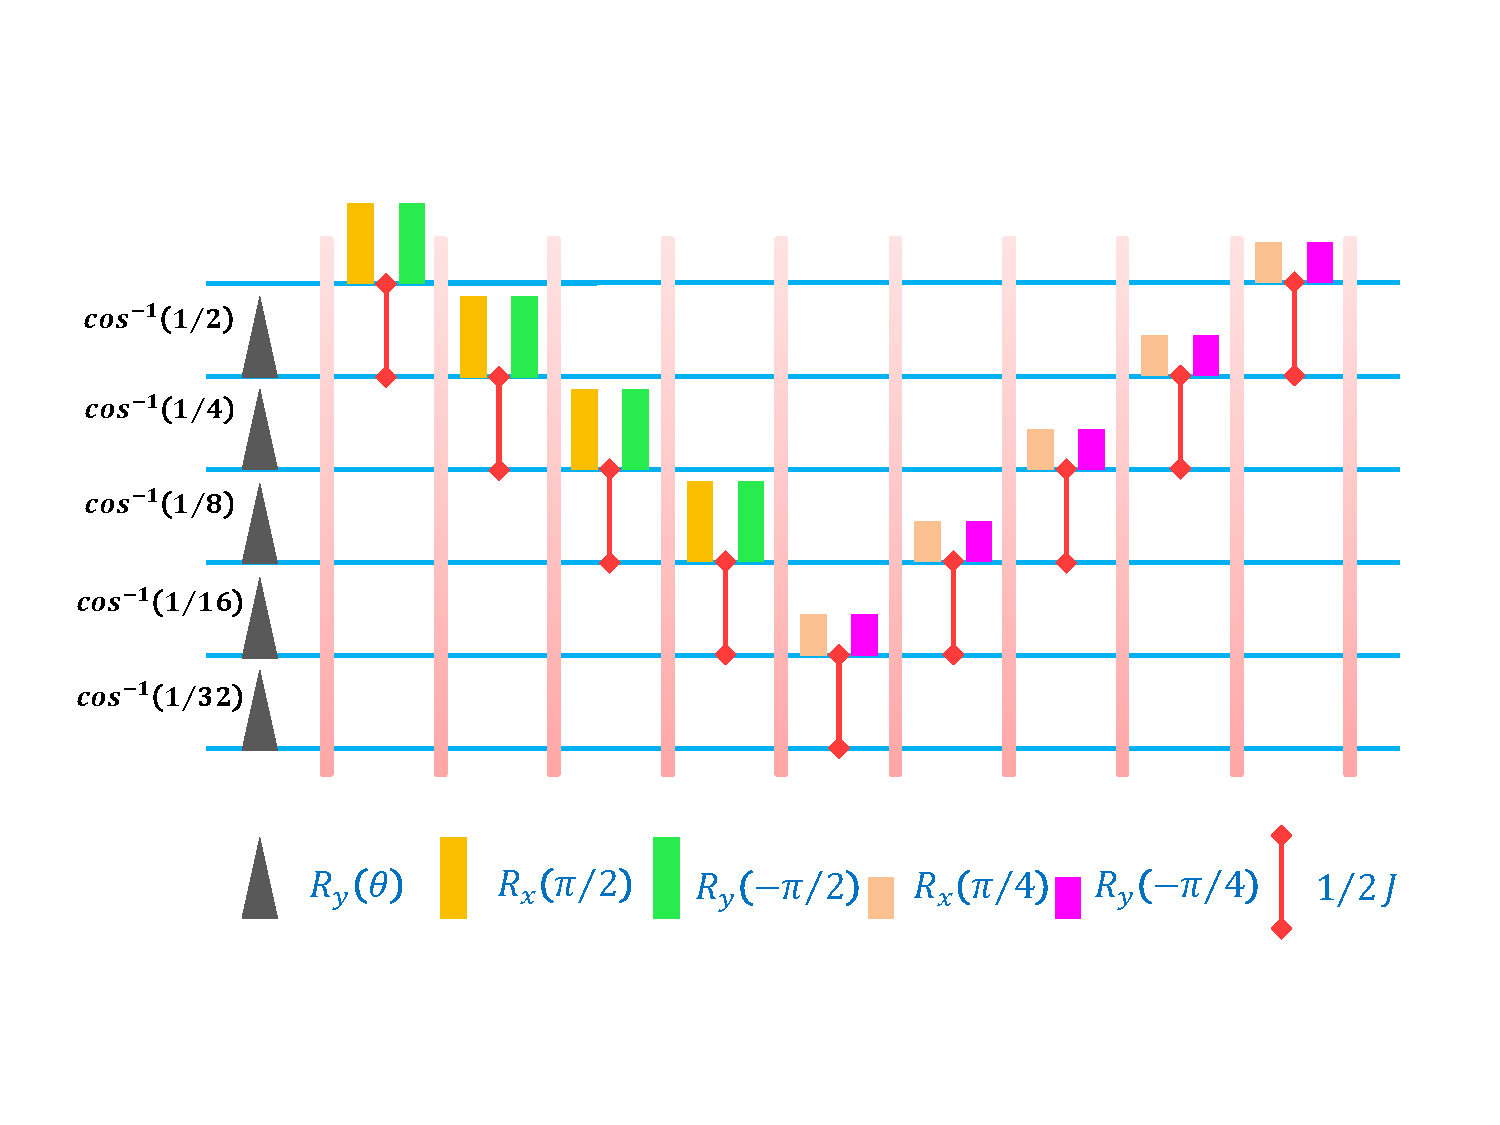
\includegraphics[width= 0.8\columnwidth]{figures/spatial.pdf}
              \caption{可扩展的6 qubit的PPS制备网络图。
              }
              \label{spatial}
            \end{center}
\end{figure}
理论上来说这个网络图是完全可以扩展到任意的$n$个qubit系统的。

(d) \emph{猫态制备法}

猫态制备法\cite{pps3}融合了逻辑标记与空间平均两种方法的思想。它即需要辅助位,也需要梯度场或者相循环来选择高阶相干。
所谓的猫态指的就是最大纠缠态,是以薛定谔的猫来命名的。在3 qubit情况,猫态就是一个GHZ态。从纯态出发,我们可以很轻易地制备猫态,比如四比特时其序列如图\ref{cat}。反过来的话,如果我们可以先制备猫态,自然也就可以得到赝纯态了。

\begin{figure}[htbp]
            \begin{center}
              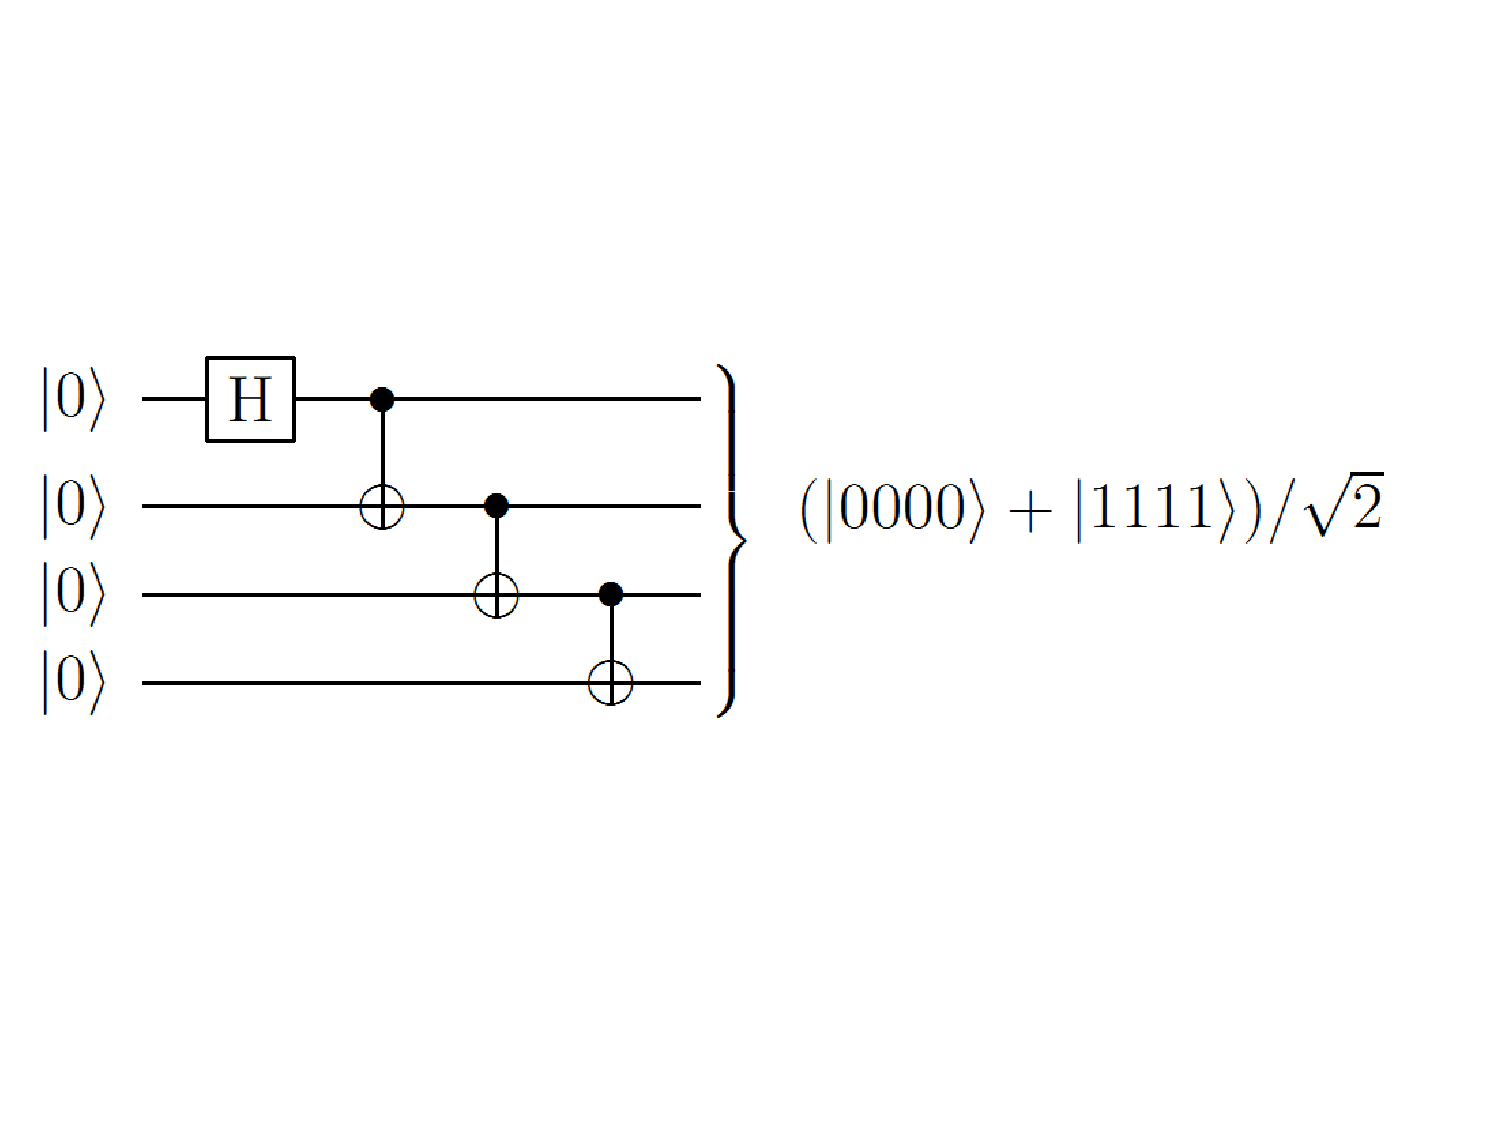
\includegraphics[width= 0.8\columnwidth]{figures/cat.pdf}
              \caption{4 qubit系统上制备猫态的逻辑网络图,仅需要Hadamard操作和CNOT操作。
              }
              \label{cat}
            \end{center}
\end{figure}

让我们考虑更加简单的3 qubit系统。制备猫态的网络图如图\ref{cat3}(a)所示。初态选择为$ZII$的话(这个态可以通过$\pi/2$旋转和梯度场很容易从热平衡态得到),经过该网络后,
系统的末态为$YYX$。该末态是含有三量子相干$ \left\vert 000 \right \rangle \left\langle 111 \right \vert+\left\vert 111 \right \rangle \left\langle 000 \right \vert$的,而这正是一个猫态的形式。在NMR中,不同阶的量子相干对于相位的敏感度是不同的,因此可以通过相循环
或者梯度场的方法把最高阶相干选择出来\cite{pps7}。然后通过图\ref{cat3}(b)所示的解码过程就可以得到逻辑标记的PPS:$X\left\vert 00 \right \rangle \left\langle 00 \right \vert$。

\begin{figure}[htbp]
            \begin{center}
              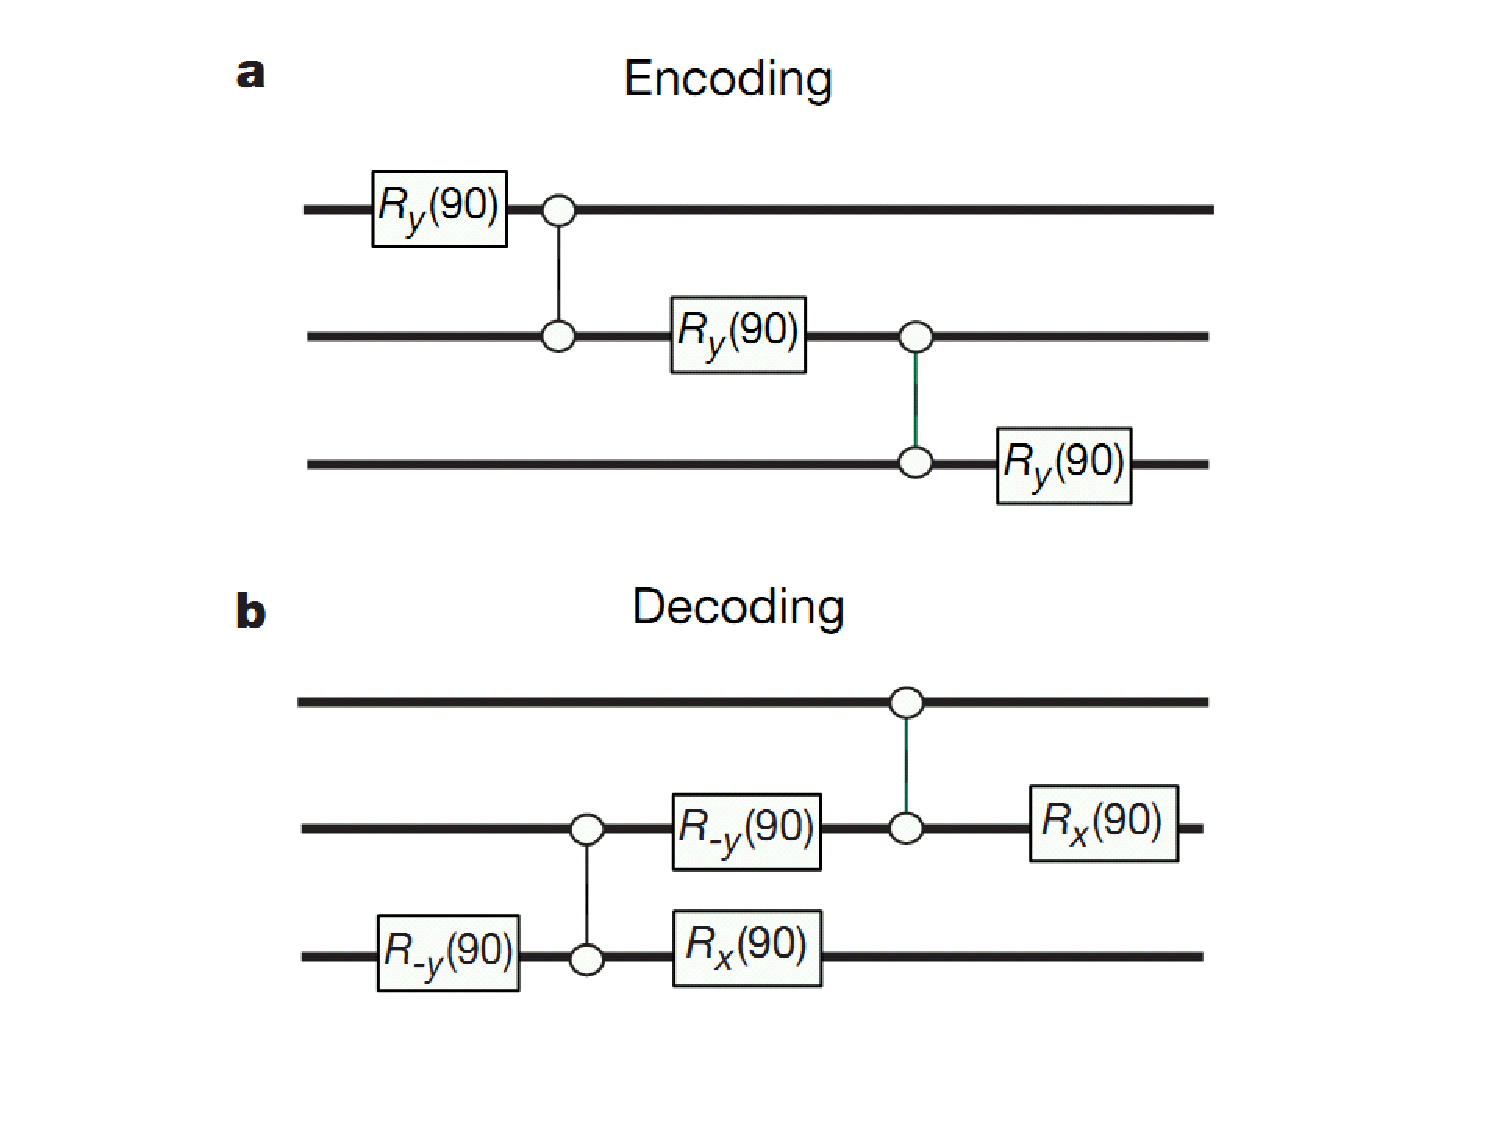
\includegraphics[width= 0.8\columnwidth]{figures/cat3.pdf}
              \caption{3 qubit系统上的猫态PPS制备法。(a) 从初态$ZII$出发,我们可以得到含有三量子相干$ \left\vert 000 \right \rangle \left\langle 111 \right \vert+\left\vert 111 \right \rangle \left\langle 000 \right \vert$的末态$YYX$。(b) 从三量子相干 $\left\vert 000 \right \rangle \left\langle 111 \right \vert+\left\vert 111 \right \rangle \left\langle 000 \right \vert$出发,可以得到逻辑标记后的纯态$X\left\vert 00 \right \rangle \left\langle 00 \right \vert$。取自[Nature 404, 368 (2000) \cite{pps3}]。
              }
              \label{cat3}
            \end{center}
\end{figure}

目前NMR量子计算领域最大qubit的实验就是利用猫态制备法制备了12 qubit的PPS\cite{12qubit},其网络图如图\ref{cat12}。

\begin{figure}[htbp]
            \begin{center}
              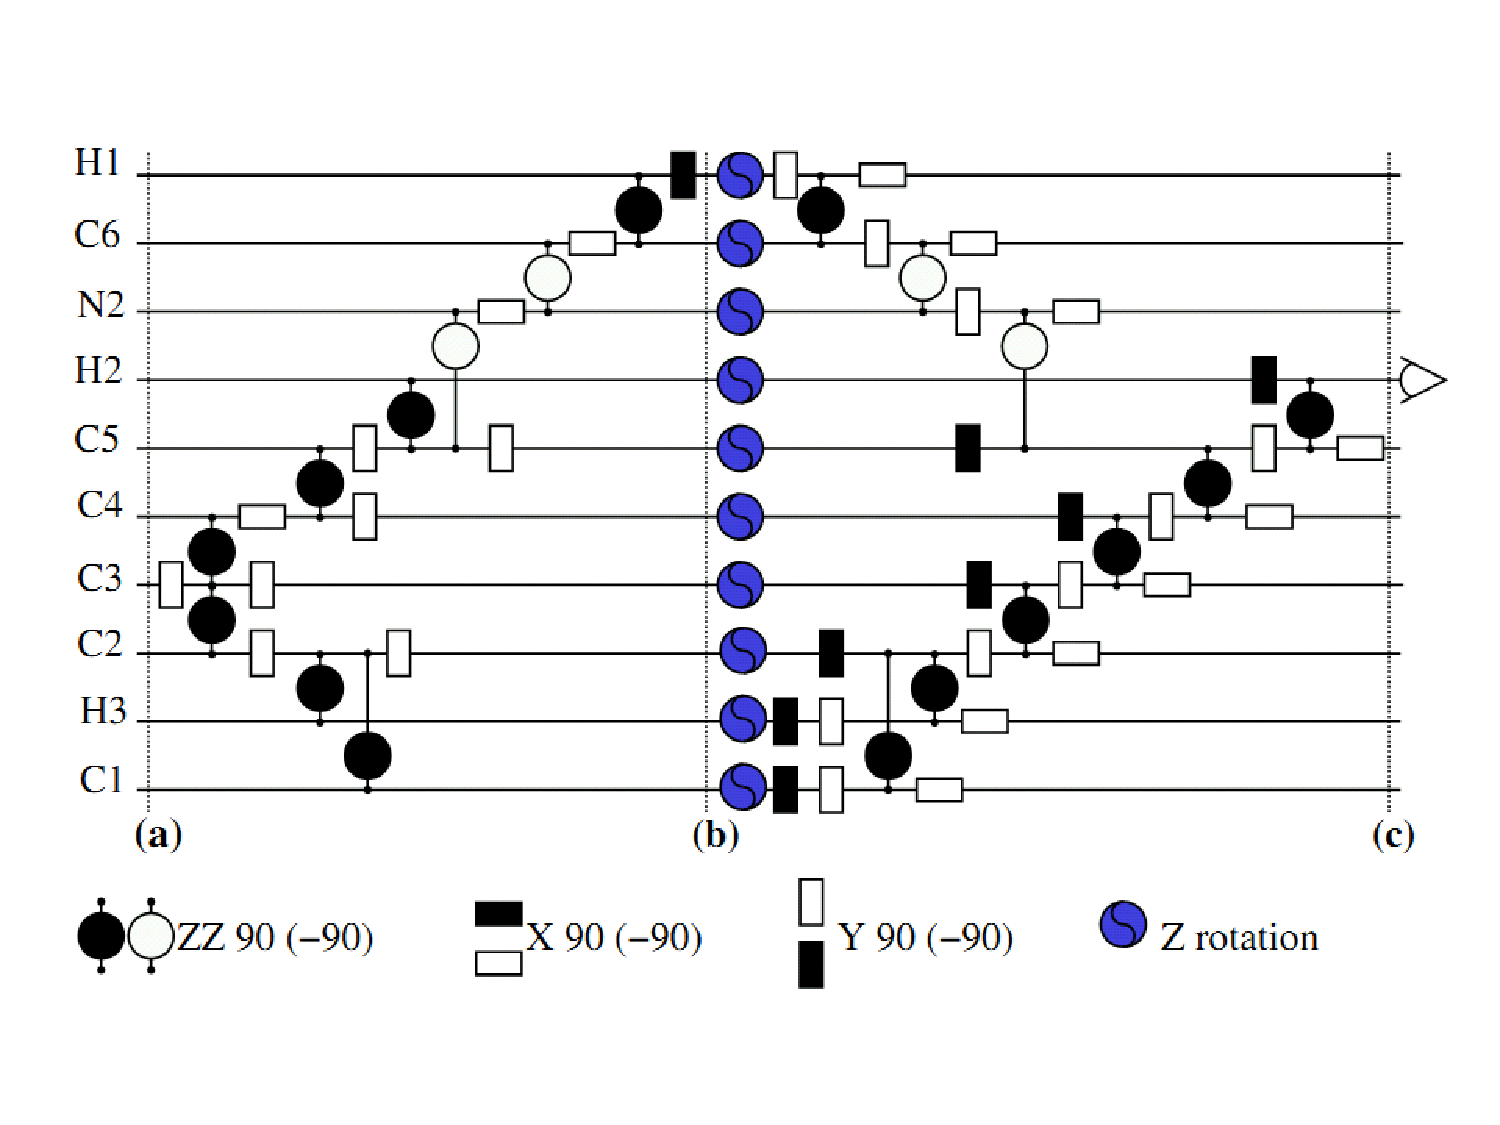
\includegraphics[width= 0.8\columnwidth]{figures/cat12.pdf}
              \caption{12 qubit系统上的猫态PPS制备网络图。取自[Phys. Rev. Lett. 96, 170501 (2006) \cite{12qubit}]。
              }
              \label{cat12}
            \end{center}
\end{figure}

在本节的最后,我们要注意两个问题。首先,所有的PPS制备方案要么对实验数量有指数的要求,要么信号强度会有指数的衰减。造成这种
衰减的原因很简单:这些方案只是简单地把基态能级的布居度选择了出来,而这个布居度的大小是正比于$n/2^n$的。这种指数衰减显然是和
量子计算的宗旨背道而驰的,但是在小量子系统的实验里不会有什么问题。

第二,也是很容易被人忽视的问题,就是我们只是在量子计算任务开始前进行了初态制备。但是很多量子计算方案要求在计算中也能进行
一些初始化过程,比如量子纠错。目前为止,没有合适的方案能做到这一点,当然有些方法原则上可以往这方面扩展。

\subsection{NMR中的读出手段}

单个核自旋的信号是非常难以探测的。目前只有离子阱及NV色心等少数体系中可以通过光学手段进行单自旋探测。在NMR中,我们观测的都是大量系综的统计平均
结果,典型的液体NMR样品大概要包含$10^{18}$个自旋用以观测。对所有的分子来说,它们感受到的操作是相同的,因此所有分子中自旋所处的末态也是相同的,可以进行简单的叠加。

NMR中的探测是通过配置在样品旁边的探测用射频线圈完成的。它可以探测自旋中磁矢量的横向分量,然后把这种时域信号通过傅里叶变化转换成
NMR谱。在NMR中,对于自旋状态的测量是弱测量(weak measurement),也就是探测线圈是一直工作的,但是与核自旋之间的耦合非常弱,因此对退相干几乎没有贡献。当然,由于与热库之间有相互作用以及
静磁场的不均匀性等依然会造成自旋状态的退相干,所以探测到的时域信号是随着时间衰减的,且一般为指数形式。这种由射频线圈采集到的
衰减时域信号叫做自由感应衰减(free induction decay, FID)。

如果FID的衰减形式是$e^{-t/T}$(一般来说$T = T_2^{*}$),那么FID的傅里叶变换将得到一个洛伦兹线型
\begin{equation}\label{aaa}
\propto \frac{1}{1+(\omega-\omega_0)^2}- \frac{i\omega}{1+(\omega-\omega_0)^2},
\end{equation}
且其半高宽为
\begin{equation}\label{aaa}
\Delta f = \frac{\Delta \omega}{2\pi} = \frac{1}{\pi T}.
\end{equation}
由于是弱测量,我们很难得到单个自旋状态的信息。但通过NMR样品中大量全同分子的叠加,我们可以得到想要的
关于平均自旋状态的很多信息。某种程度上来说,这些信息量比投影测量给出的信息量还要大。

测量得到的NMR信号的最大值$V_0$正比于

$\bullet$ 分子数量,与样品的体积$V$和浓度$n_c$有关。

$\bullet$ 分子中的全同原子核的数目$n_e$,比如CH$_3$Cl分子中的$^1$H的数目就为3。

$\bullet$ 热平衡态的自旋极化度$\epsilon_0$,和旋磁比$\gamma$,静磁场$B_0$,以及样品温度$1/T_s$成正比。

$\bullet$ $\omega_0$,与旋磁比$\gamma$和静磁场$B_0$成正比。

$\bullet$ 线圈的品质因子$Q$。

$\bullet$ 填充因子$\eta$,也就是样品在线圈中的占据程度。

$\bullet$ 因子$K$,反应了线圈的几何性质以及线圈与核自旋之间的耦合。

而测量的噪声主要是线圈的热噪声,和以下因素的平方根成正比

$\bullet$ 线圈的绝对温度$T_c$。

$\bullet$ 线路中的分流电阻$R = QL\omega_0$,其中$L$是电感。

$\bullet$ 音频过滤器的带宽$\Delta f$。

同时,NMR中的谱线强度不仅依赖于信号和噪声强度,还和信号在频率上的展宽有关。因此,NMR谱线的信噪比还正比于
$1/m$,$m$为谱线的数目,以及$T_2^{*}$(长的$T_2^{*}$可以给出更窄更高的谱线)。

总的来说,信噪比可以用如下形式表示
\begin{equation}\label{aaa}
\frac{S}{N} \propto \frac{n_cVn_e\gamma^2B_0^2Q\eta KT_2^{*}}{mT_s(T_cQL\gamma B_0\Delta f)^{1/2}} = \frac{n_cVn_e\gamma^{3/2}B_0^{3/2}Q^{1/2}\eta KT_2^{*}}{mT_s(T_cL\Delta f)^{1/2}} .
\end{equation}
关于信噪比的更深入的讨论,可以参见文献\cite{snr1}。

\subsection{NMR中的量子态重构}

对密度矩阵$\rho$的测量可以用来测试或者检验特定的量子态的制备过程。对于$n$个qubit张成的$2^n$维Hilbert空间内的单次测量来说,假定
要测量的态为$\left \vert m \right \rangle$,那么这个单次测量几乎给不出关于$\rho$的任何信息。可以从测量结果$m$推测出来的所有信息就只有
$Pr[\left \vert m \right \rangle]\neq 0$。

如果进行重复测量的话,每次都把系统制备到同样的状态并且在同样的基矢中测量,我们可以得到几率分布
\begin{equation}\label{aaa}
Pr[\left \vert m \right \rangle] =\left \langle m \right \vert \rho \left \vert m \right \rangle = Tr(\rho\left \vert m \right \rangle \left \langle m \right \vert) = Tr(\rho M),
\end{equation}
其中$M$是测量算子。如果我们对每个qubit都在$\{\left \vert 0 \right \rangle, \left \vert 1 \right \rangle\}$ 中重复测量的话,就可以得到密度矩阵中的所有对角元。

量子态重构(quantum state tomography)\cite{tomography1,tomography2,tomography3}是用能够确定出密度矩阵中所有元素的方法。通过在不同的测量基矢下重复测量相同的态,
以及求解线性方程组,我们就可以确定所有的元素。一般来说,我们会通过幺正变换把qubit旋转一个角度,然后在固定的基矢下测量。这和选取不同的基矢是等价的,因为
 \begin{equation}\label{aaa}
Tr[\rho (UMU^{\dagger})] = Tr[(U^{\dagger}\rho U)M].
\end{equation}
比如,单个qubit的密度矩阵可以展开成
 \begin{equation}\label{aaa}
\left(
  \begin{array}{cc}
    \rho_{00} & \rho_{01} \\
    \rho_{10} & \rho_{11} \\
  \end{array}
\right) = \rho_{00} \left \vert 0 \right \rangle \left \langle 0 \right \vert +\rho_{01} \left \vert 0 \right \rangle \left \langle 1 \right \vert+\rho_{10} \left \vert 1 \right \rangle \left \langle 0 \right \vert +\rho_{11} \left \vert 1 \right \rangle \left \langle 1 \right \vert.
\end{equation}
对其在$\{\left \vert 0 \right \rangle, \left \vert 1 \right \rangle\}$中测量的话我们首先可以得到$\rho_{00}$ 及$\rho_{11}=1-\rho_{00}$的值。然后,我们把基矢
绕$\hat{x}$轴转$\pi/2$,把$\rho$转化成$X\rho X^{\dagger}$,我们就可以得到$Im(\rho_{10}) = -Im(\rho_{01})$。类似地,绕$\hat{y}$轴转$\pi/2$ 的话我们可以得到$Re(\rho_{10}) = Re(\rho_{01})$。因此,三次测量就可以让我们重构整个密度矩阵$\rho$。

对于$n$个qubit的体系,我们也可以把密度矩阵展开为
\begin{equation}\label{aaa}
\rho = \sum_{i = 0}^{2^n-1}\sum_{j=0}^{2^n-1} \rho_{ij}\left \vert i \right \rangle \left \langle j \right \vert,
\end{equation}
并选择一组基矢变换,可以得到$\rho$中的所有$4^n-1$个自由度。

如果我们选择利用Pauli基组而不是计算基矢展开的话,找到基矢变换会更加容易。对单qubit的密度矩阵,它的Pauli展开可以写成
\begin{equation}\label{aaa}
\rho = c_0 \sigma_0+c_1 \sigma_1+c_2 \sigma_2+c_3 \sigma_3,
\end{equation}
其中$c_0=1$为归一化条件,且$\sigma_0 = I/2, \sigma_1 = \sigma_x/2,\sigma_2 = \sigma_y/2,\sigma_3 = \sigma_z/2$。在计算基矢中的测量给出$Pr[\left \vert 0 \right \rangle] = (c_0+c_3)/2$,且 $Pr[\left \vert 1 \right \rangle] = (c_0-c_3)/2$ ,我们就可以解出$c_3$。而由于
\begin{eqnarray}\label{aaa}
X\rho X^{\dagger} = c_0 \sigma_0+c_1 \sigma_1-c_3 \sigma_2+c_2 \sigma_3, \nonumber \\
Y\rho Y^{\dagger} = c_0 \sigma_0+c_3 \sigma_1+c_2 \sigma_2-c_1 \sigma_3,
\end{eqnarray}
我们就可以在施加$X$后得到$(c_0\pm c_2)/2$,而在施加$Y$后得到$(c_0\mp c_1)/2$。

对于$n$个qubit,Pauli展开可以写成
\begin{equation}\label{aaa}
\rho = \sum_{i =0}^3  \sum_{j =0}^3 \cdots \sum_{k =0}^3 c_{ij\cdots k} \sigma_i\otimes \sigma_j \otimes\cdots \otimes \sigma_k,
\end{equation}
其中$c_{00\cdots 0}=1$为归一化条件。在计算基矢中的测量算子由以下形式给出
\begin{equation}\label{aaa}
(\sigma_0 \pm \sigma_3) \otimes (\sigma_0 \pm \sigma_3)\otimes\cdots \otimes (\sigma_0 \pm \sigma_3),
\end{equation}
并给出相应的概率
\begin{equation}\label{aaa}
\sum_{i,j,\ldots,k\in \{0,3\}} \pm \frac{c_{ij\cdots k}}{2^n}.
\end{equation}
例如对于2 qubit体系,有
\begin{eqnarray}\label{aaa}
Pr[\left \vert 00 \right \rangle] = (c_{00}+c_{03}+c_{30}+c_{33})/4, \\
Pr[\left \vert 01 \right \rangle] = (c_{00}-c_{03}+c_{30}-c_{33})/4,\\
Pr[\left \vert 10 \right \rangle] = (c_{00}+c_{03}-c_{30}-c_{33})/4,\\
Pr[\left \vert 11 \right \rangle] = (c_{00}-c_{03}-c_{30}+c_{33})/4,
\end{eqnarray}
这样我们就可以通过求解线性方程组得到$c_{03},c_{30},c_{33}$。然后,要得到其他的$c_{ij\cdots k}$的话我们则需要进行旋转,比如
\begin{equation}\label{aaa}
X_1Y_2(\sigma_0 + \sigma_2)\otimes(\sigma_0 + \sigma_1)X_1^{\dagger}Y_2^{\dagger} = (\sigma_0 + \sigma_3)\otimes(\sigma_0 - \sigma_3).
\end{equation}

最后要说的是,测量基矢并非一定要选择计算基矢,在NMR实验中,单qubit测量算子可以写成$-i\sigma_1 - \sigma_2$。而对于耦合起来的两个自旋,测量算子为
\begin{eqnarray}\label{opernmr}
2(-i\sigma_1 - \sigma_2)\otimes (\sigma_0 \pm \sigma_3),\\
(\sigma_0 \pm \sigma_3) \otimes 2(-i\sigma_1 - \sigma_2).
\end{eqnarray}
由于NMR的实验结果是大量分子的系综平均,这些算子的期望值可以通过单次的NMR谱线直接读出。
式\ref{opernmr}中的四个算子就对应于两自旋系统的四条NMR谱线,而相位测量则允许我们同时读出每条谱线的实部和虚部项,从而区分$\sigma_1$和$\sigma_2$的贡献。

在测量出末态后,我们需要对实验上测到的结果$\left \vert \phi \right \rangle$和理论预期$\left \vert \psi \right \rangle$进行比较。对于这点我们引入量子态保真度(quantum state fidelity)的概念。对于两个纯态 的情况,保真度的定义为
\begin{equation}\label{aaa}
F(\left \vert \psi \right \rangle, \left \vert \phi \right \rangle) = |\left \langle \phi | \psi \right \rangle|,
\end{equation}
简单来说就是两个态交叠程度的绝对值的大小。

更一般的情况,末态使用密度矩阵来表示的,因为密度矩阵语言可以描述由于退相干导致的量子态的混合,即混态。
描述一个纯态$\left \vert \psi \right \rangle$和混态$\rho$的保真度形式为
\begin{equation}\label{erty}
F(\left \vert \psi \right \rangle, \rho) = \sqrt{\left \langle \psi \right \vert \rho   \left \vert \psi \right \rangle},
\end{equation}
当$\rho =\left \vert \phi \right \rangle\left \langle \phi \right \vert $时这个形式就退化到两个纯态的情况。

而对于两个混态$\rho$和$\sigma$来说,它们之间的保真度则定义为
\begin{equation}\label{aaa}
F(\sigma, \rho) = Tr \sqrt{\sqrt{\sigma}\rho\sqrt{\sigma}}.
\end{equation}
在这个表达式中其实$\rho$和$\sigma$是对称的,而其中一个为纯态时就退化到了式\ref{erty}的情况。

实验上另外一个常用的衡量保真度的参数是相关性(correlation),其形式为
\begin{equation}\label{correlation}
C = \frac{Tr(\sigma \rho)}{\sqrt{Tr(\sigma^2)Tr(\rho^2)}}.
\end{equation}
一般来说,相关性的值要比保真度高一些。

\section{强耦合液晶NMR体系量子计算}

前面的章节我们主要集中于讨论耦合形式为$I^i_zI^j_z$形式的哈密顿量模型,也就是弱耦合近似下的$J$耦合模型。
液体中由于分子的快速滚动,偶极耦合的效果都被平均掉了,而液晶及固体样品中偶极耦合的效应会显现,导致其处理手段和液体NMR有很大的不同。本节我们就将着重分析如何
利用强耦合NMR体系进行量子计算,主要集中在液晶NMR体系。

\subsection{强耦合体系的处理方法}

在液晶体系中,偶极耦合的大小约为$0$到$20kHz$,这个值远大于J耦合的$0$到$200Hz$的量级。因此对于自旋$1/2$的液晶体系,其哈密顿量形式为
\begin{equation}\label{aaa}
H_{sys}=\hbar\sum_{i} \omega_i I_z^i + \hbar\sum_{i<j} 2\pi J_{ij}I_z^iI_z^j + \sum_{i<j} \pi D_{ij}(2I_z^iI_z^j-I_x^iI_x^j-I_y^iI_y^j),
\end{equation}
$D_{IJ}$是核自旋$i$和$j$之间的偶极耦合常数。在偶极耦合项中,由于存在两个和其他项不对易横向分量$I_x^iI_x^j$和$I_y^iI_y^j$,
才使液晶NMR体系展现出很多和液体不一样的性质。

考虑简单的两体情况并忽略掉$J$耦合,则哈密顿量可以简化为(省略$\hbar$)
\begin{equation}\label{aaa}
H_{sys}=\omega_1 I_z^1+\omega_2 I_z^2 +  \pi D_{12}(2I_z^1I_z^2-I_x^1I_x^2-I_y^1I_y^2),
\end{equation}
写成矩阵形式的话
\begin{equation}\label{aaa}
H_{sys}=\left(
          \begin{array}{cccc}
            H_{11} &   &   &   \\
              & H_{22}   & H_{23}   &   \\
              &   H_{32} & H_{33}   &   \\
              &   &   & H_{44}   \\
          \end{array}
        \right),
\end{equation}
其中
\begin{eqnarray}\label{aaa}
H_{11}& =& +\frac{1}{2}\omega_1 +\frac{1}{2}\omega_2+\frac{1}{2}\pi D, \nonumber \\
H_{22}& =& +\frac{1}{2}\omega_1 -\frac{1}{2}\omega_2-\frac{1}{2}\pi D, \nonumber \\
H_{33}& =& -\frac{1}{2}\omega_1 +\frac{1}{2}\omega_2-\frac{1}{2}\pi D, \nonumber \\
H_{44}& =& -\frac{1}{2}\omega_1 -\frac{1}{2}\omega_2+\frac{1}{2}\pi D, \nonumber \\
H_{23}& =& H_{32}  =-\frac{1}{2}\pi D.
\end{eqnarray}

该形式的四个本征态分别为$\left \vert \alpha\alpha \right \rangle$,$cos\theta \left \vert \alpha\beta \right \rangle+sin\theta \left \vert \beta\alpha \right \rangle$,$cos\theta \left \vert \beta\alpha \right \rangle-sin\theta \left \vert \alpha\beta \right \rangle$,$\left \vert\beta\beta \right \rangle$。这里
\begin{equation}\label{aaa}
tan(2\theta) = \frac{-\pi D}{\omega_1-\omega_2}.
\end{equation}

很自然地可以看出,这四个本征态不再是四个计算基态。我们把这四个态标记为量子计算中的
$\left \vert 00 \right \rangle$,$\left \vert 01 \right \rangle$,$\left \vert 10 \right \rangle$,$\left \vert11 \right \rangle$态的话,这依然是一个两比特体系。这样标记的好处是NMR的谱线对应的是两个本征态之间的跃迁,
那么和液体NMR中采用核自旋作为qubit的标记一样,每条谱线只会与量子计算中的两个能级相关,因此更加直观。当然,在这种标记方式下,核选脉冲的意义
将变得不明显,而线选脉冲由于是对一个跃迁进行操作,因此将发挥更大的作用。更加方便的是用SMP或者GRAPE脉冲,它们的精度会更高。同时注意一点,当附加一个
能够使哈密顿量对角化的幺正操作后,其实这两种标记方式是等价的。

该哈密顿量的四个本征态所对应的本征值分别是
\begin{eqnarray}\label{aaa}
E_1  &=& -\frac{1}{2}\omega_1 -\frac{1}{2}\omega_2+\frac{1}{2}\pi D, \nonumber \\
E_2& =& +\frac{1}{2} \sqrt{(\omega_1 - \omega_2)^2+\pi^2D^2}-\frac{1}{2}\pi D, \nonumber \\
E_3& =& -\frac{1}{2}\sqrt{(\omega_1 - \omega_2)^2+\pi^2D^2}-\frac{1}{2}\pi D, \nonumber \\
E_4 & =& +\frac{1}{2}\omega_1 +\frac{1}{2}\omega_2+\frac{1}{2}\pi D,
\end{eqnarray}
通过本征值我们可以得到NMR谱线中各条谱峰的位置为
\begin{equation}\label{aaa}
 +\frac{1}{2}\omega_1 +\frac{1}{2}\omega_2\pm\frac{1}{2}\pi D \pm \frac{1}{2} \sqrt{(\omega_1 - \omega_2)^2+\pi^2D^2}.
\end{equation}
而这四条谱峰的高度将正比于$(cos\theta+sin\theta)^2$,$(cos\theta-sin\theta)^2$。当$\pi D\ll \omega_1 - \omega_2$,也就是$tan(2\theta)\approx 0 $时,我们发现四条谱峰依然等高,这就退化到了液体NMR中的弱耦合近似情况。

\subsection{液晶NMR量子计算的具体过程}


在了解到哈密顿量形式及本征值和本征态的不同后,下一点就是液晶NMR中哈密顿量的各个参数的确定。和液体情况不同,液晶样品的哈密顿量形式
中由于所有项并不是两两对易的,我们不可能
在简单地通过热平衡态的NMR谱线得到其数值大小了。比较原始的确定哈密顿量各个参数的办法是通过二维Z-COSY实验\cite{lq2}。我们采用的是拟合的办法,其步骤如下:

1. 把样品溶于液体溶剂Acetone中,测出$J$耦合的大小,并将其代入哈密顿量形式中作为已知参数。

2. 对哈密顿量中的化学位移及偶极耦合常数作初始猜测,然后计算该猜测的哈密顿量形式对应的NMR热平衡谱中各条谱线的位置。

3. 把计算出来的各条谱线同实验上各条谱线的位置进行平方差求和运算,以确定两者之间的误差大小。如果足够小(1Hz之内),则保留这组参数,否则对当前的哈密顿量参数进行
扰动,并重新计算谱线。

4. 在得到所有参数后,我们将计算NMR谱线的强度并与实验结果对比,作为除谱线位置外的另一组对比参数。我们发现只要谱线位置符合的话,谱线强度也符合的很好。

目前,我们已经在2,3,4 qubit的液晶体系上实现了哈密顿量的解谱,并保证满足液晶中的序参量与几何性质要求\cite{lq1}。同时,这些样品上也都完成了PPS制备,以及执行了相应的量子计算任务,并得到了很好的实验结果。这些都说明
我们的解谱确定哈密顿量参数的过程是正确的。

当前实验室内常用的液晶样品包括:2 qubit的1-bromo-2,3,5-dichloro-benzene,3 qubit的3-bromo-1,2-dichloro-benzene,以及4 qubit的1-bromo-2-dichloro-benzene。所有溶剂均为ZLI1132液晶溶剂。这些样品其实是把苯环上的六个$^1$H用没信号的$Br$或者$Cl$代替,
而剩下的$^1$H由于化学结构上不对称就可以作为两能级的qubit使用,它们的结构图如图\ref{lqsample}所示。

\begin{figure}[htbp]
            \begin{center}
              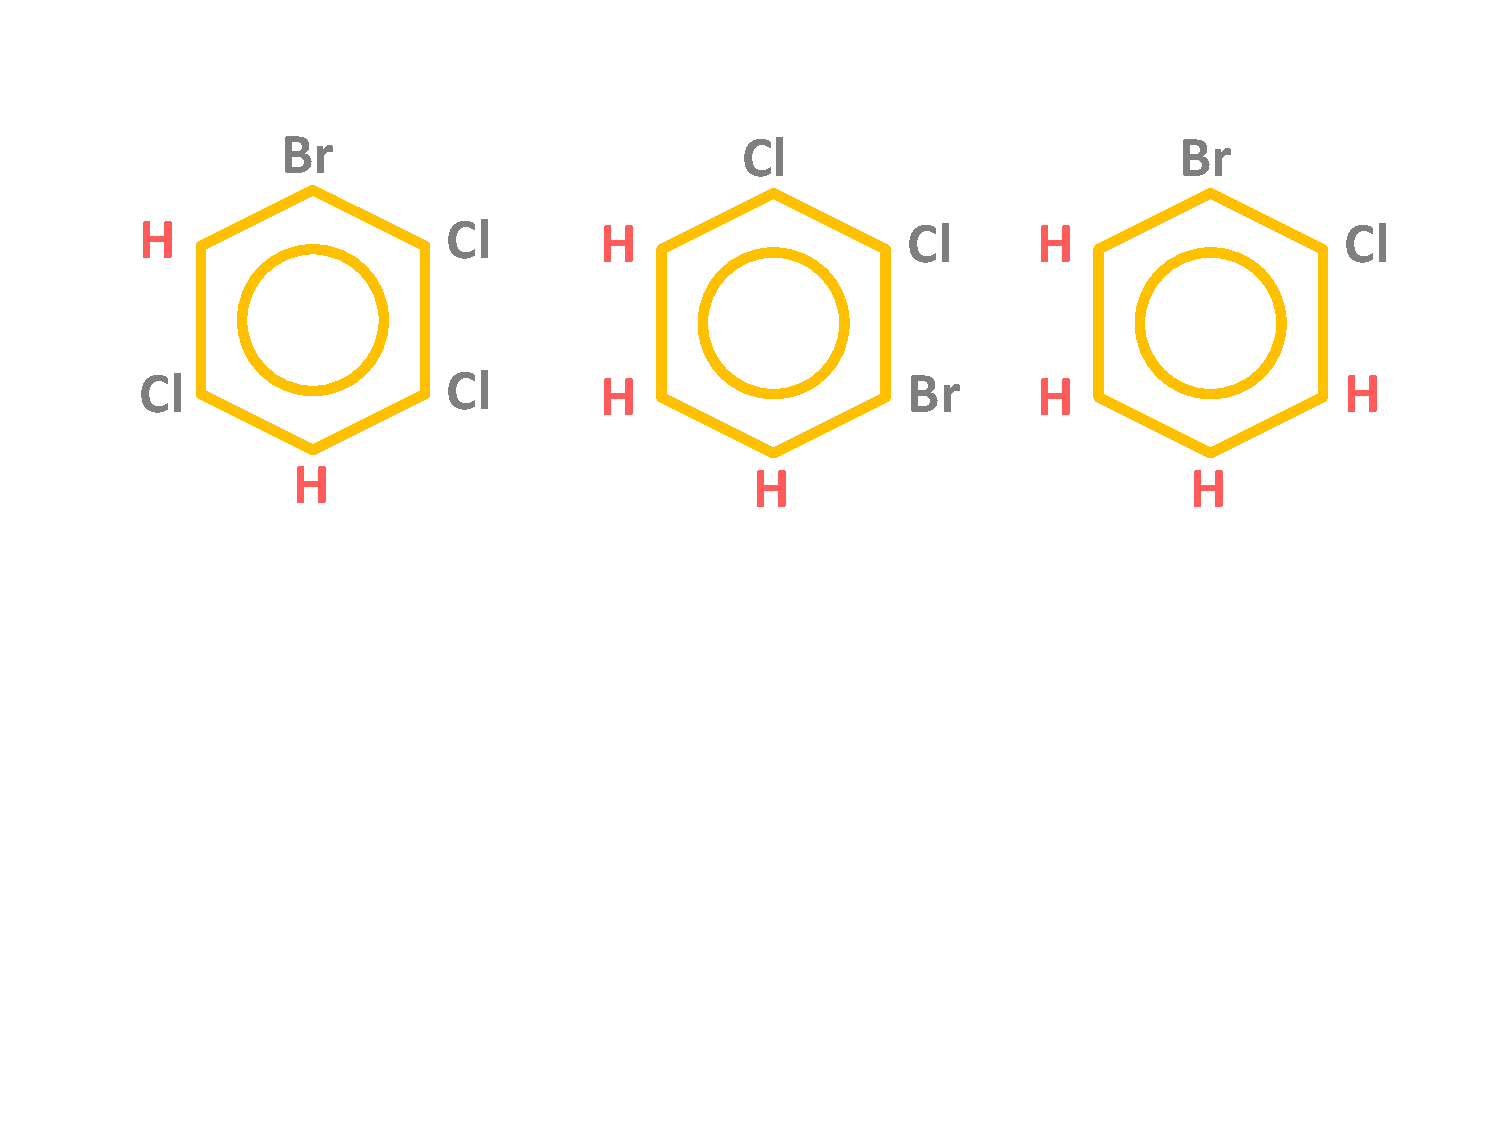
\includegraphics[width= 0.8\columnwidth]{figures/lqsample.pdf}
              \caption{2, 3, 4 qubit的液晶样品结构。苯环上的$^1$H被用作qubit。
              }
              \label{lqsample}
            \end{center}
\end{figure}

NMR量子计算的第一步是PPS制备,液晶样品也不例外。除了前面提到过的液体NMR中各种PPS制备方法,针对液晶体系特殊的哈密顿量形式
又有一些新的技巧,比如线选脉冲饱和能级\cite{lq3},制备PPS对\cite{lq4,lq5,lq6}等。这些方法都有着或多或少的局限性。
借助于GRAPE脉冲,我们设计了基于GRAPE搜索的PPS制备方法,其基本思路为
\begin{equation}\label{aaa}
\sum_i I^i_z \rightarrow U\rightarrow Gz \rightarrow\rho_{pps}.
\end{equation}
可以看出,我们只用了一个幺正操作和一个梯度场,就可使实现PPS。该方法的核心在于如何找到这样一个操作$U$,并把它写成脉冲的形式。

首先我们把$U$分割,即
\begin{equation}\label{aaa}
U = U_N U_{N-1}\cdots U_1,
\end{equation}
其中
\begin{equation}\label{aaa}
U_j = e^{-i\Delta t ((H_{int} + \sum_{k=1}^mu_k(j)H_{ext})}.
\end{equation}

对于PPS,我们设其理论形式为
\begin{equation}\label{aaa}
\rho_{th} = \left \vert 0\ldots 0 \right \rangle \left \langle 0\ldots 0 \right \vert - \frac{I}{2^n},
\end{equation}
$n$为qubit的数目。在施加了GRAPE脉冲及梯度场后,我们的末态为
\begin{equation}\label{aaa}
\rho_{exp} = Gz(U \rho_{in} U^{\dagger}).
\end{equation}

为了衡量$\rho_{exp} $和$\rho_{th}$之间的相似程度,我们采用了式\ref{correlation}定义的相关性
\begin{equation}\label{correlation}
C = \frac{Tr(\rho_{exp} \rho_{th})}{\sqrt{Tr(\rho_{exp}^2)Tr(\rho_{th}^2)}}.
\end{equation}

假设
\begin{equation}\label{aaa}
U = U_B U_{j} U_A,
\end{equation}
且$U_A = U_{j-1}\cdots U_1$,$U_B = U_N\cdots U_{j+1}$。我们对幅度因子$u_j$进行一个微扰$\Delta u_j$后,可以得到相关性$C$感受到的微扰$\Delta C_j$,然后我们就可以进行新的梯度修正
\begin{equation}\label{aaa}
u_j \rightarrow u_j + \epsilon \frac{\Delta C_j}{\Delta u_j}.
\end{equation}
这个思路和GRAPE脉冲的思想非常类似,而通过循环搜索,我们可以得到保真度很高的GRAPE脉冲。
例如,在4 qubit液晶体系,我们可以得到2000$\mu s$,分为400小片,保真度为0.97的GRAPE脉冲。

在完成了PPS制备后,我们要考虑如何有效地在液晶体系上进行幺正演化。注意到液晶的哈密顿量不是对角的,
一个很自然的想法是把它进行对角化
\begin{eqnarray}\label{aaa}
U^{\dagger} H U = H_D, \nonumber \\
UH_DU^{\dagger}  = H.
\end{eqnarray}
其中$H_D$指的是对角化后的哈密顿量,对应于液体NMR中的形式。必须提到矩阵对角化在经典计算上本身是一个多项式难的问题,所以这一步其实仅在低量子位有效。而哈密顿量对角化的量子算法可以参见文献\cite{lq7}。

在对角化之后,我们发现经过这个幺正变换$U$后液晶体系的读出和液体居然是一样的,因为
\begin{eqnarray}
&&Tr(e^{-iH_Dt}R\rho R^{\dagger}e^{iH_Dt}\cdot F^{+}) \nonumber \\
&=&Tr(Ue^{-iH_Dt}U^{\dagger}\cdot  URU^{\dagger} \cdot  U \rho U^{\dagger}  \cdot  U  R^{\dagger} U^{\dagger} \cdot  U e^{iH_Dt} U^{\dagger}  \cdot  U  F^{+} U^{\dagger}) \nonumber \\
&=&Tr(e^{-iHt}\cdot  URU^{\dagger} \cdot  U \rho U^{\dagger}  \cdot  U  R^{\dagger} U^{\dagger} \cdot  e^{iHt} \cdot  F'^{+} ).
\end{eqnarray}
那么,我们只要把液体NMR中的初态$\rho$和幺正操作$R$转化到液晶体系中就可以了,需要的仅仅是把初态变为
$U \rho U^{\dagger}$,操作变为$ URU^{\dagger}$。

液晶NMR的读出和逻辑操作类似,只要把用于液体的重构序列进行一个幺正变换$U$即可,而其测量方式和液体NMR完全相同。

最后整理下液晶NMR量子计算的步骤。

$\bullet$ 测量液晶样品的热平衡谱,并解谱得到哈密顿量形式。

$\bullet$ 求解其本征值和本征态,并进行对角化操作,得到用来对角化的操作$U$及对角化后的哈密顿量$H_D$。

$\bullet$  假定量子计算实验是在液体NMR样品$H_D$中完成的,并设计在该样品完成时如何进行初态制备,逻辑操作,结果读出等。

$\bullet$ 把$H_D$中所有的操作前面都施加幺正变换$U$,再移植到液晶样品中。由于$U$的形式一般不规律,最好是通过SMP或是GRAPE脉冲算出。

$\bullet$  液晶中所有的测量读出脉冲也和液体类似,只不过加上幺正变换$U$。

为了证明以上思路的可行性,接下来我们将以一个4 qubit液晶NMR实验为例具体讲解。

\subsection{利用4 qubit液晶样品绝热分解143}

前面已经提到,最能代表量子计算优越性的算法是Shor的大数分解算法\cite{Shor},但实验上想验证Shor算法是非常困难的。
最早的实验是2000年利用7 qubit
NMR样品分解了15\cite{shor15},这也是NMR量子计算早期的代表工作。后来,我们组提出了基于绝热的量子分解算法,需要的资源更少,复杂度也更低,并在3 qubit样品上成功分解了21\cite{shor21},光学体系也相继分解了15\cite{optshor15}。最近,我们改进了自己提出的绝热分解算法,设计了4 qubit分解143的实验方案,并在4 qubit液晶NMR样品上完成了这一实验\cite{shor143}。本节我们就将主要介绍该实验过程。

首先简要介绍一下绝热量子计算(adiabatic quantum computing, AQC)\cite{aqc1}。在AQC的框架中,量子体系首先被制备到初始哈密顿量$H_0$的基态,而量子计算任务的答案则蕴含在最终哈密顿量$H_p$的基态里。
在计算过程冲,含时的哈密顿量非常缓慢地从$H_0$变化到$H_p$,保证量子体系一直处于当前哈密顿量的基态上。最后,通过测量末态,也就是$H_p$的基态,
我们就可以得到问题的解。最简单的哈密顿量变化形式是如下插值
\begin{equation}\label{aaa}
H(t) = [1-s(t)]H_0+s(t)H_p,
\end{equation}
其中$s(t)$从0缓慢地变化到1。AQC比较适合的是求解最优化问题,因为很多最优的解都是蕴含在哈密顿量的基态中。

对于大数的分解问题,我们可以用$N = p\times q$给出,$p$和$q$是$N$的两个质因子。设计AQC的核心在于如何把这样一个等式转化为最优化问题,最直接的想法是通过
等式$N - pq = 0$来构造函数$f(x,y) =(N - xy)^2$。$f(p,q)=0$肯定是这个函数的最小值,也是其最优解。那么,末态哈密顿量就可以选择为
\begin{equation}\label{interpo}
H_p = (N - \hat{x}\times\hat{y})^2,
\end{equation}
其中,$\hat{x}$用$\sum_{i = 0}^{n-1}2^i(\frac{1-\sigma_z^i}{2})$来构造,且$n$为$x$转化为二进制时的比特数。算子$\hat{y}$也可以类似构造。那么,
$H_p$的基态能量就为0,代表$N = p\times q$。NMR上进行的21分解的实验就是用这种构造方式完成的\cite{shor21}。

在上述方案中,末态哈密顿量的能谱宽度是和要分解的数$N$成线性关系的,因此当$N$很大时,实验上很难找到如此具有如此大
能谱宽度的哈密顿量。后来,Schaller和 Sch\"{u}tzhold\cite{aqc2,aqc3}利用求解线性方程组的方法优化了这个问题。在143分解中,我们把$N = p\times q$转化为二进制形式的乘法,并用图\ref{linearset}中所示的二进制乘法表列出一系列的方程,构成线性方程组。可以看到,
目标问题把确定质因子$p$和$q$转化为确定二进制数$p_1,p_2$和$q_1,q_2$,然后把二进制数$1p_2p_11$和$1q_2q_11$转化为十进制即可。

\begin{figure}[htbp]
            \begin{center}
              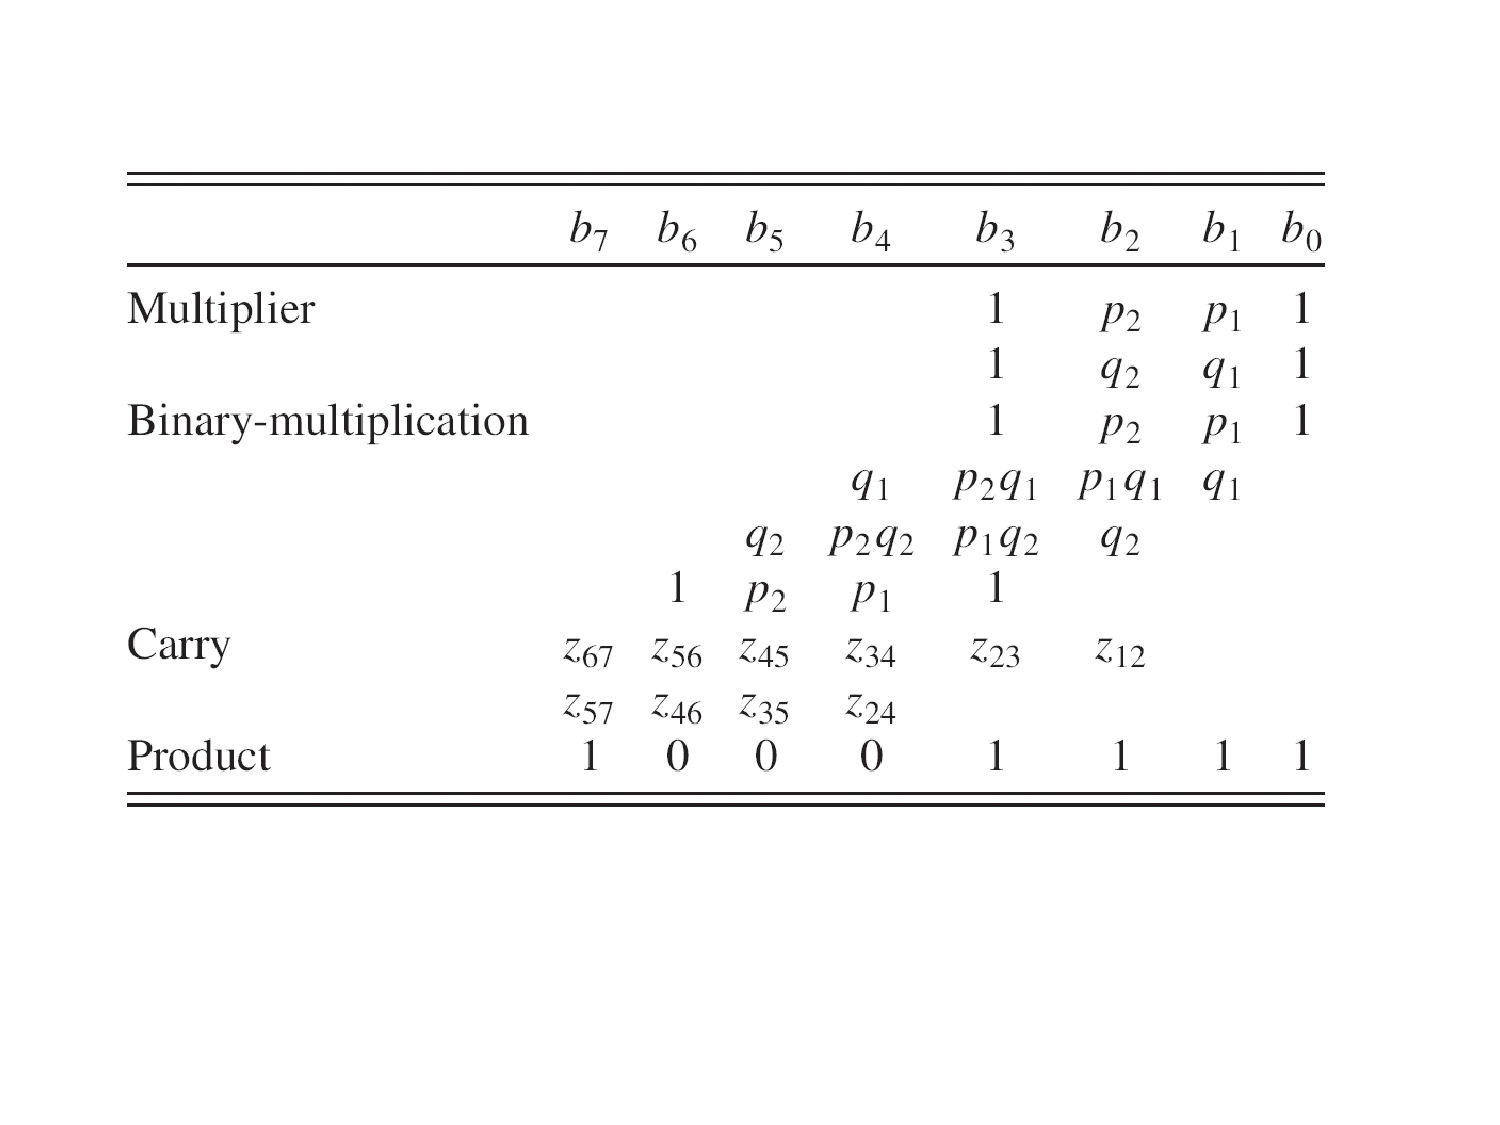
\includegraphics[width= 0.8\columnwidth]{figures/linearset.pdf}
              \caption{$N = 143$分解中用到的二进制乘法表。$N = p\times q$中的所有数值都被转化为了二进制,然后利用这个乘法结构可以列出一个线性方程组。
              }
              \label{linearset}
            \end{center}
\end{figure}

通过约束条件化简该线性方程组后(具体过程请参见文章\cite{shor143}),我们得到目标,也就是末态哈密顿量的形式为
\begin{eqnarray}
H_p &=& 5-3 \hat{p}_1-\hat{p}_2-\hat{q}_1+2 \hat{p}_1 \hat{q}_1-3 \hat{p}_2 \hat{q}_1\nonumber\\
&+&2 \hat{p}_1 \hat{p}_2 \hat{q}_1-3 \hat{q}_2+\hat{p}_1
\hat{q}_2+2\hat{p}_2 \hat{q}_2+2 \hat{p}_2 \hat{q}_1
\hat{q}_2,\label{hp}
\end{eqnarray}
其中$\hat{p}$ 和 $\hat{q}$被映射到了qubit空间$\hat{p}_1=\frac{1-\sigma_z^1}{2},
\hat{p}_2=\frac{1-\sigma_z^2}{2}, \hat{q}_1=\frac{1-\sigma_z^3}{2}$,$ \hat{q}_2=\frac{1-\sigma_z^4}{2} $。

绝热演化的初始哈密顿量可以选择容易制备其初态的哈密顿量形式,例如这里选择的是
\begin{equation}\label{aaa}
H_0=g(\sigma_{x}^{1}+\sigma_{x}^{2}+\cdots+\sigma_{x}^{n}).
\end{equation}
该哈密顿量的基态形式为所有计算基矢的叠加,即
\begin{equation}\label{aaa}
\left \vert \psi_i \right \rangle=\left(
\frac{|0\rangle-|1\rangle}{\sqrt{2}} \right)^{\otimes n}.
\end{equation}
在计算过程中,首先我们把量子体系制备到$H_0$的基态$|\psi_i\rangle$上,然后依据插值公式\ref{interpo}把$H_0$
缓慢地变化到$H_p$,绝热定理保证系统始终处于当前哈密顿量的基态上。最后,通过测量末态的形式,我们可以得到
二进制数$p_1,p_2$和$q_1,q_2$,从而得到
143分解问题的解。该过程的数值模拟可以参加图\ref{143sim}(a)。

\begin{figure}[htbp]
            \begin{center}
              \includegraphics[width= 0.8\columnwidth]{figures/143sim.pdf}
              \caption{(a) 143分解中,最低的三个能级变化的示意图。初始哈密顿量中的$g$因子设为0.6。(b) $k = 1-5$对应图(a)中5个点的布居度分布。$k = 6$则是实验上得到的末态的布居度分布。可以看到,最终所有的布居度几乎都处于
              $\left \vert 0110 \right \rangle \left \langle 0110 \right \vert$和$\left \vert 1001 \right \rangle \left \langle 1001 \right \vert$上,表示143分解的结果为$p =11,q=13$或者$p = 13,q=11$。}
              \label{143sim}
            \end{center}
\end{figure}

在实验上,我们选择了4 qubit液晶样品1-bromo-2-dichloro-benzene(图\ref{143sample}(a))溶于ZLI1132作为量子体系。样品中的四个$^1$H
核自旋作为四个qubit,其哈密顿量形式为
\begin{equation}
 \mathcal{H} = 2\pi\sum_i \nu_i
 I_z^i+2\pi\sum_{i,j,i<j}J_{ij}I_z^iI_z^j
 +2\pi\sum_{i,j,i<j}D_{ij}(2I_z^iI_z^j-I_x^iI_x^j-I_y^iI_y^j).
\end{equation}
通过热平衡态(图\ref{143sample}(b))的解谱,我们得到了哈密顿量中的所有参数为化学位移$\nu_1=2264.8$Hz, $\nu_2=2190.4$Hz,
$\nu_3=2127.3$Hz, $\nu_4=2113.5$Hz,偶极耦合大小$D_{12}=-706.6 $Hz, $D_{13}=-214.0$Hz, $D_{14}= -1166.5$Hz,
$D_{23}=-1553.8$Hz, $D_{24}=-149.8$Hz, $D_{34}=  -95.5$Hz,$J$耦合大小$J_{12}=0$Hz, $J_{13}=1.4$Hz, $J_{14}=8$Hz,
$J_{23}=8$Hz, $J_{24}=1.4$Hz, $J_{34}=8$Hz。得到了这些参数后,我们还对热平衡态中的各条谱线进行了相应的能级跃迁标记(图\ref{143sample}(c))。

\begin{figure}[htbp]
            \begin{center}
              \includegraphics[width= 0.8\columnwidth]{figures/143sample.pdf}
              \caption{143分解实验中用到的4 qubit 液晶NMR样品。(a) 1-bromo-2-dichloro-benzene的分子结构。(b) 热平衡态的NMR谱线。跃迁的序号是依据谱线频率的降序排列的。(c)与(b)图相关的能级跃迁图。}
              \label{143sample}
            \end{center}
\end{figure}

实验的第一步是PPS制备。一般来说,为了构造PPS中的四体关联,空间平均法需要很多脉冲和梯度场的组合。而在143分解的实验中,我们利用
GRAPE算法计算了一个幺正算子,并把它打包成了GRAPE脉冲。在热平衡态上施加完这个GRAPE脉冲以及梯度场之后,我们就成功制备了PPS。
具体来说,实验上热平衡态的形式是$\rho_{eq}=\sum_{i=1}^4 \gamma_i I_z^i$,其中$\gamma_i$是核自旋的旋磁比。对于同种核自旋来说,$\gamma$的值是可以忽略的。

理论上我们要制备的PPS为
\begin{equation}\label{aaa}
\rho_{theo}=-\frac{1}{16}\mathbb{{I}}+\left\vert 0000 \right\rangle \left\langle0000\right\vert,
\end{equation}
其中${\mathbb{{I}}}$是 $16\times16$ 的单位阵。首先,我们猜测一个算子$U_0$,并计算当前PPS理论形式$\rho_{theo}$与实验结果
\begin{equation}\label{aaa}
\rho_{fin}=Gz(U_0\rho_{eq}U_0^{\dagger})
\end{equation}
之间的保真度$F$。如果$F$高于我们的预设值(在本实验中$F$设为0.99),我们就把$U_0$打包成一个GRAPE脉冲。否则,我们将在GRAPE算法的指导下,重复上面的过程计算一个新的$U_0$,直到
满足条件的$U_{pps}$找到。对于本实验中的液晶样品来说,我们寻找到执行$U_{pps}$的GRAPE脉冲的脉宽为7ms,250小片。在加完$U_{pps}$及梯度场后,如果忽略掉梯度场不能消除的但几乎为0的零量子相干,我们得到的
PPS的对角元为[1.512, -0.098,-0.120,-0.109,-0.100,-0.072,-0.112,-0.098,-0.106,-0.136,-0.083,0.097,-0.052,-0.112,-0.081,-0.136]。在扣除单位阵背景后,这个态和$\left\vert 0000 \right\rangle$之间的保真度超过0.99,而相比于热平衡态,我们制备的PPS信号损失了$76.8\%$。在制备了PPS后加了一个小角度观测的NMR谱参见图\ref{143result}(a)。

\begin{figure}[htbp]
            \begin{center}
              \includegraphics[width= 0.8\columnwidth]{figures/143pps.pdf}
              \caption{(a) 143分解中制备PPS用到的GRAPE脉冲。蓝线和红线分别代表加在$\hat{x}$方向和$\hat{y}$方向的射频场强度的变化。(b)数值模拟的制备PPS的结果,这里只给出了实部。可以看出,几乎所有的信号都集中在布居度$\left\vert 0000 \right\rangle \left\langle 0000 \right\vert$上,而这条峰一般被用作NMR量子计算测量的基准。}
              \label{143pps}
            \end{center}
\end{figure}

143分解的核心是通过绝热量子计算实现的。首先,我们在制备的PPS$\left\vert 0000 \right\rangle$加一个$\hat{y}$方向的$\pi/2$硬脉冲,同时翻转所有的qubit。这样,系统就被制备到$H_0$的基态,也就是
$|-\rangle^{\otimes4}$
($|-\rangle=(|0\rangle-|1\rangle)/\sqrt{2}$)。绝热演化过程我们一共分了$M$步\cite{aqc4,aqc5},且插值方式选择为线性的$s(t)=t/T$。
因此,每一小步的绝热演化为$U_{m}=e^{-iH(m)\tau }$ ,其中$\tau=T/M$为每一步的演化时间,而
\begin{equation}\label{aaa}
H_m =(1-\frac{m}{M})H_0+\frac{m}{M}H_p,
\end{equation}
为当前绝热演化的哈密顿量。总的演化算子就可以写成$U_{ad}=\prod_{m=1}^{M}U_{m}$,且当$T,M\rightarrow\infty$绝热条件就会满足。
实验中我们选择的参数为$g=0.6,
M=20$,$T=20$。数值模拟的结果发现系统最终处于$H_p$基态的概率为$98.9\%$。而在实验上,我们把每五步绝热演化的幺正算子计算成一个
GRAPE脉冲,每个GRAPE脉冲的时间为15ms,且保真度超过0.99,因此总的演化时间为60ms。

最后,我们需要对末态密度矩阵$\rho_{fin}$的所有对角项进行测量,采用的是我以前提出的密度矩阵对角化方法\cite{rw1}。在4 qubit液晶中,我们采用了32个读出脉冲来测量所有的布居度,每个读出脉冲都打包成了20ms的GRAPE脉冲。结合归一化条件$\sum_{i=1}^{16}P(i)=1$,我们可以得到末态$\rho_{fin}$
中所有对角元的值。由于本实验中演化时间为60ms,而$T_2^{*}$也只有102ms,所以我们利用$e^{-T_{tot}/T_2^{*}}$补偿了退相干的影响,实验结果显示在
图\ref{143sim}(b)中的$k=6$步。可以看出,在补偿了退相干后,实验结果$(k=6)$和理论预期$(k=5)$是非常吻合的。

另一方面,为了从NMR的实验谱线上给出更容易理解的结果,我们在得到了末态$\rho_{fin}$后,在第二和第三个qubit上加一个$\pi$脉冲,然后在加一个梯度场,即
\begin{eqnarray}
\rho_{out} = Gz(R_y^{2,3}(\pi)\rho_{fin}R_y^{2,3}(\pi)^{\dagger}).
\end{eqnarray}
然后再利用小角度(3$^{\circ}$)进行观测。这样做的好处是我们把实验结果从$\left\vert 0110
\right\rangle \left\langle 0110 \right\vert$和$\left\vert 1001
\right\rangle \left\langle 1001 \right\vert$转化到了$\left\vert 0000
\right\rangle \left\langle 0000 \right\vert$ 和 $\left\vert 1111
\right\rangle \left\langle 1111 \right\vert$。在液晶样品中,由于哈密顿量的本征态不再是Zeeman直积态,而是它们的线性组合,因此传统的$\pi/2$观测不再是一条谱线。
但是,$\left\vert 0000
\right\rangle$ 和 $\left\vert 1111
\right\rangle$则依然是哈密顿量的本质态,虽然它们的 $\pi/2$观测也不是单一的吸收峰,但小角度激发的结果主要只包含一根吸收峰。也就是说,在进行了以上变换且用小角度观测后,我们得到的实验结果应该主要含有两条谱线,一条位于$\rho_{0000}$
的小角度观测处,另一条位于$\rho_{1111}$的小角度观测处。图\ref{143result}直观地给出了我们的实验结果(蓝线),和模拟结果(红线)几乎完全一样,说明我们找到143的质因子为11和13或者13和11。

\begin{figure}[htbp]
            \begin{center}
              \includegraphics[width= 0.8\columnwidth]{figures/143result.pdf}
              \caption{(a) NMR实验上小角度观测的PPS谱线及输出态$\rho_{out}$的谱线。蓝线为实验结果,而红线为理论结果。谱线上标的No. 33 和No. 3对应于图\ref{143sample}(b)中的序号。}
              \label{143result}
            \end{center}
\end{figure}

总结来说,我们利用改进的绝热算法在实验上成功分解了143。由于利用的是4 qubit液晶NMR样品,所以从哈密顿量解谱,初态制备,绝热演化到测量读出等很多方面都是依靠新的设计。143分解的成功实现也进一步验证了
这些实验思路都是正确的。目前为止,143是量子计算实验上分解的最大的数,也是唯一一个超过100的数字。

本节的工作已发表在Phys. Rev. Lett. 108, 130501 (2012)\cite{shor143}上。



\section{小结}

在本章中,我们简要叙述了NMR量子计算的理论框架,并给出了一些实验上的技术及处理技巧。以目前的实验进展来看,
液体NMR量子计算已经发展的非常成熟,并且会对NMR本身以及其他体系产生很重要的推动作用。比如,动力学解耦(dynamical decoupling)技术已经在很多非量子计算的实验中得到了应用,而GRAPE脉冲技术甚至移植到了其他体系,例如ESR,离子阱中等。但我们也要认识到,虽然
NMR的优势很大,它也有很大的局限性,主要集中在以下两点:

首先,NMR量子计算是系综量子计算,我们已经说过大概要$10^{18}$个分子才能探测,赝纯态的“赝”字也正表示NMR还不能制备出真正的纯态。
不仅不能制备真正的纯态,量子计算中的另一个重要资源-纠缠也是不可能实现的。基于系综的这些问题也使得NMR量子计算经常被很多学者诟病,认为它并不是
实现了真正的量子计算。尽管如此,一些演示性的实验确实很适合用NMR平台,而量子无序(quantum discord)的提出为NMR量子计算指明了另一个方向,因为NMR中确实是存在量子无序的。

第二,NMR的可扩展性并不是很好。当自旋数目增加时,整个频率空间由于有$n2^{n-1}$条共振谱线而会变得非常拥挤,非常难于寻址,另外,自旋数目增加后选择脉冲的时间会
变得很长,导致逻辑操作的时间大大延长,非常不利用量子计算任务。

虽然有这些弱点,但NMR依然是量子计算领域不可或缺的实验方向,从中产生的很多新技术。新思路,新方法,以及通过它验证的众多量子计算理论,都大大保证了NMR量子计算的生命力,本篇论文的后半
部分的实验工作都是基于NMR的,通过它们的介绍我们也可以看出NMR上还是能做出一些非常漂亮的工作。

最后,比较推荐的关于NMR的参考书有两本:

$\bullet$ Freeman的《Spin Choreography》\cite{pps7}。这本书非常系统全面,且以通俗易懂的语言回顾了高分辨的NMR技术及自旋动力学。这本书在科大东区的外文图书库存有一本。

$\bullet$ NMR领域的第一个诺贝尔奖得主Ernst写的经典著作《Principles of Nuclear Magnetic Resonance
in One and Two Dimensions》\cite{ernst}。这本书有中译本,而且其权威性不容置疑,但相对上一本要难懂一些。不过对于了解基本的NMR技术,中文可能更适合一些。

据我所知,目前并没有NMR量子计算的教科书,但有一些比较适合的综述性文献\cite{nmrtext1,nmrtext2,nmrtext3,nmrtext4}。尤其推荐的是 Vandersypen和Chuang撰写的《NMR techniques for quantum control and computation》\cite{nmrtext3},对于NMR量子计算的介绍非常详尽,而两人也是该领域的著名学者。另外就是Jones的《Quantum computing with NMR》\cite{nmrtext4},一共有500余篇关于NMR量子计算的参考文献(截止2010年),可以作为很有用的工具书使用。



\chapter{量子随机行走搜索算法的实验实现}



量子随机行走(quantum random walk),又称量子游走或者很文艺的量子漫步,是经典随机行走的量子版本。正是由于经典行走在设计随机算法
中的广泛应用及较低效率,2001年Ambainis, Kempe和Childs等人提出可以利用量子随机行走开发量子算法,拟对这些问题提供量子加速性\cite{rwview1,rwview2,rwview3}。对一些经典上的
难问题,例如黑盒子问题,量子随机行走可以提供指数加速\cite{rwview4,rwview5},而对于另外一些特定问题,比如
元素分离问题\cite{rwview6},三角搜索问题\cite{rwview7},NAND树判断问题\cite{rwview8}等等,可以提供多项式加速。

在本章中,我们主要关注的是基于量子随机行走过程的搜索算法(SKW算法)\cite{skw},以及其在NMR上的首次实验实现\cite{rw1}。在第一节中,我们会从
经典随机行走出发,介绍量子随机行走的两种形式:离散的和连续的;然后我们会介绍SKW算法的理论实现过程,并给出该算法与
著名的Grover搜索算法\cite{grover}之间的比较;在本章的最后,我们会从NMR实验的角度介绍SKW算法的首次实现,并作相应的讨论及展望。

\section{量子随机行走的简介}

“\emph{上帝是不掷骰子的。}”

 \hspace{19em} \emph{--阿尔伯特·爱因斯坦}

\subsection{经典随机行走}

经典随机行走起源于1905年爱因斯坦发表的关于布朗运动的研究论文\cite{crw}。在那之后一个世纪,关于布朗运动以及相关的随机行走模型的研究
有了长足的进展,不仅在物理学中,也在其他的学科比如化学,地理,生物甚至经济学中都被广泛应用。作为马尔科夫过程,随机行走可以在任意的图上实现。让我们来看一个关于经典随机行走的简单的例子。

不失一般性,我们考虑一个一维晶格上的随机行走过程。假设一维晶格上一共存在$N$个格点,每个格点都用一个正整数或者负整数来标记,如图\ref{crw}(a)所示,所有的格点从-9到+9依次标记。在每一次行走后,我们都只能处在
某个格点上,同时假设我们初始时呆在0处。然后我们抛掷一枚经典的硬币,它只能朝上或者朝下。当硬币朝上时,我们往左走一步,反之则往右走一步。在一定的步数$T$之后,
我们可以计算行走者处在每个格点上的概率(图\ref{crw}(b))。当然,我们也可以选择两个方向是不等概率的,即硬币处于朝上和朝下的概率是不同的。

\begin{figure}[htbp]
            \begin{center}
              \includegraphics[width= 0.8\columnwidth]{figures/crw.pdf}
              \caption{(a) 一维晶格上,行走者可以通过投掷硬币来决定两个行走的方向。取自[Theoretical Computer Science 394, 817 (2008)]\cite{crw2}。(b) 一维晶格上经过$T$次行走之后行走者所处的状态。可以看出,行走者处于中间的位置大于处于两端的概率。
              }
              \label{crw}
            \end{center}
        \end{figure}

依据概率论的知识,在经过足够长的步数之后,行走者所处位置的概率分布为
\begin{equation}
          \rho(x,T) = \frac{1}{\sqrt{2\pi T}}e^{-\frac{x^2}{2T}},
 \end{equation}
 其中$x$表示一维晶格上的位置。可以看出,行走者所处位置的概率分布为Gauss分布,最终所处的位置平均值为0, 且位置的协方差为 $\sigma^2 = T$。因此从统计的角度看行走者距离中心的距离是和步数的平方根成正比的。

 \subsection{离散型量子随机行走}

 在经典行走过程中,行走者每次只能朝一个方向走。而在量子化的行走过程中,由于量子力学的叠加性,量子行走者可以朝两边同时走,除非被测量塌缩
 (图\ref{qrw})。而在量子随机行走中,目前主要分为两种:离散型(discrete time)与连续型(continuous time)。本节我们介绍离散型量子随机行走。

 \begin{figure}[htbp]
            \begin{center}
              \includegraphics[width= 0.8\columnwidth]{figures/qrw.pdf}
              \caption{(a)量子行走的原理性示意图。行走者可以通过量子硬币的状态同时朝左和朝右行走,正体现了量子力学的奇异性质。取自[Theoretical Computer Science 394, 817 (2008)]\cite{crw2}。(b)离散型量子随机行走的情况在$T$步之后的概率分布。系统初态为$\left\vert \Phi_{in} \right \rangle = \left\vert \downarrow \right \rangle \otimes \left\vert 0 \right \rangle$。注意到从$T=3$开始量子行走与经典行走的差异就显现出来了。
              }
              \label{qrw}
            \end{center}
 \end{figure}

 离散型量子随机行走又叫硬币型量子随机行走(coin quantum random walk)。顾名思义,在离散型中,我们需要一枚量子硬币。简单起见,我们依然只讨论一维晶格上的离散型量子随机行走。

 在离散型中,我们要定义两个Hilbert空间
\begin{equation}
          H = H_c\otimes H_p,
\end{equation}
 其中$H_c$是硬币的Hilbert空间而$H_p$是位置空间,有如下形式
\begin{equation}
          H_p = \{\left\vert x \right \rangle; x\in \mathcal{Z} \}, H_c = \{\left\vert \uparrow \right \rangle, \left\vert \downarrow \right \rangle\},
\end{equation}
$x$代表位置。在硬币空间中,$\left\vert \uparrow \right \rangle$指向右走,而$\left\vert \downarrow \right \rangle$指向左走。在离散型量子随机行走中,行走算符为以下形式
 \begin{equation}
          S =\left\vert \uparrow \right \rangle \left\langle \uparrow \right \vert \otimes \sum_x \left\vert x+1 \right \rangle  \left\langle x \right \vert +\left\vert \downarrow \right \rangle \left\langle \downarrow \right \vert \otimes \sum_x \left\vert x-1 \right \rangle  \left\langle x \right \vert,
\end{equation}
其作用是把态$\left\vert\uparrow \right \rangle \otimes  \left\vert x \right \rangle $转化为 $\left\vert \uparrow \right \rangle \otimes  \left\vert x+1 \right \rangle $,而把$\left\vert \downarrow \right \rangle \otimes  \left\vert x \right \rangle $转化为$\left\vert \downarrow \right \rangle \otimes  \left\vert x-1 \right \rangle $。

量子随机行走的第一步依然是对硬币的抛掷,类似于经典随机行走,我们一般称之为抛硬币(coin flip)算符$C$。对于$C$的选取是任意的,而由此表现出的量子随机行走的性质也是多种多样的。常用的抛硬币方法为Hadamard操作
\begin{equation}
          C = \frac{1}{\sqrt{2}}\left(
                \begin{array}{cc}
                  1 & 1 \\
                  1& -1 \\
                \end{array}
              \right),
\end{equation}
这是一个"平衡"的量子硬币。假设行走者初始处于$\left\vert 0 \right \rangle$,而硬币处于$\left\vert\uparrow \right \rangle$的话,经过一次抛硬币及行走后,系统的状态将变为
\begin{equation}
          \left\vert \uparrow \right \rangle \otimes\left\vert 0 \right \rangle \underrightarrow{C}  \frac{1}{\sqrt{2}}(\left\vert \uparrow \right \rangle +\left\vert \downarrow \right \rangle) \otimes\left\vert 0 \right \rangle
          \underrightarrow{S} \frac{1}{\sqrt{2}}(\left\vert \uparrow \right \rangle \otimes  \left\vert 1 \right \rangle + \left\vert \downarrow \right \rangle \otimes \left\vert -1 \right \rangle).
\end{equation}
这时如果对硬币状态在计算基矢中的测量将给出$\{\left\vert \uparrow \right \rangle \otimes  \left\vert 1 \right \rangle,  \left\vert \downarrow \right \rangle \otimes \left\vert -1 \right \rangle\}$的概率均为1/2。如果我们每次行走后都进行测量的话,那么这就蜕化到了经典随机行走的形式。

在量子随机行走中,我们当然不会每走完一步就进行塌缩测量,也就是每一步之后我们都保持了不同位置间的量子关联,并让它们在
接下来的行走中继续互相干涉。正是这种干涉导致了量子行走的奇异行为。

定义量子行走了$T$步的幺正算子为$U^T$,显然$U$的形式为
 \begin{equation}
          U = S\cdot(C\otimes I).
\end{equation}
假设我们的初态为$\left\vert \Phi_{in} \right \rangle = \left\vert \downarrow \right \rangle \otimes \left\vert 0 \right \rangle$,那么考虑行走几步后的情况(当然保证中间不进行任何测量)
\begin{eqnarray}
   \left\vert \Phi_{in} \right \rangle  & \underrightarrow{U}   &  \frac{1}{\sqrt{2}}(\left\vert \uparrow \right \rangle \otimes  \left\vert 1 \right \rangle - \left\vert \downarrow \right \rangle \otimes \left\vert -1 \right \rangle) \nonumber \\
   & \underrightarrow{U}   &  \frac{1}{\sqrt{2}}(\left\vert \uparrow \right \rangle \otimes  \left\vert 2 \right \rangle -
  (\left\vert \uparrow \right \rangle-\left\vert \downarrow \right \rangle) \otimes  \left\vert 0 \right \rangle+
  \left\vert \downarrow \right \rangle \otimes \left\vert -2 \right \rangle) \nonumber \\
   & \underrightarrow{U}   & \frac{1}{\sqrt{2\sqrt{2}}}(\left\vert \uparrow \right \rangle \otimes  \left\vert 3 \right \rangle + \left\vert \downarrow \right \rangle \otimes  \left\vert 1 \right \rangle+\left\vert \uparrow \right \rangle \otimes  \left\vert -1 \right \rangle-2\left\vert \downarrow \right \rangle \otimes  \left\vert -1 \right \rangle-\left\vert \downarrow \right \rangle \otimes  \left\vert -3 \right \rangle).
\end{eqnarray}
我们已经发现得到的结果和经典不同了,经典行走的结果(图\ref{crw}(b))与量子行走的结果(图\ref{qrw}(b))对比一目了然。

在这个模型中,值得注意的有两点。其一,明显地,最后得到的概率分布是不对称的,而是"左重右轻"的形式。我们行走100步后,这种非对称性更加明显,见图\ref{rwsym}(a)。这种非对称性起源于Hadamard硬币对于两个方向
$\left\vert\uparrow \right \rangle$和$\left\vert \downarrow \right \rangle$的处理是不同的,它会在$\left\vert \downarrow \right \rangle$前面产生一个-1的相位。直观来看,这个相位会消除掉很多往右走的步数,而使行走者集中于往左走。如果我们把系统的初始状态定为
$\left\vert \Phi_{in} \right \rangle = \left\vert \uparrow \right \rangle \otimes \left\vert 0 \right \rangle$的话我们会发现对称性又变为"右重左轻"。我们可以通过选择对称的输入态
$\left\vert \Phi_{sym} \right \rangle = \frac{1}{\sqrt{2}}(\left\vert \uparrow \right \rangle+ i\left\vert\downarrow \right \rangle)\otimes \left\vert 0 \right \rangle$,或者把抛硬币操作定义为
\begin{equation}
          C = \frac{1}{\sqrt{2}}\left(
                \begin{array}{cc}
                  1 & i \\
                  i& 1 \\
                \end{array}
              \right)
\end{equation}
来消除这种非对称性,见图\ref{rwsym}(b)。

\begin{figure}[htbp]
            \begin{center}
              \includegraphics[width= 0.8\columnwidth]{figures/rwsym.pdf}
              \caption{(a)初态为$\left\vert \Phi_{in} \right \rangle = \left\vert \downarrow \right \rangle \otimes \left\vert 0 \right \rangle$的系统在经历100步行走后的概率分布,使用的为Hadamard硬币。可以看出概率分布是"左重右轻"的。(b)如果输入态的形式是对称的,在100步行走之后概率分布依然是对称的。这里只取了处于偶数位置的概率,因为奇数的位置上概率都为0。
              取自[Contemp. Phys. 44, 307 (2003)]\cite{rwview2}。
              }
              \label{rwsym}
            \end{center}
 \end{figure}

另外值得注意的是量子随机行走的概率分布是很复杂的,而且和直觉不同,越往两边概率越大。这正是量子世界的奇异性质的体现。这种分布是很难精确分析的,
Ambainis等人利用费曼路径积分理论给出了一个渐进分析\cite{crw3}。

在经典随机行走中,$T$步之后系统的协方差为$\sigma^2 = T$,也就是距离初始点的期望距离为$\sigma = \sqrt{T}$。而在量子随机行走中,协方差的值为$\sigma^2 \propto T^2$,也就是距离初始点的期望距离为
$\sigma \propto T$,这表明量子随机行走是有二次加速的。

\subsection{连续型量子随机行走}

连续型量子随机行走的模型是由Farhi等人在1998年提出的\cite{crw4}。连续型初看上去与离散型量子随机行走大相径庭,但它们还是有很多相似性的。

在连续型中,我们并不需要硬币空间,也不需要抛硬币。全部的行走过程都发生在位置空间$H_P$中。连续型量子随机行走的
思路来源于经典的连续型马尔科夫过程,所以经常借助于图来进行描述。定义经典上顶点集合为$V$的图,经典行走的一步可以用一个矩阵来描述,该矩阵会使$V$上的概率分布
进行转换。假设$M_{i,j}$给出一次行走中从$i$到$j$的概率,并定义
 \begin{equation}
          \overrightarrow{p}^t = (p_1^t,p_2^t, \cdots , p_{|V|}^t )
\end{equation}
为时间$t$时的概率分布,则有
 \begin{equation}\label{conti}
          p_i^{t+1} = \sum_jM_{i,j}p_j^t,
\end{equation}
也就意味着
\begin{equation}
         \overrightarrow{p}^{t+1} = M \overrightarrow{p}^t.
\end{equation}
$M_{i,j}$是从$i$到$j$的概率,那么最简单的情况是该概率为$1/d_{i}$,$d_i$为$i$的维度。在这种情况下,初始态
\begin{equation}
         \overrightarrow{p}^{0} = (1,0,\ldots,0)
\end{equation}
将行走到
\begin{equation}
         \overrightarrow{p}^{1} = (0,1/2,\ldots,0,1/2),
\end{equation}
继而
\begin{eqnarray}
         \overrightarrow{p}^{2} = (1/2,0,1/4,0,\ldots,0,1/4,0), \nonumber \\
         \overrightarrow{p}^{3} = (0, 3/8,0,1/8,0,\ldots,0,1/8,0,3/8)
\end{eqnarray}
等等,以此类推。

为了使这个过程连续化,我们可以假定所有的行走都是一直发生的,而从一个顶点跳到它邻接顶点的概率为$\gamma$。描述这一过程的矩阵为
\begin{equation}
         H_{i,j} =\left\{
                    \begin{array}{ll}
                      -\gamma, & \hbox{i$\neq$ j 且邻接;} \\
                      0, & \hbox{i$\neq$ j 且不邻接;} \\
                      d_i \gamma, & \hbox{i =j.}
                    \end{array}
                  \right.
\end{equation}
在这种形式下,式\ref{conti}将用完全不同的方程描述
\begin{equation}
         \frac{dp_i(t)}{dt} = -\sum_j H_{i,j}p_j(t).
\end{equation}
求解这个方程将给出
\begin{equation}
         \overrightarrow{p}(t) = e^(-Ht)\overrightarrow{p}(0).
\end{equation}

我们只要把上面的部分转化到其量子版本就是连续型量子随机行走了。描述行走过程的矩阵被哈密顿量替代,
那么行走的算子将变为
\begin{equation}
         U(t)=e^{-iHt}.
\end{equation}
如果我们从某个初态$\left\vert \Phi_{in} \right \rangle$出发,在幺正算子$U$下演化一段时间$T$,并对末态的位置进行测量后,也可以得到类似上面的图上顶点的
概率分布。这就是连续型量子随机行走的概念。更多详细的讲解请参见文献\cite{rwview2}。

\section{SKW算法}

量子随机行走最早都是应用在图上,并且体现出了很多经典行走没有的性质。第一个把量子随机行走应用在算法上,并得到
超越经典算法的速度的方案则是Shenvi, Kempe和Whaley提出的基于量子随机行走的搜索算法\cite{skw}。该算法表明在数据库为$N$的黑箱搜索问题中,我们只需要$O(\sqrt{N})$次
黑箱操作,就可以得到和Grover搜索算法类似的加速效果。本节我们将回顾SKW算法,并把它和著名的Grover搜索算法\cite{grover}作一个比较。

\subsection{SKW算法过程}

我们把搜索空间定义为$n$比特所有的二维向量组$\overrightarrow{x} = \{0,1\}^n$。考虑函数$f(\overrightarrow{x}) = \{0,1\}$,仅仅对一个输入态$\overrightarrow{x} _{target}$时$f(\overrightarrow{x}) =1$ ,而我们的目的就是找到这个$\overrightarrow{x} _{target}$。将$n$比特的二维向量组映射为超立方体上的节点的话,该搜索问题就与在$n$维立方体的$N =2^n$个顶点上搜索一个标记的节点等价。不失一般性,我们可以假设要搜索的节点为 $\overrightarrow{x} _{target} = \overrightarrow{0}$。

SKW算法的过程可以如下描述:

(1) 把量子系统制备到所有的态的等权重叠加上,$\left\vert \psi_{0} \right \rangle = \left\vert s^C \right \rangle \otimes \left\vert s^S \right \rangle $。这一步可以在节点空间的$\overrightarrow{0}$态上施加$n$个单比特Hadamard操作来轻松实现。

(2) 定义一个硬币的黑箱操作$C'$,对于非标记的态,$C_0 = G$,而对于标记的态,$C_1 = -\Gamma$。把整个幺正算子$U' = SC'$作用$t_f = \pi/2\sqrt{2^n}$次。

(3) 在$\left\vert d,\overrightarrow{x} \right \rangle$基矢下测量系统的末态。

SKW证明,最终测量后的输出结果将有$1/2-O(1/n)$的概率得到被标记的态。如果我们把该算法重复大量次的话,
被标记的态就可以以很高的精度确定。其证明过程比较复杂,这里就只给出大致的思路,具体的过程可以参见文献\cite{skw}。

由于需要确定的是$(U')^t$作用在初态$\left\vert \psi_{0} \right \rangle$上的结果,首先SKW把这个问题从在超立方体上的行走塌缩为一维线上的行走。然后,通过近似地构造$U'$的两个本征态
$\left\vert \psi_{0} \right \rangle$和$\left\vert \psi_{1} \right \rangle$,SKW证明$U'$中只有精确的两个本征值是相关的,即初态$\left\vert \psi_{0} \right \rangle$和相关的本征态张成的空间有很高的交叠度。这两个本征值被写成$e^{i\omega_0'}$与$e^{-i\omega_0'}$,而其相关的本征态
$\left\vert \omega_0' \right \rangle$与$\left\vert -\omega_0' \right \rangle$可以写为初态$\left\vert \psi_{0} \right \rangle$和第二个态$\left\vert \psi_{1} \right \rangle$之间的线性组合。这样做后,整个搜索问题就近似转化为在$\left\vert \omega_0' \right \rangle$与$\left\vert -\omega_0' \right \rangle$平面上的二维旋转,从初态
\begin{equation}
     \left\vert \psi_{0} \right \rangle \approx 1/\sqrt{2}(\left\vert \omega_0' \right \rangle+\left\vert -\omega_0' \right \rangle)
\end{equation}
演化到末态
\begin{equation}
     \left\vert \psi_{1} \right \rangle \approx 1/\sqrt{2}(-\left\vert \omega_0' \right \rangle+\left\vert -\omega_0' \right \rangle).
\end{equation}
末态的形式已经和目标态$\left\vert \overrightarrow{x} _{target} \right \rangle $非常接近。最后,SKW证明每执行一次幺正算子$U'$,旋转角度的大小约为$1/\sqrt{2^{n-1}}$。因此,在行走大概$(\pi/2)\sqrt{2^{n-1}}$步后,也就是$O(\sqrt{N})$次黑箱操作后,整个
搜索过程就可以完成了。


\begin{figure}[htbp]
            \begin{center}
              \includegraphics[width= 0.8\columnwidth]{figures/skw.pdf}
              \caption{SKW算法中的重要简化,把超立方体上的随机行走问题塌缩为了线上的随机行走问题。
              取自[Phys. Rev. A 67, 052307 (2003)]\cite{skw}。
              }
              \label{skw}
            \end{center}
 \end{figure}


\subsection{SKW算法与Grover算法的比较}

同为解决数据库搜索问题的量子搜索算法,SKW算法和Grover算法都有相同的加速效果。虽然本质上两个算法完全不同,但它们依然有很多相似的地方。

首先,两者的初态都是从所有二维矢量的等权重叠加态开始的,而且两者都用了Grover扩散算子$G$;两者都可以被看成是
二维子空间内的旋转;两者都利用了黑箱操作来给目标态标记上一个-1的相位;两者的时间复杂度都为$O(\sqrt{N})$;在两个算法中,都需要在特定的时间
进行测量以得到最大的成功概率。尽管如此,两个算法之间依然有很多重要的不同点,我们将介绍下两者的差异,并考虑这些差异如何影响算法的表现及执行的。

第一点不同是,Grover算法可以映射为由等权重叠加态$\left\vert \psi_{0} \right \rangle$与标记态$\left\vert 0 \right \rangle$张成的二维子空间内的旋转,算法中的每一次迭代都可以都可以对应到这个子空间内的旋转。SWK算法也可以看做是二维子空间内的
旋转,但和Grover算法相比有两点不同。其一,SKW算法只是近似地映射到二维子空间,不像Grover算法是精确的。其二,SWK算法中张成二维子空间的
矢量是$\left\vert \psi_{0} \right \rangle$和$\left\vert \psi_{1} \right \rangle$,而不是和精确的标记态$\left\vert 0 \right \rangle$。也就是说,SKW算法的末态并不是纯的标记态$\left\vert 0 \right \rangle$而是一个标记态和近邻态的线性组合,当然占主导地位的是标记态$\left\vert 0 \right \rangle$。因此,SKW算法包含一个对超立方体上的潜在拓扑结构的求迹过程。

另外一个重要的不同点是幺正操作的局域性。在SKW算法中,行走算子在超立方体的拓扑结构 上是局域的,也就是说行走只能发生在最近邻的$n$个点之间。硬币算子也只是在$n$维的硬币空间上变化。我们可以说SKW算法中的
幺正算子是$n$维局域的。在Grover算法中,映射算子则是高度非局域的。

再者,两个算法中的扩散算子$G$也是不同的。在Grover算法中,$G$被施加在整个$2^n$维搜索空间上,另一方面,SKW算法中的
扩散算子$G$则被用作量子硬币,只是作用于$n$维的硬币空间内。对于量子计算的物理实现来说,这点可能会很重要,因为对某些系统来说,实现
硬币空间内的算子要比实现Grover算法中要求的所有逻辑门要简单自然许多。最终决定哪个算法更有优势的还是物理实现的要求。

最后还有一个开放性的问题。两个算法在执行黑箱操作的时候也有一定的相似性。Grover算法中黑箱操作把目标态标记上相位-1,而SKW算法中则标上相位
$-\Gamma$ 在硬币上。这样做是因为此时的搜索结果非常容易分析,但目前并不确定这种标记是不是最优的或者唯一的。虽然数值分析的很多结果表明其他的一些标记方式也可以达到
搜索的目的,但相比于简单的$C_1 = -\Gamma$,对于复杂的硬币空间的分析也会非常的困难。在SKW算法中标记方式的选取目前仍然是一个开放问题。

关于SKW算法的一些发展及优化过程可以参见文献\cite{skw2,skw3,skw4,skw5},这些新的方案减少了SKW算法的复杂度并增加了搜索能力。

\section{SKW算法的实验实现}

“\emph{我做实验的唯一目的,就是给别的物理学家展示,量子理论究竟有多奇怪。}”

 \hspace{23em} \emph{--安顿·塞林格}

虽然已经有不少实验实现了包括离散型和连续型的量子随机行走过程\cite{rwexp1,rwexp2,rwexp3,rwexp4},但在我们的实验之前并没有
基于量子随机行走的算法的实验实现。在本节中,我们将介绍SKW算法的实验验证工作\cite{rw1},展示其超越经典算法的优越性。

\subsection{SKW算法的实验模型}

首先我们简单回顾一下原始的SKW算法。在搜索问题中,给定一个函数$\emph{f}\left(\emph{x}\right)$,当 $\emph{x}=\emph{a}$时 $\emph{f}\left(\emph{x}\right)=1$  , 否则 $\emph{f}\left(\emph{x}\right)=0$。我们的目标就是找到这个$\emph{a}$, 且 $0\leqslant \emph{a}\leqslant 2^n-1$。这种搜索问题就和在$n$维超立方体上的$\emph{N}=2^n$个节点中搜索一个标记的节点等价。

离散型随机行走可以简单地用幺正算子$U$的不断作用来描述。$U$被分为两个部分$U=SC$,其中$S$为行走算符,依据硬币空间的状态
进行行走操作,而$C$则类似于"抛硬币"操作,只不过这里抛的是量子硬币。为了搜索到标记的节点,SKW算法引入了一个由硬币算子决定的
黑箱操作:对要搜索的节点施加$C_1$,而对未标记的节点则施加$C_0$,并把这个新的硬币算子定义为$C'$。此时,整个新的幺正算子$U'$可以写成
$U'=SC'$,见图\ref{rwnet}。在把$U'$作用了
\begin{equation}
    t_{f}=\frac{\pi}{2}\sqrt{2^n}
\end{equation}
次后,我们可以通过测量得到标记态的概率为$\frac{1}{2}-O(n)$。

\begin{figure}[htbp]
            \begin{center}
              \includegraphics[width= 0.8\columnwidth]{figures/rwnet.pdf}
              \caption{实验中执行四选一搜索的网络图,目标态为$\left\vert 00
\right\rangle_{12}$。Qubit 0 被用作量子硬币,而qubit 1和qubit 2则是大的数据库。刚开始的Hadamard门为了产生所有计算基态的等权重叠加。实心点表示的是$\left\vert 1 \right\rangle$控制门,而空心点则是$\left\vert 0 \right\rangle$控制门。当数据库处于$\left\vert 00
\right\rangle_{12}$,即目标态的时候,执行$C_1=R_x^0(\pi/2)$(把qubit 0绕$\hat{x}$轴转$\pi/2$),否则的话执行$C_0=R_x^0(3\pi/2)$。在网络图中,我们用等价的效果$R_1=R_x^0(3\pi/2)$和
$R_2=R_x^0(-\pi)$替代。最后的测量则是要对所有的布居度进行重构,即测量末态密度矩阵的对角元。对于搜索其他的态,我们可以
得到类似的网络图。例如,目标态为$\left\vert 10
\right\rangle_{12}$时,我们只需要把三体相互作用的逻辑门的控制条件改为$\left\vert 10
\right\rangle_{12}$。  }\label{rwnet}
            \end{center}
 \end{figure}

当$n=2$时,我们需要3个qubit来验证SKW算法。第一个qubit被用作量子硬币,用qubit 0 标记。另外两个qubit被用作数据库存储,用qubit 1和qubit 2标记。我们的目标是从四个计算基矢${\left\vert 00 \right\rangle_{12},\left\vert 01
\right\rangle_{12},\left\vert 10 \right\rangle_{12},\left\vert 11
\right\rangle_{12}}$中找到$\left\vert \tau\sigma \right\rangle_{12} =
\left\vert \tau \right\rangle_{1}\otimes\left\vert \sigma
\right\rangle_{2} \left(\tau,\sigma=0,1 \right)$。这种四选一的算法网络图参见图\ref{rwnet}。假设我们的初态为$\left\vert 000 \right\rangle$。

(1)制备所有计算基矢的等权重叠加态
\begin{equation} \label{initial}
\left\vert \psi_{i} \right\rangle=\frac{\left\vert 0 \right\rangle_0+\left\vert 1 \right\rangle_0}{\sqrt{2}}\otimes\frac{\left\vert 0 \right\rangle_1+\left\vert 1 \right\rangle_1}{\sqrt{2}}\otimes\frac{\left\vert 0 \right\rangle_2+\left\vert 1 \right\rangle_2}{\sqrt{2}}.
\end{equation}
这一步可以通过在每个qubit上加一个Hadamard操作实现。

(2) 依据数据库的状态对硬币qubit进行幺正操作,即当数据库处于要搜索的态$\left\vert \tau\sigma \right\rangle_{12}$,并且
$C_0=R_x^0(3\pi/2)=e^{-i3\pi\sigma_x/4}$时,执行
\begin{equation}
C_1=R_x^0(\pi/2)=e^{-i\pi\sigma_x/4},
\end{equation}
否则的话执行
\begin{equation}
C_0=R_x^0(3\pi/2)=e^{-i3\pi\sigma_x/4}.
\end{equation}
我们可以利用图\ref{rwnet}中的形式进行简化,即等价地执行
\begin{equation}
R_1=R_x^0(3\pi/2)=e^{-i3\pi\sigma_x/4}
\end{equation}
和
\begin{equation}
R_2=R_x^0(-\pi)=e^{i\pi\sigma_x/2}
\end{equation}
操作。因此,整个硬币算子为
\begin{equation} \label{C'}
C'=C_0\otimes E_{12}+(C_1-C_0)\otimes\left\vert \tau\sigma
\right\rangle_{1212}\left\langle \tau\sigma \right\vert ,
\end{equation}
其中 $E_{12}$ 是数据上的单位矩阵。

在硬币算子后,数据库根据硬币qubit的状态执行行走操作$S$
\begin{eqnarray}
&&\left\vert 0 \right\rangle_{0}\left\vert 00 \right\rangle_{12}\Longleftrightarrow\left\vert 0 \right\rangle_{0}\left\vert 01 \right\rangle_{12}, \nonumber\\
&&\left\vert 0 \right\rangle_{0}\left\vert 10 \right\rangle_{12}\Longleftrightarrow\left\vert 0 \right\rangle_{0}\left\vert 11 \right\rangle_{12}, \nonumber\\
&&\left\vert 1 \right\rangle_{0}\left\vert 00 \right\rangle_{12}\Longleftrightarrow\left\vert 1 \right\rangle_{0}\left\vert 01 \right\rangle_{12}, \nonumber\\
&&\left\vert 1 \right\rangle_{0}\left\vert 01
\right\rangle_{12}\Longleftrightarrow\left\vert 1
\right\rangle_{0}\left\vert 11 \right\rangle_{12}.
\end{eqnarray}

(3) 将上面的行走重复两次得到末态
\begin{equation}
\left\vert \psi_{f} \right\rangle=\left( SC' \right)^2 \left\vert \psi_{i} \right\rangle.
\end{equation}

(4) 测量末态密度矩阵的所有对角元,以得到数据库qubit的布居度分布。例如,在目标态为${\left\vert 00 \right\rangle_{12}}$的情况,在把qubit 0求迹后,我们得到${\left\vert 00 \right\rangle_{12},\left\vert 01
\right\rangle_{12},\left\vert 10 \right\rangle_{12},\left\vert 11
\right\rangle_{12}}$的概率分别为0.5, 0.25, 0.25, 0。

当目标态为其他的状态时,我们可以通过改变控制条件得到类似的网络图及搜索过程。

\subsection{NMR实验实现}

我们的实验过程将分为三个部分来描述:实验系统,布居度测量方法及实验过程。

(a) \emph{实验系统}

\begin{figure}[htbp]
            \begin{center}
              \includegraphics[width= 0.8\columnwidth]{figures/rwsample.pdf}
              \caption{(a) 1-Bromo-2,3-Dichlorobenzene的分子结构,三个$^1$H形成了一个3 qubit量子系统。(b) 热平衡态的NMR谱线。序号是根据可观测的跃迁频率的降序标记的。(c) 相应的本征能级之间的跃迁示意图。在$H_L$的表象中,1和9,2和8,3和7分别表征qubit 1, 2和3的跃迁。 }
              \label{rwsample}
            \end{center}
 \end{figure}

实验上我们采用的是3 qubit液晶NMR样品1-Bromo-2,3-Dichlorobenzene,溶剂是ZLI-1132。其分子结构见图\ref{rwsample}(a),三个$^1$H被用作三个qubit。实验是在Bruker
Avance 500-MHz的谱仪上完成的。样品的系统哈密顿量的形式为
\begin{eqnarray}\label{Hamiltonian}
\mathcal{H}=&&\sum\limits_{j=1}^3 {2\pi \nu _j } I_z^j  + \sum\limits_{j,k,j < k\leqslant 3} {2\pi} J_{jk} (I_x^j I_x^k  + I_y^j I_y^k+I_z^j I_z^k) \nonumber\\
&&+ \sum\limits_{j,k,j < k\leqslant 3} {2\pi} D_{jk} \left( {2I_z^j I_z^k  - I_x^j I_x^k  - I_y^j I_y^k } \right),
\end{eqnarray}
其中 $\nu_j$为第$j$个核自旋的化学位移,$\emph{D}_{jk}$和 $\emph{J}_{jk}$则分别是偶极耦合强度和标量耦合强度。在本实验中,$J$耦合是当作弱耦合近似处理的。由于哈密顿量中存在非对角元,
其本征态不再是简单的Zeeman直积态,而是它们的线性组合。虽然本征基矢也不再是计算基矢,我们依然利用计算基矢来储存和读取信息,但利用本征基矢来
读取NMR的谱线,因为在本征基矢中NMR的谱线更加易于理解。

\begin{figure}[htbp]
            \begin{center}
              \includegraphics[width= 0.8\columnwidth]{figures/rwpara.pdf}
              \caption{ 1-Bromo-2,3-Dichlorobenzene的哈密顿量参数。这些参数是通过拟合谱线得到的,对角元(黄色)是化学位移,右上非对角元(蓝色)为偶极耦合的强度,左下非对角元(粉色)为$J$耦合的强度。
本表中所有的数值单位均为Hertz。}
              \label{rwpara}
            \end{center}
 \end{figure}

对系统的热平衡态$\rho_{th}=\sum\limits_{i=1}^3 \sigma_z^i$施加一个$\pi/2$脉冲后,我们可以得到该样品的热平衡态谱线(图\ref{rwsample}(b))。考虑分子的几何性质
并利用初始猜测的参数,我们可以不断拟合哈密顿量并和实验谱图对应,知道得到所有的参数大小。拟合得到的
结果见表\ref{rwpara}。在实验中,H$_2$被用作硬币qubit 0,而H$_1$和H$_3$则被用作数据库qubit 1和 qubit 2。

一旦确定了系统的哈密顿量,我们可以很容易地计算出其本征态$\left\vert \phi_{i} \right\rangle$($1\leqslant i\leqslant 8$)和本征值$E_i$。任意两个本征态$\left\vert \phi_{i} \right\rangle$ 和$\left\vert \phi_{j} \right\rangle$之间的相对跃迁强度$I_{ij}$可以通过
\begin{equation}
I_{ij}\varpropto \langle \phi_{i} | I^{+} | \phi_{j} \rangle ^2
\end{equation}
来计算,其中$I^+ = \sum_{k=1}^3 (I_x^k+iI_y^k)$。相应的跃迁频率为
\begin{equation} \label{transitions}
\omega_{ij}= E_i-E_j.
\end{equation}
经过计算,我们得到该系统中有15条可能的跃迁,其中6条的大小相对于1号跃迁来说小于$1\%$,因此在热平衡谱上
已经湮没在噪声之中。正是因为信噪比的原因,在图\ref{rwsample}(b)中我们只标记了9条主要的跃迁。

(b) \emph{布居度测量}

当哈密顿量确定后,我们考虑如何对其进行对角化。对于3 qubit的哈密顿量形式,要寻找一个对角化的幺正矩阵$U$并不困难。 对角化过程为
\begin{equation} \label{diag}
H_L = UH_SU^{\dag},
\end{equation}
其中$H_S$是系统的哈密顿量,而$H_L$是对角化的哈密顿量,或者可以看做是本征基矢下的哈密顿量。
对于系统哈密顿量来说,这种对角化过程并不是唯一的,实验上我们选择$U$为
\begin{eqnarray}\label{Transformation}
\left( {\begin{array}{*{20}c}
   {1} & {0} & {0} & {0} & {0} & {0} & {0} & {0}  \\
   {0} & {0.801} & {0.512} & {0} & {-0.303} & {0} & {0} & {0}  \\
   {0} & {0.375} & {-0.823} & {0} & {-0.420} & {0} & {0} & {0}  \\
   {0} & {0} & {0} & {0.810} & {0} & {0.126} & {0.559} & {0}  \\
   {0} & {-0.467} & {0.223} & {0} & {-0.856} & {0} & {0} & {0}  \\
   {0} & {0} & {0} & {0.458} & {0} & {-0.730} & {-0.508} & {0}  \\
   {0} & {0} & {0} & {0.344} & {0} & {0.672} & {-0.656} & {0}  \\
   {0} & {0} & {0} & {0} & {0} & {0} & {0} & {1}  \\ \nonumber
\end{array}} \right).
\end{eqnarray}
如此标记之后,所有的跃迁可以认为是两个本征态之间的跃迁了,且$\left\vert 000
\right\rangle_L=\left\vert 000 \right\rangle_S,\left\vert 111
\right\rangle_L=\left\vert 111 \right\rangle_S$,下标$L$和$S$分别表示本征基矢和计算基矢。所有的9个可观测的跃迁现在都可以被标记在
本征态的跃迁示意图中(图\ref{rwsample}(c))。

\begin{figure}[htbp]
            \begin{center}
              \includegraphics[width= 0.8\columnwidth]{figures/rwpps.pdf}
              \caption{PPS的观测模拟结果。(a) 观测脉冲为$UR_1^y(\pi/2),UR_2^y(\pi/2)R_3^y(\pi),UR_3^y(\pi/2)$时的观测结果。(b) 传统的观测脉冲$R_1^y(\pi/2),R_2^y(\pi/2),R_3^y(\pi/2)$得到的谱线。我们可以看到(a)中的谱线比(b)容易理解很多。}
              \label{rwpps}
            \end{center}
 \end{figure}

不失一般性,我们关注最右边的三条跃迁7,8 和9。考虑初态$\rho_S$为纯态$(\left\vert 000 \right\rangle\left\langle 000
\right\vert)_S$的简单情况,在弱耦合的液体NMR中,如果我们用一个$R_y^1(\pi/2)$脉冲激发qubit 1,我们可以在谱线上观测到一条峰,这也是液体NMR中观测PPS的通用方法。但是,在液晶NMR中,单个qubit的旋转并不会
形成一条单峰,而是一些相关峰的组合(图\ref{rwpps}(b))。可以看出这么复杂的谱线分布并不适合读出密度矩阵的信息,而解决这个问题的直观想法是利用本征基矢。
我们尝试在序列中的读出脉冲后再加上对角化矩阵$U$,并观察此时的读出结果。图\ref{rwpps}(a)给出了对纯态$(\left\vert 000 \right\rangle\left\langle 000 \right\vert)_S$ 施加三个读出脉冲
$UR_1^y(\pi/2),UR_2^y(\pi/2)R_3^y(\pi),UR_3^y(\pi/2)$后的NMR谱线。第二个脉冲利用了$R_3^y(\pi)$的旋转是因为8号跃迁是
$\left\vert 001 \right\rangle_L\rightarrow \left\vert 011
\right\rangle_L$,而非$\left\vert 000 \right\rangle_L\rightarrow
\left\vert 010 \right\rangle_L$。从模拟的结果看,NMR谱线展示了非常好的结果,和液体NMR非常类似。

为了读出任意密度矩阵$\rho_S$的对角元,我们也可以利用上面提到的方法。不妨把所有的布居度$(\left\vert 000 \right\rangle\left\langle 000
\right\vert)_S$ 到$(\left\vert 111 \right\rangle\left\langle 111
\right\vert)_S$ 分别定义为$P(1)$到$P(8)$,而$UR_1^y(\pi/2)$激发的跃迁为9号跃迁$\left\vert 000 \right\rangle_L\rightarrow \left\vert
100 \right\rangle_L$ 及$\left\vert 100 \right\rangle_L\rightarrow
\left\vert 000 \right\rangle_L$。通过这条谱线,我们就可以得到$P(1)-P(5)$的值。表\ref{rwread}给出了所有的通过读出脉冲可以得到的$P(i)-P(j)$
的值。结合归一化条件$\sum_{i=1}^8P(i)=1$,我们可以求解所有的布居度的值。

\begin{figure}[htbp]
            \begin{center}
              \includegraphics[width= 0.8\columnwidth]{figures/rwread.pdf}
              \caption{读出脉冲以及相关的布居度之差$P(i)-P(j)$。实验结果都是在9号,8号及7号跃迁上观测的。结合归一化条件$\sum_{i=1}^8P(i)=1$,所有的
对角元都可以求解出来。}
              \label{rwread}
            \end{center}
 \end{figure}

(c) \emph{实验过程}

整个实验过程被分为三步:PPS制备,量子随机行走搜索过程以及布居度测量。从热平衡态出发,我们首先
要制备PPS
\begin{equation}
\rho_{000}=\frac{1-\epsilon
}{8}\mathbf{1}+\epsilon \left\vert 000 \right\rangle \left\langle
000\right\vert,
\end{equation}
其中$\mathbf{1}$是单位阵,而$\epsilon$是系统的极化度。我们利用了GRAPE脉冲及梯度场实现了PPS制备,数值模拟的保真度为
0.977。在本征基矢中观测PPS的结果参见图\ref{rwspec}(a)。可以看出在忽略一些小的误差后,这就是一条纯粹的吸收峰。

\begin{figure}[htbp]
            \begin{center}
              \includegraphics[width= 0.8\columnwidth]{figures/rwspec.pdf}
              \caption{测量自旋1的对角元的NMR谱线。蓝色和红色的谱线分别为实验和模拟结果。我们仅仅关注9号跃迁(椭圆内的峰)来读出
$P(1)-P(5)$,$P(2)-P(6)$,$P(3)-P(7)$ 和 $P(4)-P(8)$,利用的是图上标记的四个读出算子。第一个谱图是PPS$\left\vert
000 \right\rangle$的观测结果,被用作后面积分的基准。四个布居度之差的理论结果为0.375,0, -0.125,0.125,而实验结果为0.383,0.050,-0.061和 0.093。}
              \label{rwspec}
            \end{center}
 \end{figure}

量子随机行走搜索过程则包含两个部分:初态$|+\rangle^{\otimes3}$
($|+\rangle=(|0\rangle+|1\rangle)/\sqrt{2}$)的制备和两次迭代的幺正演化。我们把这两个过程利用GRAPE打包到了一起,
形成了一个20ms分为250小片的GRAPE脉冲,其保真度高于0.990。表\ref{rwread}中的所有读出算子也有20ms且保真度高于0.990的脉冲进行了
打包。9号跃迁上的观测结果见图\ref{rwspec}(a),最后我们得到的末态密度矩阵的对角元与理论值相比,其保真度为0.983,而搜索到
$\left\vert 00
\right\rangle$, $\left\vert 01 \right\rangle$, $\left\vert
10 \right\rangle$, $\left\vert 11 \right\rangle$的概率分别为0.513, 0.232,0.197, 0.058。至此就证明我们完成了基于SKW算法的$\left\vert 00 \right\rangle$的搜索。

除了$\left\vert 00 \right\rangle$之外,我们还把目标态改为了$\left\vert 01 \right\rangle$, $\left\vert 10
\right\rangle$ 和 $\left\vert 11 \right\rangle$。执行SKW算法后的实验结果绘制在图\ref{rwresult}上。可以看出实验和理论结果是一致的,
而它们之间微小的误差主要来源于退相干,射频场的不均匀性及GRAPE的不完美性。为了衡量实验结果,我们在图\ref{rwspec}中还给出了利用Topspin
软件中NMR-sim软件的模拟结果。在给出了哈密顿量,GRAPE脉冲与脉冲序列后,该软件可以不引入实验不完美性给出模拟谱线。模拟谱和实验谱在
线宽上的微小差别来源于模拟过程中的$T_2$和实验有略微的区别。在可接受的误差范围内,模拟和实验的线宽是一致的。


\begin{figure}[htbp]
            \begin{center}
              \includegraphics[width= 0.8\columnwidth]{figures/rwresult.pdf}
              \caption{SKW算法的实验结果。(a), (b), (c), (d) 分别对应于搜索$\left\vert 00 \right\rangle_{12}$, $\left\vert 01
\right\rangle_{12}$,$\left\vert 10 \right\rangle_{12}$ 和
$\left\vert 11 \right\rangle_{12}$的情况。蓝条代表的是理论预期,而灰条则是实验结果。}
              \label{rwresult}
            \end{center}
 \end{figure}

\subsection{实验总结及讨论}

我们在实验上验证了四选一情况的SKW算法。该算法可以通过$\emph{O}(\sqrt{\emph{N}})$次黑箱操作,来实现包含$N$个
元素的数据库的搜索,并得到和Grover算法类似的加速能力。实验是在3 qubit强耦合的液晶NMR体系上完成的,而GRAPE脉冲的利用以很高的保真度实现了幺正操作和对角元的测量。
从实验结果来看,它们和理论预期符合的很好,也展示了SKW算法的优越性。

本实验中发展的这套针对液晶NMR体系量子计算的方法可以扩展到更多qubit的系统上。在引入更多qubit后,主要的挑战来源于
GRAPE脉冲的计算和哈密顿量对角化的困难。当然,随着算法的改进,这些困难在未来都可能被克服,而且这套方法在低量子位上也已被证明
是非常适合及有效的。

本节的工作已发表在Phys. Rev. A 81, 022308 (2010)\cite{rw1}上。 

\chapter{利用量子计算机模拟量子化学问题}

在过去的一个世纪,由于在计算过程中采用了很多理论近似,量子化学在研究原子和分子中的电子波函数
以及它们之间的相互作用方面取得了长足的进步\cite{qschem1}。虽然这些方法很独特也很漂亮,但它们基本只能
利用在小系统内。当量子化学面对的系统越来越大,或者要求的精度越来越高时,这些方法,无论是波函数近似或者
密度泛函理论,在新的挑战面前都无能为力。造成这个局面的原因很简单,量子系统的Hilbert空间是随着空间增大而指数增长的,
而经典计算机对于这种指数式的资源消耗是行不通的。

另一方面,量子模拟概念的提出\cite{Feynman}又给解决以上问题开辟了新途径。用量子系统来模拟量子系统,理论上来说
非常完美,经典计算机遭遇的所有计算复杂度问题都可以迎刃而解。自从三十年前Feynman提出量子模拟的思想之后\cite{Feynman},其概念已经
被证明可以处理包括凝聚态物理,原子物理,材料科学,量子化学等很多领域面临的困难问题,本论文的第二章已经对此进行了详细介绍。其中,量子化学的模拟在近些年来发展的尤其迅猛,
目前已经有不少的理论和实验工作\cite{chem1}。

在本章中,我们将从理论上如何利用量子模拟解决量子化学问题出发,继而回顾目前已经在小体系的量子计算机
上实现的演示性实验,包括静态的氢分子能级计算,动态的化学动力学模拟,以及Heisenberg模型的哈密顿量基态问题的求解等。
我们期待在不久的未来量子模拟将成为量子化学研究的重要工具。

\section{量子化学模拟的理论方案}

“\emph{化学家需要精细和缜密,必须杜绝含糊其词的“about”。}”

 \hspace{23em} \emph{--伯齐力阿斯}

或许伯齐力阿斯的名言对于经典化学而言是完全正确的,但可惜的是,对于上个世纪不断发展壮大的量子化学领域,
量子化学家们恐怕不会苟同这句话。

\subsection{量子化学遇到的困难}

量子化学主要的目标是发展理论手段,来尽可能精确地计算分子的性质,以及计算基于量子力学规则的化学反应及演化。
最常见的量子化学处理途径首先是Born-Oppenheimer近似,该近似忽略了电子运动带来的扰动磁场,可以很好地分离电子和原子核的行为。
尽管如此,在这个框架下精确求解薛定谔方程依然是十分困难的,因为计算所需资源随着分子尺寸还是指数增长的。因此,当前发展的经典上的量子化学
处理方法都采用了很多近似。

量子化学中最重要的任务是研究分子的静态性质,包括电子结构,本征能级,振动模式等等\cite{qschem2}。该领域发展出的近似方法主要有平均场Hartree-Fock理论(mean-field Hartree-Fock Theory)以及
各种后Hartree-Fock途径(post Hartree-Fock approach),比如波函数相互作用,耦合簇态,多体微扰理论等\cite{qschem3}。可惜的是,这些高精度的计算方法只能处理小分子系统。密度泛函理论(density functional theory)\cite{qschem4,qschem5,qschem6}
有相对高一些的效率,并且可以在一定精度上应用子在扩大的系统尺度上。线性扩展算法(Linear scaling algorithms)\cite{qschem7,qschem8}对一些特定种类的材料也可以处理拥有几千个甚至更多原子的系统。
以上这些方法,虽然有时可以预言大量子体系的一些性质,但某些情况下它们也会失败\cite{qschem9,qschem10,qschem11,qschem12}。

量子化学中另一个重要的任务是模拟反应动力学。这不仅仅是探索反应机制,更是对化学反应进行引导和控制\cite{qschem13,qschem14,qschem15,qschem16}。利用没有任何近似的传统方法,目前能研究的
化学反应动力学的极限是9个自由度\cite{qschem17}。即使利用不含时的多组态Hartree方法\cite{qschem18},采用很多模型和近似,我们也只能处理大概几十个自由度。如同模拟静态分子能级的情况,
模拟大分子体系的动力学行为目前对经典计算机来说也是无解的。

\begin{figure}[htbp]
            \begin{center}
              \includegraphics[width= 0.8\columnwidth]{figures/chemscheme.pdf}
              \caption{量子化学面临的两个主要任务。(a) 研究分子的静态性质。(b) 模拟化学反应的动态过程。 }\label{chemscheme}
            \end{center}
 \end{figure}

\subsection{量子化学模拟的一般途径}

本小节我们主要介绍量子化学模拟中用到的方法和技术,主要集中于不远的未来可以或者可能可以用到的部分。

在量子模拟中,我们感兴趣的是量子系统的性质和行为。它们可以是静态的分子,也可以是动态的化学反应。整个模拟过程大致可以总结为三步:

$\bullet$ 把量子态制备到需要的初态;

$\bullet$ 在系统哈密顿量下对初态进行演化;

$\bullet$ 对末态中所需的力学量进行观测。

上面的描述似曾相识,其实这和量子计算的基本过程是类似的。在进行每一步的具体讨论之前,我们先回忆第二章中提到的量子模拟的两种模式:数字量子模拟(DQS)与类比量子模拟(AQS)。
目前,大多数的研究小组关心的是AQS,因为在实验上要实现DQS非常有难度。因此,下面的讨论主要是应用在AQS上的,虽然它们中的部分内容也可以用在DQS上。

(a) \emph{ 初态制备}

原则上说,目前有两种模拟化学系统的途径\cite{chem1}。第一种是二次量子化方法,其中采用了Born-Oppenheimer近似。在这种方法中,
分子中的电子是不能被辨别的,不能作为独立的qubit来使用。二次量子化的优点是它对量子资源的要求并不太高,因为对每种选择的基矢它只要求一个qubit。正因如此,
第一个量子化学模拟的实验正是利用该方法完成的\cite{optics_static}。虽然有优点,但当模拟体系比较复杂而不能用一个简单的基组函数展开,或者模拟对象是一个动力学问题而不能被一个确定的基矢表示的
时候,二次量子化方法就不合适了。为了克服这些问题,研究人员又提出了一次量子化方法。

一次量子化方法并没有考虑Born-Oppenheimer近似。相反地,利用实空间内的薛定谔方程,所有的粒子包括原子核和电子都被放在一起模拟\cite{trotter,qschem19,Polynomial_time_algorithm}。虽然它需要的
资源比二次量子化多很多,但当体系很大时,一次量子化就展示出了自己的优点。由于库仑相互作用是在不同的表象中操作的,二次量子化方法需求
$O(P^5)$个逻辑门,$P$为基组的维度,而一次量子化方法需要$O(Q^2)$个逻辑门,$Q$为粒子数。对多于4个原子的体系,一次量子化方案是更加适合来模拟化学反应的\cite{Polynomial_time_algorithm}。

(b) \emph{ 幺正演化}

当前,我们选择利用Trotter公式\cite{trotter}以及它在高维的扩展\cite{qschem20,qschem21}来实现系统哈密顿量下的幺正演化。假设这个系统的哈密顿量可以被
分解为$H = \sum_{m=1}^MH_m$,那么演化的幺正算子则为$U(t) = e^{-iHt}$。一般来说这个幺正算子的拆解是非常困难的,但利用一阶Trotter公式以及非常小的时间间隔,
我们能够得到
\begin{eqnarray}
 U(\delta t) & = & e^{-iH\delta t} = \prod\limits_{m=1}^M e^{-iH_m\delta t}+\mathcal {O}(\delta t^2)\nonumber \\
 & \approx & \prod\limits_{m=1}^M e^{-iH_m\delta t}.
\end{eqnarray}
模拟的精度还可以通过选择更小的时间间隔$\delta t$和更高阶的分解来继续提高,但无论哪个途径都会增加大量
的逻辑门操作。实验中,这会因为每个逻辑门的不完美性而累积误差。

(c) \emph{ 测量读出}

目前来说实验上主要有两种得到末态信息的方法。第一种就是大名鼎鼎的量子态重构(quantum state tomography),它可以得到末态的所有信息。
但是,随着系统尺寸的增加,重构所需的资源是指数增加的,因为我们要读的末态的Hilbert空间是指数增加的。虽然这和量子计算的思想相悖,但在低维度的实验,特别是演示性实验上,
量子态重构仍不失为一种重要的衡量末态保真度的方法。

第二种读出方法叫做相位估计算法(phase estimation algorithm, PEA)\cite{lq7,qschem22,qschem23,qschem24}。通常来说,我们需要的信息都被编码在
末态的全局相位上,因此是不可观测的。利用PEA,我们可以把信息传递到辅助qubit上,然后在辅助qubit上把需要的相位信息解读出来。但是,对辅助qubit的要求限制了PEA在
量子线路中的广泛应用,毕竟在任何量子系统中产生和操控很多qubit都是很具挑战性的课题。

迄今为止,静态分子能级模拟的两个实验都是通过改进版的PEA完成读出的\cite{optics_static,static}。通过迭代PEA过程,我们可以得到很高精度的结果。在模拟反应动力学的
实验中\cite{dynamical},则利用了量子态重构作为读出手段,因为该实验只用到了3个qubit,Hilbert空间的维度足够小。而且,量子态的完全重构可以直接地给出末态的保真度。当然,当体系增大的时候,量子态重构的
方法就不是很适合了,PEA和其他的一些途径\cite{qschem25,qschem26,qschem27,ini2}在系统包含数十个qubit的时候会更加有效。

\section{静态分子能级的模拟}

“\emph{科学的真理不该在古代圣人的蒙着灰尘的书中去寻找,而应在实验中和以实验为基础的理论中去寻找。}”

 \hspace{23em} \emph{--伽利略}

\subsection{模拟分子基态能级的理论方案}

对量子系统来说,其最基本的性质是哈密顿量的本征值和本征态,而对它们的精确求解需要量子算法\cite{lq7}。量子化学中的情况也是类似的,
给定一个分子的不含时哈密顿量,我们第一步的任务就是计算它的基态能级,也就是哈密顿量最小的本征值。在经典计算机中,这是一个非多项式(non-deterministic polynomial, NP)复杂度的问题,所有已知的经典算法都要求
指数的时间复杂度。

另一方面,量子模拟已经被证明可以在多项式时间内有效的解决这个问题\cite{lq7}。利用量子快速傅里叶变换,局域哈密顿量的本征值和本征态可以在多项式时间内被求解,并且原子物理中的很多经典上难以解决的问题可以利用
50到100个qubit的量子计算机解决\cite{lq7}。也就是说,这种尺度的量子计算机就可以超越经典计算机的能力了。最近,NMR上已经完成对Heisenberg自旋模型的基态能级问题的模拟\cite{yexiao}。

具体到量子化学里的分子性质上,Aspuru-Guzik小组在2005年提出了计算分子能级的算法\cite{Alan_first}。与前面提到的算法相比,在该算法中,基态能级的信息被编码到了
相位上,并通过递归的PEA算法测量出来。该算法把需要的读出用量子寄存器从20降到了4。在该方案中,qubit的数目随着基组函数的数目线性增加,而逻辑门的数目则是多项式增加的,因为波函数与qubit之间的直接映射保证整个幺正算子可以被
有效的分解为多项式数目的逻辑门。他们同时认为量子模拟可以在30到100个qubit的范围内超越经典计算的极限。

模拟静态分子能级的过程依然可以分为三步:编码和初始化,受控演化和相位读出。其实这三步就是前面提到的量子化学模拟一般理论方案中的三步,只不过更加具体罢了。

首先是编码和初始化。所有的量子模拟任务首先都需要把系统的波函数通过合适的映射来编码到qubit上,以建立模拟系统与真实物理系统之间的桥梁。对于多粒子系统的波函数来说,它经常用单粒子的原子轨道来描述,同时依赖于
基组的选择。主要的映射方法有两种:直接映射(direct mapping)和简约映射(compact mapping)(图\ref{moleculesim}(b))。在直接映射中,整个分子的Fock空间都被映射到qubit的Hilbert空间上,因此消耗资源更多。简约映射则只是把Fock空间内的一个子空间映射到了Hilbert空间上。
举个例子,要映射水分子的波函数,利用只包含7个波函数的最简单的STO-3G基组函数的话,直接映射和简约映射分别需要14个qubit和10个qubit。如果我们选择包含58个波函数的cc-pVTZ基组函数,这两个映射则分别需要116和47个qubit。虽然这个资源要求已经超出了当前量子模拟的
实验能力,但相对于量子算法还是非常有希望实现的,而且传统的量子算法验证通常需要上千个qubit。

我们要制备的初态是分子哈密顿量的基态$|\psi\rangle$,而基态制备很自然地会想到绝热态制备方法。绝热定理\cite{qschem28,qschem29}指出,如果我们把一个量子系统制备到其哈密顿量的本征态,然后让系统哈密顿量缓慢地演化,
如果该本征态和哈密顿量的其他本征态始终没有交叉,那么量子系统就将一直呆在瞬时哈密顿量的基态上。也就是说,我们可以选择一个简单的哈密顿量并把初态制备到它的基态上。继而我们让这个简单的哈密顿量朝着目标的分子哈密顿量缓慢地改变,并在过程中
保持所有的能级之间都是免交叉的。最终我们就会得到分子哈密顿量的基态,这就是整个绝热态制备过程。

\begin{figure}[htbp]
            \begin{center}
              \includegraphics[width= 0.8\columnwidth]{figures/moleculenet.pdf}
              \caption{递归PEA的量子线路图。$k$次迭代是为了得到相位$\phi$的$k$比特精度,从而可以计算分子能级。$QFT^{\dagger}$表示的量子反傅里叶变换,$H_d$为Hadamard操作。取自[Science 309, 1704 (2005)\cite{Alan_first}]. }\label{moleculenet}
            \end{center}
 \end{figure}

其次是受控演化。受控演化的目的就是为了执行PEA算法,以在辅助qubit上产生一个相移,而该相移反映了基态能级的信息。
简略来讲,当我们在基态$\left\vert \psi \right\rangle$上施加幺正操作$U=e^{-iH\tau}$后,指数项上将产生一个相位因子
\begin{equation}
U \left\vert \psi \right\rangle =
e^{-iH\tau}\left\vert \psi \right\rangle =
e^{-iE\tau}\left\vert \psi \right\rangle =
e^{i2 \pi \phi}\left\vert \psi \right\rangle,
\end{equation}
其中$E=-2\pi\phi/\tau$就是基态能级的大小。实验上,我们可以通过预估能量$E$的大小来把相位$\phi$局限在0和1之间。如果
辅助qubit的相位可以以很高的精度测量,我们自然可以得到很高精度的本征能量大小。可惜的是,这需要消耗大量的qubit。

为了克服这个困难,Aspuru等人提出了修改的PEA来减少qubit的所需数目,见图\ref{moleculenet}。该线路图的主要思路是递归,即利用公式
\begin{equation}
V_{k+1}=[e^{-i2 \pi \phi_k}V_k]^2
\end{equation}
重复任意$n$-qubit的PEA过程。这里$\phi_k$是在第$k$次迭代时相位$\phi$的下界。整个迭代过程的初始条件为
\begin{equation}
V_{0}=U=e^{-iH\tau}.
\end{equation}
在递归的PEA中。每一步可以得到$\phi$的一个比特的精度,只要把整个PEA重复很多次我们就可以得到足够大的精度。换句话说,不论
qubit的数目$n$多小(甚至只有1个qubit),只要不断地进行PEA的迭代我们都可以得到很精确的结果。

\begin{figure}[htbp]
            \begin{center}
              \includegraphics[width= 0.8\columnwidth]{figures/moleculesim.pdf}
              \caption{(a) 模拟水分子基态能级的结果。这里一共迭代了8次,得到了$\phi$的八比特精度。(b) qubit数目的要求随基组增大的变化趋势图。不同的基组函数的选取带来的
              qubit的消耗也是不同的。
              取自[Science 309, 1704 (2005)\cite{Alan_first}]. }\label{moleculesim}
            \end{center}
 \end{figure}

既然基态能级的信息已经被编码到了辅助qubit的相位上,我们可以通过直接测量该相位来得到基态能级的大小。如果施加4 qubit的量子反傅里叶变换来进行相位测量,我们每次迭代就可以
以15/16的成功概率得到正确的一比特精度。

和其他的量子计算和量子模拟任务类似,在量子化学的模拟中,理论依然是超前实验很多的。当前的实验技术并不能支持模拟大分子,但演示性的实验还是可行的。
作为量子模拟通往量子化学的第一步,也是关键的一步,最简单也是最重要的模拟图像就是氢分子的基态能级了。本领域最早的两个实验都选择了这个示例,分别用了线性光学系统\cite{optics_static}和NMR系统\cite{static}。下面的两节我们将回顾这两个实验。

\subsection{线性光学体系模拟氢分子能级}

在2010年,Lanyon等人利用线性光学体系模拟了氢分子基态能级\cite{optics_static}。他们选择的是最简单的STO-3G基组函数进行展开,
最终经过20次迭代,达到了20比特的精度。

\begin{figure}[htbp]
            \begin{center}
              \includegraphics[width= 0.8\columnwidth]{figures/simhydro.pdf}
              \caption{线性光学体系模拟氢分子能级实验中的网络图,其中包含了迭代PEA的过程。
               }\label{simhydro}
            \end{center}
 \end{figure}

在线性光学系统中,qubit的信息被编码到单光子的极化或路径上\cite{hydro1}。比如本实验中,量子态$\left\vert 0 \right\rangle$ and
$\left\vert 1 \right\rangle$和$\left\vert 1 \right\rangle$ and
$\left\vert 1 \right\rangle$分别利用光子的水平及竖直极化$\left\vert H \right\rangle$和$\left\vert V \right\rangle$表示。线性光学实验中,单比特旋转操作是通过
双折射波片实现,而两比特门则是组合了相移器,分束器以及投影测量完成,本实验就是如此。

由于氢分子的哈密顿量是用最简单的STO-3G展开及对角化,所以实验上只需要一个qubit来表征系统波函数,另一个比特就可以用来存储相位信息。
在本实验中,一共用到了两个qubit进行模拟,一个用作系统,另一个用作辅助读出相位信息。而在初态制备阶段,该实验上直接就把系统制备到了氢分子的基态上,而基态形式的计算是借助经典计算机完成。
至于核心步骤迭代PEA则是在线性光学元件上完成的,参见图
\ref{opticnet}。对于每次迭代,实验上将得到一比特的精度,而在整个PEA重复了20次后,最后得到的比特精度为20位(图\ref{simhydro})。最终实验得到的基态能量为
-535.58 $\pm$ 0.03 kJ mol$^{-1}$,这个经典计算机得到的结果是一致的。

\begin{figure}[htbp]
            \begin{center}
              \includegraphics[width= 0.8\columnwidth]{figures/opticnet.pdf}
              \caption{2 qubit PEA的线性光学实现。
              取自[Nat. Chem. 2, 106 (2010)\cite{optics_static}]. }\label{opticnet}
            \end{center}
 \end{figure}
本实验最大的问题是,虽然核心的迭代PEA是在线性光学系统上完成的,但其他的步骤,包括初态制备等等都是利用经典计算机完成的。
因此,很多专家也将该实验描述为"世界上最贵的实现$2\times2$矩阵对角化的实验",因为这些光学器件的价格确实十分昂贵。
尽管如此,该实验作为量子化学模拟的早期尝试,仍然有一定的意义。而在文章的最后,作者还详细讨论了实验上的可扩展性。

\subsection{NMR体系模拟氢分子能级}

几乎和线性光学的实验同时,我们也利用NMR系统模拟了氢分子的基态能级\cite{static}。在NMR实验中,我们选择的也是
广泛应用的STO-3G基组函数,而利用的样品则是$^{13}$C标记的2 qubit氯仿样品。在样品中, $^{13}$C用作系统qubit而$^{1}$H
用作辅助qubit。我们在实验上的基态制备是利用的绝热态制备方法(adiabatic state preparation, ASP)。首先我们在理论上模拟了不同核间距离时
ASP的效率,见图\ref{nmrhydroasp},并最终选择了$r=1.4$ a.u. 作为实验上的数据点。迭代PEA过程我们一共用了15次,每一次得到3比特的精度,也就是
总共会得到45比特的精度。相位读出我们选择了利用NMR干涉仪\cite{hydro2,hydro3,hydro4},来得到辅助qubit上的相位信息。
最终我们实验上得到的基态非常精确,仅仅在45个比特的最后一位上和理论上有差别。下面我们将详细介绍整个实验。

\begin{figure}[htbp]
            \begin{center}
              \includegraphics[width= 0.8\columnwidth]{figures/nmrhydroasp.pdf}
              \caption{对于不同的核间距离,我们测试了ASP的保真度随时间变化的函数。依据绝热定理,随着演化时间的增加ASP的保真度
              是趋向于1的。方块为数值模拟的结果,而三角就是实验上ASP选择的点。模拟上绝热过程我们分了100步,而在实验上用了8步。}\label{nmrhydroasp}
            \end{center}
 \end{figure}
理论上,在引入Born-Oppenheimer近似后,氢分子的哈密顿量形式可以写为
 \begin{eqnarray}
\mathcal{H}=&&\sum\limits_{i=1}^2 (T_i+\sum\limits_{j=1}^2V_{ij})+\sum\limits_{i,j=1,i>j}^2O_{ij},
\end{eqnarray}
其中$T_i$是第$i$个电子的动能,$V_{ij}$是第$i$个电子与第$j$个原子核之间的库仑势能,$O_{ij}$则是第$i$个电子与第$j$个电子
之间的库仑势能。在考虑了单态对称性和空间对称性后,STO-3G中展开的氢分子哈密顿量形式可以简化为
\begin{eqnarray}
        H&=&
        \begin{pmatrix}
            \langle\Psi_0|H|\Psi_0\rangle & \langle\Psi_{1\bar{1}}^{2\bar{2}}|H||\Psi_{1\bar{1}}^{2\bar{2}}\rangle\\
            \langle\Psi_{1\bar{1}}^{2\bar{2}}|H|\Psi_0\rangle & \langle\Psi_{1\bar{1}}^{2\bar{2}}|H|\Psi_{1\bar{1}}^{2\bar{2}}\rangle
            \end{pmatrix}\nonumber\\
        &=& \begin{pmatrix}
            -1.8310 & 0.1813\\
            0.1813 & -0.2537
            \end{pmatrix},
\end{eqnarray}
该哈密顿量的基态本征值为-1.85157092935119 a.u.。这里给出15比特的精度是为了后面方便比较实验和理论的结果。

\begin{figure}[htbp]
            \begin{center}
              \includegraphics[width= 0.8\columnwidth]{figures/nmrhydronet.pdf}
              \caption{(a) NMR模拟氢分子能级的网络图。(b) 实验上用到的2 qubit量子寄存器CHCl$_3$的分子结构图。(c) 执行控制$U_k$操作的脉冲序列,其中
              对第$k$次迭代来说,$\theta =$ arctan$(\frac{2H(1,2)}{H(1,1)-H(2,2)})=0.226$, $\gamma = \frac{\pi}{2}-\theta=1.3458$, $\beta = \beta_k^0-\phi_{k-1}'$,$\alpha = \frac{8^{k-1}\tau}{2}\sqrt{4H(1,2)^2+(H(1,1)-H(2,2))^2}$,$D=\frac{\alpha}{\pi J_{wa}}$。实验上总计进行了15次迭代。}\label{nmrhydronet}
            \end{center}
 \end{figure}

实验上我们选择利用$^{13}$C标记的2 qubit氯仿中的$^{13}$C用作系统qubit,而$^{1}$H
用作辅助qubit。该分子的结构见图\ref{nmrhydronet}(b),其中两个qubit已经被标记出来。
该系统的内部哈密顿量为
\begin{eqnarray}
\mathcal{H}_{int}=\frac{\omega_{H}}{2}\sigma_{z}^H+\frac{\omega_{C}}{2}\sigma_{z}^{C}+\frac{\pi
J_{CH}}{2}\sigma_{z}^{H}\sigma_{z}^{C},
\end{eqnarray}
其中$\omega_{H}/2\pi$和$\omega_{C}/2\pi$分别是Larmor频率,$J_{CH}$是$J$耦合常数。该样品中$J_{CH}=214.6Hz$。

整个实验过程被分为三个部分:

$\bullet$ 绝热态制备,即把系统qubit $^{13}$C制备到哈密顿量的基态上去。

$\bullet$ 受控哈密顿量演化,以在辅助qubit上产生一个相对相位。

$\bullet$ 测量辅助qubit上的相位,并计算得到能量信息。

(a) \emph{初态制备}

首先我们依然要从热平衡态出发制备PPS
\begin{equation}
\rho_{00} =\frac{1 -
\epsilon}{4} \mathbf{I}+ \epsilon|00\rangle \langle 00|,
\end{equation}
其中 $\mathbf{I}$是$4 \times 4$的单位阵而$\epsilon \approx
10^{-5}$是极化度。然后,我们利用ASP把系统qubit制备到哈密顿量的基态$|\Psi\rangle$上,并同时把辅助qubit制备到
$|+\rangle=\frac{1}{\sqrt{2}}(|0\rangle+|1\rangle)$ 上。

在ASP过程中,我们选择的初始哈密顿量为简单的$H_0 = \sigma _x$,其基态为$|-\rangle=\frac{1}{\sqrt{2}}(|0\rangle-|1\rangle)$。
从PPS出发,我们可以利用共轭的赝Hadamard操作 $R_{y}^{H}
(-\pi/2)$轻松的制备该基态。ASP中缓慢改变的哈密顿量我们选择线性插值的方式
\begin{equation}
H_{ad}=(1-s)\sigma_x + sH,
\end{equation}
其中$s=\frac{t}{T}$。对于每一步的绝热演化来说,我们利用Trotter公式将其演化展开为
\begin{equation}
U_{m}=e^{-i\frac{\delta t}{2}(1-s_m)\sigma_{x}}e^{-is_mH\delta t}
e^{-i\frac{\delta t}{2}(1-s_m)\sigma_{x} }+O({\delta t}^{3}),
\end{equation}
其中$\delta t = T/(M+1)$ 且 $s_m=m/(M+1)$。我们可以利用一个简单的脉冲序列$R_{-x}^{C}(\theta_{1})-R_{-y}^{C}(\theta_{2})-R_{x}^{C}(\theta_{3})$来直接
实现$U_m$,因此整个演化可以通过不断重复这个序列来达到。至此我们就完成了初态制备。

(b) \emph{时间演化}

在时间演化中,我们用到了迭代过程和NMR干涉仪的概念\cite{hydro2,hydro3,hydro4}。

在理论方案中,为了测量相移必须用到4 qubit的QFT。在我们的NMR实验中,由于用到了和光学中类似的干涉仪概念,
其探测灵敏度及精度都比原始的4 qubit QFT要好。实验上我们得到的相移测量精度可以达到$\pm 5^{\circ}$,因此可以保证实验能计算出氢分子能级的任意精度。
迭代的初始条件为$U_0=U$,而迭代形式是
\begin{equation}
U_{k+1}=[e^{-i2\pi\phi_k'}U_k]^{2^n},
\end{equation}
其中$n$是比特数,而$\phi_k'=max\{\phi_k-\phi_{errbd}, 0\}$。


对于控制旋转门来说,其作用可以表示如下:当控制qubit $^1$H处于 $|0\rangle$时,系统qubit $^{13}$C保持不动;而当
控制qubit $^1$H处于 $|1\rangle$时,系统则进行$U_k$的演化。因此整个算子可以表示为
\begin{equation}
C_{U_k}=|0\rangle\langle 0|\otimes I +|1\rangle\langle 1|\otimes U_k.
\end{equation}
在初态
\begin{equation}
|\psi_{in}\rangle=\frac{1}{\sqrt{2}}(|0\rangle+|1\rangle)|\Psi\rangle
\end{equation}
上施加$U_0=e^{-iH\tau}$后,系统将演化到
\begin{equation}
|\psi_{ifm}\rangle=\frac{1}{\sqrt{2}}(|0\rangle+e^{i2\pi\phi}|1\rangle)|\Psi\rangle.
\end{equation}
利用NMR干涉仪的概念我们就可以读出这个相对相位。这里演化时间的大小选择为
\begin{equation}
\tau = [\pi/\sqrt{(2H(1,2))^2+(H(1,1)-H(2,2))^2}].
\end{equation}
实现$C_{U_k}$的脉冲序列见图\ref{nmrhydronet}(c)。

(c) \emph{相位测量}

\begin{figure}[htbp]
            \begin{center}
              \includegraphics[width= 0.8\columnwidth]{figures/nmrphase.pdf}
              \caption{(a) 15次迭代后测量得到的本征能量大小。圆圈为实验结果,蓝线则是对其拟合的曲线。红色的虚线表示理论值。
              (b) 实验上的$^1$H谱。其中(A)表示的是初态$|\Psi_{in}\rangle$,而(B),(C)和(D)则是在第0,1以及14次迭代后的NMR谱线。从这些谱线上我们可以读出相对相位信息,而这些信息又
              会被用在下一次迭代中。}\label{nmrphase}
            \end{center}
 \end{figure}

在每次迭代之后,我们都要测量相移,并根据迭代形式来调整下一次迭代的算子。NMR中的四极探测可以直接作为
相位探测,如果把初态相位作为基准,那么每次迭代的相对相位都可以直接在NMR谱线上读出(图\ref{nmrphase}(b))。同时,我们把每次迭代后读出的
结果$\phi_k'$用在下一次迭代中。在测量了所有的15个相位后,我们利用迭代的方法重构 $\phi$作为实验结果
\begin{equation}
\phi_i^{result} = \phi_{i+1}^{result}/\phi_{errbd}+\phi_i',
\end{equation}
$\phi_{i+1}^{result}$仅仅是没有物理意义的中间值。最后我们得到的实验结果为-1.851570929351124,而几次中间迭代后的结果参见图\ref{nmrhydroresult}。

\begin{figure}[htbp]
            \begin{center}
              \includegraphics[width= 0.8\columnwidth]{figures/nmrhydroresult.pdf}
              \caption{NMR实验得到的实验值$\phi_{exp}$与理论值$\phi_{th}$的比较。带有下划线的数字为实验得到的结果,每次迭代得到3个比特的精度。
              最终,在15次迭代后,我们得到了45比特的精度。}\label{nmrhydroresult}
            \end{center}
 \end{figure}

 随着要模拟的分子尺度的增大,甚至达到经典计算机无法处理的水平,上面提到的实验方案还适不适合呢?
 我们认为目前的困难主要有两点,只要克服了这两点,就很有希望实现这个目标。第一点是如何有效的拆解分子哈密顿量的演化算子,这在
 Lanyon等人文章的补充材料\cite{optics_static}中进行了详细讨论。他们发现对要模拟的任意分子,逻辑门的数量大概为$N^5$,其中$N$是
 基组函数的数目,也是所需的qubit数目。另外一点是ASP的复杂度问题。现在数值模拟的结果已经达到了128个qubit\cite{hydro5},且为多项式的时间复杂度。
 因此,当必要的硬件及技术困难克服后,量子模拟式可以实现中间尺度的分子的基态能级计算的。

本节的工作已发表在Phys. Rev. Lett. 104, 030502 (2010)\cite{static}上。

\section{动态化学反应的模拟}

“\emph{没有实验室,自然科学就将枯萎。科学家一旦离开实验室,就变成了战场上缴了械的战士。}”

 \hspace{23em} \emph{--巴斯德}

 \subsection{化学反应模拟的理论方案}

 在讨论了静态的分子能级模拟后,接下来我们关注量子化学中的第二个重要任务,也就是化学反应动力学的模拟。
在量子化学中,理解并分析化学反应的机制是一个非常基础的问题。就像之前讨论的,利用经典计算机模拟量子动力学的话随着系统增大需要指数的资源\cite{hydro6}。
而在模拟动力学过程中,由于卷入其中的原子和分子更多,所以它比静态模型的模拟更加复杂。为了解决这个问题,2008年Kassal等人提出了一个指数复杂度的
量子算法\cite{Polynomial_time_algorithm}。该方案利用了一次量子化方法,直接模拟电子与核之间的相互作用演化,而没有采用Born-Oppenheimer近似。当反应涉及到的
原子数目大于4时,采用量子计算的该方案是比经典计算更加有效的。同时,该方案引入了辅助qubit来降低拆解幺正算子的复杂度,当然这涉及了很多的数学计算。辅助qubit
的数目与重构波函数的qubit数目相同,而数值分析也表明该方案是多项式复杂度的,见图\ref{dynamicalcomplex}。

\begin{figure}[htbp]
            \begin{center}
              \includegraphics[width= 0.8\columnwidth]{figures/dynamicalcomplex.pdf}
              \caption{随着粒子数的增多,所需的用来存储波函数的qubit数目是线性增加的,而所需的逻辑门数目是多项式增加的。下图为模拟化学反应动力学的网络图。}\label{dynamicalcomplex}
            \end{center}
 \end{figure}

简化起见,我们考虑不含时的哈密顿量,即只依赖于位置的势场。写成公式的话就是
\begin{equation}
\hat{H} = \hat{T}+ \hat{V},
\end{equation}
其中$\hat{T}$ = $\hat{p}^{2}$/2$m$与$\hat{V}$ = $V(\hat{x})$分别是动能和势能算子。一般来说,我们用Trotter公式来分解这个算子
\begin{equation}
 {U}(t+\delta t,t)\approx  e^{-i {V} \delta t/2} e^{-i {E} (t+\delta t/2)  \delta t/2}
 e^{-i {T} \delta t}    e^{-i {E} (t+\delta t/2)           \delta t/2}
 e^{-i {V} \delta t/2} .
\end{equation}
注意到动能算子$e^{ - i \hat{T} \delta t}$与势能算子$e^{ - i \hat{V} \delta t}$分别在动量和位置空间中是对角的,我们可以通过
量子傅里叶变换来实现两者之间的转换,即
\begin{equation}
|\psi (t+\delta t)\rangle  = \hat U(\delta t)|\psi (t)\rangle
  \approx {\rm{QFT}}{e^{-i\hat T\delta t}}
  {\rm{QF}}{{\rm{T}}^{\rm{\dag}}}{e^{-i\hat V\delta t}}|\psi (t)\rangle.
\end{equation}
无论怎么对动能和势能算子转换,都不会影响最后的结果。最后,我们对以上的步骤进行迭代,就可以使得
系统从初态$|\psi(t_0) \rangle$演化到$|\psi(t_f) \rangle$。

除了上述的DQS实现化学反应模拟的方案,AQS也可以用来完成一些化学反应的模拟工作。在半导体量子点\cite{reaction}中,
耦合的量子点可以被认为是"模拟分子",我们可以通过改变一些电学参数来实现模拟不同的反应。而在波导上的冷原子系统\cite{chem3},我们可以通过
极冷原子的运动或者弱相互作用的BEC,来模拟三体的线性化学反应。

 \subsection{NMR实验模拟的异构反应模型}

  \begin{figure}[htbp]
            \begin{center}
              \includegraphics[width= 0.8\columnwidth]{figures/nmrreaction.pdf}
              \caption{(a) 实验上模拟的异构反应。(b) 左边:势能曲线,红线为基态,蓝线为第一激发态。势场中的参数是依照文献\cite{nmrdym1}
              取的,$V^\ddag=0.00625\ E_{\rm h}$,$\Delta=0.000257\ E_{\rm h}$,$q_0=1\ a_0$。右边:基态(反应态,P$_0$)和第一激发态(产物态,P$_1$)随时间的比例分布。}\label{nmrreaction}
            \end{center}
 \end{figure}

 在实验上,我们考虑的是激光诱导的异构反应模型\cite{nmrdym1},见图\ref{nmrreaction}(a)。该反应的好处是一维的,
 而且自由度只有1。从反应图来看,这只是非对称的malonaldehydes上的氢原子转移。在引入外加诱导激光场后,该系统的哈密顿量可以写为
\begin{equation}
  H(t)=  T+  V+  E(t) ,
\end{equation}
其中  $E(t)=- \mu\varepsilon(t)$为外加激光场与分子间的相互作用哈密顿量,$ \mu=e  q$是偶极矩算符,
$\varepsilon(t)$为外加驱动电场,$ {T}={  p}^2/2m$是动能算符,而
\begin{equation}
 {V}=\frac{\Delta}{2q_0}(  q-q_0)+\frac{V^\ddag-\Delta/2}{q_0^4}(  q-q_0)^2(  q+q_0)^2
\end{equation}
是一个双势阱的势场(图\ref{dymmodel}(a))。在势场的表达形式中,$V^\ddag$为势垒高度,$\Delta$表示两个势阱的非对称参数,$\pm q_0$
则给出了势阱最低点所处的位置。

 \begin{figure}[htbp]
            \begin{center}
              \includegraphics[width= 0.8\columnwidth]{figures/dymmodel.pdf}
              \caption{(a) 异构反应中的双势阱势场形式。利用红外泵浦激光,反应态中的氢原子可以跳过势垒,并转移到产物态上。
              (b) 利用振荡形式的外加激光场产生的反应过程。可以看到,除了反应态$|\phi_0 \rangle$和产物态$|\phi_1 \rangle$,第三激发态也在反应过程中出现了。
              (c) 利用近似梯度的外加激光场,可以看到整个反应中只有反应态$|\phi_0 \rangle$和产物态$|\phi_1 \rangle$,这是因为和传统的"跳过势垒"的方法不同,这里是直接利用量子隧穿效应穿过势垒的,类似于现实生活中的地铁。 }\label{dymmodel}
            \end{center}
 \end{figure}

 首先我们利用Trotter公式给出$t$到 $t+\delta t$时间内的演化算子$ {U}(t+\delta t,t)$
 \begin{equation}
 {U}(t+\delta t,t)\approx  e^{-i {V} \delta t/2} e^{-i {E} (t+\delta t/2)  \delta t/2}
 e^{-i {T} \delta t}    e^{-i {E} (t+\delta t/2)           \delta t/2}
 e^{-i {V} \delta t/2} .
\end{equation}
其中算子$e^{-i {T}\delta t/\hbar}$在动量表象中是对角化的,而其他所有算子在位置空间中也都是对角化的。
如果我们利用QFT,就可以在两个表象之间进行变换。同时,为了给出整个动力学过程的即时状态,我们把反应过程分成了
25个小步,每一步的时间为$\delta t=1.5$fs,因此总的演化时间为$t_f=37.5$fs。对于外加的含时电场,我们选择了一个梯形的形式,类似图\ref{dymmodel}(c),其具体的函数形式为
 \begin{equation}
  \varepsilon(t)=\left\{
    \begin{array}{cc}
       \varepsilon_0\sin^2(\frac{\pi t}     {2s_1})         ;&\qquad   0\leq t\leq s_1\\
       \varepsilon_0                                        ;&\qquad   s_1<t<s_2\\
       \varepsilon_0\sin^2[\frac{\pi(t_f-t)}{2(t_f-s_2)}]   ;&\qquad   s_2\leq t\leq t_f
    \end{array}
  \right.
\end{equation}
在该函数形式中,$s_1=5$fs 且 $s_2=32.5$fs。

在$t=0$时,反应态为哈密顿量$T+V$的基态$\left\vert \phi_{0} \right\rangle$,也就是限制在势场中左边势阱的状态。
产物态则为哈密顿量$T+V$的第一激发态$\left\vert \phi_{1} \right\rangle$,主要限制在右边的势阱中。同时,定义反应系统随时间变化的
波函数为$\left\vert \psi({t}) \right\rangle$。

经过以上分析,我们已经有了系统的哈密顿量,初始的反应态,最后的产物态,以及拆解演化算子的方法,那么下一步就是把
含时波函数$\left\vert \psi({t}) \right\rangle$与算子$T$, $V$, $E(t)$编码到qubit形式。我们利用$N=2^n$个离散的位置基矢来表征这些算子的形式,比如
波函数就可以编码为
\begin{equation}
\left\vert \psi(t) \right\rangle=\sum_{q=0}^{2^n-1}m_q(t)\left\vert q \right\rangle
=m_0(t)\left\vert 0\cdots00 \right\rangle+...+m_{2^n-1}(t)\left\vert 1\cdots11 \right\rangle.
\end{equation}
在实验中,我们用了$n=3$个qubit进行了8个点的离散化过程。编码后的$T$, $V$和$q$为对角矩阵的形式。图\ref{nmrreaction}(b) 给出了8个点离散化的形式,我们发现这个8维的Hilbert空间非常接近于
理论上精确计算的结果(64个离散的点)。同时,两个势阱中概率分布的不平衡性也得到了体现,比如在右边的势阱中测量得到第一激发态的概率为
$80\%$。

\subsection{NMR实验过程}

实验上我们选择的样品为3 qubit Diethyl-fluoromalonate,其中的三个原子核$^{19}$F, $^{13}$C, 和$^1$H
被用作3个qubit。该样品的结构图见图\ref{nmrdymnet}(a),三个qubit被椭圆标记出。该系统的哈密顿量为
\begin{eqnarray}
\mathcal{H}_{int}=&&\sum\limits_{j=1}^3 {2\pi \nu _j } I_z^j  + \sum\limits_{j < k,=1}^3 {2\pi} J_{jk} I_z^j I_z^k,
\end{eqnarray}
其中$\nu_j$是第$j$个自旋的共振频率,$\emph{J}_{jk}$则是第$j$和$k$个自旋的偶极耦合常数。所有的实验都是在室温下Bruker Avance 400 MHz的谱仪上完成的。

 \begin{figure}[htbp]
            \begin{center}
              \includegraphics[width= 0.8\columnwidth]{figures/nmrdymnet.pdf}
              \caption{(a) Diethyl-fluoromalonate的分子结构以及系统参数。椭圆标记的$^{19}$F, $^{13}$C, 和$^1$H核自旋被用作3个qubit,而表中则给出了
              3个原子核的Larmor频率,$J$耦合常数以及弛豫时间。(b) 模拟异构动力学反应的逻辑网络图,初态为$\left\vert \phi_{0} \right\rangle$。整个过程被分为了25个循环,每一步的算子
              $T_{\delta t}$, $V_{\delta t}$以及$E_{\delta t/2}$ 都是对角形式的。}\label{nmrdymnet}
            \end{center}
 \end{figure}

 整个实验和大多数的量子计算实验一样,依然分为三个部分:

 $\bullet$ 初态制备。在这个部分我们要制备出哈密顿量$T+V$的基态$\left\vert \phi_{0} \right\rangle$作为反应态。

 $\bullet$ 动力学演化。我们要执行精确的系统演化以模拟连续的化学反应动力学过程。

 $\bullet$ 交叠度测量。对于实验上分的25步,我们要在每一步后测出此时反应态和产物态的比率。在第$j$个循环$t_j\equiv j\delta t$后,我们
 要测量两个交叠度$C(| \psi(t_j) \rangle,| \phi_{0} \rangle)=| \langle\phi_0|\psi(t_j)\rangle |^2$ and $C(| \psi(t_j) \rangle,| \phi_{1} \rangle)=
|\langle\phi_1|\psi(t_j)\rangle |^2$,这也就是即时的反应物和产物的比例。通过这个数值,我们可以绘制出反应物转化为产物的曲线。

 \begin{figure}[htbp]
            \begin{center}
              \includegraphics[width= 0.8\columnwidth]{figures/nmrdymini.pdf}
              \caption{实验上制备PPS的脉冲序列。初始的旋转角度为$\theta=0.64\pi$,且$\texttt{X}(\overline{\texttt{X}}$分别代表
              绕$\hat{x}$($-\hat{x}$, $\hat{y}$, $-\hat{y}$)轴的旋转。$G_z$则是用来消除由单比特旋转和自由演化带来的相干项。自由演化时间$\frac{1}{4\text{J}_{\text{HF}}}$和$\frac{1}{4\text{J}_{\text{CF}}}$
              分别为5.252 ms 及1.286 ms。}\label{nmrdymini}
            \end{center}
 \end{figure}

 (a) \emph{初态制备}

 在制备基态$\left\vert \phi_{0} \right\rangle$之前,我们首先要从热平衡态初态制备PPS。在该样品中,热平衡态的形式为
 \begin{equation}
\rho_{ther}=\sum\limits_{i=1}^3 \gamma_i I_z^i,
\end{equation}
其中$\gamma_i$是核自旋的旋磁比。特别地,$\gamma_\texttt{H}=4$ 且$\gamma_\texttt{F}=3.7$,这会影响到我们利用空间平均法制备PPS时
第一个单比特旋转的角度。而我们要制备的PPS形式为
\begin{equation}\label{ppsform}
\rho_{000}=\frac{1-\epsilon}{8}\mathbb{{I}}+\epsilon \left\vert 000 \right\rangle \left\langle000\right\vert,
\end{equation}
$\epsilon \approx 10^{-5}$是系统的极化度,${\mathbb{{I}}}$是$8\times8$的单位阵。单位阵当然对我们的NMR实验没有影响,因此可以忽略掉。

从热平衡态出发制备PPS的脉冲序列参见图\ref{nmrdymini},其中$G_z$表示$\hat{z}$方向的梯度场,用来摧毁由单比特旋转及自由演化带来的相干项。
在得到PPS后,我们施加一个GRAPE脉冲来得到初态$\left\vert \phi_{0} \right\rangle$,其脉宽为10 ms,且保真度高于0.995。为了衡量我们实验上得到的初态精度,我们进行了
一个完整的密度矩阵重构。目标密度矩阵$\rho_{target}$与实验得到的密度矩阵$\rho_{exp}$之间的保真度大小为
\begin{eqnarray}
F(\rho_{target}, \rho_{exp})&\equiv& \texttt{Tr}(\rho_{target}\rho_{exp})/\sqrt{(\texttt{Tr}(\rho_{target}^2)\texttt{Tr}(\rho_{exp}^2)} \nonumber \\
&\approx & 0.95.
\end{eqnarray}
关于两个密度矩阵之间的细节比较可以参考图\ref{nmrdyminiden}。

 \begin{figure}[htbp]
            \begin{center}
              \includegraphics[width= 0.8\columnwidth]{figures/nmrdyminiden.pdf}
              \caption{实验上得到的初态$\left\vert \phi_{0} \right\rangle$对应的密度矩阵与理论密度矩阵之间的比较。理论上的结果是基于8个点的离散计算出来的。这里同时给出了密度矩阵的实部和虚部。}\label{nmrdyminiden}
            \end{center}
 \end{figure}

 (b) \emph{动力学演化}

整个反应过程被划分为25个相等的时间间隔,每一个时间间隔为$\delta t$。对于第$m$个时间间隔来说,其幺正算子为
\begin{equation}
U_m\approx V_{\delta t/2}{E}_{\delta t/2}(t_m)U_{QFT}T_{\delta t}U_{QFT}^{\dagger}{E}_{\delta t/2}(t_{m}){V}_{\delta t/2},
\end{equation}
$U_{QFT}$表示QFT操作算符,其他操作算符的定义则为${V}_{\delta t/2}\equiv e^{-\frac{i}{\hbar}{V}\frac{\delta t}{2}}$,${T}_{\delta t} \equiv e^{-\frac{i}{\hbar}{T}\delta t}$, ${E}_{\delta t/2}(t_m)\equiv e^{\frac{i}{\hbar}\varepsilon(t_{m-1}+\delta t/2) e q\frac{\delta t}{2}}$。
所有的$V$, $T$和 $q$都是各自对角表象中的形式。

在进行了8个点的势能函数曲线离散化之后,我们得到的$V_{\frac{\delta t}{2}}$, $T_{\delta t}$ 和 $q$的对角元为
\begin{eqnarray}
  {V}_{diag} =&&(293.78,-0.10,1.85,5.41,\nonumber\\
             &&  5.46,2.02,0.18,305.44)\times 10^{-3};\nonumber\\
  {T}_{diag} =&&(0,0.91,3.63,8.16,\nonumber\\
&&  14.51,8.16,3.63,-0.91)\times 10^{-3};\nonumber\\
  {q}_{diag} =&&(-1.51,-1.08,-0.65,-0.22,\nonumber\\
&&  0.22,0.65,1.08,1.51).
\end{eqnarray}
为了实现$E_{\frac{\delta t}{2}}$算子,我们还需要对含时的外加电场进行离散化。由于反应过程被分为了25步,我们也把外加电场利用25个点离散
\begin{equation}
\varepsilon(t)=[0.05,0.42,0.85,1,...1,0.85,0.42,0.05] \times 10^{-3}.
\end{equation}

从上面的分解形式看,$U_m$中的每个操作都可以通过设计的射频脉冲序列来实现,而QFT的拆解方式可以参见图\ref{qft}。虽然可以这么做,这种拆解势必需求
非常长的逻辑门操作时间及非常复杂的脉冲序列。据计算,整个序列的演化时间超过两秒,已经超过了系统的退相干时间。这种实现途径必然会累加大量的实验误差,并产生
严重的退相干效应。为了克服这个问题,我们在实验上选择了GRAPE脉冲来精确实现所需的幺正演化。

\begin{figure}[htbp]
            \begin{center}
              \includegraphics[width= 0.8\columnwidth]{figures/qft.pdf}
              \caption{执行QFT的网络图。H是一个Hadamard操作,S,T则是如右边所示的相位门操作。实点表示的是控制相位门。
              可以看出,这个序列已经比较复杂。}\label{qft}
            \end{center}
 \end{figure}

对于演化算子
\begin{equation}
U(t_j, 0) = \prod_{m=1}^{j}U_m,
 \end{equation}
 我们利用一个GRAPE脉冲把它们整体打包。由于实验上一共分了25步,我们一共需要25个GRAPE脉冲,每一个的保真度
 都高于0.99。计算得到的所有GRAPE脉冲的脉宽都在10ms到15ms之间。作为一个示例,图\ref{nmrdymgrape}给出了一个实现
 $t=0$ 到$t_7=7\delta t$之间的演化的GRAPE脉冲,该脉冲同样也包含了初态制备的操作算子以及后面要提到的读出用算子$R$。
 这个脉冲被分为了750小片,且保真度高于0.99。

 \begin{figure}[htbp]
            \begin{center}
              \includegraphics[width= 0.8\columnwidth]{figures/nmrdymgrape.pdf}
              \caption{化学反应中从$t=0$到$t_7=7\delta t$之间演化算子的GRAPE脉冲。从上到下分别表征的是
              加在F通道,C通道及H通道上的含时射频脉冲。蓝色的实线和红色的虚线分别表示$\hat{x}$方向以及$\hat{y}$方向的脉冲能量。}\label{nmrdymgrape}
            \end{center}
 \end{figure}

  (c) \emph{交叠度测量}

 为了衡量化学反应过程模拟的好坏,我们有必要时时监控当前的反应物及产物的比率。为了实现这个目的,我们在25步中每一步
 $t_m=m\delta t$都要测量两个交叠度$C(| \psi({t_m}) \rangle,| \phi_{0} \rangle)$ and $C(| \psi(t_{m}) \rangle,| \phi_{1} \rangle)$。
 一般来说,我们需要在每一个时间点上都进行完整的量子态重构,但这样做的复杂度非常高,而且会产生很多的多余信息。下面介绍我们在测量中用到的简化的对角化方法。

 不失一般性,考虑如何测量交叠度$C(| \psi_{7} \rangle,| \phi_{0} \rangle)$
 \begin{equation}
C(| \psi(t_{7}) \rangle,| \phi_{0} \rangle)=| \langle\phi_0|\psi(t_7)\rangle |^2=\texttt{Tr}[\rho(t_7) \rho_0],
\end{equation}
其中 $\rho(t_7)=\left\vert \psi(t_{7} \right\rangle\left\langle \psi(t_{7}) \right\vert$且$\rho_0=\left\vert \phi_{0} \right\rangle\left\langle \phi_{0} \right\vert$。假设$R$是一个算子,且能够使$\rho_0$
对角化 $\rho_0'=R \rho_0R^{\dagger}$。那么
\begin{eqnarray}
\texttt{Tr}[\rho(t_7) \rho_0]=\texttt{Tr}[R\rho(t_7) R^{\dagger}R \rho_0R^{\dagger}]=\texttt{Tr}[\rho'(t_7) \rho_0'],
\end{eqnarray}
$\rho'(t_7)=R \rho(t_7)R^{\dagger}$。明显可以看出,只有$\rho'(t_7)$的对角项会对计算$\texttt{Tr}[\rho'(t_7) \rho_0']$的结果产生贡献。
现在我们只需要测量$\rho'(t_7)$的对角项,也就是布居度就可以了。当然,一般来说$R$的形式是无规则的,也很难拆解,但利用GRAPE脉冲就可以
轻松解决这个问题。

 \begin{figure}[htbp]
            \begin{center}
              \includegraphics[width= 0.8\columnwidth]{figures/nmrdymspec.pdf}
              \caption{施加了图\ref{nmrdymgrape}所示的GRAPE脉冲后,用来测量当前密度矩阵布居度的NMR谱图。(a) 在PPS $\left\vert 000 \right\rangle$
              后加$R_y(\pi/2)$观测脉冲后的谱图,用作后面积分的基准。(b)-(d) 在$^{19}$F, $^{13}$C 以及 $^1$H上执行了GRAPE脉冲以及相应的$R_y(\pi/2)$脉冲后的谱线。注意所有的谱线都是通过SWAP门转移到$^{13}$C
              通道上进行观测的。每一条谱线的积分强度会给出$\rho'(t_7)$中两个布居度之差的值。}\label{nmrdymspec}
            \end{center}
 \end{figure}

 在执行了图\ref{nmrdymgrape}所示的GRAPE脉冲后,相应的三个用来读出当前密度矩阵布居度的NMR谱线如图\ref{nmrdymspec}显示。比如,对于
 图\ref{nmrdymspec}(c)所示的$^{13}$C的观测,从左到右的四条峰分别对应$P(5)-P(7)$, $P(6)-P(8)$, $P(1)-P(3)$及$P(2)-P(4)$,$P(i)$则是$\rho'(t_7)$第
 $i$个布居度的值。实验上,这四条峰的积分强度(与PPS的信号强度比较)分别为$-0.098$, $-0.482$, $-0.089$ 和 $-0.071$,而对应的理论值为
 $-0.047$, $-0.501$, $-0.114$ 和 $-0.041$。可以看出,实验结果和理论是比较接近的。同时,结合$^{19}$F和 $^1$H的谱图以及
 归一化条件$\sum_{i=1}^{8} {P}({i})=1$,我们可以求解所有的8个布居度,也就可以计算得到$C(| \psi(t_{m} \rangle,| \phi_{1} \rangle)$。
 对于第7次循环来说,理论和实验的交叠度大小分别为0.535和0.529,其他情况的交叠度计算可以类似得到。

 至于要把${}^{1}$H 和${}^{19}$F通道的信号通过SWAP门转移到 $^{13}$C上,是因为我们的样品是未标记的。在样品中,大概只有
 $1\%$的分子中包含$^{13}$C的核自旋,也就是有NMR信号。如果不加SWAP门的话,${}^{1}$H 和${}^{19}$F核自旋的信号将被大量的含${}^{12}$C同位素的分子支配。

 当然,以上的过程只是简化读出的过程。为了度量理论和实验的差别,我们对$t=t_f$时的末态密度矩阵进行了完整的量子态重构(图\ref{nmrdymcurve}(b))。由于我们计算出的GRAPE脉冲保真度已经高于0.995,因此实验密度矩阵
 $\rho_{\text{exp}}(t_f)$与理论结果$\rho_{\text{theory}}(t_f)$非常接近。它们之间的保真度为$F[\rho_{\text{theory}}(t_f),\rho_{\text{exp}}(t_f)]=0.957$。
 图\ref{nmrdymcurve}(c)则给出了实验上得到的反应物和产物的即时比例,可以看到反应物比例是随着时间的增加逐渐减少的,而产物的比例是逐渐增加的,并最终达到
 $77\%$的大小。至此,我们可以说已经完成了该异构反应的量子模拟。

 由于我们选择了高精度的GRAPE脉冲来完成这个实验,而且总的实验时间也仅仅为30ms左右,因此系统的退相干影响是非常小的。理论和实验结果之间的微小差别
 可以归结于GRAPE脉冲的不完美性,射频场以及静磁场的不均匀性等。

  \begin{figure}[htbp]
            \begin{center}
              \includegraphics[width= 0.7\columnwidth]{figures/nmrdymcurve.pdf}
              \caption{(a),(b) 反应中的初态以及末态密度矩阵的实验重构结果和理论结果比较。上栏显示的是理论结果,下栏则为实验结果。(c) 即时测量的25步中每步结束后反应物和产物的比率。红色的加号表示的是当前反应物比例
              C($\left\vert \psi(t_j)\right\rangle$,$\left\vert \phi_{0} \right\rangle$),而蓝色的圆圈则是当前的产物比例C($\left\vert \psi(t_j) \right\rangle$,$\left\vert \phi_{1} \right\rangle$)。可以看出,生成物和产物的变化都和理论曲线符合的很好,也表征我们成功模拟了
              该化学反应。}\label{nmrdymcurve}
            \end{center}
 \end{figure}

本节的工作已发表在Phys. Rev. Lett. 107, 020501 (2010)\cite{dynamical}上。同时,由于我们在量子化学模拟领域完成的这些实验工作,我们还接受到了包括
Phys. Chem. Chem. Phys. Perspective以及Phil. Trans. R. Soc. A等杂志的综述性文章的约稿邀请。目前,这些邀稿文章已经在投,其中后者已被接收\cite{invited1},前者仅
需简单修改即可发表\cite{invited2}。

\section{Heisenberg模型本征能级问题的求解}

\subsection{本征能级求解的理论方案}

在量子模拟中,最有挑战性的问题之一是所谓的本征能级求解问题。待求的哈密顿量可以是经典的,也可以是量子力学的。
这种问题的目的就是在给定哈密顿量后,求解得到其本征值和本征态。一般来说,每一个量子线路\cite{heisen1},甚至热态\cite{heisen2,heisen3},都可以编码为
特定哈密顿量的本征能级问题。遗憾的是,这种本征能级问题的求解并没有已知的经典或量子算法可以适用。

当哈密顿量涉及到物理或化学领域时,由于它们的哈密顿量经常展现出特殊的结构和对称性,就产生了一些近似处理
方法,比如利用试探态$|\Psi_T \rangle$来近似基态。但是,当试探态$|\Psi_T \rangle$和目标态$|e_0 \rangle$的交叠度很小,也就是
$F \equiv \langle e_0 |\Psi_T \rangle$的值很低时,这种试探态的方法就会失效。比如,在经典多体问题中,如果我们选择的试探态的保真度只有0.01,
那么它作为基态的近似是非常不精确的,也不适合做经典计算的初态。相反地,在量子计算中,同样的试探态则可以作为有效的输入,因为
我们只要把基态投影过程\cite{lq7}重复大概$O(100)$次就可以了。这在计算复杂度上是有效的,特别在多体哈密顿量的Hilbert空间是指数增长的情况下。

我们选择的模型是含外磁场的Heisenberg自旋模型,研究目标主要为:确定基态的本征值,即本征能量;从保真度为0.5的试探态出发,
最大化或者说纯化该试探态,使其尽可能的接近基态。对于第一个目标,我们利用了改进后的迭代PEA算法,并把精度
提高到$10^{-5}$。然后,我们通过态过滤的方法计算基态与末态之间的保真度,以达到第二个目标。在实验上,我们特别选择了三个不同的外场强度,分别是
$h =0$,$h =0.75h_c$,$h =1.25h_c$。其中$h_c$表征的是相变点,也就是基态与第一激发态的交叉点的外磁场强度。

 \begin{figure}[htbp]
            \begin{center}
              \includegraphics[width= 0.7\columnwidth]{figures/heisen1.pdf}
              \caption{(a)Heisenberg模型的哈密顿量中外磁场强度与本征值之间的关系。我们选择的试探态
              $|\Psi\ast\rangle \equiv|\Psi(-\pi/4,\pi/2)\rangle$(黑线)是另外两个本征态之间的线性组合(蓝线和红线)。(b)
              实验用到的3 qubit样品Diethyl-fluoromalonate 及其参数。}\label{heisen1}
            \end{center}
 \end{figure}

含外加$\hat{z}$方向磁场的Heisenberg模型哈密顿量为
 \begin{equation}
H = J(I_x^aI_x^b+I_y^aI_y^b+I_z^aI_z^b)+h(I_z^a+I_z^b).
\end{equation}
我们可以选择的试探态并没有特殊的限制,理论上只要不与基态正交的态都可以用作试探态。对于更一般的系统,我们要求试探态满足如下两个性质:
(1) 它包含一个或更多的可调参数,使得可以最小化$\langle H\rangle$,通常来说这个过程不会产生精确的基态;
(2) 它可以只包含哈密顿量的本征态张成的矢量空间的一部分。比如,对于上面的哈密顿量模型,试探态
 \begin{equation}
|\Psi(\theta,\phi)\rangle = \frac{1}{\sqrt{2}}|\theta\rangle+\frac{1}{\sqrt{2}}|\phi\rangle
\end{equation}
即满足上面的两个条件。一般来说,对于给定的$(J, h)$最优的态是不同的,但我们发现,
在上面的哈密顿量形式下,$|\Psi\ast\rangle \equiv|\Psi(-\pi/4,\pi/2)\rangle$是可以对所有的$h$以及$J>0$最小化
$\langle H\rangle$的。这个最优化的态也恰好包含了哈密顿量四个本征能量中的两个,而其保真度和基态
$|e_0\rangle $之间的保真度恰好为$50\%$。当然,我们还是要强调,即使初始保真度很低,只要后面哈密顿量本征值的
谱线可以从噪声中分开,那么这个方案依然是有效的。

在算法开始时,系统qubit被制备到试探态$|\Psi\ast\rangle = \sum_k a_k |e_k\rangle$,而辅助qubit则被制备到
$(|0\rangle+|1\rangle)/\sqrt{2}$。对于不同的时间$t$,执行控制演化操作$U(t) = e^{-iHt}$。此时,整个体系的末态将变为
\begin{equation}
\frac{1}{\sqrt{2}}\sum_k a_k(|0\rangle+e^{-i\omega_k t}|1\rangle)|e_k\rangle ,
\end{equation}
其中$\omega_k = E_k$。此时辅助qubit的约化密度矩阵形式为
\begin{equation}
\rho_{probe}(t)=\frac{1}{2}\left(
                             \begin{array}{cc}
                               1 & \sum_k |a_k|^2e^{i\omega_k t}  \\
                               \sum_k |a_k|^2e^{-i\omega_k t} & 1 \\
                             \end{array}
                           \right).
\end{equation}
从这个形式可以看出,本征值的信息就被包含在该矩阵的非对角项中,而对非对角项在不同时间点的信号进行经典傅里叶分析就可以得到
本征值$\omega_k$和交叠度$|a_k|^2$。为了得到高精度的$\omega_k$,通常来说需要很长的时间演化。但对于该方案中选择的高对称性哈密顿量
模型来说,我们还可以利用简化过的迭代PEA算法来实现这个过程。

一旦哈密顿量的基态本征值$E_0$确定下来,我们就可以利用态过滤\cite{heisen5}等方法把基态$|e_0\rangle $
与其他的态分离开来。该方法的末态形式为
\begin{equation}
a_0 |e_0\rangle |00\ldots 0\rangle + \ldots,
\end{equation}
省略掉的部分表示此时辅助qubit所处的状态和$|00\ldots 0\rangle$正交。此时,如果我们对辅助qubit进行投影测量,
那么系统qubit塌缩到基态的概率就为$|a_0|^2$。至此,我们就成功解决了该哈密顿量的基态能级问题。

\subsection{实验实现}

实验上选择的是3 qubit样品Diethyl-fluoromalonate ,其中的三个原子核$^{19}$F, $^{13}$C, 和$^1$H
被用作3个qubit。该系统的哈密顿量为
\begin{eqnarray}
\mathcal{H}_{int}=&&\sum\limits_{j=1}^3 {2\pi \nu _j } I_z^j  + \sum\limits_{j < k,=1}^3 {2\pi} J_{jk} I_z^j I_z^k,
\end{eqnarray}
其参数可以参见图\ref{heisen1}(b)。

整个实验可以概括为三个部分:

$\bullet$ 初态制备,即把系统qubit制备到$|\Psi\ast\rangle$,而辅助qubit制备到$|0\rangle$。

$\bullet$ 利用迭代的PEA算法测量哈密顿量的本征值。

$\bullet$ 完整的量子态重构。



 \begin{figure}[htbp]
            \begin{center}
              \includegraphics[width= 0.8\columnwidth]{figures/heisen2.pdf}
              \caption{(a)实验上用的量子网络图。方格标记出来的部分用来把系统qubit制备到初态$|\Psi\ast\rangle$。
              (b) 对应于量子网络图的脉冲序列示意图,这里的脉冲序列是外磁场强度$h=0$时的情况的。}\label{heisen2}
            \end{center}
 \end{figure}

在初态制备中,我们首先需要制备的是PPS $|000\rangle$。这部分内容在前面的实验,比如化学动力学模拟中已经
有了非常详细的介绍,这里略过不提。从$|000\rangle$出发,我们可以把辅助qubit通过赝Hadamard操作$R_y^c(\pi/2)$转到
态$(|0\rangle+|1\rangle)/\sqrt{2}$上。系统qubit则可以通过两个单比特旋转和一个控制旋转制备到初态
\begin{equation}
|\Psi\ast\rangle = \frac{1}{2}(|01\rangle-|10\rangle) +\frac{1}{\sqrt{2}}|11\rangle.
\end{equation}

在PEA算法中,我们要实现控制$U(t)$的演化。这部分可以利用哈密顿量的对易性来实现,见图\ref{heisen2}(a)。由于Heisenberg模型的哈密顿量
 \begin{equation}
H = J(I_x^aI_x^b+I_y^aI_y^b+I_z^aI_z^b)+h(I_z^a+I_z^b)
\end{equation}
中$J$所对应的项和$h$所对应的项是对易的,我们可以把时间演化算子$T(t)\equiv e^{-iHt}$分为三个部分
 \begin{equation}
T(t) = V_x(t) V_{yz}(t) L_z(t),
\end{equation}
其中
 \begin{equation}
V_x(t) \equiv e^{-iJI_x^aI_x^bt},
\end{equation}
 \begin{equation}
V_{yz}(t) \equiv e^{-iJ(I_y^aI_y^b+I_z^aI_z^b)t},
\end{equation}
 \begin{equation}
L_z(t) \equiv e^{-ih(I_z^a+I_z^b)t}.
\end{equation}
对于这三项控制操作的具体实验实现,可以参见文章\cite{yexiao}的补充材料部分,这里限于篇幅不再详述。

 \begin{figure}[htbp]
            \begin{center}
              \includegraphics[width= 0.8\columnwidth]{figures/heisen3.pdf}
              \caption{对于不同的外磁场强度$h = 0,0.75h_c,1.25h_c$,Heisenberg模型哈密顿量的本征能量谱。$h_c$是基态与第一激发态简并时
              对应的外磁场强度。红色与蓝色的点分别对应于图\ref{heisen1}中的红色和蓝色代表的量子态。}\label{heisen3}
            \end{center}
 \end{figure}

在执行了PEA算法之后,我们需要对辅助qubit进行测量。定义$\rho_{probe}(t)$的非对角项为
\begin{equation}
|M_t|e^{i\phi_t}= \sum_k |a_k|^2e^{i\omega_k t}.
\end{equation}
我们可以利用NMR中的四极探测来测出其中的$\phi_t$,而NMR谱线强度的积分值则可以给出
$|M_t|$的值。然后,通过对不同的时间点实行哈密顿量演化,我们就可以利用离散傅里叶变换得到
$|M_t|e^{i\phi_t}$的频率谱。图\ref{heisen3}给出了不同的外磁场强度$h = 0,0.75h_c,1.25h_c$下的哈密顿量本征值的频率谱,每个谱图
采集了128个时间点。

为了使测量得到的本征值更加精确,我们对PEA算法进行了迭代。如果用一系列的十进制数据$\{x_1,x_2,x_3\ldots\}$来
表征本征值
\begin{equation}
\omega_k = 2\pi J\times 0.x_1x_2x_3\ldots,
\end{equation}
一旦$x_1$已知,我们就可以通过迭代的方法把$x_2$放大10倍。具体来说,只需把演化时间扩大10倍
\begin{equation}
10\times\omega_k = 2\pi J t \times x_1. 0 + 2\pi J t \times 0.x_2x_3\ldots.
\end{equation}
上式中,右边第一项是已知的,而第二项已经被放大了,可以通过PEA方法测出$x_2$。以此类推,我们可以迭代后测量$x_3$等等,直到
达到$\omega_k$所需的精度。图\ref{heisen4}给出了实验上5次迭代后的结果,可以看到本征值的误差从22$\%$提升到了约0.003$\%$。

 \begin{figure}[htbp]
            \begin{center}
              \includegraphics[width= 0.8\columnwidth]{figures/heisen4.pdf}
              \caption{为了提高测量得到的本征值的精度,我们采用了迭代的PEA算法。实验中一共采用了
              5次迭代,而达到了$10^{-5}$的精度。}\label{heisen4}
            \end{center}
 \end{figure}
 
 在利用迭代PEA算法得到了哈密顿量的两个本征值$E_0$和$E_1$后,我们可以利用和图\ref{heisen2}(a)所示的相同的脉冲序列来得到
 本征态:基态$|e_0\rangle$和第一激发态$|e_1\rangle$。不同的是,在控制$U(t)$操作$U(t) =  e^{-iHt}$中演化时间选择为
 \begin{equation}
\tau = \pi/(E_1-E_0).
\end{equation}
然后就可以得到末态
 \begin{equation}
\frac{1}{\sqrt{2}}(|e_0\rangle|0\rangle-|e_1\rangle|1\rangle).
\end{equation}
可以看出,两个本征态分别对应于辅助qubit的一组正交态,因此可以通过投影测量分开,当然在NMR上可以选择利用
完整的量子态重构技术。对于不同的外磁场强度$h = 0,0.75h_c,1.25h_c$,图\ref{heisen5}(b)-(d)给出了末态的重构结果,而(e)-(g)则给出了辅助qubit
投影测量到$|0\rangle$后系统qubit的约化密度矩阵。

 \begin{figure}[htbp]
            \begin{center}
              \includegraphics[width= 0.8\columnwidth]{figures/heisen5.pdf}
              \caption{从完整的量子态重构得到的实验结果。这里所有的密度矩阵仅给出了实部。(a)初态$|\Psi\ast\rangle$的密度矩阵。(b)-(d)
              对于三种不同的外磁场强度$h = 0,0.75h_c,1.25h_c$的末态密度矩阵。(e)-(g) 把辅助qubit投影到$|0\rangle$,系统qubit的约化密度矩阵。}\label{heisen5}
            \end{center}
 \end{figure}
 
 总结来说,我们利用NMR量子计算实现验证了基态能级问题的求解方法。实验上我们选择的初态和基态之间仅有
 $50\%$的交叠度,但可以通过5次迭代PEA算法把本征值的精度提升到$10^{-5}$。不仅如此,我们还高精度地得到了哈密顿量的本征态。
 这套理论不仅限于用在Heisenberg模型的哈密顿量和NMR上,也可以被扩展到更加普适的哈密顿量中,或其他的实验平台上。
 
 本节的工作已发表在Scientific Reports 1, 88 (2011)\cite{yexiao}上。

\section{小结}

在本章中,我们从理论和实验两方面回顾了量子化学模拟的重要进展。 和动辄需要上千个qubit来展示量子计算优越性的
量子算法不同,量子模拟被证明仅需30到100个qubit就可以实现这一目标。虽然今日的量子计算实验技术距离这个要求
还有一段距离,目前确实已经有了演示性的实验工作了,分别在静态分子能级模拟\cite{optics_static,static}和动态化学反应模拟\cite{dynamical}上。这些实验证明
量子模拟将是未来研究量子化学问题的一个强有力的工具,而以后的应用会更加广泛。

对当前的实验水平来说,接下来的工作主要集中在两个方面:模拟更大更复杂的分子能级以及模拟更复杂的化学反应。

在分子能级模拟方面,既然最简单也最重要的氢分子已经完成了,下一个纳入考虑的应该是水分子。在原始的理论方案中\cite{Alan_first},如果利用最简单的
STO-3G基组函数展开,模拟水分子需要8个qubit,这在一些系统比如NMR中已经是可以实现的。紧接着,一个得到分子能谱的量子算法又被提出\cite{watermo1}。作为示例,利用cc-pVDZ基组函数展开来模拟水分子基态和第一激发态能级被证明需要14个qubit。
最近又表明,如果我们选择在STO-3G基组函数展开,并只是获得水分子能谱而非基态能量的话,6个qubit就足够了\cite{watermo2}。可见,模拟水分子在近期内非常可能实验实现的。

在动力学反应模拟方面,下一步是将系统势能扩展到两维上。如果我们用16$\times$16个网格来离散化这个势场的话,则需要8个qubit,而这在很近的未来也是可行的。
当然,8个qubit后我们利用Trotter公式将得到几千个逻辑门操作,这时候就需要借助于GRAPE脉冲等精确操控技术的力量了。当然,除了基于逻辑网络的量子计算,我们也可能会选择拓扑
量子计算\cite{dymtopo}或者单向量子计算\cite{oneway1,dymoneway}等模型来实现超越一维的化学反应模拟。

\chapter{总结与展望}

人类是宇宙中新的来访者,因此我们需要花费很长的时间和很多的精力来尝试理解宇宙。

在历史的长河中,每当我们得到一个发现,总会伴随着一个未解之谜促使我们去做更多的探索,甚至引发一场革命。

当古希腊的哲人把光看成是一粒粒非常小的光原子组成的粒子流时,阿尔·哈桑利用小孔成像实验证明了光是一种波;当胡克,惠更斯正在把光的波动说
发扬光大的时候,牛顿把粒子说和他的力学体系结合起来,从粒子的角度解释了薄膜透光,牛顿环和衍射实验;当牛顿的光粒子说如此地深入人心的时候,托马斯·杨又发现了
双缝干涉的波动现象;当波动说节节胜利之时,马吕斯又发现了光的偏振现象;当粒子说正要重整旗鼓之时,菲涅尔又发现了泊松亮斑,提出光是一种横波;当麦克斯韦在
此基础上发表了三篇不朽的电磁理论论文,赫兹又用实验证明了这套理论之时,殊不知赫兹的实验已经埋下了新革命的火种。

就在上个世纪初,新的谜团再次出现了。迈克尔逊-莫雷实验和黑体辐射又让当时的物理学的黄金时代上空蒙上了两朵乌云。
曾经的经典物理学大厦在金色光芒的辉映下,是那么的庄严雄伟,溢彩流光,令人不禁想起宙斯和众神
在奥林匹斯山上那亘古不变的宫殿。但谁又想到,这震撼人心的壮丽,却是斜阳投射在庞大帝国最后的余晖,这两朵乌云已呈铺天盖地之势,席卷整个物理学的
世界。

第一朵乌云,最终导致了相对论革命的爆发;而第二朵乌云,最终导致了量子论革命的爆发。

虽然直到今天,我们也很难理解薛定谔的猫为什么会同时存在死和活的状态;虽然我们也不相信相距很远的两个粒子
会有超距的纠缠和测量同时塌缩;虽然在1999年的剑桥牛顿研究所关于量子计算会议的投票上,哥本哈根和GRW都只有4票,而有30人选择了多世界和多历史
理论,甚至50多人选择无法抉择;但是

\emph{量子力学确实是,而且一直是“真实”的传记。}

更重要的是,量子力学的出现彻底改变了世界的面貌, 它比史上任何一种理论都引发了更多的技术革命。 核能、
计算机技术、新材料、能源技术、信息技术……这些都在根本上和量子理论密切相关。牵强一点说,
如果没有足够的关于弱相互作用力和晶体衍射的知识,DNA的双螺旋结构也就不会被发现,分子生物
学也就无法建立,也就没有如今这般火热的生物技术革命。再牵强一点说,没有量子力学,也就没
有欧洲粒子物理中心(CERN),而没有CERN,也就没有互联网的www服务,更没有划时代的网络革命。

结合上世纪另一个重要进展-信息科学的话,我们发现量子力学又到达另一个新的高度。费曼在1982年就注意到,当我们试图使用计算机来模拟某些物理过程,例如量子叠加的时候,计算量会随
模拟对象的增加而指数增长,以致使得经典的模拟很快变得不可能。费曼并未因此感到气
馁,相反,他敏锐地想到,也许我们的计算机可以使用实际的量子过程来模拟物理现象!如果说模
拟一个“叠加”需要很大的计算量的话, 为什么不用叠加本身去模拟它呢?每一个叠加都是一个不同的
计算,当所有这些计算都最终完成之后,我们再对它进行某种幺正运算,把一个最终我们需要的答
案投影到输出中去。

而这种猜想不仅理论上是正确的,实验上它也确实是可行的。当我们的处理器速度还只是满足摩尔定律每隔18个月翻倍的时候,
当政府、军队和银行还在给他们的大数增加一两位数,来保好几十年平安的时候,当分解一个250位的数字还需要全世界的经典计算机联网工作几百万年的时候,Shor算法横空出世,
我们只需要消耗几分钟的量子计算机时间就可以搞定这个问题。

即使我们花了十年从15到21再到143,即使实验上量子态的纠缠依然非常容易退相干,即使量子计算机的真正运用可能还要过好几十年,
但这个领域依然给我们描绘了非常诱人的图景,一切也都在向好的方向发展,即使以本论文观察,那些近几年相继完成的量子计算实验,
也证明我们确实一直在进步。

我偶尔还会怀念步入量子理论乃至量子计算领域之前那种因果一丝不苟,宇宙简单易懂的日子,正如《乱世佳人》
开头不无深情地说:“曾经有一片属于骑
士和棉花园的土地叫做老南方。在这个美丽的世界里,绅士们最后一次风度翩翩地行礼,骑士们最
后一次和漂亮的女伴们同行,人们最后一次见到主人和他们的奴隶。而如今这已经是一个只能从书
本中去寻找的旧梦,一个随风飘逝的文明。”即使偶尔会有这样的伤感,我依然还会歌颂北方扬基们
最后的胜利,因为我从他们那里得到更大的力量,更多的热情,还有未来在这条道路上走下去的更执着的信心。


 



  %
\chapter{电子顺磁共振谱仪}
本章节介绍电子顺磁共振谱仪硬件,分为电磁场系统,微波桥系统,共振腔和调制场系统,探测系统和控制软件与数据处理。这里我们从一般的电子顺磁共振谱仪入手,着重阐述各个部件的功能和它们之间如何有机结合起来。

    \section{电磁场系统}
    电磁场系统被用来提供一个作用于样品的外加磁场。这个电磁场系统必须具备提供恒稳静磁场和线性扫场的功能。 在某些情况下,也需要提供低频调制场的输出功能。为了实现稳场功能,一般需要加入反馈控制。
        \begin{figure}[htbp]
        \begin{center}
          \includegraphics[width= 0.8\columnwidth]{figures/EMS.eps}
          \caption{电磁场系统简明框架图
          }
          \label{EMS}
        \end{center}
        \end{figure}

    图\ref{EMS}为电磁场系统的简明框架图。电磁场是由一对亥姆霍兹线圈和一个直流电源提供。当直流电流通过亥姆霍兹线圈的时候,在两对线圈中间一定区域会形成均匀的磁场,磁场$H$方向平行于两个线圈中心轴,磁场的强度在一定区域和线圈内部
    的电流大小成正比。实际使用时,由于电流通过亥姆霍兹线圈时会发热,电源本身输出也在一定范围内不稳定,因此,要实现稳定的静磁场输出,就需要引入反馈系统,来实时控制磁场。图\ref{EMS}中霍尔片,模数转换器,电脑,和数模转换器就构成了
    一个简单的反馈系统。如图\ref{Hall-effect}(图片作者S. P. Pedersen)子图(A)所示,当霍尔片($2$)置于磁场($3$)中时,磁场方向($4$)如图所示,我们使用电源($5$)驱动一个恒稳电流,其载流子($1$)在运动时由于洛伦茨力作用,会偏向一边,从而在霍尔片的另一边形成电压差。当我们变换电流方向或者磁场方向,
    可以看到霍尔电压的变化(子图B,C,D)。
        \begin{figure}[htbp]
        \begin{center}
          \includegraphics[width= 0.5\columnwidth]{figures/Hall-effect.eps}
          \caption{霍尔效应示意图
          }
          \label{Hall-effect}
        \end{center}
        \end{figure}
    在一定条件下,霍尔电压和测量的磁场值成正比,我们可以通过一系列校对,从而实现用霍尔片测试磁场。霍尔电压可以用模数转换器将其转换成数字信号,被输入电脑进行处理,经过和我们预设的磁场值进行比较,其偏差被用于修正磁场值。
    直流电源如果是压控,即使用电压控制起电流输出,我们可以将校对后的磁场值通过数模转换成电压信号,从而控制亥姆霍兹线圈的电流值,达到修正磁场的目的。如果要线性扫场,那就可以输出线性变化的控制电压,实现电流的线性变化。要实现调制场,可以施加一个
    调制电压与电流源控制接口,可以实现低频的交流电流输出,从而可以实现调制场功能。
    \section{微波桥系统}
    微波桥系统的作用简而言之是产生激励信号和接受经过和样品相互作用后的激励信号,并且将样品的信息从信号中解析出来。
    为方便理解,本章节我们使用通讯(Telecommunications)中常用的概念:发送器(Transmitter),接收器(Receiver)来阐述微波桥的工作原理。
        \subsection{发送器}
        磁共振实验,我们需要一个激励信号来激励样品,从而获得样品的信息。发送器就起到了产生和调制激励信号的作用。对于连续波模式,通常发送器只需要输出一个可调功率的点频微波;对于脉冲模式,发送器还需要将输出调制成脉冲,通常是方波脉冲。

            \begin{figure}[htbp]
                \begin{center}
                  \includegraphics[width= 1\columnwidth]{figures/transmitter.eps}
                  \caption{发送器示意图
                  }
                  \label{transmitter}
                \end{center}
            \end{figure}

        图\ref{transmitter}是发送器的简明示意图。 其中微波源(元件$1$:VCO)是压控振荡器。一般我们使用耿氏二极管来做微波源,原因是此类固体元件价格便宜,性能稳定。压控振荡器的输出频率是和控制电压成单调关系(某个区域线性关系),因此,配合锁相环(Phase Lock Loop)的使用,可以输出高品质的微波,并且输出与主时钟(Mast Clock )同步。元件$2$为定向耦合器,用于进行功率分配。微波源输出的部分功率被用于锁相环,一部分被传送至接收器,作为解调制用,其余功率经过放大器(元件$3$)放大之后,被微波开关(元件$4$)调制成方波脉冲后,进入喇叭(元件$5$)被发送出去。在Q波段以下的谱仪中,我们通常使用共振腔来代替喇叭。在高波段谱仪中,
        喇叭被较多的使用\cite{3mm_ESR, 1mm_ESR}。共振腔的部分,我们会在后面章节讨论。

        \subsection{接收器}
        当微波与样品相互作用后,样品的信号被加载在微波上。通常来说,微波的频率比较高,例如工作在X波段的谱仪,典型的频率为$9.7~$GHz,试图直接解析出样品的信号是非常困难的。因此,接收器的主要作用是利用混频技术,将高频信号中的低频信号解析出来。
            \begin{figure}[htbp]
                \begin{center}
                    \includegraphics[width= 1\columnwidth]{figures/receiver.eps}
                    \caption{接收器示意图
                    }
                    \label{receiver}
                \end{center}
            \end{figure}
        图\ref{receiver}是接收器的简要示意图。喇叭将经过样品的信号收集起来,经过一个保护开关后被一个低噪声放大器(元件$5$)进行信号放大。这里我们选取噪声系数比较小的低噪声放大器是出于提高探测信噪比的考量。由于该放大器是
        信号采集经历的第一个放大器,其性能很大程度上决定了整个谱仪的探测灵敏度或者说信噪比。根据Friss公式
            \begin{equation}
            \label{Friss-equation}
            F_{total} = F_1 + \frac{F_2 - 1}{G_1} + \frac{F_3-1}{G_1G_2} + \frac{F_4 - 1}{G_1G_2G_3} +  \cdot\cdot\cdot
            \end{equation}
        其中$G_{i}$和$F_{i}$($i=1,2,3...$)表示级联的元件的增益和噪声因子(Noise factor)。如果元件是被动元件,譬如衰减器,那么其噪声系数数值上就是其衰减$dB$数(注意这里噪声系数是噪声因子的分贝表示)。对于我们的系统而言,加入暂不考虑保护开关的插损的影响,可以得到整个接收器的噪声因子为
            \begin{equation}
            \label{receiver-noise}
            F_{receiver} = F_{LNA}+ \frac{F_{rst}}{G_{LNA}}
            \end{equation}
        由上式可以看出,低噪声放大器对于接收器的信噪比有着重要的影响。

        信号经过低噪声放大器放大之后,进入一个混频器。混频器的作用是将信号与波源出来的参考信号进行比较,其实是一个解调制的过程,这样加载在高频微波上的低频信息(譬如样品在共振条件下对微波的吸收信息或者样品被高功率脉冲脉冲激发后的自由感应衰减信号)
        可以被解调制出来,然后经过一个$DC\sim500~MHz$的视频放大器的再次放大后,被模数转换器转换成数字信号,最后的结果被计算机记录并且分析。混频器通常选取正交混频器(IQ mixer)。输出的两路相位差九十度,因此可以在脉冲式电子顺磁共振实验中用来实现正交检测的功能。
        连续波模式下,出于提高信噪比的考虑,我们沿着静磁场方向增加了一个在$10\sim100~kHz$的调制磁场,所以在视频放大器之后又增加了一个锁相放大器,
        进行第二步的解调制,最后得到连续波谱。
    \section{共振腔和调制场系统}
        电子顺磁共振实验中,共振腔有着重要的作用。样品被放置于共振腔中,发送器产生的微波被输送至共振腔内,与样品相互作用之后被传输出至接收器。
        共振腔设计的要求是:
            \begin{enumerate}
              \item 具有合适的品质因子Q
              \item 磁场$B_1$方向与外加静磁场方向垂直
              \item 样品所在区域有着尽可能高和均匀的$B_1$场(尽可能低的电场)
            \end{enumerate}
        由于不同实验的要求,发展了不同形式的共振腔,譬如有裂环式共振腔(Loop-gap resonator),矩形共振腔(Rectanguler resonator),圆柱形共振腔(Cylindrical resonator)等。 在高频谱仪中,通常使用法布里-珀罗共振腔(Fabry–Perot Resonator)。裂环式共振腔有着较好的填充因子,并且品质因子可以控制在几十到一百之间,所以比较适合用于脉冲式电子顺磁共振实验中。矩形共振腔有着比较高的品质因子,所以被用于连续波电子顺磁共振实验,以期获得良好的信噪比。
        圆柱形共振腔在低温实验中有着良好的应用。
        
        
        我们以矩形谐振腔为例,介绍共振腔的设计。矩形谐振腔通常采用$TE_{102}$模式,其共振腔示意图和电磁场分布见图\ref{rectangular-resonator}
            \begin{figure}[htbp]
                \begin{center}
                    \includegraphics[width= 1\columnwidth]{figures/rectangular-resonator.eps}
                    \caption{矩形谐振腔及其电磁场分布示意图\cite{Weil1}
                    }
                    \label{rectangular-resonator}
                \end{center}
            \end{figure}
        图\ref{rectangular-resonator}.a是一个简易的矩形共振腔结构图,被用于反射式电子顺磁共振谱仪。外加静磁场沿着z轴,样品沿着y轴被放置于共振腔里面。微波能量的输入和输出都通过波导管,波导管和共振腔之间的耦合可以通过虹膜(Iris)来调节。
        虹膜是一个绝缘材料制成的螺丝,螺丝顶部安装一片金属。通过旋进和旋出螺丝来调节波导管和共振腔的耦合。图\ref{rectangular-resonator}.b和\ref{rectangular-resonator}.c为矩形共振腔里面电磁场分布示意图。
        子图(b)是电场分布,可以看到在理想情况下,电场在样品管位置的强度达到最小。子图(c)是磁场分布,在样品管区域,磁场方向和外加静磁场垂直,并且强度最大。
        
        
        调制场是由一对亥姆霍兹线圈组成。调制场的方向与静磁场的方向保持平行,产生幅度从毫高斯到一百高斯的交流电磁场,其频率从$10~$kHz到$100$kHz。我们将亥姆霍兹线圈等效成一个电感串联一个电阻,为了实现不同频率的调制场,我们使用了不同的电容与之串联,
        形成LCR电路。我们使用一个电流放大器来将波源产生的$10$kHz到$100~$kHz的交流电压信号转化成交流电流。当交流电流通过亥姆霍兹线圈后,就会在线圈中心区域产生正比于电流值大小的交流电磁场。调制场系统的等效电路见\ref{modulation-field-coil}
            \begin{figure}[htbp]
                \begin{center}
                    \includegraphics[width= 1\columnwidth]{figures/modulation-field-coil.eps}
                    \caption{调制场系统等效电路
                    }
                    \label{modulation-field-coil}
                \end{center}
            \end{figure}
        
        
        图\ref{modulation-field-coil}中交流电流源提供交流电流,保护电阻$R_p=20\Omega$用于保护电路中的电流不至于过大而对电路造成损伤,当交流电流的频率满足LCR电路的谐振条件$f=1/\sqrt{LC}$的时候,通过调制线圈的交流电$I_{ac}=V_{ac}/(R_p+R)$。我们可以通过监测
        保护电阻$R_p$两端的电压值来监测调制线圈中的调制电流大小,从而可以有效的控制调制场的大小。
    \section{探测系统}
    \section{控制软件与数据处理}





  %\chapter{S波段光探测磁共振谱仪}
\section{光学探测系统}
\section{微波激励系统}

  %\chapter{X波段脉冲式电子顺磁共振谱仪}
\section{商用X波段脉冲式电子顺磁共振谱仪}
\section{自主研制X波段脉冲式电子顺磁共振谱仪}

  %\chapter{Ku波段脉冲式电子顺磁共振谱仪}



%%%%%%%%%%%%%%%%%%%%%%%%%%%%%%
%% 附件部分
%%%%%%%%%%%%%%%%%%%%%%%%%%%%%%
\backmatter

  % 参考文献
  % 使用 BibTeX
  \bibliography{bib/tex}
  \nocite{*} % for every item
  % 不使用 BibTeX
  % \include{chapter/bib}

  % 附录
  \begin{appendix}
    
\chapter{实验中常用的NMR样品及相关实验工作}

目前,实验上常用的NMR样品如表\ref{allsample}所示,而常用的液体溶剂为氘代丙酮(d$_6$-acetone),重水(D$_2$O)以及氘代氯仿(CDCl$_3$),液晶溶剂
则为ZLI-1132。这里仅仅给出了3 qubit以上的NMR样品,且并没有给出单晶NMR样品,下面的说明则会把其余的常用样品一起补上,并给出本实验室利用该样品完成的实验以供参考和查阅。除非特别指明,所有样品的
参数及谱图均是Bruker 400MHz NMR谱仪上的测试结果。

\begin{figure}[htbp]
            \begin{center}
              \includegraphics[width= 0.8\columnwidth]{figures/allsample.pdf}
              \caption{NMR量子计算实验常用的3-10 qubit样品。}
              \label{allsample}
            \end{center}
\end{figure}

\section{2 qubit 液体NMR样品$^{13}$C标记的氯仿(Chloroform)}

作为最常用的,也是最早被应用的2 qubit样品,溶于氘代丙酮中氯仿的分子式为CHCl$_3$,其结构与$^{13}$C的热平衡谱参见图\ref{samplechlorofom}。可以看出,氯仿的谱线非常纯净。其哈密顿量形式为
\begin{eqnarray}
\mathcal{H}_{int}=\omega_1I_z^1+\omega_2I_z^2+2\pi J I_z^1I_z^2.
\end{eqnarray}
$J$耦合常数的大小为214.6Hz,Larmor频率则可以通过设置照射点$O_1$和$O_2$均为0。

\begin{figure}[htbp]
            \begin{center}
              \includegraphics[width= 0.8\columnwidth]{figures/samplechlorofom.pdf}
              \caption{(a)2 qubit 氯仿样品的分子结构,$^{13}$C与$^{1}$H分别用作两个qubit。(b)$^{13}$C的热平衡谱。}
              \label{samplechlorofom}
            \end{center}
\end{figure}

由于两个qubit分别处在C通道和H通道,且NMR谱线也比较纯净,还可以通过H通道去耦转化为1 qubit样品,因此氯仿是低量子位非常有用的样品。我们在该样品上完成的NMR实验有
不利用纠缠解决Bernstein-Vazirani奇偶性问题\cite{app1},量子博弈的实验研究\cite{app2},量子随机行走的实验实现\cite{app3},混态几何相的观测\cite{app4},
Heisenberg自旋链模型中量子相变的观测\cite{app5},近似克隆的实验研究\cite{app6} ,高保真度的几何量子门\cite{app7},完全对称信息的广义测量\cite{app8},哈密顿量对模型的模拟\cite{nmrsim6},$1\rightarrow2$ 的非对称相位不变量子克隆\cite{app9},量子绝热条件充要性的研究\cite{app10},单观测算子测量完整的量子态信息\cite{app11},三能级系统的几何相观测\cite{app12},氢分子能级模拟\cite{static}, 量子退火算法解决旅行商问题\cite{app13}等等。

\section{2 qubit 液晶NMR样品1溴2,3,5氯苯(1-bromo-2,3,5-dichloro-benzene)}

2 qubit的液晶样品1-bromo-2,3,5-dichloro-benzene采用的是苯环上的两个$^{1}$H用作qubit(图\ref{samplelq2}(a)),溶于ZLI-1132。其哈密顿量形式为
\begin{eqnarray}
\mathcal{H}_{int}=\omega_1I_z^1+\omega_2I_z^2+2\pi J I_z^1I_z^2+\pi D(2I_z^1I_z^2-I_x^1I_x^2-I_y^1I_y^2).
\end{eqnarray}
各项参数为$\omega_1/2\pi = 2597.8$Hz,$\omega_2/2\pi = 2508.5$Hz,$D= 434.26$Hz,$J = 2.26$Hz。$J$耦合是通过把样品溶于Acetone中测出的。

\begin{figure}[htbp]
            \begin{center}
              \includegraphics[width= 0.8\columnwidth]{figures/samplelq2.pdf}
              \caption{(a)2 qubit 1-bromo-2,3,5-dichloro-benzene的分子结构,处于不同化学环境的$^{1}$H用作两个qubit。(b)$^1$H的热平衡谱。}
              \label{samplelq2}
            \end{center}
\end{figure}

由于液晶NMR样品哈密顿量的特殊性,该样品并不太适合实现常用的量子计算任务。针对一些特殊形式的量子模拟用哈密顿量,
该样品可能会发挥一定的作用。

\section{3 qubit 液体NMR样品Diethyl-fluoromalonate}

和氯仿一样,这是最常用的3 qubit液体样品,因为其三个qubit分别是三个不同的原子核$^{19}$F, $^{13}$C, 和$^1$H代表,可以把化学位移均通过照射点设置为0,且所有原子核的退相干时间均大于1秒。
其分子结构见图\ref{sampleCHF},其哈密顿量为
\begin{eqnarray}
\mathcal{H}_{int}=\sum\limits_{j=1}^3 {2\pi \nu _j } I_z^j  + \sum\limits_{j < k,=1}^3 {2\pi} J_{jk} I_z^j I_z^k.
\end{eqnarray}

\begin{figure}[htbp]
            \begin{center}
              \includegraphics[width= 0.8\columnwidth]{figures/sampleCHF.pdf}
              \caption{(a)Diethyl-fluoromalonate的分子结构以及系统参数。 椭圆标记的$^{19}$F, $^{13}$C, 和$^1$H核自旋被用作3个qubit。(b)$^{13}$C的热平衡谱。}
              \label{sampleCHF}
            \end{center}
\end{figure}

使用该样品要注意的问题有两点:首先,NMR谱仪要确定有F通道。其次,由于$^{13}$C是未标记的,所以
$^1$H和$^{19}$F的信号都要SWAP到$^{13}$C上进行观测。尽管如此,该样品依旧是最好用的3 qubit液体NMR样品,上面完成的实验有局域与非局域量子态的量子互补性验证\cite{app14},质因数分解21\cite{shor21},
两体和三体相互作用体系的量子模拟\cite{app15},多体相互作用系统的基态纠缠\cite{app18},Heisenberg XY模型基态几何相的观测\cite{app16},概率克隆的实验实现\cite{app17},化学动力学模拟\cite{dynamical},Heisenberg模型基态能级问题\cite{yexiao}等等。

\section{3 qubit 液体NMR样品$^{13}$C标记的丙氨酸(Alanine)}

Alanine是实验室早期的3 qubit液体NMR样品,3个qubit均用 $^{13}$C表示。其哈密顿量形式为
\begin{eqnarray}
\mathcal{H}_{int}=\sum\limits_{j=1}^3 {2\pi \nu _j } I_z^j  + \sum\limits_{j < k,=1}^3 {2\pi} J_{jk} I_z^j I_z^k.
\end{eqnarray}
其分子结构及哈密顿量参数见图\ref{samplealanine}(a),(b)。

\begin{figure}[htbp]
            \begin{center}
              \includegraphics[width= 0.8\columnwidth]{figures/samplealanine.pdf}
              \caption{(a)3 qubit Alanine的分子结构,处于不同化学环境的$^{13}$C用作三个qubit。(b) 各项参数大小。(c)$^{13}$C的热平衡谱(此谱图取自500MHz NMR谱仪,仅为示意)。}
              \label{samplealanine}
            \end{center}
\end{figure}

Alanine的信号强度虽然比Diethyl-fluoromalonate强不少,但由于是同核体系,一般的逻辑操作最好借助于SMP或者GRAPE脉冲。如果NMR谱仪没有F通道,那么Alanine还是非常值得一用的样品。目前,在该样品上完成的实验有
量子指纹鉴定\cite{app19},拓扑几何相的观测\cite{app20},Bell不等式的违反\cite{app21},统一架构下的混态几何相观测\cite{app22}等。

\section{3 qubit 液体NMR样品$^{13}$C标记的三氯乙烯(Trichloroethylene)}

Trichloroethylene简称TCE,该分子是典型的3 qubit NMR样品,两个$^{13}$C之间为强耦合,而$^1$H与$^{13}$C之间为弱耦合。如果把H,C$_1$和 C$_2$分别定义为qubit 1,2和3的话,TCE的哈密顿量可以写为
\begin{eqnarray}
\mathcal{H}_{int}=\sum\limits_{j=1}^3 {2\pi \nu _j } I_z^j  + {2\pi} J_{12} I_z^1 I_z^2+{2\pi} J_{13} I_z^1 I_z^3+{2\pi} J_{23} (I_x^2 I_x^3+I_y^2 I_y^3+I_z^2 I_z^3).
\end{eqnarray}
其参数大小参见图\ref{sampleTCE}(b)。

\begin{figure}[htbp]
            \begin{center}
              \includegraphics[width= 0.8\columnwidth]{figures/sampleTCE.pdf}
              \caption{(a)3 qubit Trichloroethylene的分子结构。(b) 各项参数大小,其中C$_1$和 C$_2$之间是强耦合。}
              \label{sampleTCE}
            \end{center}
\end{figure}

该样品我们在实验上用的不算多,但它依然是NMR量子计算里非常有用的样品。现在来看,哈密顿量重构\cite{app23}的实验
有可能借助该样品完成。

\section{3 qubit 液晶NMR样品3溴1,2氯苯(3-bromo-1,2-dichloro-benzene)}

3 qubit的液晶样品3-bromo-1,2-dichloro-benzene采用的是苯环上的三个$^{1}$H用作qubit(图\ref{samplelq3}(a)),溶于ZLI-1132。其哈密顿量形式为
\begin{eqnarray}
\mathcal{H}_{int}=\sum\limits_{j=1}^3 {2\pi \nu _j } I_z^j  + \sum\limits_{j < k,=1}^3 {2\pi} J_{jk} I_z^j I_z^k+\sum\limits_{j < k,=1}^3 {\pi} D_{jk}(2I_z^jI_z^k-I_x^jI_x^k-I_y^jI_y^k).
\end{eqnarray}
各个参数的大小见图\ref{samplelq3}(b)。

\begin{figure}[htbp]
            \begin{center}
              \includegraphics[width= 0.8\columnwidth]{figures/samplelq3.pdf}
              \caption{(a)3 qubit 3-bromo-1,2-dichloro-benzene的分子结构,处于不同化学环境的$^{1}$H用作三个qubit。(b)各项参数大小(500MHz NMR谱仪的结果)。(c) $^{1}$H在500MHz NMR谱仪上的热平衡谱。}
              \label{samplelq3}
            \end{center}
\end{figure}

由于存在偶极耦合项,对该样品的处理和分析会较为困难,但好处是打包算SMP或GRAPE脉冲时会非常方便。利用该样品完成的实验为量子随机行走搜索算法的实验验证\cite{rw1}。

\section{3 qubit 单晶NMR样品$^{13}$C标记的丙二酸(Malonic Acid)}

3 qubit的单晶样品比较有名的就是丙二酸。其分子结构见图\ref{samples3}(a),而参数中并没有给出$J$耦合的大小,其大小参见文献\cite{app24}。单晶样品的哈密顿量和液晶类似,其形式为
\begin{eqnarray}
\mathcal{H}_{int}=\sum\limits_{j=1}^3 {2\pi \nu _j } I_z^j  + \sum\limits_{j < k,=1}^3 {2\pi} J_{jk} I_z^j I_z^k+\sum\limits_{j < k,=1}^3 {\pi} D_{jk}(2I_z^jI_z^k-I_x^jI_x^k-I_y^jI_y^k).
\end{eqnarray}

\begin{figure}[htbp]
            \begin{center}
              \includegraphics[width= 0.8\columnwidth]{figures/samples3.pdf}
              \caption{(a)3 qubit 丙二酸的分子结构以及相关参数。注意这里并没有给出$J$耦合的大小。(b)$^{13}$C的热平衡谱。取自[Nature 470, 473 (2005)\cite{app25}]}
              \label{samples3}
            \end{center}
\end{figure}

该单晶NMR样品我们实验室并没有成功制备出来,这上面最有名的方案无疑是2005年的第一篇固体NMR量子计算的实验工作:冷却算法的实验实现\cite{app25}。

\section{4 qubit 液体NMR样品$^{13}$C标记的巴豆酸(Crotonic Acid)}

Crotonic与Alanine类似,是利用四个$^{13}$C标记的4 qubit液体NMR样品。其哈密顿量形式为
\begin{eqnarray}
\mathcal{H}_{int}=\sum\limits_{j=1}^4 {2\pi \nu _j } I_z^j  + \sum\limits_{j < k,=1}^4 {2\pi} J_{jk} I_z^j I_z^k.
\end{eqnarray}
各个参数参见图\ref{samplecrotonic}(b)。

\begin{figure}[htbp]
            \begin{center}
              \includegraphics[width= 0.8\columnwidth]{figures/samplecrotonic.pdf}
              \caption{(a)4 qubit Crotonic的分子结构,处于不同化学环境的$^{13}$C用作四个qubit。(b) 各项参数大小。(c)$^{13}$C的热平衡谱,H通道进行了去耦。}
              \label{samplecrotonic}
            \end{center}
\end{figure}

利用Crotonic样品的话,最好也要结合GRAPE脉冲技术。目前我们利用该样品完成的实验有单向量子计算的实验实现\cite{app26}以及
DJ算法的实验验证\cite{app27}。

\section{4 qubit 液晶NMR样品1溴2氯苯(1-bromo-2-dichloro-benzene)}

4 qubit的液晶样品1-bromo-2-dichloro-benzene采用的是苯环上的四个$^{1}$H用作qubit(图\ref{samplelq4}(a)),溶于ZLI-1132。其哈密顿量形式为
\begin{eqnarray}
\mathcal{H}_{int}=\sum\limits_{j=1}^4 {2\pi \nu _j } I_z^j  + \sum\limits_{j < k,=1}^4 {2\pi} J_{jk} I_z^j I_z^k+\sum\limits_{j < k,=1}^4 {\pi} D_{jk}(2I_z^jI_z^k-I_x^jI_x^k-I_y^jI_y^k).
\end{eqnarray}
各个参数的大小参见图\ref{samplelq4}(b)。

\begin{figure}[htbp]
            \begin{center}
              \includegraphics[width= 0.8\columnwidth]{figures/samplelq4.pdf}
              \caption{(a)4 qubit 1-bromo-2-dichloro-benzene的分子结构,处于不同化学环境的$^{1}$H用作四个qubit。(b)各项参数大小。(c) $^{1}$H的热平衡谱。}
              \label{samplelq4}
            \end{center}
\end{figure}

该样品的谱线非常复杂,利用GRAPE脉冲几乎成为利用该样品的唯一手段,特别是读出阶段经常用到对角化过程。上面完成的实验为
143的质因数分解\cite{shor143}。

\section{5 qubit 液体NMR样品$^{13}$C标记的精氨酸(Arginine)}

Arginine是利用五个$^{13}$C标记的5 qubit液体NMR样品,图\ref{samplearginine}(a)中所示的分子结构中,C6由于是与其他的$^{13}$C孤立的,所以不适合用作qubit。Arginine的哈密顿量形式为
\begin{eqnarray}
\mathcal{H}_{int}=\sum\limits_{j=1}^5 {2\pi \nu _j } I_z^j  + \sum\limits_{j < k,=1}^5 {2\pi} J_{jk} I_z^j I_z^k.
\end{eqnarray}
各个参数参见图\ref{samplearginine}(a)。

\begin{figure}[htbp]
            \begin{center}
              \includegraphics[width= 0.8\columnwidth]{figures/samplearginine.pdf}
              \caption{(a)5 qubit Arginine的分子结构及参数大小。虽然该样品中有6个$^{13}$C,但C6和其他的$^{13}$C之间并没有耦合,所以不能用作qubit。(b) $^{13}$C的热平衡谱,取自850MHz NMR谱仪的结果,仅作参考。这里已经把H通道进行了去耦。}
              \label{samplearginine}
            \end{center}
\end{figure}

由于5 qubit NMR样品的操作已经比较复杂,所以很多逻辑门要借助于GRAPE脉冲实现。计算GRAPE脉冲并不是一个轻松的过程,但确实是可以搜索到的。现在利用该样品完成的实验有
 DJ算法的实验验证\cite{app27},其中用到的GRAPE脉冲的时间已经达到了几十毫秒。

\section{6 qubit 液体NMR样品$^{13}$C标记的亮氨酸(Leucine)}

Leucine和前面的液体NMR样品不同,这里存在两个强耦合项,见图\ref{sampleleucine}(a) 中C4和C5以及C4和C6之间的耦合项(蓝色标记)。
因此,Leucine的哈密顿量形式为
\begin{eqnarray}
\mathcal{H}_{int}=\sum\limits_{j=1}^6 {2\pi \nu _j } I_z^j  + \sum\limits_{j < k,=1}^6 {2\pi} J_{jk} I_z^j I_z^k+{2\pi} J_{45} (I_x^4 I_x^5+I_y^4 I_y^5)++{2\pi} J_{46} (I_x^4 I_x^6+I_y^4 I_y^6).
\end{eqnarray}
注意${2\pi} J_{45}I_z^4 I_z^5$以及${2\pi} J_{46}I_z^4 I_z^6$已经被吸收到了第二项的求和形式中。

\begin{figure}[htbp]
            \begin{center}
              \includegraphics[width= 0.8\columnwidth]{figures/sampleleucine.pdf}
              \caption{(a)6 qubit Leucine的分子结构及参数大小。注意这里存在两个强耦合项(蓝色)。(b) $^{13}$C的热平衡谱,取自850MHz NMR谱仪的结果,仅作参考。已经把H通道进行了去耦。}
              \label{sampleleucine}
            \end{center}
\end{figure}

Leucine的操作最好也要结合GRAPE脉冲,而且由于存在强耦合项,使得部分信息处理变得更加困难。目前该样品上并无实验工作,但可期待作为
以后高维量子计算任务的潜在样品候选。

\section{7 qubit 液体NMR样品$^{13}$C标记的巴豆酸(Crotonic Acid)}

如果我们不对Crotonic的H通道进行去耦的话,该样品就变成了一个7 qubit的样品。在三个H原子中,H3是一个甲基,等价自旋为3/2,所以要用一定的处理手段使其变为自旋1/2的qubit。在处理后,Crotonic的哈密顿量形式为
\begin{eqnarray}
\mathcal{H}_{int}=\sum\limits_{j=1}^7 {2\pi \nu _j } I_z^j  + \sum\limits_{j < k,=1}^7 {2\pi} J_{jk} I_z^j I_z^k.
\end{eqnarray}
各个参数参见图\ref{samplehcrotonic}。

\begin{figure}[htbp]
            \begin{center}
              \includegraphics[width= 0.8\columnwidth]{figures/samplehcrotonic.pdf}
              \caption{7 qubit Crotonic的分子结构及参数大小。注意这里H3是一个甲基,要利用脉冲序列和梯度场使其等价于一个自旋1/2的qubit。}
              \label{samplehcrotonic}
            \end{center}
\end{figure}

由于有$^{13}$C和$^{1}$H两个通道,所以该样品中计算GRAPE脉冲相对并不困难。我们目前正准备利用该样品完成压缩量子计算\cite{app28}的实验,而国际上利用7
 qubit Crotonic样品的实验工作主要有猫态制备PPS\cite{pps3}以及窘组磁体统计力学性质的量子模拟\cite{app29}。

 \section{12 qubit 液体NMR样品$^{13}$C标记的\emph{l}-组氨酸(\emph{l}-Histidine)}

 这个12 qubit的样品就是2006年创造NMR量子计算最高比特数记录的工作所使用的样品。在该样品(图\ref{samplemost})中,
 5个$^{1}$H,6个 $^{13}$C以及3个$^{15}$N组成了14个自旋1/2的粒子,但由于H4和H5是全同的,可以当做一个自旋1的粒子来处理。因此,整个样品可以认为包含
 12个qubit以及1个qutrit。这个样品目前也只有一个实验工作,就是猫态制备PPS\cite{12qubit}。 
 
 \begin{figure}[htbp]
            \begin{center}
              \includegraphics[width= 0.8\columnwidth]{figures/samplemost.pdf}
              \caption{12 qubit \emph{l}-Histidine的分子结构及参数大小。H4和H5可以当做一个自旋为1的粒子来处理。}
              \label{samplemost}
            \end{center}
\end{figure}
  \end{appendix}

  % 致谢
  
\begin{thanks}

时光荏苒,一晃已经九年。很幸运来到中国科学技术大学,来到少年班,来到杜江峰老师的实验室。

在这个实验室,仿佛间我穿越到了战火纷飞,硝烟弥漫的三国时代。杜江峰老师率领的,正是那支扫平天下,威镇寰宇的虎狼之师-曹魏。

杜老师恰如曹孟德,运筹演谋,鞭挞宇内,揽申、商之法术,该韩、白之奇策。杜老师眼光极准,统筹极佳,作为统帅,具有超强的指挥才能,整个实验室在其调度之下
节节胜利,稳步前进;
同时,杜老师事必躬亲,几乎每日必亲临前线,与众将士同甘共苦,促使三军用命,各个奋勇争先;
而其用人惟贤,恩威并重。我勉强作为实验室发展壮大的见证人之一,在几年间亲眼目睹众多身怀抱负,志向远大的青年才俊前来投奔,并团结在其周围;生活中,杜老师虚怀若谷,
人格魅力出众,使得我们可以畅所欲言,经常迸出思维的火花。未来如有机会,势必再次感受魏武挥鞭之志。

彭新华老师则“天生郭奉孝,豪杰冠群英。腹内藏经史,胸中隐甲兵。”虽是后来才进入本实验室工作,但彭老师才识超群,足智多谋,出谋划策,功绩卓著。认识彭老师后,我才知以前所学之技术
仅为NMR中的皮毛,而限于自己才疏学浅,我毕业之时所掌握的NMR技术可能也仅是彭老师技术实力的皮毛。我相信在彭老师的运筹与决策下,NMR部队在未来势必取得超越官渡之战的更辉煌的胜利。

任晓涛老师则有王佐之才,如同荀彧辅佐曹操一样,忠心陪伴杜老师左右,即便杜老师经常工作至深夜也毫无怨言,还常助其英文回复。在我眼中,任老师清秀通雅,更曾帮我修改申请表,推荐信等,至今感激不尽。

苏吉虎老师,典型的鬼才,正如贾文和。可惜其领域与我相去甚远,一直不敢开口讨教。石名俊老师与秦敢老师则是荀攸与
程昱,皆有经天纬地之才,只可惜我理论太差,见识太浅,终不可学得两位理论大师之一分。

邹平与朱晶师兄虽现已离开实验室,但两人技术超强,正如许褚和典韦冠绝三军。不仅我受益匪浅,NMR很多技术也是自两人流传至今。作为朱少曾经的小弟,
终不能超越师傅。孙敏师姐就像蔡琰,虽出自曹魏,但现已转行做金融,期待她也能如蔡文姬在诗歌领域一样,在金融界打出一片天地。

陈宏伟与荣星师兄现为杜老师的左臂右膀,如同元让、妙才二兄弟之于曹操。夏侯惇勤于和戎,治于内政,恰如宏伟师兄之大总管之名;夏侯渊千里袭人,所向披靡,恰如荣星师兄
之雷厉风行之性。居琛勇师兄则为曹仁,督领诸将,竭忠尽职。有居居师兄在则诸事无忧,如樊城有子孝则不惧关羽。

太祖建兹武功,时之良将,五子为先。王亚智勇双全,威风凛凛,若威震逍遥津之张辽;鹏飞勇猛果敢,常为先锋,若乌巢奇袭之乐进;
发展坚毅沉稳,常为督率,若汝南破黄巾之于禁;夜宵擅于料敌,巧变制胜,若街亭败马谡之张郃;老徐治军严明,清廉自守,若长驱助曹仁之徐晃。
有此良将,天下何愁不定。

此外,还有两个重要人物不得不提。大波哥虽已远在西安,然其司马仲达般深谋远虑之道依旧值得我学习和借鉴;昌亮虽已奔赴日本且在实验室时如曹洪一般并不
起眼,但我犹记当年一起看球聊天,意气风发的日子。这里祝两位一切安好。

其他众多师兄师弟中如不出意外,黄璞将如邓艾,为未来之领军人物。其余如蒋峰建、孙春晓、杨威、李松键、杨佳慧、李俊、谭一鹏、朱进贤、郑文强、高雁翔、冯鹏博、
孔熙、温旭杰、徐挽杰、雷超、罗志煌、聂新芳、周辉、郭学仪、周经纬、陈明、袁峰、许祥坤、潘健、王恒岩,以及曾经的本科师弟林毅恒、吴三丰等人,在此一并谢过,祝你们
一生平安,前程似锦。

感谢在我彷徨之时把我引入正途的叶国华老师,以及在谱仪操作上给予无私帮助的王雨松老师,感谢所有的帮助过我的人。

最后,感谢我的父母和家人,虽然我还是区区一个小兵,但我会如你们期待一般的成长,争取早日成为三军统帅。

当然,不能忘了亲爱的蓉蓉,这篇论文有你2/3的功劳,别问我另外1/3是谁的。

\vskip 18pt

\begin{flushright}

鲁大为

\today

\end{flushright}

\end{thanks}


  % 发表文章目录
 
\chapter{个人简历、在读期间发表的学术论文与取得的研究成果}

\textbf{个人简历}

1988年3月31日生于山东省滕州市。

2003年9月考入中国科学技术大学少年班,2007年7月本科毕业并获得理学学士学位。

2007年9月进入中国科学技术大学微尺度国家实验室直接攻博至今。


\textbf{已发表论文:}

\begin{publications}

%\item
%XXX, XXX, \textbf{XX}, XXX. XXXXXXXX[J]. 中国科学技术大学学报, 200X, xx(xx):xxxx-xxxx.
%
%\item
%XXX, XXX, \textbf{XX}, XXX. XXXXXXXX[J]. 中国科学技术大学学报, 200X, xx(xx):xxxx-xxxx.
%
%\item
%XXX, XXX, \textbf{XX}, XXX. XXXXXXXX[J]. 中国科学技术大学学报, 200X, xx(xx):xxxx-xxxx.

\item N. Y. Xu, J. Zhu, \underline{D. W. Lu}, X. Y. Zhou, X. H. Peng and J. F. Du. Quantum factorization of 143 on a dipolar-coupling NMR system. Phys. Rev. Lett., 2012, 108:130501.

\item Z. K. Li, M. H. Yung, H. W. Chen, \underline{D. W. Lu}, J. D. Whitfield, X. H. Peng, A. Aspuru-Guzik and J. F. Du. Solving quantum ground-state problems with nuclear magnetic resonance.
Scientific Reports, 2011, 1:88.

\item \underline{D. W. Lu}, N. Y. Xu, R. X. Xu, H. W. Chen, J. B. Gong, X. H. Peng, and J. F. Du.
Simulation of chemical isomerization reaction dynamics on a NMR quantum simulator.
Phys. Rev. Lett., 2011, 107:020501.

\item H. W. Chen, \underline{D. W. Lu}, B. Chong, G. Qin, X. Y. Zhou, X. H. Peng, and J. F. Du.
Experimental demonstration of probabilistic quantum cloning.
Phys. Rev. Lett., 2011, 106:180404.

\item J. F. Du, C. Lei, G. Qin, \underline{D. W. Lu}, and X. H. Peng. Search via quantum walk. Search Algorithms and Applications, Nashat Mansour (Ed.), InTech,  Available from: http://www.intechopen.com/articles/show/title/search-via-quantum-walk, 2011.

\item \underline{D. W. Lu}, J. Zhu, P. Zhou, X. H. Peng, Y. H. Yu, S. M. Zhang, Q. Chen, and J. F. Du. Experimental implementation of a quantum random-walk search algorithm using strongly dipolar coupled spins. Phys. Rev. A, 2010, 81:022308.

 \item J. F. Du, N. Y. Xu, X. H. Peng, P. F. Wang, S. F. Wu, and \underline{D. W. Lu}.
NMR implementation of a molecular hydrogen quantum simulation with adiabatic state preparation.
Phys. Rev. Lett., 2010, 104:030502.

\item C. L. Ren, \underline{D. W. Lu}, X. H. Peng, M. J. Shi, and J. F. Du, Experimentally simulating the violation of Bell-type inequalities for generalized GHZ states. Phys. Lett. A, 2009, 373:4222.


\end{publications}

\vskip 1cm

\textbf{待发表论文:}

\begin{publications}

\item \underline{D. W. Lu}, N. Y. Xu, B. R. Xu, Z. K. Li, H. W. Chen, X. H. Peng, R. X. Xu and J. F. Du. Experimental study of the quantum
simulation towards quantum chemistry
with an NMR simulator.
Invited by Phil. Trans. R. Soc. A, accepted.

\item \underline{D. W. Lu}, B. R. Xu, N. Y. Xu, Z. K. Li, H. W. Chen, X. H. Peng, R. X. Xu and J. F. Du. Quantum chemistry simulation on quantum computers: Theories
and Experiments. Invited by Phys. Chem. Chem. Phys. Perspective, accepted.


\end{publications} 

\end{document}
